\documentclass[twoside]{book}

% Packages required by doxygen
\usepackage{fixltx2e}
\usepackage{calc}
\usepackage{doxygen}
\usepackage[export]{adjustbox} % also loads graphicx
\usepackage{graphicx}
\usepackage[utf8]{inputenc}
\usepackage{makeidx}
\usepackage{multicol}
\usepackage{multirow}
\PassOptionsToPackage{warn}{textcomp}
\usepackage{textcomp}
\usepackage[nointegrals]{wasysym}
\usepackage[table]{xcolor}

% Font selection
\usepackage[T1]{fontenc}
\usepackage[scaled=.90]{helvet}
\usepackage{courier}
\usepackage{amssymb}
\usepackage{sectsty}
\renewcommand{\familydefault}{\sfdefault}
\allsectionsfont{%
  \fontseries{bc}\selectfont%
  \color{darkgray}%
}
\renewcommand{\DoxyLabelFont}{%
  \fontseries{bc}\selectfont%
  \color{darkgray}%
}
\newcommand{\+}{\discretionary{\mbox{\scriptsize$\hookleftarrow$}}{}{}}

% Page & text layout
\usepackage{geometry}
\geometry{%
  a4paper,%
  top=2.5cm,%
  bottom=2.5cm,%
  left=2.5cm,%
  right=2.5cm%
}
\tolerance=750
\hfuzz=15pt
\hbadness=750
\setlength{\emergencystretch}{15pt}
\setlength{\parindent}{0cm}
\setlength{\parskip}{3ex plus 2ex minus 2ex}
\makeatletter
\renewcommand{\paragraph}{%
  \@startsection{paragraph}{4}{0ex}{-1.0ex}{1.0ex}{%
    \normalfont\normalsize\bfseries\SS@parafont%
  }%
}
\renewcommand{\subparagraph}{%
  \@startsection{subparagraph}{5}{0ex}{-1.0ex}{1.0ex}{%
    \normalfont\normalsize\bfseries\SS@subparafont%
  }%
}
\makeatother

% Headers & footers
\usepackage{fancyhdr}
\pagestyle{fancyplain}
\fancyhead[LE]{\fancyplain{}{\bfseries\thepage}}
\fancyhead[CE]{\fancyplain{}{}}
\fancyhead[RE]{\fancyplain{}{\bfseries\leftmark}}
\fancyhead[LO]{\fancyplain{}{\bfseries\rightmark}}
\fancyhead[CO]{\fancyplain{}{}}
\fancyhead[RO]{\fancyplain{}{\bfseries\thepage}}
\fancyfoot[LE]{\fancyplain{}{}}
\fancyfoot[CE]{\fancyplain{}{}}
\fancyfoot[RE]{\fancyplain{}{\bfseries\scriptsize Generated by Doxygen }}
\fancyfoot[LO]{\fancyplain{}{\bfseries\scriptsize Generated by Doxygen }}
\fancyfoot[CO]{\fancyplain{}{}}
\fancyfoot[RO]{\fancyplain{}{}}
\renewcommand{\footrulewidth}{0.4pt}
\renewcommand{\chaptermark}[1]{%
  \markboth{#1}{}%
}
\renewcommand{\sectionmark}[1]{%
  \markright{\thesection\ #1}%
}

% Indices & bibliography
\usepackage{natbib}
\usepackage[titles]{tocloft}
\setcounter{tocdepth}{3}
\setcounter{secnumdepth}{5}
\makeindex

% Hyperlinks (required, but should be loaded last)
\usepackage{ifpdf}
\ifpdf
  \usepackage[pdftex,pagebackref=true]{hyperref}
\else
  \usepackage[ps2pdf,pagebackref=true]{hyperref}
\fi
\hypersetup{%
  colorlinks=true,%
  linkcolor=blue,%
  citecolor=blue,%
  unicode%
}

% Custom commands
\newcommand{\clearemptydoublepage}{%
  \newpage{\pagestyle{empty}\cleardoublepage}%
}

\usepackage{caption}
\captionsetup{labelsep=space,justification=centering,font={bf},singlelinecheck=off,skip=4pt,position=top}

%===== C O N T E N T S =====

\begin{document}

% Titlepage & ToC
\hypersetup{pageanchor=false,
             bookmarksnumbered=true,
             pdfencoding=unicode
            }
\pagenumbering{alph}
\begin{titlepage}
\vspace*{7cm}
\begin{center}%
{\Large D\+IY Auto-\/\+Correlator \\[1ex]\large 1.\+0 }\\
\vspace*{1cm}
{\large Generated by Doxygen 1.8.13}\\
\end{center}
\end{titlepage}
\clearemptydoublepage
\pagenumbering{roman}
\tableofcontents
\clearemptydoublepage
\pagenumbering{arabic}
\hypersetup{pageanchor=true}

%--- Begin generated contents ---
\chapter{D\+IY Teensy Correlator Project Repository}
\label{index}\hypertarget{index}{}Online {\itshape doxygen} documentation Link\+: \href{https://yatharthb97.github.io/Correlator/index.html}{\tt https\+://yatharthb97.\+github.\+io/\+Correlator/index.\+html}

\subsection*{Software}

This folder contains the implementation of the software correlator that will be used on Teensy. The file descriptions are as follows\+:


\begin{DoxyItemize}
\item {\ttfamily Lin\+\_\+\+A\+Corr\+\_\+\+R\+T\+\_\+\+Base.\+hpp} -\/ Base (Interface) for Linear Correlators
\item {\ttfamily \hyperlink{Lin__ACorr__RT__Teensy_8hpp}{Lin\+\_\+\+A\+Corr\+\_\+\+R\+T\+\_\+\+Teensy.\+hpp}} -\/ Implementation specific to Teensy
\item {\ttfamily \hyperlink{multi__tau_8hpp}{multi\+\_\+tau.\+hpp}} -\/ Teensy specific implementation of multi-\/tau Auto-\/correlator
\item {\ttfamily \hyperlink{accumulator_8hpp}{accumulator.\+hpp}} -\/ Adapter object used by Multi Tau A\+Corr
\item {\ttfamily \hyperlink{discarder_8hpp}{discarder.\+hpp}} -\/ Adapter object used by Multi Tau A\+Corr
\item {\ttfamily \hyperlink{simpler__circular__buffer_8hpp}{simpler\+\_\+circular\+\_\+buffer.\+hpp}} -\/ Simple circlar buffer used for storing the cout values.
\item {\ttfamily \hyperlink{types_8hpp}{types.\+hpp}} -\/ Contains the {\ttfamily typedef} of the abstracted typenames
\begin{DoxyItemize}
\item {\ttfamily counter\+\_\+t} -\/ Type returned by the Counter module
\item {\ttfamily index\+\_\+t} -\/ Type used to index arrays and buffers in the implementation
\end{DoxyItemize}
\item {\ttfamily test.\+cpp} -\/ File used for tsting
\item {\ttfamily circlar\+\_\+buffer.\+hpp} -\/ Another implementation of circular buffer (unsued right now)
\item {\ttfamily Lin\+\_\+\+Cross\+Corr\+\_\+\+R\+T\+\_\+\+Base.\+hpp} -\/ Base interface for Linear Cross Correlators
\item {\ttfamily \hyperlink{Lin__CrossCorr__RT__Teensy_8hpp}{Lin\+\_\+\+Cross\+Corr\+\_\+\+R\+T\+\_\+\+Teensy.\+hpp}} -\/ Teensy specific Liner Cross Correlator interface
\end{DoxyItemize}

\subsection*{Hardware}

File descriptions\+:


\begin{DoxyItemize}
\item {\ttfamily \hyperlink{pit_8hpp}{pit.\+hpp}} -\/ Defines {\ttfamily class \hyperlink{classPITController}{P\+I\+T\+Controller}} that provides an abstraction layer on the P\+IT timer controls.
\item {\ttfamily \hyperlink{qtmr1_8hpp}{qtmr1.\+hpp}} -\/ Defines \textquotesingle{}class Q\+T\+M\+R1\+Controller\textquotesingle{} that provides an abstraction layer on the Q\+T\+M\+R1 timer controls.
\item {\ttfamily \hyperlink{lifetime__timer_8hpp}{lifetime\+\_\+timer.\+hpp}} -\/ Interface for using P\+IT timers in chained mode to create a 64-\/bit lifetime counter
\end{DoxyItemize}

\subsection*{Common Interface}


\begin{DoxyItemize}
\item {\ttfamily modules.\+hpp} -\/ Defines functions that represent highest-\/abstracted modules in the system.
\item {\ttfamily \hyperlink{errors_8hpp}{errors.\+hpp}} -\/ Defines common error codes and error generating functions.
\item {\ttfamily \hyperlink{utilities_8hpp}{utilities.\+hpp}} -\/ Contains some utility functions
\end{DoxyItemize}

\subsection*{Standard Flushing Procedure for U\+SB Serial on Teensy\+:}


\begin{DoxyItemize}
\item Libraries will use {\ttfamily Serial.\+write(buffer, bytes);} for all outputs.
\item For line buffered outputs, at the end, user calls\+: 
\begin{DoxyCode}
Serial.write('\(\backslash\)n');
Serial.flush(); // Which is an alias of usb\_serial::flush()
\end{DoxyCode}

\item Note\+: The libraries are not allowed to use endlines on output calls. This also solves the \char`\"{}`\textbackslash{}r\textbackslash{}n`\char`\"{} problem of using {\ttfamily Serial.\+println()}.
\item Both {\ttfamily Serial.\+flush()} and {\ttfamily Serial.\+send\+\_\+now()} wrap {\ttfamily usb\+\_\+serial\+\_\+flush\+\_\+output();}. Reference 
\end{DoxyItemize}

\subsection*{S\+L\+OC as on 28/08/21}

--- Result --- 
\begin{DoxyCode}
            Physical :  1873
              Source :  1093
             Comment :  503
 Single-line comment :  284
       Block comment :  223
               Mixed :  132
 Empty block comment :  0
               Empty :  409
               To Do :  0

Number of files read :  23
\end{DoxyCode}


 
\chapter{Software}
\label{md_code_software_README}
\Hypertarget{md_code_software_README}
This folder contains software specific libraries. Mostly Correlator module implementations. 
\chapter{Hardware}
\label{md_code_hardware_README}
\Hypertarget{md_code_hardware_README}
This folder contains hardware libraries that are specific to {\itshape Teensy 4.\+1 microcontrollers.} 
\chapter{Todo List}
\label{todo}
\Hypertarget{todo}

\begin{DoxyRefList}
\item[\label{todo__todo000001}%
\Hypertarget{todo__todo000001}%
Member \hyperlink{classErrors_a8578169dc7b56d2080f07a0647f627e1}{Errors\+:\+:Auto\+\_\+\+Multi\+Tau\+\_\+\+Input\+\_\+\+Validator} ()]Change name to indicate {\itshape Auto} Correlator link.  
\item[\label{todo__todo000002}%
\Hypertarget{todo__todo000002}%
Class \hyperlink{classPIT__LifetimeTimer}{P\+I\+T\+\_\+\+Lifetime\+Timer} ]Resolve Singleton template -\/ constexpr static issue. 
\end{DoxyRefList}
\chapter{Module Index}
\section{Modules}
Here is a list of all modules\+:\begin{DoxyCompactList}
\item \contentsline{section}{\textquotesingle{}\textquotesingle{}Linear Autocorrelator Base Output Functions\textquotesingle{}\textquotesingle{}}{\pageref{group__Lin__ACorr__Base__Out}}{}
\item \contentsline{section}{\textquotesingle{}\textquotesingle{}Linear Cross-\/correlator Base Output Functions\textquotesingle{}\textquotesingle{}}{\pageref{group__Lin__CorrCorr__Base__Out}}{}
\end{DoxyCompactList}

\chapter{Namespace Index}
\section{Namespace List}
Here is a list of all namespaces with brief descriptions\+:\begin{DoxyCompactList}
\item\contentsline{section}{\hyperlink{namespaceconfig}{config} }{\pageref{namespaceconfig}}{}
\item\contentsline{section}{\hyperlink{namespaceErrors}{Errors} }{\pageref{namespaceErrors}}{}
\item\contentsline{section}{\hyperlink{namespacemultitau}{multitau} }{\pageref{namespacemultitau}}{}
\item\contentsline{section}{\hyperlink{namespacepost__upload__actions}{post\+\_\+upload\+\_\+actions} }{\pageref{namespacepost__upload__actions}}{}
\item\contentsline{section}{\hyperlink{namespacepre__build__actions}{pre\+\_\+build\+\_\+actions} }{\pageref{namespacepre__build__actions}}{}
\item\contentsline{section}{\hyperlink{namespaceutilities}{utilities} }{\pageref{namespaceutilities}}{}
\end{DoxyCompactList}

\chapter{Hierarchical Index}
\section{Class Hierarchy}
This inheritance list is sorted roughly, but not completely, alphabetically\+:\begin{DoxyCompactList}
\item \contentsline{section}{Accumulator}{\pageref{classAccumulator}}{}
\item \contentsline{section}{Discarder\+Teensy$<$ Series\+\_\+size, Front, End $>$}{\pageref{classDiscarderTeensy}}{}
\item \contentsline{section}{Discarder\+Teensy$<$ Series\+\_\+size, int(Series\+\_\+size/\+Bin\+\_\+\+Ratio), 0 $>$}{\pageref{classDiscarderTeensy}}{}
\item \contentsline{section}{Errors}{\pageref{classErrors}}{}
\item \contentsline{section}{Inter\+Arrival\+Time$<$ Counter\+Type, C\+P\+U\+Tick\+Type $>$}{\pageref{classInterArrivalTime}}{}
\item \contentsline{section}{L\+E\+D\+Set$<$ S\+E\+T\+\_\+\+S\+I\+ZE $>$}{\pageref{classLEDSet}}{}
\item Lin\+\_\+\+Cross\+Corr\+\_\+\+R\+T\+\_\+\+Base\begin{DoxyCompactList}
\item \contentsline{section}{Lin\+\_\+\+Cross\+Corr\+\_\+\+R\+T\+\_\+\+Teensy$<$ Series\+\_\+size $>$}{\pageref{classLin__CrossCorr__RT__Teensy}}{}
\end{DoxyCompactList}
\item \contentsline{section}{Lin\+A\+Corr\+R\+T\+Teensy$<$ Series\+\_\+\+Size, has\+Monitor\+Channel $>$}{\pageref{classLinACorrRTTeensy}}{}
\item \contentsline{section}{Lin\+A\+Corr\+R\+T\+Teensy$<$ Series\+\_\+size, false $>$}{\pageref{classLinACorrRTTeensy}}{}
\item \contentsline{section}{Monitor\+Channel$<$ Mean\+Channel $>$}{\pageref{classMonitorChannel}}{}
\item \contentsline{section}{Monitor\+Channel$<$ false $>$}{\pageref{classMonitorChannel_3_01false_01_4}}{}
\item \contentsline{section}{Monitor\+Channel$<$ true $>$}{\pageref{classMonitorChannel_3_01true_01_4}}{}
\item \contentsline{section}{Multi\+Tau\+A\+Corr\+R\+T\+Teensy$<$ Lin\+\_\+channels, Series\+\_\+size, Bin\+\_\+\+Ratio $>$}{\pageref{classMultiTauACorrRTTeensy}}{}
\item \contentsline{section}{normalizer.\+Normalizer}{\pageref{classnormalizer_1_1Normalizer}}{}
\item \contentsline{section}{P\+C\+Histogram$<$ Bin\+Type, Bins $>$}{\pageref{classPCHistogram}}{}
\item \contentsline{section}{Perf\+Counter}{\pageref{classPerfCounter}}{}
\item \contentsline{section}{P\+I\+T\+\_\+\+Lifetime\+Timer}{\pageref{classPIT__LifetimeTimer}}{}
\item \contentsline{section}{P\+I\+T\+Controller$<$ Ch\+ID $>$}{\pageref{classPITController}}{}
\item \contentsline{section}{live\+\_\+graph.\+P\+Stat\+Live\+Graph}{\pageref{classlive__graph_1_1PStatLiveGraph}}{}
\item \contentsline{section}{R\+T\+Coarse\+Grainer}{\pageref{classRTCoarseGrainer}}{}
\item \contentsline{section}{Simpler\+\_\+\+Circular\+\_\+\+Buffer$<$ Type, Max\+Size $>$}{\pageref{classSimpler__Circular__Buffer}}{}
\item \contentsline{section}{Simpler\+\_\+\+Circular\+\_\+\+Buffer$<$ counter\+\_\+t, Series\+\_\+\+Size $>$}{\pageref{classSimpler__Circular__Buffer}}{}
\item \contentsline{section}{Simpler\+\_\+\+Circular\+\_\+\+Buffer$<$ counter\+\_\+t, Series\+\_\+size $>$}{\pageref{classSimpler__Circular__Buffer}}{}
\item \contentsline{section}{statmethods.\+Stat\+Methods}{\pageref{classstatmethods_1_1StatMethods}}{}
\item \contentsline{section}{T\+M\+R1\+Controller}{\pageref{classTMR1Controller}}{}
\item \contentsline{section}{Zero\+Lag\+Monitor}{\pageref{classZeroLagMonitor}}{}
\end{DoxyCompactList}

\chapter{Class Index}
\section{Class List}
Here are the classes, structs, unions and interfaces with brief descriptions\+:\begin{DoxyCompactList}
\item\contentsline{section}{\hyperlink{classAccumulator}{Accumulator} \\*Adapter object responsible for accumulating the points and coarsening the time-\/series as per the relavent linear-\/correlator time-\/resolution }{\pageref{classAccumulator}}{}
\item\contentsline{section}{\hyperlink{classdevice__mode_1_1DataStore}{device\+\_\+mode.\+Data\+Store} }{\pageref{classdevice__mode_1_1DataStore}}{}
\item\contentsline{section}{\hyperlink{classDiscarderTeensy}{Discarder\+Teensy$<$ Channel\+Size, Front, End $>$} \\*Teensy specific Front back discarder implementation }{\pageref{classDiscarderTeensy}}{}
\item\contentsline{section}{\hyperlink{classErrors}{Errors} }{\pageref{classErrors}}{}
\item\contentsline{section}{\hyperlink{classFakeChannel}{Fake\+Channel$<$ Series\+\_\+\+Size, has\+Monitor\+Channel $>$} \\*This is an {\itshape duck typed} implementaion of a {\itshape Linear Correlator} that returns linearly increasing values for correlation }{\pageref{classFakeChannel}}{}
\item\contentsline{section}{\hyperlink{classdevice__mode_1_1FeatureLine}{device\+\_\+mode.\+Feature\+Line} }{\pageref{classdevice__mode_1_1FeatureLine}}{}
\item\contentsline{section}{\hyperlink{classInterArrivalTime}{Inter\+Arrival\+Time$<$ Counter\+Type, C\+P\+U\+Tick\+Type $>$} }{\pageref{classInterArrivalTime}}{}
\item\contentsline{section}{\hyperlink{classLEDSet}{L\+E\+D\+Set$<$ S\+E\+T\+\_\+\+S\+I\+Z\+E $>$} }{\pageref{classLEDSet}}{}
\item\contentsline{section}{\hyperlink{classLin__CrossCorr__RT__Teensy}{Lin\+\_\+\+Cross\+Corr\+\_\+\+R\+T\+\_\+\+Teensy$<$ Series\+\_\+size $>$} \\*This is an implementation of Lin\+\_\+\+A\+Corr\+\_\+\+R\+T\+\_\+\+Base for Teensy with {\bfseries }(No normalisation or baseline subtraction.) }{\pageref{classLin__CrossCorr__RT__Teensy}}{}
\item\contentsline{section}{\hyperlink{classLinACorrRTTeensy}{Lin\+A\+Corr\+R\+T\+Teensy$<$ Series\+\_\+\+Size, has\+Monitor\+Channel $>$} \\*This is an implementation of Lin\+\_\+\+A\+Corr\+\_\+\+R\+T\+\_\+\+Base for Teensy with {\bfseries }(No normalisation or baseline subtraction.) }{\pageref{classLinACorrRTTeensy}}{}
\item\contentsline{section}{\hyperlink{classMonitorChannel}{Monitor\+Channel$<$ Mean\+Channel $>$} \\*A simple Averager Class that calculates the estimated mean. Template parameter {\ttfamily Construct} specifies a template specialization that either constructs a functional object when it is {\ttfamily true} or constructs a near zerp-\/signature {\bfseries dummy object} when set to {\ttfamily false} }{\pageref{classMonitorChannel}}{}
\item\contentsline{section}{\hyperlink{classMonitorChannel_3_01false_01_4}{Monitor\+Channel$<$ false $>$} \\*Specialization -\/$>$ Counter Monitor (degenerated mean monitor) }{\pageref{classMonitorChannel_3_01false_01_4}}{}
\item\contentsline{section}{\hyperlink{classMonitorChannel_3_01true_01_4}{Monitor\+Channel$<$ true $>$} \\*Template specialization }{\pageref{classMonitorChannel_3_01true_01_4}}{}
\item\contentsline{section}{\hyperlink{classMultiTauACorrRTTeensy}{Multi\+Tau\+A\+Corr\+R\+T\+Teensy$<$ Lin\+\_\+channels, Series\+\_\+size, Bin\+\_\+\+Ratio $>$} \\*Multi\+Tau Auto-\/\+Correlator object that is composed of multiple linear -\/ autocorrelators. Specialised for teensy }{\pageref{classMultiTauACorrRTTeensy}}{}
\item\contentsline{section}{\hyperlink{classnormalizer_1_1Normalizer}{normalizer.\+Normalizer} }{\pageref{classnormalizer_1_1Normalizer}}{}
\item\contentsline{section}{\hyperlink{classutilities_1_1OffsetTracker}{utilities.\+Offset\+Tracker} }{\pageref{classutilities_1_1OffsetTracker}}{}
\item\contentsline{section}{\hyperlink{classnew__app_1_1ParamStruct}{new\+\_\+app.\+Param\+Struct} }{\pageref{classnew__app_1_1ParamStruct}}{}
\item\contentsline{section}{\hyperlink{classPCHistogram}{P\+C\+Histogram$<$ Bin\+Type, Bins $>$} \\*Photon Counting Histogram module for Real time calculation on {\itshape Teensy 4.\+1 microcontrollers} }{\pageref{classPCHistogram}}{}
\item\contentsline{section}{\hyperlink{classPerfCounter}{Perf\+Counter} \\*Performance Counter class for teensy 4.\+1 microcontrollers }{\pageref{classPerfCounter}}{}
\item\contentsline{section}{\hyperlink{classPIT__LifetimeTimer}{P\+I\+T\+\_\+\+Lifetime\+Timer} \\*Interface for using the \char`\"{}\+Life Time T\+Imer\char`\"{} functionality of the Periodic Interrut Timer on Teensy 4.\+x microcontrollers. The module uses Channel 0 and 1 of the 4 P\+IT channels }{\pageref{classPIT__LifetimeTimer}}{}
\item\contentsline{section}{\hyperlink{classPITController}{P\+I\+T\+Controller$<$ Ch\+I\+D $>$} \\*Interface for P\+IT timers on Teensy 4.\+x microcontrollers }{\pageref{classPITController}}{}
\item\contentsline{section}{\hyperlink{classlive__graph_1_1PStatLiveGraph}{live\+\_\+graph.\+P\+Stat\+Live\+Graph} }{\pageref{classlive__graph_1_1PStatLiveGraph}}{}
\item\contentsline{section}{\hyperlink{classRTCoarseGrainer}{R\+T\+Coarse\+Grainer} \\*An object that can accumulate data into a fixed size bin before changing its output value }{\pageref{classRTCoarseGrainer}}{}
\item\contentsline{section}{\hyperlink{classSimpler__Circular__Buffer}{Simpler\+\_\+\+Circular\+\_\+\+Buffer$<$ Type, Max\+Size $>$} }{\pageref{classSimpler__Circular__Buffer}}{}
\item\contentsline{section}{\hyperlink{classstatmethods_1_1StatMethods}{statmethods.\+Stat\+Methods} }{\pageref{classstatmethods_1_1StatMethods}}{}
\item\contentsline{section}{\hyperlink{classdevice__mode_1_1StructParsar}{device\+\_\+mode.\+Struct\+Parsar} }{\pageref{classdevice__mode_1_1StructParsar}}{}
\item\contentsline{section}{\hyperlink{classTMR1Controller}{T\+M\+R1\+Controller} \\*Templated interface for Quad Timer 1 channels for Gate Counting. The module uses the macro {\ttfamily \+\_\+\+T\+M\+R1\+\_\+\+C\+O\+N\+T\+R\+O\+L\+L\+E\+R\+\_\+\+C\+H\+\_\+} to identify the main channel and then assigns the next channel\textquotesingle{}s ({\itshape T\+M\+R1\+\_\+\+C\+O\+N\+T\+R\+O\+L\+L\+E\+R\+\_\+\+CH} + 1) external pin to the {\itshape T\+M\+R1\+\_\+\+C\+O\+N\+T\+R\+O\+L\+L\+E\+R\+\_\+\+CH} as the \char`\"{}\+Capture Pin\char`\"{} or the \char`\"{}\+Secondary Count Source\char`\"{} }{\pageref{classTMR1Controller}}{}
\item\contentsline{section}{\hyperlink{classZeroLagMonitor}{Zero\+Lag\+Monitor} \\*Measures the zeroth auto-\/correlation, which is equal to the second moment of the sampled time series. This object was intended for experimentation with Linear-\/autocorrelators, which start from lag1, instead of lag0 }{\pageref{classZeroLagMonitor}}{}
\end{DoxyCompactList}

\chapter{File Index}
\section{File List}
Here is a list of all files with brief descriptions\+:\begin{DoxyCompactList}
\item\contentsline{section}{code/\hyperlink{types_8hpp}{types.\+hpp} }{\pageref{types_8hpp}}{}
\item\contentsline{section}{code/hardware/\hyperlink{errors_8hpp}{errors.\+hpp} }{\pageref{errors_8hpp}}{}
\item\contentsline{section}{code/hardware/\hyperlink{interarrival_8hpp}{interarrival.\+hpp} }{\pageref{interarrival_8hpp}}{}
\item\contentsline{section}{code/hardware/\hyperlink{ledpanel_8hpp}{ledpanel.\+hpp} }{\pageref{ledpanel_8hpp}}{}
\item\contentsline{section}{code/hardware/\hyperlink{ledset_8hpp}{ledset.\+hpp} }{\pageref{ledset_8hpp}}{}
\item\contentsline{section}{code/hardware/\hyperlink{lifetime__timer_8hpp}{lifetime\+\_\+timer.\+hpp} }{\pageref{lifetime__timer_8hpp}}{}
\item\contentsline{section}{code/hardware/\hyperlink{perf__counter_8hpp}{perf\+\_\+counter.\+hpp} }{\pageref{perf__counter_8hpp}}{}
\item\contentsline{section}{code/hardware/\hyperlink{pins_8hpp}{pins.\+hpp} }{\pageref{pins_8hpp}}{}
\item\contentsline{section}{code/hardware/\hyperlink{pit_8hpp}{pit.\+hpp} }{\pageref{pit_8hpp}}{}
\item\contentsline{section}{code/hardware/\hyperlink{qtmr1_8hpp}{qtmr1.\+hpp} }{\pageref{qtmr1_8hpp}}{}
\item\contentsline{section}{code/hardware/\hyperlink{utilities_8hpp}{utilities.\+hpp} }{\pageref{utilities_8hpp}}{}
\item\contentsline{section}{code/pc\+\_\+app/\hyperlink{config_8py}{config.\+py} }{\pageref{config_8py}}{}
\item\contentsline{section}{code/pc\+\_\+app/\hyperlink{device__mode_8py}{device\+\_\+mode.\+py} }{\pageref{device__mode_8py}}{}
\item\contentsline{section}{code/pc\+\_\+app/\hyperlink{live__graph_8py}{live\+\_\+graph.\+py} }{\pageref{live__graph_8py}}{}
\item\contentsline{section}{code/pc\+\_\+app/\hyperlink{livegraph_8py}{livegraph.\+py} }{\pageref{livegraph_8py}}{}
\item\contentsline{section}{code/pc\+\_\+app/\hyperlink{multitau_8py}{multitau.\+py} }{\pageref{multitau_8py}}{}
\item\contentsline{section}{code/pc\+\_\+app/\hyperlink{new__app_8py}{new\+\_\+app.\+py} }{\pageref{new__app_8py}}{}
\item\contentsline{section}{code/pc\+\_\+app/\hyperlink{normalizer_8py}{normalizer.\+py} }{\pageref{normalizer_8py}}{}
\item\contentsline{section}{code/pc\+\_\+app/\hyperlink{photon__statistics_8py}{photon\+\_\+statistics.\+py} }{\pageref{photon__statistics_8py}}{}
\item\contentsline{section}{code/pc\+\_\+app/\hyperlink{statmethods_8py}{statmethods.\+py} }{\pageref{statmethods_8py}}{}
\item\contentsline{section}{code/pc\+\_\+app/\hyperlink{test_8py}{test.\+py} }{\pageref{test_8py}}{}
\item\contentsline{section}{code/pc\+\_\+app/\hyperlink{utilities_8py}{utilities.\+py} }{\pageref{utilities_8py}}{}
\item\contentsline{section}{code/software/\hyperlink{accumulator_8hpp}{accumulator.\+hpp} }{\pageref{accumulator_8hpp}}{}
\item\contentsline{section}{code/software/\hyperlink{discarder_8hpp}{discarder.\+hpp} }{\pageref{discarder_8hpp}}{}
\item\contentsline{section}{code/software/\hyperlink{fakechannel_8hpp}{fakechannel.\+hpp} }{\pageref{fakechannel_8hpp}}{}
\item\contentsline{section}{code/software/\hyperlink{histogram_8hpp}{histogram.\+hpp} }{\pageref{histogram_8hpp}}{}
\item\contentsline{section}{code/software/\hyperlink{Lin__ACorr__RT__Teensy_8hpp}{Lin\+\_\+\+A\+Corr\+\_\+\+R\+T\+\_\+\+Teensy.\+hpp} }{\pageref{Lin__ACorr__RT__Teensy_8hpp}}{}
\item\contentsline{section}{code/software/\hyperlink{Lin__CrossCorr__RT__Teensy_8hpp}{Lin\+\_\+\+Cross\+Corr\+\_\+\+R\+T\+\_\+\+Teensy.\+hpp} }{\pageref{Lin__CrossCorr__RT__Teensy_8hpp}}{}
\item\contentsline{section}{code/software/\hyperlink{monitor__channel_8hpp}{monitor\+\_\+channel.\+hpp} }{\pageref{monitor__channel_8hpp}}{}
\item\contentsline{section}{code/software/\hyperlink{multi__tau_8hpp}{multi\+\_\+tau.\+hpp} }{\pageref{multi__tau_8hpp}}{}
\item\contentsline{section}{code/software/\hyperlink{pseudoSerial_8cpp}{pseudo\+Serial.\+cpp} }{\pageref{pseudoSerial_8cpp}}{}
\item\contentsline{section}{code/software/\hyperlink{pseudoSerial_8hpp}{pseudo\+Serial.\+hpp} }{\pageref{pseudoSerial_8hpp}}{}
\item\contentsline{section}{code/software/\hyperlink{simpler__circular__buffer_8hpp}{simpler\+\_\+circular\+\_\+buffer.\+hpp} }{\pageref{simpler__circular__buffer_8hpp}}{}
\item\contentsline{section}{code/software/\hyperlink{test_8cpp}{test.\+cpp} }{\pageref{test_8cpp}}{}
\item\contentsline{section}{src/\hyperlink{featureline1_8hpp}{featureline1.\+hpp} }{\pageref{featureline1_8hpp}}{}
\item\contentsline{section}{src/\hyperlink{featureline2_8hpp}{featureline2.\+hpp} }{\pageref{featureline2_8hpp}}{}
\item\contentsline{section}{src/\hyperlink{featureline3_8hpp}{featureline3.\+hpp} }{\pageref{featureline3_8hpp}}{}
\item\contentsline{section}{src/\hyperlink{global_8cpp}{global.\+cpp} }{\pageref{global_8cpp}}{}
\item\contentsline{section}{src/\hyperlink{global_8hpp}{global.\+hpp} }{\pageref{global_8hpp}}{}
\item\contentsline{section}{src/\hyperlink{ledpanel_8cpp}{ledpanel.\+cpp} }{\pageref{ledpanel_8cpp}}{}
\item\contentsline{section}{src/\hyperlink{main_8cpp}{main.\+cpp} }{\pageref{main_8cpp}}{}
\item\contentsline{section}{src/\hyperlink{utilities_8cpp}{utilities.\+cpp} }{\pageref{utilities_8cpp}}{}
\end{DoxyCompactList}

\chapter{Module Documentation}
\hypertarget{group__Lin__ACorr__Base__Out}{}\section{\textquotesingle{}\textquotesingle{}Linear Autocorrelator Base Output Functions\textquotesingle{}\textquotesingle{}}
\label{group__Lin__ACorr__Base__Out}\index{\textquotesingle{}\textquotesingle{}\+Linear Autocorrelator Base Output Functions\textquotesingle{}\textquotesingle{}@{\textquotesingle{}\textquotesingle{}\+Linear Autocorrelator Base Output Functions\textquotesingle{}\textquotesingle{}}}
\subsection*{Functions}
\begin{DoxyCompactItemize}
\item 
virtual void \hyperlink{group__Lin__ACorr__Base__Out_ga4fe3bd7a6a98388d46827d22dc4596c9}{Lin\+\_\+\+A\+Corr\+\_\+\+R\+T\+\_\+\+Base\+::ch\+\_\+out} () const =0
\begin{DoxyCompactList}\small\item\em Outputs all the channels using specific implementation based methods. \end{DoxyCompactList}\item 
virtual void \hyperlink{group__Lin__ACorr__Base__Out_ga3e58cb03c3a93107758d506c53cf2461}{Lin\+\_\+\+A\+Corr\+\_\+\+R\+T\+\_\+\+Base\+::ch\+\_\+out\+\_\+norm} () const =0
\begin{DoxyCompactList}\small\item\em Outputs all the channels with {\bfseries } $<$normalisation$>$ using specific implementation based methods. \end{DoxyCompactList}\item 
virtual \hyperlink{types_8hpp_ac89ac912f524b3e3fa3720ea55fec966}{counter\+\_\+t} $\ast$ \hyperlink{group__Lin__ACorr__Base__Out_gafb6585805776a54d5e4f120cfd1fea9e}{Lin\+\_\+\+A\+Corr\+\_\+\+R\+T\+\_\+\+Base\+::get\+\_\+ch\+\_\+array} () const =0
\end{DoxyCompactItemize}


\subsection{Detailed Description}


\subsection{Function Documentation}
\mbox{\Hypertarget{group__Lin__ACorr__Base__Out_ga4fe3bd7a6a98388d46827d22dc4596c9}\label{group__Lin__ACorr__Base__Out_ga4fe3bd7a6a98388d46827d22dc4596c9}} 
\index{\textquotesingle{}\textquotesingle{}\+Linear Autocorrelator Base Output Functions\textquotesingle{}\textquotesingle{}@{\textquotesingle{}\textquotesingle{}\+Linear Autocorrelator Base Output Functions\textquotesingle{}\textquotesingle{}}!ch\+\_\+out@{ch\+\_\+out}}
\index{ch\+\_\+out@{ch\+\_\+out}!\textquotesingle{}\textquotesingle{}\+Linear Autocorrelator Base Output Functions\textquotesingle{}\textquotesingle{}@{\textquotesingle{}\textquotesingle{}\+Linear Autocorrelator Base Output Functions\textquotesingle{}\textquotesingle{}}}
\subsubsection{\texorpdfstring{ch\+\_\+out()}{ch\_out()}}
{\footnotesize\ttfamily virtual void Lin\+\_\+\+A\+Corr\+\_\+\+R\+T\+\_\+\+Base\+::ch\+\_\+out (\begin{DoxyParamCaption}{ }\end{DoxyParamCaption}) const\hspace{0.3cm}{\ttfamily [inline]}, {\ttfamily [pure virtual]}}



Outputs all the channels using specific implementation based methods. 

\begin{DoxyNote}{Note}
\{The output methods do not issue an endline character -\/ \textquotesingle{}~\newline
\textquotesingle{} after the output is complete. That responsibility is reserved for end user.\} 
\end{DoxyNote}
\mbox{\Hypertarget{group__Lin__ACorr__Base__Out_ga3e58cb03c3a93107758d506c53cf2461}\label{group__Lin__ACorr__Base__Out_ga3e58cb03c3a93107758d506c53cf2461}} 
\index{\textquotesingle{}\textquotesingle{}\+Linear Autocorrelator Base Output Functions\textquotesingle{}\textquotesingle{}@{\textquotesingle{}\textquotesingle{}\+Linear Autocorrelator Base Output Functions\textquotesingle{}\textquotesingle{}}!ch\+\_\+out\+\_\+norm@{ch\+\_\+out\+\_\+norm}}
\index{ch\+\_\+out\+\_\+norm@{ch\+\_\+out\+\_\+norm}!\textquotesingle{}\textquotesingle{}\+Linear Autocorrelator Base Output Functions\textquotesingle{}\textquotesingle{}@{\textquotesingle{}\textquotesingle{}\+Linear Autocorrelator Base Output Functions\textquotesingle{}\textquotesingle{}}}
\subsubsection{\texorpdfstring{ch\+\_\+out\+\_\+norm()}{ch\_out\_norm()}}
{\footnotesize\ttfamily virtual void Lin\+\_\+\+A\+Corr\+\_\+\+R\+T\+\_\+\+Base\+::ch\+\_\+out\+\_\+norm (\begin{DoxyParamCaption}{ }\end{DoxyParamCaption}) const\hspace{0.3cm}{\ttfamily [inline]}, {\ttfamily [pure virtual]}}



Outputs all the channels with {\bfseries } $<$normalisation$>$ using specific implementation based methods. 

\begin{DoxyAttention}{Attention}
\{All types that inherit this interface must seperately provide an on-\/demand normalisation method.\} 
\end{DoxyAttention}
\mbox{\Hypertarget{group__Lin__ACorr__Base__Out_gafb6585805776a54d5e4f120cfd1fea9e}\label{group__Lin__ACorr__Base__Out_gafb6585805776a54d5e4f120cfd1fea9e}} 
\index{\textquotesingle{}\textquotesingle{}\+Linear Autocorrelator Base Output Functions\textquotesingle{}\textquotesingle{}@{\textquotesingle{}\textquotesingle{}\+Linear Autocorrelator Base Output Functions\textquotesingle{}\textquotesingle{}}!get\+\_\+ch\+\_\+array@{get\+\_\+ch\+\_\+array}}
\index{get\+\_\+ch\+\_\+array@{get\+\_\+ch\+\_\+array}!\textquotesingle{}\textquotesingle{}\+Linear Autocorrelator Base Output Functions\textquotesingle{}\textquotesingle{}@{\textquotesingle{}\textquotesingle{}\+Linear Autocorrelator Base Output Functions\textquotesingle{}\textquotesingle{}}}
\subsubsection{\texorpdfstring{get\+\_\+ch\+\_\+array()}{get\_ch\_array()}}
{\footnotesize\ttfamily virtual \hyperlink{types_8hpp_ac89ac912f524b3e3fa3720ea55fec966}{counter\+\_\+t}$\ast$ Lin\+\_\+\+A\+Corr\+\_\+\+R\+T\+\_\+\+Base\+::get\+\_\+ch\+\_\+array (\begin{DoxyParamCaption}{ }\end{DoxyParamCaption}) const\hspace{0.3cm}{\ttfamily [inline]}, {\ttfamily [pure virtual]}}

Returns a pointer to the front of the Channel array. 
\hypertarget{group__Lin__CorrCorr__Base__Out}{}\section{\textquotesingle{}\textquotesingle{}Linear Cross-\/correlator Base Output Functions\textquotesingle{}\textquotesingle{}}
\label{group__Lin__CorrCorr__Base__Out}\index{\textquotesingle{}\textquotesingle{}\+Linear Cross-\/correlator Base Output Functions\textquotesingle{}\textquotesingle{}@{\textquotesingle{}\textquotesingle{}\+Linear Cross-\/correlator Base Output Functions\textquotesingle{}\textquotesingle{}}}
\subsection*{Functions}
\begin{DoxyCompactItemize}
\item 
virtual void \hyperlink{group__Lin__CorrCorr__Base__Out_ga5d7bad992e07606a18ea828aeb768e1f}{Lin\+\_\+\+Cross\+Corr\+\_\+\+R\+T\+\_\+\+Base\+::ch\+\_\+out} () const =0
\begin{DoxyCompactList}\small\item\em Outputs all the channels using specific implementation based methods. Both the channel outputs are appended together one after the other. 12-\/21. \end{DoxyCompactList}\item 
virtual void \hyperlink{group__Lin__CorrCorr__Base__Out_gaaac0e6901df27096d687c228638c012b}{Lin\+\_\+\+Cross\+Corr\+\_\+\+R\+T\+\_\+\+Base\+::ch\+\_\+out\+\_\+norm} () const =0
\begin{DoxyCompactList}\small\item\em Outputs all the channels with {\bfseries } $<$normalisation$>$ using specific implementation based methods. \end{DoxyCompactList}\item 
virtual \hyperlink{types_8hpp_a22f279793847eba127de149437848c48}{counter\+\_\+t} $\ast$ \hyperlink{group__Lin__CorrCorr__Base__Out_gacc777900e8d232740373a70c1d5b4cce}{Lin\+\_\+\+Cross\+Corr\+\_\+\+R\+T\+\_\+\+Base\+::get\+\_\+ch\+\_\+array12} () const =0
\item 
virtual \hyperlink{types_8hpp_a22f279793847eba127de149437848c48}{counter\+\_\+t} $\ast$ \hyperlink{group__Lin__CorrCorr__Base__Out_ga9f075c765376a156da279b23bc18c07f}{Lin\+\_\+\+Cross\+Corr\+\_\+\+R\+T\+\_\+\+Base\+::get\+\_\+ch\+\_\+array21} () const =0
\end{DoxyCompactItemize}


\subsection{Detailed Description}


\subsection{Function Documentation}
\mbox{\Hypertarget{group__Lin__CorrCorr__Base__Out_ga5d7bad992e07606a18ea828aeb768e1f}\label{group__Lin__CorrCorr__Base__Out_ga5d7bad992e07606a18ea828aeb768e1f}} 
\index{\textquotesingle{}\textquotesingle{}\+Linear Cross-\/correlator Base Output Functions\textquotesingle{}\textquotesingle{}@{\textquotesingle{}\textquotesingle{}\+Linear Cross-\/correlator Base Output Functions\textquotesingle{}\textquotesingle{}}!ch\+\_\+out@{ch\+\_\+out}}
\index{ch\+\_\+out@{ch\+\_\+out}!\textquotesingle{}\textquotesingle{}\+Linear Cross-\/correlator Base Output Functions\textquotesingle{}\textquotesingle{}@{\textquotesingle{}\textquotesingle{}\+Linear Cross-\/correlator Base Output Functions\textquotesingle{}\textquotesingle{}}}
\subsubsection{\texorpdfstring{ch\+\_\+out()}{ch\_out()}}
{\footnotesize\ttfamily virtual void Lin\+\_\+\+Cross\+Corr\+\_\+\+R\+T\+\_\+\+Base\+::ch\+\_\+out (\begin{DoxyParamCaption}{ }\end{DoxyParamCaption}) const\hspace{0.3cm}{\ttfamily [inline]}, {\ttfamily [pure virtual]}}



Outputs all the channels using specific implementation based methods. Both the channel outputs are appended together one after the other. 12-\/21. 

\begin{DoxyNote}{Note}
\{The output methods do not issue an endline character -\/ \textquotesingle{}~\newline
\textquotesingle{} after the output is complete. That responsibility is reserved for end user.\} 
\end{DoxyNote}
\mbox{\Hypertarget{group__Lin__CorrCorr__Base__Out_gaaac0e6901df27096d687c228638c012b}\label{group__Lin__CorrCorr__Base__Out_gaaac0e6901df27096d687c228638c012b}} 
\index{\textquotesingle{}\textquotesingle{}\+Linear Cross-\/correlator Base Output Functions\textquotesingle{}\textquotesingle{}@{\textquotesingle{}\textquotesingle{}\+Linear Cross-\/correlator Base Output Functions\textquotesingle{}\textquotesingle{}}!ch\+\_\+out\+\_\+norm@{ch\+\_\+out\+\_\+norm}}
\index{ch\+\_\+out\+\_\+norm@{ch\+\_\+out\+\_\+norm}!\textquotesingle{}\textquotesingle{}\+Linear Cross-\/correlator Base Output Functions\textquotesingle{}\textquotesingle{}@{\textquotesingle{}\textquotesingle{}\+Linear Cross-\/correlator Base Output Functions\textquotesingle{}\textquotesingle{}}}
\subsubsection{\texorpdfstring{ch\+\_\+out\+\_\+norm()}{ch\_out\_norm()}}
{\footnotesize\ttfamily virtual void Lin\+\_\+\+Cross\+Corr\+\_\+\+R\+T\+\_\+\+Base\+::ch\+\_\+out\+\_\+norm (\begin{DoxyParamCaption}{ }\end{DoxyParamCaption}) const\hspace{0.3cm}{\ttfamily [inline]}, {\ttfamily [pure virtual]}}



Outputs all the channels with {\bfseries } $<$normalisation$>$ using specific implementation based methods. 

\begin{DoxyAttention}{Attention}
\{All types that inherit this interface must seperately provide an on-\/demand normalisation method.\} Both the channel outputs are appended together one after the other. 12-\/21. 
\end{DoxyAttention}
\mbox{\Hypertarget{group__Lin__CorrCorr__Base__Out_gacc777900e8d232740373a70c1d5b4cce}\label{group__Lin__CorrCorr__Base__Out_gacc777900e8d232740373a70c1d5b4cce}} 
\index{\textquotesingle{}\textquotesingle{}\+Linear Cross-\/correlator Base Output Functions\textquotesingle{}\textquotesingle{}@{\textquotesingle{}\textquotesingle{}\+Linear Cross-\/correlator Base Output Functions\textquotesingle{}\textquotesingle{}}!get\+\_\+ch\+\_\+array12@{get\+\_\+ch\+\_\+array12}}
\index{get\+\_\+ch\+\_\+array12@{get\+\_\+ch\+\_\+array12}!\textquotesingle{}\textquotesingle{}\+Linear Cross-\/correlator Base Output Functions\textquotesingle{}\textquotesingle{}@{\textquotesingle{}\textquotesingle{}\+Linear Cross-\/correlator Base Output Functions\textquotesingle{}\textquotesingle{}}}
\subsubsection{\texorpdfstring{get\+\_\+ch\+\_\+array12()}{get\_ch\_array12()}}
{\footnotesize\ttfamily virtual \hyperlink{types_8hpp_a22f279793847eba127de149437848c48}{counter\+\_\+t}$\ast$ Lin\+\_\+\+Cross\+Corr\+\_\+\+R\+T\+\_\+\+Base\+::get\+\_\+ch\+\_\+array12 (\begin{DoxyParamCaption}{ }\end{DoxyParamCaption}) const\hspace{0.3cm}{\ttfamily [inline]}, {\ttfamily [pure virtual]}}

Returns a pointer to the front of the Channel array -\/ Cross correlation of 1 with lagged 2. \mbox{\Hypertarget{group__Lin__CorrCorr__Base__Out_ga9f075c765376a156da279b23bc18c07f}\label{group__Lin__CorrCorr__Base__Out_ga9f075c765376a156da279b23bc18c07f}} 
\index{\textquotesingle{}\textquotesingle{}\+Linear Cross-\/correlator Base Output Functions\textquotesingle{}\textquotesingle{}@{\textquotesingle{}\textquotesingle{}\+Linear Cross-\/correlator Base Output Functions\textquotesingle{}\textquotesingle{}}!get\+\_\+ch\+\_\+array21@{get\+\_\+ch\+\_\+array21}}
\index{get\+\_\+ch\+\_\+array21@{get\+\_\+ch\+\_\+array21}!\textquotesingle{}\textquotesingle{}\+Linear Cross-\/correlator Base Output Functions\textquotesingle{}\textquotesingle{}@{\textquotesingle{}\textquotesingle{}\+Linear Cross-\/correlator Base Output Functions\textquotesingle{}\textquotesingle{}}}
\subsubsection{\texorpdfstring{get\+\_\+ch\+\_\+array21()}{get\_ch\_array21()}}
{\footnotesize\ttfamily virtual \hyperlink{types_8hpp_a22f279793847eba127de149437848c48}{counter\+\_\+t}$\ast$ Lin\+\_\+\+Cross\+Corr\+\_\+\+R\+T\+\_\+\+Base\+::get\+\_\+ch\+\_\+array21 (\begin{DoxyParamCaption}{ }\end{DoxyParamCaption}) const\hspace{0.3cm}{\ttfamily [inline]}, {\ttfamily [pure virtual]}}

Returns a pointer to the front of the Channel array -\/ Cross correlation of 2 with lagged 1. 
\chapter{Namespace Documentation}
\hypertarget{namespaceErrors}{}\section{Errors Namespace Reference}
\label{namespaceErrors}\index{Errors@{Errors}}
\subsection*{Functions}
\begin{DoxyCompactItemize}
\item 
void \hyperlink{namespaceErrors_a1fcd582e2074f8fad3a450d1b6b42aaa}{Validate} (const \hyperlink{errors_8hpp_a4e8c0d09726859e3d3369c0da5a1aa7f}{Error\+\_\+t} error)
\begin{DoxyCompactList}\small\item\em Receives an error state and sets up the corresponding L\+ED indicator. \end{DoxyCompactList}\item 
\hyperlink{errors_8hpp_a4e8c0d09726859e3d3369c0da5a1aa7f}{Error\+\_\+t} \hyperlink{namespaceErrors_a13171d3d324164c9f7a9508d5a16b0c5}{Precison\+\_\+\+Threshold} (double error\+\_\+val, double error\+\_\+limit)
\begin{DoxyCompactList}\small\item\em Receives error value and error threshold and returns an appropriate error state. \end{DoxyCompactList}\item 
{\footnotesize template$<$unsigned int Lin\+\_\+channels, index\+\_\+t Series\+\_\+size, unsigned int Bin\+\_\+\+Ratio$>$ }\\\hyperlink{errors_8hpp_a4e8c0d09726859e3d3369c0da5a1aa7f}{Error\+\_\+t} \hyperlink{namespaceErrors_a7010d07de8236f9a17b302c78f37483e}{Auto\+\_\+\+Multi\+Tau\+\_\+\+Input\+\_\+\+Validator} ()
\begin{DoxyCompactList}\small\item\em Input Validator for Multi\+Tau auto-\/correlator. \end{DoxyCompactList}\end{DoxyCompactItemize}


\subsection{Detailed Description}
Contains functions that handle errors of type {\ttfamily Error\+\_\+t}. 

\subsection{Function Documentation}
\mbox{\Hypertarget{namespaceErrors_a7010d07de8236f9a17b302c78f37483e}\label{namespaceErrors_a7010d07de8236f9a17b302c78f37483e}} 
\index{Errors@{Errors}!Auto\+\_\+\+Multi\+Tau\+\_\+\+Input\+\_\+\+Validator@{Auto\+\_\+\+Multi\+Tau\+\_\+\+Input\+\_\+\+Validator}}
\index{Auto\+\_\+\+Multi\+Tau\+\_\+\+Input\+\_\+\+Validator@{Auto\+\_\+\+Multi\+Tau\+\_\+\+Input\+\_\+\+Validator}!Errors@{Errors}}
\subsubsection{\texorpdfstring{Auto\+\_\+\+Multi\+Tau\+\_\+\+Input\+\_\+\+Validator()}{Auto\_MultiTau\_Input\_Validator()}}
{\footnotesize\ttfamily template$<$unsigned int Lin\+\_\+channels, index\+\_\+t Series\+\_\+size, unsigned int Bin\+\_\+\+Ratio$>$ \\
\hyperlink{errors_8hpp_a4e8c0d09726859e3d3369c0da5a1aa7f}{Error\+\_\+t} Errors\+::\+Auto\+\_\+\+Multi\+Tau\+\_\+\+Input\+\_\+\+Validator (\begin{DoxyParamCaption}{ }\end{DoxyParamCaption})}



Input Validator for Multi\+Tau auto-\/correlator. 

\begin{DoxyRefDesc}{Todo}
\item[\hyperlink{todo__todo000001}{Todo}]Change name to indicate {\itshape Auto} Correlator link. \end{DoxyRefDesc}
\mbox{\Hypertarget{namespaceErrors_a13171d3d324164c9f7a9508d5a16b0c5}\label{namespaceErrors_a13171d3d324164c9f7a9508d5a16b0c5}} 
\index{Errors@{Errors}!Precison\+\_\+\+Threshold@{Precison\+\_\+\+Threshold}}
\index{Precison\+\_\+\+Threshold@{Precison\+\_\+\+Threshold}!Errors@{Errors}}
\subsubsection{\texorpdfstring{Precison\+\_\+\+Threshold()}{Precison\_Threshold()}}
{\footnotesize\ttfamily \hyperlink{errors_8hpp_a4e8c0d09726859e3d3369c0da5a1aa7f}{Error\+\_\+t} Errors\+::\+Precison\+\_\+\+Threshold (\begin{DoxyParamCaption}\item[{double}]{error\+\_\+val,  }\item[{double}]{error\+\_\+limit }\end{DoxyParamCaption})}



Receives error value and error threshold and returns an appropriate error state. 

\mbox{\Hypertarget{namespaceErrors_a1fcd582e2074f8fad3a450d1b6b42aaa}\label{namespaceErrors_a1fcd582e2074f8fad3a450d1b6b42aaa}} 
\index{Errors@{Errors}!Validate@{Validate}}
\index{Validate@{Validate}!Errors@{Errors}}
\subsubsection{\texorpdfstring{Validate()}{Validate()}}
{\footnotesize\ttfamily void Errors\+::\+Validate (\begin{DoxyParamCaption}\item[{const \hyperlink{errors_8hpp_a4e8c0d09726859e3d3369c0da5a1aa7f}{Error\+\_\+t}}]{error }\end{DoxyParamCaption})}



Receives an error state and sets up the corresponding L\+ED indicator. 


\chapter{Class Documentation}
\hypertarget{classAccumulator}{}\section{Accumulator Class Reference}
\label{classAccumulator}\index{Accumulator@{Accumulator}}


Adapter object responsible for accumulating the points and coarsening the time-\/series as per the relavent linear-\/correlator time-\/resolution.  




{\ttfamily \#include $<$accumulator.\+hpp$>$}

\subsection*{Public Member Functions}
\begin{DoxyCompactItemize}
\item 
void \hyperlink{classAccumulator_adab342ee6d376a45ed38fe1e1679a1e2}{do\+\_\+accumulate} (unsigned int buffer\+\_\+cnt)
\begin{DoxyCompactList}\small\item\em Sets the number of points to buffer(accumulate) before pushing to Correlator object. \end{DoxyCompactList}\item 
{\footnotesize template$<$typename Lin\+Corr\+Type $>$ }\\void \hyperlink{classAccumulator_aa7494b569b7f4f2d2ab115e623ab135d}{pipe} (Lin\+Corr\+Type \&channel, const \hyperlink{types_8hpp_a22f279793847eba127de149437848c48}{counter\+\_\+t} datum)
\begin{DoxyCompactList}\small\item\em Accumulates data points until the Buffer\+Points criteria is satisfied, after which the points are pushed to the channel. \end{DoxyCompactList}\end{DoxyCompactItemize}
\subsection*{Public Attributes}
\begin{DoxyCompactItemize}
\item 
unsigned int \hyperlink{classAccumulator_a6e4595169413a77122fe56cdd39137ae}{Buffer\+\_\+count} = 0
\begin{DoxyCompactList}\small\item\em Number of points accumulated and binned together. \end{DoxyCompactList}\end{DoxyCompactItemize}
\subsection*{Private Attributes}
\begin{DoxyCompactItemize}
\item 
\hyperlink{types_8hpp_a22f279793847eba127de149437848c48}{counter\+\_\+t} \hyperlink{classAccumulator_a8e615af8b85dd2c8500d1f8c473879ab}{Accumulate} = 0
\begin{DoxyCompactList}\small\item\em Stores the value of the accumulate. \end{DoxyCompactList}\item 
unsigned int \hyperlink{classAccumulator_afb010cbe82265d22e5d577033574a16b}{Update\+\_\+count} = 0
\begin{DoxyCompactList}\small\item\em Maintains a counter of the items to accumuate. \end{DoxyCompactList}\end{DoxyCompactItemize}


\subsection{Detailed Description}
Adapter object responsible for accumulating the points and coarsening the time-\/series as per the relavent linear-\/correlator time-\/resolution. 

\subsection{Member Function Documentation}
\mbox{\Hypertarget{classAccumulator_adab342ee6d376a45ed38fe1e1679a1e2}\label{classAccumulator_adab342ee6d376a45ed38fe1e1679a1e2}} 
\index{Accumulator@{Accumulator}!do\+\_\+accumulate@{do\+\_\+accumulate}}
\index{do\+\_\+accumulate@{do\+\_\+accumulate}!Accumulator@{Accumulator}}
\subsubsection{\texorpdfstring{do\+\_\+accumulate()}{do\_accumulate()}}
{\footnotesize\ttfamily void Accumulator\+::do\+\_\+accumulate (\begin{DoxyParamCaption}\item[{unsigned int}]{buffer\+\_\+cnt }\end{DoxyParamCaption})\hspace{0.3cm}{\ttfamily [inline]}}



Sets the number of points to buffer(accumulate) before pushing to Correlator object. 

\mbox{\Hypertarget{classAccumulator_aa7494b569b7f4f2d2ab115e623ab135d}\label{classAccumulator_aa7494b569b7f4f2d2ab115e623ab135d}} 
\index{Accumulator@{Accumulator}!pipe@{pipe}}
\index{pipe@{pipe}!Accumulator@{Accumulator}}
\subsubsection{\texorpdfstring{pipe()}{pipe()}}
{\footnotesize\ttfamily template$<$typename Lin\+Corr\+Type $>$ \\
void Accumulator\+::pipe (\begin{DoxyParamCaption}\item[{Lin\+Corr\+Type \&}]{channel,  }\item[{const \hyperlink{types_8hpp_a22f279793847eba127de149437848c48}{counter\+\_\+t}}]{datum }\end{DoxyParamCaption})\hspace{0.3cm}{\ttfamily [inline]}}



Accumulates data points until the Buffer\+Points criteria is satisfied, after which the points are pushed to the channel. 



\subsection{Member Data Documentation}
\mbox{\Hypertarget{classAccumulator_a8e615af8b85dd2c8500d1f8c473879ab}\label{classAccumulator_a8e615af8b85dd2c8500d1f8c473879ab}} 
\index{Accumulator@{Accumulator}!Accumulate@{Accumulate}}
\index{Accumulate@{Accumulate}!Accumulator@{Accumulator}}
\subsubsection{\texorpdfstring{Accumulate}{Accumulate}}
{\footnotesize\ttfamily \hyperlink{types_8hpp_a22f279793847eba127de149437848c48}{counter\+\_\+t} Accumulator\+::\+Accumulate = 0\hspace{0.3cm}{\ttfamily [private]}}



Stores the value of the accumulate. 

\mbox{\Hypertarget{classAccumulator_a6e4595169413a77122fe56cdd39137ae}\label{classAccumulator_a6e4595169413a77122fe56cdd39137ae}} 
\index{Accumulator@{Accumulator}!Buffer\+\_\+count@{Buffer\+\_\+count}}
\index{Buffer\+\_\+count@{Buffer\+\_\+count}!Accumulator@{Accumulator}}
\subsubsection{\texorpdfstring{Buffer\+\_\+count}{Buffer\_count}}
{\footnotesize\ttfamily unsigned int Accumulator\+::\+Buffer\+\_\+count = 0}



Number of points accumulated and binned together. 

\mbox{\Hypertarget{classAccumulator_afb010cbe82265d22e5d577033574a16b}\label{classAccumulator_afb010cbe82265d22e5d577033574a16b}} 
\index{Accumulator@{Accumulator}!Update\+\_\+count@{Update\+\_\+count}}
\index{Update\+\_\+count@{Update\+\_\+count}!Accumulator@{Accumulator}}
\subsubsection{\texorpdfstring{Update\+\_\+count}{Update\_count}}
{\footnotesize\ttfamily unsigned int Accumulator\+::\+Update\+\_\+count = 0\hspace{0.3cm}{\ttfamily [private]}}



Maintains a counter of the items to accumuate. 



The documentation for this class was generated from the following file\+:\begin{DoxyCompactItemize}
\item 
code/software/\hyperlink{accumulator_8hpp}{accumulator.\+hpp}\end{DoxyCompactItemize}

\hypertarget{classCircular__Buffer}{}\section{Circular\+\_\+\+Buffer$<$ Type, Max\+Size $>$ Class Template Reference}
\label{classCircular__Buffer}\index{Circular\+\_\+\+Buffer$<$ Type, Max\+Size $>$@{Circular\+\_\+\+Buffer$<$ Type, Max\+Size $>$}}


Implementation of simple Serial Buffer with bounded index random accessor.  




{\ttfamily \#include $<$circular\+\_\+buffer.\+hpp$>$}

\subsection*{Public Member Functions}
\begin{DoxyCompactItemize}
\item 
void \hyperlink{classCircular__Buffer_a902eea867fd0c933af19b91f9b97ccee}{reset} () \+\_\+\+\_\+attribute\+\_\+\+\_\+((always\+\_\+inline))
\begin{DoxyCompactList}\small\item\em Resets the buffer (pointers) without clearing the elements. \end{DoxyCompactList}\item 
bool \hyperlink{classCircular__Buffer_a5d5ae2d1423cb1e5fc8e4e05d356cdca}{is\+\_\+full} () const \+\_\+\+\_\+attribute\+\_\+\+\_\+((always\+\_\+inline))
\begin{DoxyCompactList}\small\item\em Returns whether the buffer is full. \end{DoxyCompactList}\item 
bool \hyperlink{classCircular__Buffer_af2251f79c1509b7c1af0354ff7ac11fb}{is\+\_\+empty} () const \+\_\+\+\_\+attribute\+\_\+\+\_\+((always\+\_\+inline))
\begin{DoxyCompactList}\small\item\em Returns whether the buffer is empty. \end{DoxyCompactList}\item 
size\+\_\+t \hyperlink{classCircular__Buffer_ad5ffdcccb9212547871ea6c1e399caca}{capacity} () const \+\_\+\+\_\+attribute\+\_\+\+\_\+((always\+\_\+inline))
\begin{DoxyCompactList}\small\item\em Returns the maximum capacity of the buffer. \end{DoxyCompactList}\item 
size\+\_\+t \hyperlink{classCircular__Buffer_a94a93c974e51a8a7ac9cefdfe896aaac}{size} () const \+\_\+\+\_\+attribute\+\_\+\+\_\+((always\+\_\+inline))
\begin{DoxyCompactList}\small\item\em Returns the current size of the buffer. \end{DoxyCompactList}\item 
void \hyperlink{classCircular__Buffer_a2271c0b158052ae6491972ce7237f888}{push\+\_\+back} (const Type data) \+\_\+\+\_\+attribute\+\_\+\+\_\+((flatten))
\begin{DoxyCompactList}\small\item\em Adds a datum to the circular buffer. \end{DoxyCompactList}\item 
Type \hyperlink{classCircular__Buffer_a0b7b0fb1ecffc75ba233fed043616313}{pop\+\_\+back} () \+\_\+\+\_\+attribute\+\_\+\+\_\+((always\+\_\+inline))
\begin{DoxyCompactList}\small\item\em Returns the last element from the buffer and deletes it -\/ pop operation. \end{DoxyCompactList}\item 
Type \hyperlink{classCircular__Buffer_a520f88f6e08b618a3b2923f157db541d}{operator\mbox{[}$\,$\mbox{]}} (const size\+\_\+t index) const \+\_\+\+\_\+attribute\+\_\+\+\_\+((always\+\_\+inline))
\begin{DoxyCompactList}\small\item\em Random access operator can be used to retrive the nth element in the buffer at any state of the buffer. \end{DoxyCompactList}\end{DoxyCompactItemize}
\subsection*{Private Member Functions}
\begin{DoxyCompactItemize}
\item 
void \hyperlink{classCircular__Buffer_a4ec86fd625e56d17abe155895cc4cc1b}{advance\+\_\+pointer} () \+\_\+\+\_\+attribute\+\_\+\+\_\+((always\+\_\+inline))
\begin{DoxyCompactList}\small\item\em Flag indicates whether the buffer is running at full capacity. \end{DoxyCompactList}\item 
void \hyperlink{classCircular__Buffer_a2b13869f0a5a4904142241a3d15ff141}{retreat\+\_\+pointer} () \+\_\+\+\_\+attribute\+\_\+\+\_\+((always\+\_\+inline))
\begin{DoxyCompactList}\small\item\em Adjusts the pointers after a removal or \hyperlink{classCircular__Buffer_a0b7b0fb1ecffc75ba233fed043616313}{pop\+\_\+back()} operation. \end{DoxyCompactList}\end{DoxyCompactItemize}
\subsection*{Private Attributes}
\begin{DoxyCompactItemize}
\item 
Type \hyperlink{classCircular__Buffer_a87052e6c88b063be5bac3c2d4fc82989}{buffer} \mbox{[}Max\+Size\mbox{]} = \{0\}
\item 
size\+\_\+t \hyperlink{classCircular__Buffer_aba63ebc4317ca05a35cfbd36e9291787}{head}
\begin{DoxyCompactList}\small\item\em Fixed Size Buffer. \end{DoxyCompactList}\item 
size\+\_\+t \hyperlink{classCircular__Buffer_a6eb4d6b77a513a6b9bd8465197e48ad4}{tail}
\begin{DoxyCompactList}\small\item\em Index / Pointer of the first element of the buffer. \end{DoxyCompactList}\item 
bool \hyperlink{classCircular__Buffer_ad7a89f42768bbc146159221a0f101154}{is\+\_\+full\+\_\+flag}
\begin{DoxyCompactList}\small\item\em Index / Pointer to the last element of the buffer. \end{DoxyCompactList}\end{DoxyCompactItemize}


\subsection{Detailed Description}
\subsubsection*{template$<$typename Type, size\+\_\+t Max\+Size$>$\newline
class Circular\+\_\+\+Buffer$<$ Type, Max\+Size $>$}

Implementation of simple Serial Buffer with bounded index random accessor. 

\begin{DoxyAttention}{Attention}
\{Compilation -\/ Not-\/\+OK, Tests -\/ Incomplete\} 
\end{DoxyAttention}


\subsection{Member Function Documentation}
\mbox{\Hypertarget{classCircular__Buffer_a4ec86fd625e56d17abe155895cc4cc1b}\label{classCircular__Buffer_a4ec86fd625e56d17abe155895cc4cc1b}} 
\index{Circular\+\_\+\+Buffer@{Circular\+\_\+\+Buffer}!advance\+\_\+pointer@{advance\+\_\+pointer}}
\index{advance\+\_\+pointer@{advance\+\_\+pointer}!Circular\+\_\+\+Buffer@{Circular\+\_\+\+Buffer}}
\subsubsection{\texorpdfstring{advance\+\_\+pointer()}{advance\_pointer()}}
{\footnotesize\ttfamily template$<$typename Type , size\+\_\+t Max\+Size$>$ \\
void \hyperlink{classCircular__Buffer}{Circular\+\_\+\+Buffer}$<$ Type, Max\+Size $>$\+::advance\+\_\+pointer (\begin{DoxyParamCaption}{ }\end{DoxyParamCaption})\hspace{0.3cm}{\ttfamily [inline]}, {\ttfamily [private]}}



Flag indicates whether the buffer is running at full capacity. 

Adjusts the pointer after addition or \hyperlink{classCircular__Buffer_a2271c0b158052ae6491972ce7237f888}{push\+\_\+back()} operation. \mbox{\Hypertarget{classCircular__Buffer_ad5ffdcccb9212547871ea6c1e399caca}\label{classCircular__Buffer_ad5ffdcccb9212547871ea6c1e399caca}} 
\index{Circular\+\_\+\+Buffer@{Circular\+\_\+\+Buffer}!capacity@{capacity}}
\index{capacity@{capacity}!Circular\+\_\+\+Buffer@{Circular\+\_\+\+Buffer}}
\subsubsection{\texorpdfstring{capacity()}{capacity()}}
{\footnotesize\ttfamily template$<$typename Type , size\+\_\+t Max\+Size$>$ \\
size\+\_\+t \hyperlink{classCircular__Buffer}{Circular\+\_\+\+Buffer}$<$ Type, Max\+Size $>$\+::capacity (\begin{DoxyParamCaption}{ }\end{DoxyParamCaption}) const\hspace{0.3cm}{\ttfamily [inline]}}



Returns the maximum capacity of the buffer. 

\mbox{\Hypertarget{classCircular__Buffer_af2251f79c1509b7c1af0354ff7ac11fb}\label{classCircular__Buffer_af2251f79c1509b7c1af0354ff7ac11fb}} 
\index{Circular\+\_\+\+Buffer@{Circular\+\_\+\+Buffer}!is\+\_\+empty@{is\+\_\+empty}}
\index{is\+\_\+empty@{is\+\_\+empty}!Circular\+\_\+\+Buffer@{Circular\+\_\+\+Buffer}}
\subsubsection{\texorpdfstring{is\+\_\+empty()}{is\_empty()}}
{\footnotesize\ttfamily template$<$typename Type , size\+\_\+t Max\+Size$>$ \\
bool \hyperlink{classCircular__Buffer}{Circular\+\_\+\+Buffer}$<$ Type, Max\+Size $>$\+::is\+\_\+empty (\begin{DoxyParamCaption}{ }\end{DoxyParamCaption}) const\hspace{0.3cm}{\ttfamily [inline]}}



Returns whether the buffer is empty. 

\begin{DoxyNote}{Note}
\{!is\+\_\+full() != \hyperlink{classCircular__Buffer_af2251f79c1509b7c1af0354ff7ac11fb}{is\+\_\+empty()}\} 
\end{DoxyNote}
\mbox{\Hypertarget{classCircular__Buffer_a5d5ae2d1423cb1e5fc8e4e05d356cdca}\label{classCircular__Buffer_a5d5ae2d1423cb1e5fc8e4e05d356cdca}} 
\index{Circular\+\_\+\+Buffer@{Circular\+\_\+\+Buffer}!is\+\_\+full@{is\+\_\+full}}
\index{is\+\_\+full@{is\+\_\+full}!Circular\+\_\+\+Buffer@{Circular\+\_\+\+Buffer}}
\subsubsection{\texorpdfstring{is\+\_\+full()}{is\_full()}}
{\footnotesize\ttfamily template$<$typename Type , size\+\_\+t Max\+Size$>$ \\
bool \hyperlink{classCircular__Buffer}{Circular\+\_\+\+Buffer}$<$ Type, Max\+Size $>$\+::is\+\_\+full (\begin{DoxyParamCaption}{ }\end{DoxyParamCaption}) const\hspace{0.3cm}{\ttfamily [inline]}}



Returns whether the buffer is full. 

\mbox{\Hypertarget{classCircular__Buffer_a520f88f6e08b618a3b2923f157db541d}\label{classCircular__Buffer_a520f88f6e08b618a3b2923f157db541d}} 
\index{Circular\+\_\+\+Buffer@{Circular\+\_\+\+Buffer}!operator\mbox{[}\mbox{]}@{operator[]}}
\index{operator\mbox{[}\mbox{]}@{operator[]}!Circular\+\_\+\+Buffer@{Circular\+\_\+\+Buffer}}
\subsubsection{\texorpdfstring{operator[]()}{operator[]()}}
{\footnotesize\ttfamily template$<$typename Type , size\+\_\+t Max\+Size$>$ \\
Type \hyperlink{classCircular__Buffer}{Circular\+\_\+\+Buffer}$<$ Type, Max\+Size $>$\+::operator\mbox{[}$\,$\mbox{]} (\begin{DoxyParamCaption}\item[{const size\+\_\+t}]{index }\end{DoxyParamCaption}) const\hspace{0.3cm}{\ttfamily [inline]}}



Random access operator can be used to retrive the nth element in the buffer at any state of the buffer. 

\mbox{\Hypertarget{classCircular__Buffer_a0b7b0fb1ecffc75ba233fed043616313}\label{classCircular__Buffer_a0b7b0fb1ecffc75ba233fed043616313}} 
\index{Circular\+\_\+\+Buffer@{Circular\+\_\+\+Buffer}!pop\+\_\+back@{pop\+\_\+back}}
\index{pop\+\_\+back@{pop\+\_\+back}!Circular\+\_\+\+Buffer@{Circular\+\_\+\+Buffer}}
\subsubsection{\texorpdfstring{pop\+\_\+back()}{pop\_back()}}
{\footnotesize\ttfamily template$<$typename Type , size\+\_\+t Max\+Size$>$ \\
Type \hyperlink{classCircular__Buffer}{Circular\+\_\+\+Buffer}$<$ Type, Max\+Size $>$\+::pop\+\_\+back (\begin{DoxyParamCaption}{ }\end{DoxyParamCaption})\hspace{0.3cm}{\ttfamily [inline]}}



Returns the last element from the buffer and deletes it -\/ pop operation. 

\mbox{\Hypertarget{classCircular__Buffer_a2271c0b158052ae6491972ce7237f888}\label{classCircular__Buffer_a2271c0b158052ae6491972ce7237f888}} 
\index{Circular\+\_\+\+Buffer@{Circular\+\_\+\+Buffer}!push\+\_\+back@{push\+\_\+back}}
\index{push\+\_\+back@{push\+\_\+back}!Circular\+\_\+\+Buffer@{Circular\+\_\+\+Buffer}}
\subsubsection{\texorpdfstring{push\+\_\+back()}{push\_back()}}
{\footnotesize\ttfamily template$<$typename Type , size\+\_\+t Max\+Size$>$ \\
void \hyperlink{classCircular__Buffer}{Circular\+\_\+\+Buffer}$<$ Type, Max\+Size $>$\+::push\+\_\+back (\begin{DoxyParamCaption}\item[{const Type}]{data }\end{DoxyParamCaption})\hspace{0.3cm}{\ttfamily [inline]}}



Adds a datum to the circular buffer. 

\mbox{\Hypertarget{classCircular__Buffer_a902eea867fd0c933af19b91f9b97ccee}\label{classCircular__Buffer_a902eea867fd0c933af19b91f9b97ccee}} 
\index{Circular\+\_\+\+Buffer@{Circular\+\_\+\+Buffer}!reset@{reset}}
\index{reset@{reset}!Circular\+\_\+\+Buffer@{Circular\+\_\+\+Buffer}}
\subsubsection{\texorpdfstring{reset()}{reset()}}
{\footnotesize\ttfamily template$<$typename Type , size\+\_\+t Max\+Size$>$ \\
void \hyperlink{classCircular__Buffer}{Circular\+\_\+\+Buffer}$<$ Type, Max\+Size $>$\+::reset (\begin{DoxyParamCaption}{ }\end{DoxyParamCaption})\hspace{0.3cm}{\ttfamily [inline]}}



Resets the buffer (pointers) without clearing the elements. 

\mbox{\Hypertarget{classCircular__Buffer_a2b13869f0a5a4904142241a3d15ff141}\label{classCircular__Buffer_a2b13869f0a5a4904142241a3d15ff141}} 
\index{Circular\+\_\+\+Buffer@{Circular\+\_\+\+Buffer}!retreat\+\_\+pointer@{retreat\+\_\+pointer}}
\index{retreat\+\_\+pointer@{retreat\+\_\+pointer}!Circular\+\_\+\+Buffer@{Circular\+\_\+\+Buffer}}
\subsubsection{\texorpdfstring{retreat\+\_\+pointer()}{retreat\_pointer()}}
{\footnotesize\ttfamily template$<$typename Type , size\+\_\+t Max\+Size$>$ \\
void \hyperlink{classCircular__Buffer}{Circular\+\_\+\+Buffer}$<$ Type, Max\+Size $>$\+::retreat\+\_\+pointer (\begin{DoxyParamCaption}{ }\end{DoxyParamCaption})\hspace{0.3cm}{\ttfamily [inline]}, {\ttfamily [private]}}



Adjusts the pointers after a removal or \hyperlink{classCircular__Buffer_a0b7b0fb1ecffc75ba233fed043616313}{pop\+\_\+back()} operation. 

\mbox{\Hypertarget{classCircular__Buffer_a94a93c974e51a8a7ac9cefdfe896aaac}\label{classCircular__Buffer_a94a93c974e51a8a7ac9cefdfe896aaac}} 
\index{Circular\+\_\+\+Buffer@{Circular\+\_\+\+Buffer}!size@{size}}
\index{size@{size}!Circular\+\_\+\+Buffer@{Circular\+\_\+\+Buffer}}
\subsubsection{\texorpdfstring{size()}{size()}}
{\footnotesize\ttfamily template$<$typename Type , size\+\_\+t Max\+Size$>$ \\
size\+\_\+t \hyperlink{classCircular__Buffer}{Circular\+\_\+\+Buffer}$<$ Type, Max\+Size $>$\+::size (\begin{DoxyParamCaption}{ }\end{DoxyParamCaption}) const\hspace{0.3cm}{\ttfamily [inline]}}



Returns the current size of the buffer. 



\subsection{Member Data Documentation}
\mbox{\Hypertarget{classCircular__Buffer_a87052e6c88b063be5bac3c2d4fc82989}\label{classCircular__Buffer_a87052e6c88b063be5bac3c2d4fc82989}} 
\index{Circular\+\_\+\+Buffer@{Circular\+\_\+\+Buffer}!buffer@{buffer}}
\index{buffer@{buffer}!Circular\+\_\+\+Buffer@{Circular\+\_\+\+Buffer}}
\subsubsection{\texorpdfstring{buffer}{buffer}}
{\footnotesize\ttfamily template$<$typename Type , size\+\_\+t Max\+Size$>$ \\
Type \hyperlink{classCircular__Buffer}{Circular\+\_\+\+Buffer}$<$ Type, Max\+Size $>$\+::buffer\mbox{[}Max\+Size\mbox{]} = \{0\}\hspace{0.3cm}{\ttfamily [private]}}

\mbox{\Hypertarget{classCircular__Buffer_aba63ebc4317ca05a35cfbd36e9291787}\label{classCircular__Buffer_aba63ebc4317ca05a35cfbd36e9291787}} 
\index{Circular\+\_\+\+Buffer@{Circular\+\_\+\+Buffer}!head@{head}}
\index{head@{head}!Circular\+\_\+\+Buffer@{Circular\+\_\+\+Buffer}}
\subsubsection{\texorpdfstring{head}{head}}
{\footnotesize\ttfamily template$<$typename Type , size\+\_\+t Max\+Size$>$ \\
size\+\_\+t \hyperlink{classCircular__Buffer}{Circular\+\_\+\+Buffer}$<$ Type, Max\+Size $>$\+::head\hspace{0.3cm}{\ttfamily [private]}}



Fixed Size Buffer. 

\mbox{\Hypertarget{classCircular__Buffer_ad7a89f42768bbc146159221a0f101154}\label{classCircular__Buffer_ad7a89f42768bbc146159221a0f101154}} 
\index{Circular\+\_\+\+Buffer@{Circular\+\_\+\+Buffer}!is\+\_\+full\+\_\+flag@{is\+\_\+full\+\_\+flag}}
\index{is\+\_\+full\+\_\+flag@{is\+\_\+full\+\_\+flag}!Circular\+\_\+\+Buffer@{Circular\+\_\+\+Buffer}}
\subsubsection{\texorpdfstring{is\+\_\+full\+\_\+flag}{is\_full\_flag}}
{\footnotesize\ttfamily template$<$typename Type , size\+\_\+t Max\+Size$>$ \\
bool \hyperlink{classCircular__Buffer}{Circular\+\_\+\+Buffer}$<$ Type, Max\+Size $>$\+::is\+\_\+full\+\_\+flag\hspace{0.3cm}{\ttfamily [private]}}



Index / Pointer to the last element of the buffer. 

\mbox{\Hypertarget{classCircular__Buffer_a6eb4d6b77a513a6b9bd8465197e48ad4}\label{classCircular__Buffer_a6eb4d6b77a513a6b9bd8465197e48ad4}} 
\index{Circular\+\_\+\+Buffer@{Circular\+\_\+\+Buffer}!tail@{tail}}
\index{tail@{tail}!Circular\+\_\+\+Buffer@{Circular\+\_\+\+Buffer}}
\subsubsection{\texorpdfstring{tail}{tail}}
{\footnotesize\ttfamily template$<$typename Type , size\+\_\+t Max\+Size$>$ \\
size\+\_\+t \hyperlink{classCircular__Buffer}{Circular\+\_\+\+Buffer}$<$ Type, Max\+Size $>$\+::tail\hspace{0.3cm}{\ttfamily [private]}}



Index / Pointer of the first element of the buffer. 



The documentation for this class was generated from the following file\+:\begin{DoxyCompactItemize}
\item 
code/software/\hyperlink{circular__buffer_8hpp}{circular\+\_\+buffer.\+hpp}\end{DoxyCompactItemize}

\hypertarget{classDiscarder__Teensy}{}\section{Discarder\+\_\+\+Teensy$<$ Series\+\_\+size, Front, End $>$ Class Template Reference}
\label{classDiscarder__Teensy}\index{Discarder\+\_\+\+Teensy$<$ Series\+\_\+size, Front, End $>$@{Discarder\+\_\+\+Teensy$<$ Series\+\_\+size, Front, End $>$}}


Teensy specific Front back discarder implementation.  




{\ttfamily \#include $<$discarder.\+hpp$>$}



Inheritance diagram for Discarder\+\_\+\+Teensy$<$ Series\+\_\+size, Front, End $>$\+:
\nopagebreak
\begin{figure}[H]
\begin{center}
\leavevmode
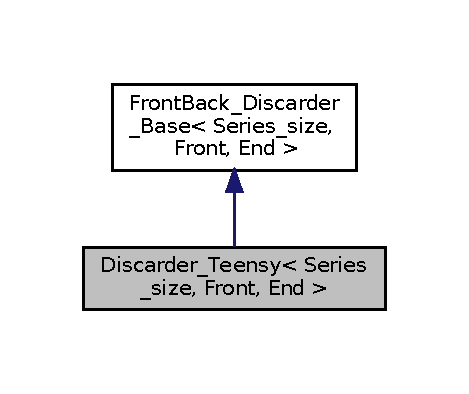
\includegraphics[width=225pt]{classDiscarder__Teensy__inherit__graph}
\end{center}
\end{figure}


Collaboration diagram for Discarder\+\_\+\+Teensy$<$ Series\+\_\+size, Front, End $>$\+:
\nopagebreak
\begin{figure}[H]
\begin{center}
\leavevmode
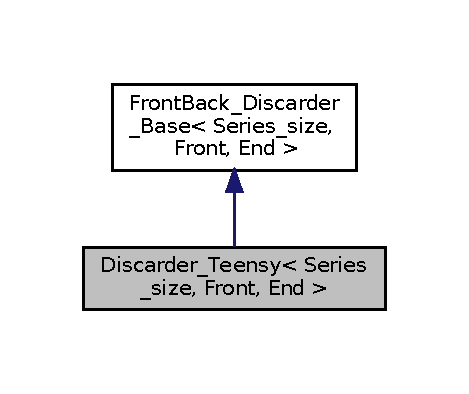
\includegraphics[width=225pt]{classDiscarder__Teensy__coll__graph}
\end{center}
\end{figure}
\subsection*{Private Member Functions}
\begin{DoxyCompactItemize}
\item 
void \hyperlink{classDiscarder__Teensy_a4edb6d02ac299d4c578a4c8522f0dffd}{output} (const \hyperlink{classLin__ACorr__RT__Base}{Lin\+\_\+\+A\+Corr\+\_\+\+R\+T\+\_\+\+Base} \&channel) const override \hyperlink{utilities_8hpp_a103d5b3998e0dd804213c8f30a094f4d}{\+\_\+\+\_\+attribute\+\_\+\+\_\+}((always-\/inline))
\begin{DoxyCompactList}\small\item\em Outputs the channel while discarding the selected channels, by using the implementation specific output method. \end{DoxyCompactList}\end{DoxyCompactItemize}
\subsection*{Additional Inherited Members}


\subsection{Detailed Description}
\subsubsection*{template$<$unsigned int Series\+\_\+size, unsigned int Front, unsigned int End$>$\newline
class Discarder\+\_\+\+Teensy$<$ Series\+\_\+size, Front, End $>$}

Teensy specific Front back discarder implementation. 

\subsection{Member Function Documentation}
\mbox{\Hypertarget{classDiscarder__Teensy_a4edb6d02ac299d4c578a4c8522f0dffd}\label{classDiscarder__Teensy_a4edb6d02ac299d4c578a4c8522f0dffd}} 
\index{Discarder\+\_\+\+Teensy@{Discarder\+\_\+\+Teensy}!output@{output}}
\index{output@{output}!Discarder\+\_\+\+Teensy@{Discarder\+\_\+\+Teensy}}
\subsubsection{\texorpdfstring{output()}{output()}}
{\footnotesize\ttfamily template$<$unsigned int Series\+\_\+size, unsigned int Front, unsigned int End$>$ \\
void \hyperlink{classDiscarder__Teensy}{Discarder\+\_\+\+Teensy}$<$ Series\+\_\+size, Front, End $>$\+::output (\begin{DoxyParamCaption}\item[{const \hyperlink{classLin__ACorr__RT__Base}{Lin\+\_\+\+A\+Corr\+\_\+\+R\+T\+\_\+\+Base} \&}]{channel }\end{DoxyParamCaption}) const\hspace{0.3cm}{\ttfamily [inline]}, {\ttfamily [override]}, {\ttfamily [private]}, {\ttfamily [virtual]}}



Outputs the channel while discarding the selected channels, by using the implementation specific output method. 



Implements \hyperlink{classFrontBack__Discarder__Base_ab8a1d0082f223c31da3c1374c520c4c4}{Front\+Back\+\_\+\+Discarder\+\_\+\+Base$<$ Series\+\_\+size, Front, End $>$}.



The documentation for this class was generated from the following file\+:\begin{DoxyCompactItemize}
\item 
/mnt/m/code/\+Correlator/\+Software/\hyperlink{discarder_8hpp}{discarder.\+hpp}\end{DoxyCompactItemize}

\hypertarget{classFrontBack__Discarder__Base}{}\section{Front\+Back\+\_\+\+Discarder\+\_\+\+Base$<$ Series\+\_\+size, Front, End $>$ Class Template Reference}
\label{classFrontBack__Discarder__Base}\index{Front\+Back\+\_\+\+Discarder\+\_\+\+Base$<$ Series\+\_\+size, Front, End $>$@{Front\+Back\+\_\+\+Discarder\+\_\+\+Base$<$ Series\+\_\+size, Front, End $>$}}


Base class for Front and Back discarder objects.  




{\ttfamily \#include $<$discarder.\+hpp$>$}



Inheritance diagram for Front\+Back\+\_\+\+Discarder\+\_\+\+Base$<$ Series\+\_\+size, Front, End $>$\+:
\nopagebreak
\begin{figure}[H]
\begin{center}
\leavevmode
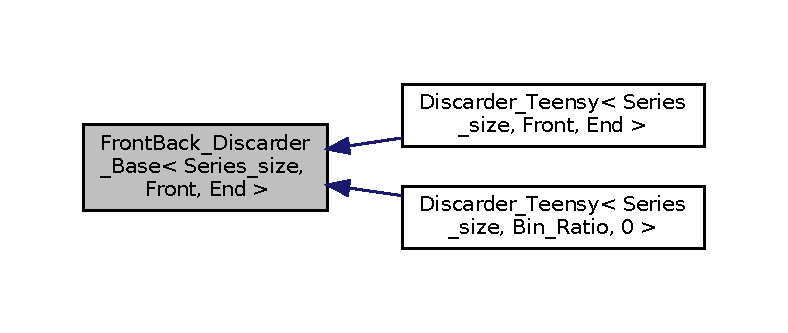
\includegraphics[width=225pt]{classFrontBack__Discarder__Base__inherit__graph}
\end{center}
\end{figure}
\subsection*{Public Member Functions}
\begin{DoxyCompactItemize}
\item 
virtual void const \hyperlink{classFrontBack__Discarder__Base_ab8a1d0082f223c31da3c1374c520c4c4}{output} (const \hyperlink{classLin__ACorr__RT__Base}{Lin\+\_\+\+A\+Corr\+\_\+\+R\+T\+\_\+\+Base} \&channel) const =0
\begin{DoxyCompactList}\small\item\em Outputs the channel while discarding the selected channels, by using the implementation specific output method. \end{DoxyCompactList}\item 
virtual void \hyperlink{classFrontBack__Discarder__Base_a9cc129dd2be2f0894646a3db2aa2bebc}{discards} () const
\begin{DoxyCompactList}\small\item\em Returns the number of elements discarded by the discarder object. \end{DoxyCompactList}\end{DoxyCompactItemize}


\subsection{Detailed Description}
\subsubsection*{template$<$unsigned int Series\+\_\+size, unsigned int Front, unsigned int End$>$\newline
class Front\+Back\+\_\+\+Discarder\+\_\+\+Base$<$ Series\+\_\+size, Front, End $>$}

Base class for Front and Back discarder objects. 

\subsection{Member Function Documentation}
\mbox{\Hypertarget{classFrontBack__Discarder__Base_a9cc129dd2be2f0894646a3db2aa2bebc}\label{classFrontBack__Discarder__Base_a9cc129dd2be2f0894646a3db2aa2bebc}} 
\index{Front\+Back\+\_\+\+Discarder\+\_\+\+Base@{Front\+Back\+\_\+\+Discarder\+\_\+\+Base}!discards@{discards}}
\index{discards@{discards}!Front\+Back\+\_\+\+Discarder\+\_\+\+Base@{Front\+Back\+\_\+\+Discarder\+\_\+\+Base}}
\subsubsection{\texorpdfstring{discards()}{discards()}}
{\footnotesize\ttfamily template$<$unsigned int Series\+\_\+size, unsigned int Front, unsigned int End$>$ \\
virtual void \hyperlink{classFrontBack__Discarder__Base}{Front\+Back\+\_\+\+Discarder\+\_\+\+Base}$<$ Series\+\_\+size, Front, End $>$\+::discards (\begin{DoxyParamCaption}{ }\end{DoxyParamCaption}) const\hspace{0.3cm}{\ttfamily [inline]}, {\ttfamily [virtual]}}



Returns the number of elements discarded by the discarder object. 

\mbox{\Hypertarget{classFrontBack__Discarder__Base_ab8a1d0082f223c31da3c1374c520c4c4}\label{classFrontBack__Discarder__Base_ab8a1d0082f223c31da3c1374c520c4c4}} 
\index{Front\+Back\+\_\+\+Discarder\+\_\+\+Base@{Front\+Back\+\_\+\+Discarder\+\_\+\+Base}!output@{output}}
\index{output@{output}!Front\+Back\+\_\+\+Discarder\+\_\+\+Base@{Front\+Back\+\_\+\+Discarder\+\_\+\+Base}}
\subsubsection{\texorpdfstring{output()}{output()}}
{\footnotesize\ttfamily template$<$unsigned int Series\+\_\+size, unsigned int Front, unsigned int End$>$ \\
virtual void const \hyperlink{classFrontBack__Discarder__Base}{Front\+Back\+\_\+\+Discarder\+\_\+\+Base}$<$ Series\+\_\+size, Front, End $>$\+::output (\begin{DoxyParamCaption}\item[{const \hyperlink{classLin__ACorr__RT__Base}{Lin\+\_\+\+A\+Corr\+\_\+\+R\+T\+\_\+\+Base} \&}]{channel }\end{DoxyParamCaption}) const\hspace{0.3cm}{\ttfamily [inline]}, {\ttfamily [pure virtual]}}



Outputs the channel while discarding the selected channels, by using the implementation specific output method. 



Implemented in \hyperlink{classDiscarder__Teensy_a4edb6d02ac299d4c578a4c8522f0dffd}{Discarder\+\_\+\+Teensy$<$ Series\+\_\+size, Front, End $>$}.



The documentation for this class was generated from the following file\+:\begin{DoxyCompactItemize}
\item 
/mnt/m/code/\+Correlator/\+Software/\hyperlink{discarder_8hpp}{discarder.\+hpp}\end{DoxyCompactItemize}

\hypertarget{classLEDSet}{}\section{L\+E\+D\+Set$<$ S\+E\+T\+\_\+\+S\+I\+ZE $>$ Class Template Reference}
\label{classLEDSet}\index{L\+E\+D\+Set$<$ S\+E\+T\+\_\+\+S\+I\+Z\+E $>$@{L\+E\+D\+Set$<$ S\+E\+T\+\_\+\+S\+I\+Z\+E $>$}}


{\ttfamily \#include $<$ledset.\+hpp$>$}

\subsection*{Public Types}
\begin{DoxyCompactItemize}
\item 
enum \hyperlink{classLEDSet_ae26a13b2d33c51351bc6d0acdf2a94a4}{ledstate\+\_\+t} \{ \hyperlink{classLEDSet_ae26a13b2d33c51351bc6d0acdf2a94a4a786545571f352fd284991e5fcdb79238}{O\+FF} = 0, 
\hyperlink{classLEDSet_ae26a13b2d33c51351bc6d0acdf2a94a4a1e073152d5525648a5bb26cf3eb98ea2}{ON} = 1, 
\hyperlink{classLEDSet_ae26a13b2d33c51351bc6d0acdf2a94a4a2c0806958e37c8d87bd57df8990b30eb}{Analog} = 2
 \}
\end{DoxyCompactItemize}
\subsection*{Public Member Functions}
\begin{DoxyCompactItemize}
\item 
\hyperlink{classLEDSet_a0d3339102ac73fb691f823bcd31a84b9}{L\+E\+D\+Set} (std\+::initializer\+\_\+list$<$ unsigned int $>$ pins)
\begin{DoxyCompactList}\small\item\em Constructor for \hyperlink{classLEDSet}{L\+E\+D\+Set} class. \end{DoxyCompactList}\item 
unsigned int \hyperlink{classLEDSet_a0d153646b1a750421af1f3617d90ad04}{size} () \+\_\+\+\_\+attribute\+\_\+\+\_\+((always\+\_\+inline))
\begin{DoxyCompactList}\small\item\em Returns the size of the led sets. \end{DoxyCompactList}\item 
void \hyperlink{classLEDSet_aae4545d8f8cb6e41a3c2960fb7369e48}{init} ()
\begin{DoxyCompactList}\small\item\em Sets up the pin mode of all L\+E\+Ds. \end{DoxyCompactList}\item 
void \hyperlink{classLEDSet_a520061aaf788486d2aa3aa3dfb3e32d6}{state\+\_\+reload} ()
\begin{DoxyCompactList}\small\item\em Sets the L\+E\+Ds based on the value of the corresponding state variable. This function is useful when the state is altered seperately from the digital\+Write calls. The function also calls pin\+Mode() which muxes the pins to gpio. For State == Analog\+: The state maintains the analog dim state. \end{DoxyCompactList}\item 
void \hyperlink{classLEDSet_a141bb664e7f58ae676455972ca9cd686}{O\+N\+\_\+todigital} ()
\begin{DoxyCompactList}\small\item\em Sets all leds with states (ON == 1) and (Analog == 2) to (ON == 1). \end{DoxyCompactList}\item 
void \hyperlink{classLEDSet_ae2bcd287ff637c2600603e83b0981c77}{toggle\+\_\+all} ()
\begin{DoxyCompactList}\small\item\em Toggles the state of all the L\+E\+Ds. This is a pure digital function and destroys all Analog dim states. \end{DoxyCompactList}\item 
void \hyperlink{classLEDSet_a6062da843aabdf8fbdcedb70fed00dec}{toggle\+\_\+twice} (int pin, double time\+\_\+ms)
\begin{DoxyCompactList}\small\item\em Toggles the state of a particular L\+ED. This is a pure digital function and destroys all Analog dim states. \end{DoxyCompactList}\item 
void \hyperlink{classLEDSet_a61cc024950a5b66dff34c449cc73787f}{toggle\+\_\+all\+\_\+routine} (int delay\+\_\+ms)
\item 
void \hyperlink{classLEDSet_a8a5ef40584236c3793e4274688eac379}{dim} (int pin, unsigned int analog\+\_\+val)
\begin{DoxyCompactList}\small\item\em dims a particular valid led pin. \end{DoxyCompactList}\item 
void \hyperlink{classLEDSet_ad8313aa0c4fc34cd3481db0fade6318c}{dim\+\_\+all} (unsigned int analog\+\_\+val)
\begin{DoxyCompactList}\small\item\em Dims the O\+N-\/\+L\+E\+Ds with the provided analog voltage. Only affects L\+E\+Ds that are ON or on Analog Mode. \end{DoxyCompactList}\item 
void \hyperlink{classLEDSet_a30c6efe7fc286c3d0a7e2ac210dd2c1e}{dim\+\_\+all\+\_\+routine} (unsigned int end\+\_\+analog\+\_\+val, double time\+\_\+s)
\item 
void \hyperlink{classLEDSet_a73dae073882d369a9cc9b9a93f446157}{max\+\_\+bright\+\_\+all} ()
\begin{DoxyCompactList}\small\item\em Sets maximum brightness for all O\+N-\/\+L\+E\+Ds. \end{DoxyCompactList}\item 
void \hyperlink{classLEDSet_a9479e36e91b5b1387cfc27722a4a6007}{min\+\_\+bright\+\_\+all} ()
\item 
void \hyperlink{classLEDSet_aaebfea59ba933621c4f7d7d405119702}{set\+\_\+all} () \+\_\+\+\_\+attribute\+\_\+\+\_\+((always\+\_\+inline))
\begin{DoxyCompactList}\small\item\em Turn on all available L\+E\+Ds. \end{DoxyCompactList}\item 
void \hyperlink{classLEDSet_aabff2609d8df733936dda53d60302b72}{unset\+\_\+all} () \+\_\+\+\_\+attribute\+\_\+\+\_\+((always\+\_\+inline))
\item 
void \hyperlink{classLEDSet_a8f5431c0b3c059c43353cf7e3d02ca62}{set} (int led\+\_\+pin) \+\_\+\+\_\+attribute\+\_\+\+\_\+((always\+\_\+inline))
\begin{DoxyCompactList}\small\item\em Turn-\/\+ON a particular L\+ED Pin. \end{DoxyCompactList}\item 
void \hyperlink{classLEDSet_aacc3566d74c4051350977b578ada3a4d}{unset} (int led\+\_\+pin) \+\_\+\+\_\+attribute\+\_\+\+\_\+((always\+\_\+inline))
\begin{DoxyCompactList}\small\item\em Turn-\/\+O\+FF a particular L\+ED Pin. \end{DoxyCompactList}\item 
void \hyperlink{classLEDSet_a9912385e65dddd78cf0f41cce4fbcba2}{set} (int led\+\_\+pin1, int led\+\_\+pin2) \+\_\+\+\_\+attribute\+\_\+\+\_\+((always\+\_\+inline))
\begin{DoxyCompactList}\small\item\em Turn-\/\+ON two L\+ED Pins simultaneously. The function only works if both the Pins are valid pins. \end{DoxyCompactList}\item 
void \hyperlink{classLEDSet_ac84aa5b9e72689bbfd71f556995dfe03}{unset} (int led\+\_\+pin1, int led\+\_\+pin2) \+\_\+\+\_\+attribute\+\_\+\+\_\+((always\+\_\+inline))
\begin{DoxyCompactList}\small\item\em Turn-\/\+O\+FF two L\+ED Pins simultaneously. \end{DoxyCompactList}\item 
void \hyperlink{classLEDSet_a5dba15c24ec18e11f82368d203ceb9f1}{set} (int led\+\_\+pin1, int led\+\_\+pin2, int led\+\_\+pin3) \+\_\+\+\_\+attribute\+\_\+\+\_\+((always\+\_\+inline))
\begin{DoxyCompactList}\small\item\em Turn-\/\+ON three L\+ED Pins simultaneously. \end{DoxyCompactList}\item 
void \hyperlink{classLEDSet_a1a6a52e4fd96dd8500861df0a9d0066d}{unset} (int led\+\_\+pin1, int led\+\_\+pin2, int led\+\_\+pin3) \+\_\+\+\_\+attribute\+\_\+\+\_\+((always\+\_\+inline))
\begin{DoxyCompactList}\small\item\em Turn-\/\+FF three L\+ED Pins simultaneously. \end{DoxyCompactList}\item 
void \hyperlink{classLEDSet_aa392b74b090de60a25f7577195327afd}{error} (int pin)
\begin{DoxyCompactList}\small\item\em Special function that sets a valid pin and sets the flag {\ttfamily Led\+Set\+::\+Error\+\_\+\+State} to true. This function also clears all L\+ED states prior to the Error State but does not modify states set after the error state. \end{DoxyCompactList}\item 
void \hyperlink{classLEDSet_aafb42531245febe55685c764c29d918f}{assert\+\_\+errors} ()
\begin{DoxyCompactList}\small\item\em Special function that initiates a special routine if the device is in the Error State. It also calls {\ttfamily abort()} , if that feature macro is enabled. \end{DoxyCompactList}\item 
bool \hyperlink{classLEDSet_ab3c7ec4740bab77f762dcd48fba26579}{is\+\_\+valid\+\_\+pin} (int pin)
\begin{DoxyCompactList}\small\item\em Returns whether the given pin is a \char`\"{}valid pin\char`\"{}. A valid pin is a pin that is registered with the \hyperlink{classLEDSet}{L\+E\+D\+Set}. \end{DoxyCompactList}\end{DoxyCompactItemize}
\subsection*{Public Attributes}
\begin{DoxyCompactItemize}
\item 
const int \hyperlink{classLEDSet_a76dfe34c89f6161184583a5ffdcad2e1}{L\+E\+Ds} \mbox{[}S\+E\+T\+\_\+\+S\+I\+ZE\mbox{]} = \{\hyperlink{pins_8hpp_a2b2fb4f846b45d396215a25f949a1bc7}{S\+A\+F\+E\+\_\+\+O\+U\+T\+P\+U\+T\+\_\+\+D\+U\+M\+P\+\_\+\+P\+IN}\}
\begin{DoxyCompactList}\small\item\em L\+ED pins. \end{DoxyCompactList}\item 
unsigned int \hyperlink{classLEDSet_a7185bf98d8866da93847fde7b2145cc4}{State} \mbox{[}S\+E\+T\+\_\+\+S\+I\+ZE\mbox{]}
\begin{DoxyCompactList}\small\item\em O\+N-\/\+O\+F\+F/\+Analog states for all L\+E\+Ds. \end{DoxyCompactList}\item 
bool \hyperlink{classLEDSet_af9c6ea1d0006d7427c82e8e56f9f2de5}{Error\+\_\+\+State} = false
\begin{DoxyCompactList}\small\item\em Whether the L\+ED Panel is in an error state. \end{DoxyCompactList}\end{DoxyCompactItemize}
\subsection*{Private Member Functions}
\begin{DoxyCompactItemize}
\item 
int \hyperlink{classLEDSet_a4ffb3b4a8a5cffdc03f4040ff67a33e9}{fetch\+\_\+index} (int pin) \+\_\+\+\_\+attribute\+\_\+\+\_\+((always\+\_\+inline))
\begin{DoxyCompactList}\small\item\em Retrive data structure index based on the pin number. Returns -\/1 if the pin was not found. \end{DoxyCompactList}\end{DoxyCompactItemize}


\subsection{Detailed Description}
\subsubsection*{template$<$unsigned int S\+E\+T\+\_\+\+S\+I\+ZE$>$\newline
class L\+E\+D\+Set$<$ S\+E\+T\+\_\+\+S\+I\+Z\+E $>$}

an interface for accessing the L\+E\+Ds on the dashboar. The object serves primarily as a bookeeping object, and hence, enables state conservation and switching, and automatically manages dimming, and complex routines. 

\subsection{Member Enumeration Documentation}
\mbox{\Hypertarget{classLEDSet_ae26a13b2d33c51351bc6d0acdf2a94a4}\label{classLEDSet_ae26a13b2d33c51351bc6d0acdf2a94a4}} 
\index{L\+E\+D\+Set@{L\+E\+D\+Set}!ledstate\+\_\+t@{ledstate\+\_\+t}}
\index{ledstate\+\_\+t@{ledstate\+\_\+t}!L\+E\+D\+Set@{L\+E\+D\+Set}}
\subsubsection{\texorpdfstring{ledstate\+\_\+t}{ledstate\_t}}
{\footnotesize\ttfamily template$<$unsigned int S\+E\+T\+\_\+\+S\+I\+ZE$>$ \\
enum \hyperlink{classLEDSet_ae26a13b2d33c51351bc6d0acdf2a94a4}{L\+E\+D\+Set\+::ledstate\+\_\+t}}

\begin{DoxyEnumFields}{Enumerator}
\raisebox{\heightof{T}}[0pt][0pt]{\index{O\+FF@{O\+FF}!L\+E\+D\+Set@{L\+E\+D\+Set}}\index{L\+E\+D\+Set@{L\+E\+D\+Set}!O\+FF@{O\+FF}}}\mbox{\Hypertarget{classLEDSet_ae26a13b2d33c51351bc6d0acdf2a94a4a786545571f352fd284991e5fcdb79238}\label{classLEDSet_ae26a13b2d33c51351bc6d0acdf2a94a4a786545571f352fd284991e5fcdb79238}} 
O\+FF&\\
\hline

\raisebox{\heightof{T}}[0pt][0pt]{\index{ON@{ON}!L\+E\+D\+Set@{L\+E\+D\+Set}}\index{L\+E\+D\+Set@{L\+E\+D\+Set}!ON@{ON}}}\mbox{\Hypertarget{classLEDSet_ae26a13b2d33c51351bc6d0acdf2a94a4a1e073152d5525648a5bb26cf3eb98ea2}\label{classLEDSet_ae26a13b2d33c51351bc6d0acdf2a94a4a1e073152d5525648a5bb26cf3eb98ea2}} 
ON&\\
\hline

\raisebox{\heightof{T}}[0pt][0pt]{\index{Analog@{Analog}!L\+E\+D\+Set@{L\+E\+D\+Set}}\index{L\+E\+D\+Set@{L\+E\+D\+Set}!Analog@{Analog}}}\mbox{\Hypertarget{classLEDSet_ae26a13b2d33c51351bc6d0acdf2a94a4a2c0806958e37c8d87bd57df8990b30eb}\label{classLEDSet_ae26a13b2d33c51351bc6d0acdf2a94a4a2c0806958e37c8d87bd57df8990b30eb}} 
Analog&\\
\hline

\end{DoxyEnumFields}


\subsection{Constructor \& Destructor Documentation}
\mbox{\Hypertarget{classLEDSet_a0d3339102ac73fb691f823bcd31a84b9}\label{classLEDSet_a0d3339102ac73fb691f823bcd31a84b9}} 
\index{L\+E\+D\+Set@{L\+E\+D\+Set}!L\+E\+D\+Set@{L\+E\+D\+Set}}
\index{L\+E\+D\+Set@{L\+E\+D\+Set}!L\+E\+D\+Set@{L\+E\+D\+Set}}
\subsubsection{\texorpdfstring{L\+E\+D\+Set()}{LEDSet()}}
{\footnotesize\ttfamily template$<$unsigned int S\+E\+T\+\_\+\+S\+I\+ZE$>$ \\
\hyperlink{classLEDSet}{L\+E\+D\+Set}$<$ S\+E\+T\+\_\+\+S\+I\+ZE $>$\+::\hyperlink{classLEDSet}{L\+E\+D\+Set} (\begin{DoxyParamCaption}\item[{std\+::initializer\+\_\+list$<$ unsigned int $>$}]{pins }\end{DoxyParamCaption})\hspace{0.3cm}{\ttfamily [inline]}}



Constructor for \hyperlink{classLEDSet}{L\+E\+D\+Set} class. 


\begin{DoxyParams}{Parameters}
{\em pins} & -\/ list of L\+ED pins. \\
\hline
\end{DoxyParams}


\subsection{Member Function Documentation}
\mbox{\Hypertarget{classLEDSet_aafb42531245febe55685c764c29d918f}\label{classLEDSet_aafb42531245febe55685c764c29d918f}} 
\index{L\+E\+D\+Set@{L\+E\+D\+Set}!assert\+\_\+errors@{assert\+\_\+errors}}
\index{assert\+\_\+errors@{assert\+\_\+errors}!L\+E\+D\+Set@{L\+E\+D\+Set}}
\subsubsection{\texorpdfstring{assert\+\_\+errors()}{assert\_errors()}}
{\footnotesize\ttfamily template$<$unsigned int S\+E\+T\+\_\+\+S\+I\+ZE$>$ \\
void \hyperlink{classLEDSet}{L\+E\+D\+Set}$<$ S\+E\+T\+\_\+\+S\+I\+ZE $>$\+::assert\+\_\+errors (\begin{DoxyParamCaption}{ }\end{DoxyParamCaption})\hspace{0.3cm}{\ttfamily [inline]}}



Special function that initiates a special routine if the device is in the Error State. It also calls {\ttfamily abort()} , if that feature macro is enabled. 

\mbox{\Hypertarget{classLEDSet_a8a5ef40584236c3793e4274688eac379}\label{classLEDSet_a8a5ef40584236c3793e4274688eac379}} 
\index{L\+E\+D\+Set@{L\+E\+D\+Set}!dim@{dim}}
\index{dim@{dim}!L\+E\+D\+Set@{L\+E\+D\+Set}}
\subsubsection{\texorpdfstring{dim()}{dim()}}
{\footnotesize\ttfamily template$<$unsigned int S\+E\+T\+\_\+\+S\+I\+ZE$>$ \\
void \hyperlink{classLEDSet}{L\+E\+D\+Set}$<$ S\+E\+T\+\_\+\+S\+I\+ZE $>$\+::dim (\begin{DoxyParamCaption}\item[{int}]{pin,  }\item[{unsigned int}]{analog\+\_\+val }\end{DoxyParamCaption})\hspace{0.3cm}{\ttfamily [inline]}}



dims a particular valid led pin. 

\mbox{\Hypertarget{classLEDSet_ad8313aa0c4fc34cd3481db0fade6318c}\label{classLEDSet_ad8313aa0c4fc34cd3481db0fade6318c}} 
\index{L\+E\+D\+Set@{L\+E\+D\+Set}!dim\+\_\+all@{dim\+\_\+all}}
\index{dim\+\_\+all@{dim\+\_\+all}!L\+E\+D\+Set@{L\+E\+D\+Set}}
\subsubsection{\texorpdfstring{dim\+\_\+all()}{dim\_all()}}
{\footnotesize\ttfamily template$<$unsigned int S\+E\+T\+\_\+\+S\+I\+ZE$>$ \\
void \hyperlink{classLEDSet}{L\+E\+D\+Set}$<$ S\+E\+T\+\_\+\+S\+I\+ZE $>$\+::dim\+\_\+all (\begin{DoxyParamCaption}\item[{unsigned int}]{analog\+\_\+val }\end{DoxyParamCaption})\hspace{0.3cm}{\ttfamily [inline]}}



Dims the O\+N-\/\+L\+E\+Ds with the provided analog voltage. Only affects L\+E\+Ds that are ON or on Analog Mode. 

\mbox{\Hypertarget{classLEDSet_a30c6efe7fc286c3d0a7e2ac210dd2c1e}\label{classLEDSet_a30c6efe7fc286c3d0a7e2ac210dd2c1e}} 
\index{L\+E\+D\+Set@{L\+E\+D\+Set}!dim\+\_\+all\+\_\+routine@{dim\+\_\+all\+\_\+routine}}
\index{dim\+\_\+all\+\_\+routine@{dim\+\_\+all\+\_\+routine}!L\+E\+D\+Set@{L\+E\+D\+Set}}
\subsubsection{\texorpdfstring{dim\+\_\+all\+\_\+routine()}{dim\_all\_routine()}}
{\footnotesize\ttfamily template$<$unsigned int S\+E\+T\+\_\+\+S\+I\+ZE$>$ \\
void \hyperlink{classLEDSet}{L\+E\+D\+Set}$<$ S\+E\+T\+\_\+\+S\+I\+ZE $>$\+::dim\+\_\+all\+\_\+routine (\begin{DoxyParamCaption}\item[{unsigned int}]{end\+\_\+analog\+\_\+val,  }\item[{double}]{time\+\_\+s }\end{DoxyParamCaption})\hspace{0.3cm}{\ttfamily [inline]}}

\mbox{\Hypertarget{classLEDSet_aa392b74b090de60a25f7577195327afd}\label{classLEDSet_aa392b74b090de60a25f7577195327afd}} 
\index{L\+E\+D\+Set@{L\+E\+D\+Set}!error@{error}}
\index{error@{error}!L\+E\+D\+Set@{L\+E\+D\+Set}}
\subsubsection{\texorpdfstring{error()}{error()}}
{\footnotesize\ttfamily template$<$unsigned int S\+E\+T\+\_\+\+S\+I\+ZE$>$ \\
void \hyperlink{classLEDSet}{L\+E\+D\+Set}$<$ S\+E\+T\+\_\+\+S\+I\+ZE $>$\+::error (\begin{DoxyParamCaption}\item[{int}]{pin }\end{DoxyParamCaption})\hspace{0.3cm}{\ttfamily [inline]}}



Special function that sets a valid pin and sets the flag {\ttfamily Led\+Set\+::\+Error\+\_\+\+State} to true. This function also clears all L\+ED states prior to the Error State but does not modify states set after the error state. 

\mbox{\Hypertarget{classLEDSet_a4ffb3b4a8a5cffdc03f4040ff67a33e9}\label{classLEDSet_a4ffb3b4a8a5cffdc03f4040ff67a33e9}} 
\index{L\+E\+D\+Set@{L\+E\+D\+Set}!fetch\+\_\+index@{fetch\+\_\+index}}
\index{fetch\+\_\+index@{fetch\+\_\+index}!L\+E\+D\+Set@{L\+E\+D\+Set}}
\subsubsection{\texorpdfstring{fetch\+\_\+index()}{fetch\_index()}}
{\footnotesize\ttfamily template$<$unsigned int S\+E\+T\+\_\+\+S\+I\+ZE$>$ \\
int \hyperlink{classLEDSet}{L\+E\+D\+Set}$<$ S\+E\+T\+\_\+\+S\+I\+ZE $>$\+::fetch\+\_\+index (\begin{DoxyParamCaption}\item[{int}]{pin }\end{DoxyParamCaption})\hspace{0.3cm}{\ttfamily [inline]}, {\ttfamily [private]}}



Retrive data structure index based on the pin number. Returns -\/1 if the pin was not found. 

\begin{DoxyReturn}{Returns}
Local array index of pin in the L\+E\+Ds array (bookeeping object). -\/1 if the search fails. 
\end{DoxyReturn}
\mbox{\Hypertarget{classLEDSet_aae4545d8f8cb6e41a3c2960fb7369e48}\label{classLEDSet_aae4545d8f8cb6e41a3c2960fb7369e48}} 
\index{L\+E\+D\+Set@{L\+E\+D\+Set}!init@{init}}
\index{init@{init}!L\+E\+D\+Set@{L\+E\+D\+Set}}
\subsubsection{\texorpdfstring{init()}{init()}}
{\footnotesize\ttfamily template$<$unsigned int S\+E\+T\+\_\+\+S\+I\+ZE$>$ \\
void \hyperlink{classLEDSet}{L\+E\+D\+Set}$<$ S\+E\+T\+\_\+\+S\+I\+ZE $>$\+::init (\begin{DoxyParamCaption}{ }\end{DoxyParamCaption})\hspace{0.3cm}{\ttfamily [inline]}}



Sets up the pin mode of all L\+E\+Ds. 

\mbox{\Hypertarget{classLEDSet_ab3c7ec4740bab77f762dcd48fba26579}\label{classLEDSet_ab3c7ec4740bab77f762dcd48fba26579}} 
\index{L\+E\+D\+Set@{L\+E\+D\+Set}!is\+\_\+valid\+\_\+pin@{is\+\_\+valid\+\_\+pin}}
\index{is\+\_\+valid\+\_\+pin@{is\+\_\+valid\+\_\+pin}!L\+E\+D\+Set@{L\+E\+D\+Set}}
\subsubsection{\texorpdfstring{is\+\_\+valid\+\_\+pin()}{is\_valid\_pin()}}
{\footnotesize\ttfamily template$<$unsigned int S\+E\+T\+\_\+\+S\+I\+ZE$>$ \\
bool \hyperlink{classLEDSet}{L\+E\+D\+Set}$<$ S\+E\+T\+\_\+\+S\+I\+ZE $>$\+::is\+\_\+valid\+\_\+pin (\begin{DoxyParamCaption}\item[{int}]{pin }\end{DoxyParamCaption})\hspace{0.3cm}{\ttfamily [inline]}}



Returns whether the given pin is a \char`\"{}valid pin\char`\"{}. A valid pin is a pin that is registered with the \hyperlink{classLEDSet}{L\+E\+D\+Set}. 

\mbox{\Hypertarget{classLEDSet_a73dae073882d369a9cc9b9a93f446157}\label{classLEDSet_a73dae073882d369a9cc9b9a93f446157}} 
\index{L\+E\+D\+Set@{L\+E\+D\+Set}!max\+\_\+bright\+\_\+all@{max\+\_\+bright\+\_\+all}}
\index{max\+\_\+bright\+\_\+all@{max\+\_\+bright\+\_\+all}!L\+E\+D\+Set@{L\+E\+D\+Set}}
\subsubsection{\texorpdfstring{max\+\_\+bright\+\_\+all()}{max\_bright\_all()}}
{\footnotesize\ttfamily template$<$unsigned int S\+E\+T\+\_\+\+S\+I\+ZE$>$ \\
void \hyperlink{classLEDSet}{L\+E\+D\+Set}$<$ S\+E\+T\+\_\+\+S\+I\+ZE $>$\+::max\+\_\+bright\+\_\+all (\begin{DoxyParamCaption}{ }\end{DoxyParamCaption})\hspace{0.3cm}{\ttfamily [inline]}}



Sets maximum brightness for all O\+N-\/\+L\+E\+Ds. 

\mbox{\Hypertarget{classLEDSet_a9479e36e91b5b1387cfc27722a4a6007}\label{classLEDSet_a9479e36e91b5b1387cfc27722a4a6007}} 
\index{L\+E\+D\+Set@{L\+E\+D\+Set}!min\+\_\+bright\+\_\+all@{min\+\_\+bright\+\_\+all}}
\index{min\+\_\+bright\+\_\+all@{min\+\_\+bright\+\_\+all}!L\+E\+D\+Set@{L\+E\+D\+Set}}
\subsubsection{\texorpdfstring{min\+\_\+bright\+\_\+all()}{min\_bright\_all()}}
{\footnotesize\ttfamily template$<$unsigned int S\+E\+T\+\_\+\+S\+I\+ZE$>$ \\
void \hyperlink{classLEDSet}{L\+E\+D\+Set}$<$ S\+E\+T\+\_\+\+S\+I\+ZE $>$\+::min\+\_\+bright\+\_\+all (\begin{DoxyParamCaption}{ }\end{DoxyParamCaption})\hspace{0.3cm}{\ttfamily [inline]}}

Sets the minimum brighness for all O\+N-\/\+L\+E\+Ds. \mbox{\Hypertarget{classLEDSet_a141bb664e7f58ae676455972ca9cd686}\label{classLEDSet_a141bb664e7f58ae676455972ca9cd686}} 
\index{L\+E\+D\+Set@{L\+E\+D\+Set}!O\+N\+\_\+todigital@{O\+N\+\_\+todigital}}
\index{O\+N\+\_\+todigital@{O\+N\+\_\+todigital}!L\+E\+D\+Set@{L\+E\+D\+Set}}
\subsubsection{\texorpdfstring{O\+N\+\_\+todigital()}{ON\_todigital()}}
{\footnotesize\ttfamily template$<$unsigned int S\+E\+T\+\_\+\+S\+I\+ZE$>$ \\
void \hyperlink{classLEDSet}{L\+E\+D\+Set}$<$ S\+E\+T\+\_\+\+S\+I\+ZE $>$\+::O\+N\+\_\+todigital (\begin{DoxyParamCaption}{ }\end{DoxyParamCaption})\hspace{0.3cm}{\ttfamily [inline]}}



Sets all leds with states (ON == 1) and (Analog == 2) to (ON == 1). 

\mbox{\Hypertarget{classLEDSet_a8f5431c0b3c059c43353cf7e3d02ca62}\label{classLEDSet_a8f5431c0b3c059c43353cf7e3d02ca62}} 
\index{L\+E\+D\+Set@{L\+E\+D\+Set}!set@{set}}
\index{set@{set}!L\+E\+D\+Set@{L\+E\+D\+Set}}
\subsubsection{\texorpdfstring{set()}{set()}\hspace{0.1cm}{\footnotesize\ttfamily [1/3]}}
{\footnotesize\ttfamily template$<$unsigned int S\+E\+T\+\_\+\+S\+I\+ZE$>$ \\
void \hyperlink{classLEDSet}{L\+E\+D\+Set}$<$ S\+E\+T\+\_\+\+S\+I\+ZE $>$\+::set (\begin{DoxyParamCaption}\item[{int}]{led\+\_\+pin }\end{DoxyParamCaption})\hspace{0.3cm}{\ttfamily [inline]}}



Turn-\/\+ON a particular L\+ED Pin. 

\mbox{\Hypertarget{classLEDSet_a9912385e65dddd78cf0f41cce4fbcba2}\label{classLEDSet_a9912385e65dddd78cf0f41cce4fbcba2}} 
\index{L\+E\+D\+Set@{L\+E\+D\+Set}!set@{set}}
\index{set@{set}!L\+E\+D\+Set@{L\+E\+D\+Set}}
\subsubsection{\texorpdfstring{set()}{set()}\hspace{0.1cm}{\footnotesize\ttfamily [2/3]}}
{\footnotesize\ttfamily template$<$unsigned int S\+E\+T\+\_\+\+S\+I\+ZE$>$ \\
void \hyperlink{classLEDSet}{L\+E\+D\+Set}$<$ S\+E\+T\+\_\+\+S\+I\+ZE $>$\+::set (\begin{DoxyParamCaption}\item[{int}]{led\+\_\+pin1,  }\item[{int}]{led\+\_\+pin2 }\end{DoxyParamCaption})\hspace{0.3cm}{\ttfamily [inline]}}



Turn-\/\+ON two L\+ED Pins simultaneously. The function only works if both the Pins are valid pins. 

\mbox{\Hypertarget{classLEDSet_a5dba15c24ec18e11f82368d203ceb9f1}\label{classLEDSet_a5dba15c24ec18e11f82368d203ceb9f1}} 
\index{L\+E\+D\+Set@{L\+E\+D\+Set}!set@{set}}
\index{set@{set}!L\+E\+D\+Set@{L\+E\+D\+Set}}
\subsubsection{\texorpdfstring{set()}{set()}\hspace{0.1cm}{\footnotesize\ttfamily [3/3]}}
{\footnotesize\ttfamily template$<$unsigned int S\+E\+T\+\_\+\+S\+I\+ZE$>$ \\
void \hyperlink{classLEDSet}{L\+E\+D\+Set}$<$ S\+E\+T\+\_\+\+S\+I\+ZE $>$\+::set (\begin{DoxyParamCaption}\item[{int}]{led\+\_\+pin1,  }\item[{int}]{led\+\_\+pin2,  }\item[{int}]{led\+\_\+pin3 }\end{DoxyParamCaption})\hspace{0.3cm}{\ttfamily [inline]}}



Turn-\/\+ON three L\+ED Pins simultaneously. 

\mbox{\Hypertarget{classLEDSet_aaebfea59ba933621c4f7d7d405119702}\label{classLEDSet_aaebfea59ba933621c4f7d7d405119702}} 
\index{L\+E\+D\+Set@{L\+E\+D\+Set}!set\+\_\+all@{set\+\_\+all}}
\index{set\+\_\+all@{set\+\_\+all}!L\+E\+D\+Set@{L\+E\+D\+Set}}
\subsubsection{\texorpdfstring{set\+\_\+all()}{set\_all()}}
{\footnotesize\ttfamily template$<$unsigned int S\+E\+T\+\_\+\+S\+I\+ZE$>$ \\
void \hyperlink{classLEDSet}{L\+E\+D\+Set}$<$ S\+E\+T\+\_\+\+S\+I\+ZE $>$\+::set\+\_\+all (\begin{DoxyParamCaption}{ }\end{DoxyParamCaption})\hspace{0.3cm}{\ttfamily [inline]}}



Turn on all available L\+E\+Ds. 

\mbox{\Hypertarget{classLEDSet_a0d153646b1a750421af1f3617d90ad04}\label{classLEDSet_a0d153646b1a750421af1f3617d90ad04}} 
\index{L\+E\+D\+Set@{L\+E\+D\+Set}!size@{size}}
\index{size@{size}!L\+E\+D\+Set@{L\+E\+D\+Set}}
\subsubsection{\texorpdfstring{size()}{size()}}
{\footnotesize\ttfamily template$<$unsigned int S\+E\+T\+\_\+\+S\+I\+ZE$>$ \\
unsigned int \hyperlink{classLEDSet}{L\+E\+D\+Set}$<$ S\+E\+T\+\_\+\+S\+I\+ZE $>$\+::size (\begin{DoxyParamCaption}{ }\end{DoxyParamCaption})\hspace{0.3cm}{\ttfamily [inline]}}



Returns the size of the led sets. 

\mbox{\Hypertarget{classLEDSet_a520061aaf788486d2aa3aa3dfb3e32d6}\label{classLEDSet_a520061aaf788486d2aa3aa3dfb3e32d6}} 
\index{L\+E\+D\+Set@{L\+E\+D\+Set}!state\+\_\+reload@{state\+\_\+reload}}
\index{state\+\_\+reload@{state\+\_\+reload}!L\+E\+D\+Set@{L\+E\+D\+Set}}
\subsubsection{\texorpdfstring{state\+\_\+reload()}{state\_reload()}}
{\footnotesize\ttfamily template$<$unsigned int S\+E\+T\+\_\+\+S\+I\+ZE$>$ \\
void \hyperlink{classLEDSet}{L\+E\+D\+Set}$<$ S\+E\+T\+\_\+\+S\+I\+ZE $>$\+::state\+\_\+reload (\begin{DoxyParamCaption}{ }\end{DoxyParamCaption})\hspace{0.3cm}{\ttfamily [inline]}}



Sets the L\+E\+Ds based on the value of the corresponding state variable. This function is useful when the state is altered seperately from the digital\+Write calls. The function also calls pin\+Mode() which muxes the pins to gpio. For State == Analog\+: The state maintains the analog dim state. 

\mbox{\Hypertarget{classLEDSet_ae2bcd287ff637c2600603e83b0981c77}\label{classLEDSet_ae2bcd287ff637c2600603e83b0981c77}} 
\index{L\+E\+D\+Set@{L\+E\+D\+Set}!toggle\+\_\+all@{toggle\+\_\+all}}
\index{toggle\+\_\+all@{toggle\+\_\+all}!L\+E\+D\+Set@{L\+E\+D\+Set}}
\subsubsection{\texorpdfstring{toggle\+\_\+all()}{toggle\_all()}}
{\footnotesize\ttfamily template$<$unsigned int S\+E\+T\+\_\+\+S\+I\+ZE$>$ \\
void \hyperlink{classLEDSet}{L\+E\+D\+Set}$<$ S\+E\+T\+\_\+\+S\+I\+ZE $>$\+::toggle\+\_\+all (\begin{DoxyParamCaption}{ }\end{DoxyParamCaption})\hspace{0.3cm}{\ttfamily [inline]}}



Toggles the state of all the L\+E\+Ds. This is a pure digital function and destroys all Analog dim states. 

\mbox{\Hypertarget{classLEDSet_a61cc024950a5b66dff34c449cc73787f}\label{classLEDSet_a61cc024950a5b66dff34c449cc73787f}} 
\index{L\+E\+D\+Set@{L\+E\+D\+Set}!toggle\+\_\+all\+\_\+routine@{toggle\+\_\+all\+\_\+routine}}
\index{toggle\+\_\+all\+\_\+routine@{toggle\+\_\+all\+\_\+routine}!L\+E\+D\+Set@{L\+E\+D\+Set}}
\subsubsection{\texorpdfstring{toggle\+\_\+all\+\_\+routine()}{toggle\_all\_routine()}}
{\footnotesize\ttfamily template$<$unsigned int S\+E\+T\+\_\+\+S\+I\+ZE$>$ \\
void \hyperlink{classLEDSet}{L\+E\+D\+Set}$<$ S\+E\+T\+\_\+\+S\+I\+ZE $>$\+::toggle\+\_\+all\+\_\+routine (\begin{DoxyParamCaption}\item[{int}]{delay\+\_\+ms }\end{DoxyParamCaption})\hspace{0.3cm}{\ttfamily [inline]}}

\mbox{\Hypertarget{classLEDSet_a6062da843aabdf8fbdcedb70fed00dec}\label{classLEDSet_a6062da843aabdf8fbdcedb70fed00dec}} 
\index{L\+E\+D\+Set@{L\+E\+D\+Set}!toggle\+\_\+twice@{toggle\+\_\+twice}}
\index{toggle\+\_\+twice@{toggle\+\_\+twice}!L\+E\+D\+Set@{L\+E\+D\+Set}}
\subsubsection{\texorpdfstring{toggle\+\_\+twice()}{toggle\_twice()}}
{\footnotesize\ttfamily template$<$unsigned int S\+E\+T\+\_\+\+S\+I\+ZE$>$ \\
void \hyperlink{classLEDSet}{L\+E\+D\+Set}$<$ S\+E\+T\+\_\+\+S\+I\+ZE $>$\+::toggle\+\_\+twice (\begin{DoxyParamCaption}\item[{int}]{pin,  }\item[{double}]{time\+\_\+ms }\end{DoxyParamCaption})\hspace{0.3cm}{\ttfamily [inline]}}



Toggles the state of a particular L\+ED. This is a pure digital function and destroys all Analog dim states. 

\mbox{\Hypertarget{classLEDSet_aacc3566d74c4051350977b578ada3a4d}\label{classLEDSet_aacc3566d74c4051350977b578ada3a4d}} 
\index{L\+E\+D\+Set@{L\+E\+D\+Set}!unset@{unset}}
\index{unset@{unset}!L\+E\+D\+Set@{L\+E\+D\+Set}}
\subsubsection{\texorpdfstring{unset()}{unset()}\hspace{0.1cm}{\footnotesize\ttfamily [1/3]}}
{\footnotesize\ttfamily template$<$unsigned int S\+E\+T\+\_\+\+S\+I\+ZE$>$ \\
void \hyperlink{classLEDSet}{L\+E\+D\+Set}$<$ S\+E\+T\+\_\+\+S\+I\+ZE $>$\+::unset (\begin{DoxyParamCaption}\item[{int}]{led\+\_\+pin }\end{DoxyParamCaption})\hspace{0.3cm}{\ttfamily [inline]}}



Turn-\/\+O\+FF a particular L\+ED Pin. 

\mbox{\Hypertarget{classLEDSet_ac84aa5b9e72689bbfd71f556995dfe03}\label{classLEDSet_ac84aa5b9e72689bbfd71f556995dfe03}} 
\index{L\+E\+D\+Set@{L\+E\+D\+Set}!unset@{unset}}
\index{unset@{unset}!L\+E\+D\+Set@{L\+E\+D\+Set}}
\subsubsection{\texorpdfstring{unset()}{unset()}\hspace{0.1cm}{\footnotesize\ttfamily [2/3]}}
{\footnotesize\ttfamily template$<$unsigned int S\+E\+T\+\_\+\+S\+I\+ZE$>$ \\
void \hyperlink{classLEDSet}{L\+E\+D\+Set}$<$ S\+E\+T\+\_\+\+S\+I\+ZE $>$\+::unset (\begin{DoxyParamCaption}\item[{int}]{led\+\_\+pin1,  }\item[{int}]{led\+\_\+pin2 }\end{DoxyParamCaption})\hspace{0.3cm}{\ttfamily [inline]}}



Turn-\/\+O\+FF two L\+ED Pins simultaneously. 

\mbox{\Hypertarget{classLEDSet_a1a6a52e4fd96dd8500861df0a9d0066d}\label{classLEDSet_a1a6a52e4fd96dd8500861df0a9d0066d}} 
\index{L\+E\+D\+Set@{L\+E\+D\+Set}!unset@{unset}}
\index{unset@{unset}!L\+E\+D\+Set@{L\+E\+D\+Set}}
\subsubsection{\texorpdfstring{unset()}{unset()}\hspace{0.1cm}{\footnotesize\ttfamily [3/3]}}
{\footnotesize\ttfamily template$<$unsigned int S\+E\+T\+\_\+\+S\+I\+ZE$>$ \\
void \hyperlink{classLEDSet}{L\+E\+D\+Set}$<$ S\+E\+T\+\_\+\+S\+I\+ZE $>$\+::unset (\begin{DoxyParamCaption}\item[{int}]{led\+\_\+pin1,  }\item[{int}]{led\+\_\+pin2,  }\item[{int}]{led\+\_\+pin3 }\end{DoxyParamCaption})\hspace{0.3cm}{\ttfamily [inline]}}



Turn-\/\+FF three L\+ED Pins simultaneously. 

\mbox{\Hypertarget{classLEDSet_aabff2609d8df733936dda53d60302b72}\label{classLEDSet_aabff2609d8df733936dda53d60302b72}} 
\index{L\+E\+D\+Set@{L\+E\+D\+Set}!unset\+\_\+all@{unset\+\_\+all}}
\index{unset\+\_\+all@{unset\+\_\+all}!L\+E\+D\+Set@{L\+E\+D\+Set}}
\subsubsection{\texorpdfstring{unset\+\_\+all()}{unset\_all()}}
{\footnotesize\ttfamily template$<$unsigned int S\+E\+T\+\_\+\+S\+I\+ZE$>$ \\
void \hyperlink{classLEDSet}{L\+E\+D\+Set}$<$ S\+E\+T\+\_\+\+S\+I\+ZE $>$\+::unset\+\_\+all (\begin{DoxyParamCaption}{ }\end{DoxyParamCaption})\hspace{0.3cm}{\ttfamily [inline]}}

Turn off all available L\+E\+Ds. 

\subsection{Member Data Documentation}
\mbox{\Hypertarget{classLEDSet_af9c6ea1d0006d7427c82e8e56f9f2de5}\label{classLEDSet_af9c6ea1d0006d7427c82e8e56f9f2de5}} 
\index{L\+E\+D\+Set@{L\+E\+D\+Set}!Error\+\_\+\+State@{Error\+\_\+\+State}}
\index{Error\+\_\+\+State@{Error\+\_\+\+State}!L\+E\+D\+Set@{L\+E\+D\+Set}}
\subsubsection{\texorpdfstring{Error\+\_\+\+State}{Error\_State}}
{\footnotesize\ttfamily template$<$unsigned int S\+E\+T\+\_\+\+S\+I\+ZE$>$ \\
bool \hyperlink{classLEDSet}{L\+E\+D\+Set}$<$ S\+E\+T\+\_\+\+S\+I\+ZE $>$\+::Error\+\_\+\+State = false}



Whether the L\+ED Panel is in an error state. 

\mbox{\Hypertarget{classLEDSet_a76dfe34c89f6161184583a5ffdcad2e1}\label{classLEDSet_a76dfe34c89f6161184583a5ffdcad2e1}} 
\index{L\+E\+D\+Set@{L\+E\+D\+Set}!L\+E\+Ds@{L\+E\+Ds}}
\index{L\+E\+Ds@{L\+E\+Ds}!L\+E\+D\+Set@{L\+E\+D\+Set}}
\subsubsection{\texorpdfstring{L\+E\+Ds}{LEDs}}
{\footnotesize\ttfamily template$<$unsigned int S\+E\+T\+\_\+\+S\+I\+ZE$>$ \\
const int \hyperlink{classLEDSet}{L\+E\+D\+Set}$<$ S\+E\+T\+\_\+\+S\+I\+ZE $>$\+::L\+E\+Ds\mbox{[}S\+E\+T\+\_\+\+S\+I\+ZE\mbox{]} = \{\hyperlink{pins_8hpp_a2b2fb4f846b45d396215a25f949a1bc7}{S\+A\+F\+E\+\_\+\+O\+U\+T\+P\+U\+T\+\_\+\+D\+U\+M\+P\+\_\+\+P\+IN}\}}



L\+ED pins. 

\mbox{\Hypertarget{classLEDSet_a7185bf98d8866da93847fde7b2145cc4}\label{classLEDSet_a7185bf98d8866da93847fde7b2145cc4}} 
\index{L\+E\+D\+Set@{L\+E\+D\+Set}!State@{State}}
\index{State@{State}!L\+E\+D\+Set@{L\+E\+D\+Set}}
\subsubsection{\texorpdfstring{State}{State}}
{\footnotesize\ttfamily template$<$unsigned int S\+E\+T\+\_\+\+S\+I\+ZE$>$ \\
unsigned int \hyperlink{classLEDSet}{L\+E\+D\+Set}$<$ S\+E\+T\+\_\+\+S\+I\+ZE $>$\+::State\mbox{[}S\+E\+T\+\_\+\+S\+I\+ZE\mbox{]}}



O\+N-\/\+O\+F\+F/\+Analog states for all L\+E\+Ds. 



The documentation for this class was generated from the following file\+:\begin{DoxyCompactItemize}
\item 
code/hardware/\hyperlink{ledset_8hpp}{ledset.\+hpp}\end{DoxyCompactItemize}

\hypertarget{classLin__ACorr__RT__Base}{}\section{Lin\+\_\+\+A\+Corr\+\_\+\+R\+T\+\_\+\+Base Class Reference}
\label{classLin__ACorr__RT__Base}\index{Lin\+\_\+\+A\+Corr\+\_\+\+R\+T\+\_\+\+Base@{Lin\+\_\+\+A\+Corr\+\_\+\+R\+T\+\_\+\+Base}}


This class is a blank interface for all objects that are — {\bfseries \{Linear} Real-\/\+Time Software Auto-\/\+Correlators\}.  




{\ttfamily \#include $<$Lin\+\_\+\+A\+Corr\+\_\+\+R\+T\+\_\+\+Base.\+hpp$>$}



Inheritance diagram for Lin\+\_\+\+A\+Corr\+\_\+\+R\+T\+\_\+\+Base\+:\nopagebreak
\begin{figure}[H]
\begin{center}
\leavevmode
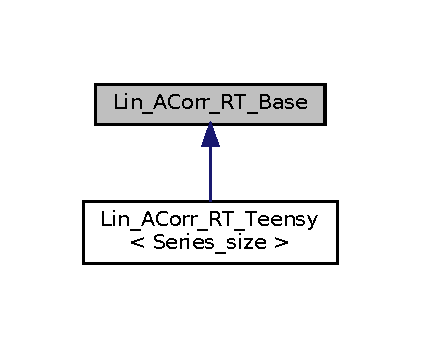
\includegraphics[width=202pt]{classLin__ACorr__RT__Base__inherit__graph}
\end{center}
\end{figure}
\subsection*{Public Member Functions}
\begin{DoxyCompactItemize}
\item 
virtual void \hyperlink{classLin__ACorr__RT__Base_a398167525faf2a65f29722e943a0c57e}{push\+\_\+datum} (\hyperlink{types_8hpp_a22f279793847eba127de149437848c48}{counter\+\_\+t} datum)=0
\begin{DoxyCompactList}\small\item\em Accepts a single {\ttfamily datum} from the counter — which is the lowest order of data aggregate, appends to Series\+\_\+array and updates relevant channels. \end{DoxyCompactList}\item 
virtual void \hyperlink{classLin__ACorr__RT__Base_a91c95a49619995f40aeae80916afed3e}{push\+\_\+data} (const \hyperlink{types_8hpp_a22f279793847eba127de149437848c48}{counter\+\_\+t} $\ast$container, const index\+\_\+t size)=0
\begin{DoxyCompactList}\small\item\em Repeatedy calls {\ttfamily Lin\+\_\+\+A\+Corr\+\_\+\+R\+T\+\_\+\+Base\+::push\+\_\+datam()} on all the elements of the countainer. \end{DoxyCompactList}\item 
virtual double \hyperlink{classLin__ACorr__RT__Base_a06c0bbe593f87a9034aa34e95d9d46db}{norm} (index\+\_\+t lag)=0
\begin{DoxyCompactList}\small\item\em Takes in the lag value and returns the normalization (divider) for the passed lag value. \end{DoxyCompactList}\item 
virtual void \hyperlink{group__Lin__ACorr__Base__Out_ga4fe3bd7a6a98388d46827d22dc4596c9}{ch\+\_\+out} () const =0
\begin{DoxyCompactList}\small\item\em Outputs all the channels using specific implementation based methods. \end{DoxyCompactList}\item 
virtual void \hyperlink{group__Lin__ACorr__Base__Out_ga3e58cb03c3a93107758d506c53cf2461}{ch\+\_\+out\+\_\+norm} () const =0
\begin{DoxyCompactList}\small\item\em Outputs all the channels with {\bfseries } $<$normalisation$>$ using specific implementation based methods. \end{DoxyCompactList}\item 
virtual \hyperlink{types_8hpp_a22f279793847eba127de149437848c48}{counter\+\_\+t} $\ast$ \hyperlink{group__Lin__ACorr__Base__Out_gafb6585805776a54d5e4f120cfd1fea9e}{get\+\_\+ch\+\_\+array} () const =0
\end{DoxyCompactItemize}


\subsection{Detailed Description}
This class is a blank interface for all objects that are — {\bfseries \{Linear} Real-\/\+Time Software Auto-\/\+Correlators\}. 

\subsection{Member Function Documentation}
\mbox{\Hypertarget{classLin__ACorr__RT__Base_a06c0bbe593f87a9034aa34e95d9d46db}\label{classLin__ACorr__RT__Base_a06c0bbe593f87a9034aa34e95d9d46db}} 
\index{Lin\+\_\+\+A\+Corr\+\_\+\+R\+T\+\_\+\+Base@{Lin\+\_\+\+A\+Corr\+\_\+\+R\+T\+\_\+\+Base}!norm@{norm}}
\index{norm@{norm}!Lin\+\_\+\+A\+Corr\+\_\+\+R\+T\+\_\+\+Base@{Lin\+\_\+\+A\+Corr\+\_\+\+R\+T\+\_\+\+Base}}
\subsubsection{\texorpdfstring{norm()}{norm()}}
{\footnotesize\ttfamily virtual double Lin\+\_\+\+A\+Corr\+\_\+\+R\+T\+\_\+\+Base\+::norm (\begin{DoxyParamCaption}\item[{index\+\_\+t}]{lag }\end{DoxyParamCaption})\hspace{0.3cm}{\ttfamily [inline]}, {\ttfamily [pure virtual]}}



Takes in the lag value and returns the normalization (divider) for the passed lag value. 

\mbox{\Hypertarget{classLin__ACorr__RT__Base_a91c95a49619995f40aeae80916afed3e}\label{classLin__ACorr__RT__Base_a91c95a49619995f40aeae80916afed3e}} 
\index{Lin\+\_\+\+A\+Corr\+\_\+\+R\+T\+\_\+\+Base@{Lin\+\_\+\+A\+Corr\+\_\+\+R\+T\+\_\+\+Base}!push\+\_\+data@{push\+\_\+data}}
\index{push\+\_\+data@{push\+\_\+data}!Lin\+\_\+\+A\+Corr\+\_\+\+R\+T\+\_\+\+Base@{Lin\+\_\+\+A\+Corr\+\_\+\+R\+T\+\_\+\+Base}}
\subsubsection{\texorpdfstring{push\+\_\+data()}{push\_data()}}
{\footnotesize\ttfamily virtual void Lin\+\_\+\+A\+Corr\+\_\+\+R\+T\+\_\+\+Base\+::push\+\_\+data (\begin{DoxyParamCaption}\item[{const \hyperlink{types_8hpp_a22f279793847eba127de149437848c48}{counter\+\_\+t} $\ast$}]{container,  }\item[{const index\+\_\+t}]{size }\end{DoxyParamCaption})\hspace{0.3cm}{\ttfamily [inline]}, {\ttfamily [pure virtual]}}



Repeatedy calls {\ttfamily Lin\+\_\+\+A\+Corr\+\_\+\+R\+T\+\_\+\+Base\+::push\+\_\+datam()} on all the elements of the countainer. 

\mbox{\Hypertarget{classLin__ACorr__RT__Base_a398167525faf2a65f29722e943a0c57e}\label{classLin__ACorr__RT__Base_a398167525faf2a65f29722e943a0c57e}} 
\index{Lin\+\_\+\+A\+Corr\+\_\+\+R\+T\+\_\+\+Base@{Lin\+\_\+\+A\+Corr\+\_\+\+R\+T\+\_\+\+Base}!push\+\_\+datum@{push\+\_\+datum}}
\index{push\+\_\+datum@{push\+\_\+datum}!Lin\+\_\+\+A\+Corr\+\_\+\+R\+T\+\_\+\+Base@{Lin\+\_\+\+A\+Corr\+\_\+\+R\+T\+\_\+\+Base}}
\subsubsection{\texorpdfstring{push\+\_\+datum()}{push\_datum()}}
{\footnotesize\ttfamily virtual void Lin\+\_\+\+A\+Corr\+\_\+\+R\+T\+\_\+\+Base\+::push\+\_\+datum (\begin{DoxyParamCaption}\item[{\hyperlink{types_8hpp_a22f279793847eba127de149437848c48}{counter\+\_\+t}}]{datum }\end{DoxyParamCaption})\hspace{0.3cm}{\ttfamily [inline]}, {\ttfamily [pure virtual]}}



Accepts a single {\ttfamily datum} from the counter — which is the lowest order of data aggregate, appends to Series\+\_\+array and updates relevant channels. 



Implemented in \hyperlink{classLin__ACorr__RT__Teensy_a0172fa99b6318008a5e623fa9b2ccdcb}{Lin\+\_\+\+A\+Corr\+\_\+\+R\+T\+\_\+\+Teensy$<$ Series\+\_\+size $>$}.



The documentation for this class was generated from the following file\+:\begin{DoxyCompactItemize}
\item 
code/software/\hyperlink{Lin__ACorr__RT__Base_8hpp}{Lin\+\_\+\+A\+Corr\+\_\+\+R\+T\+\_\+\+Base.\+hpp}\end{DoxyCompactItemize}

\hypertarget{classLin__ACorr__RT__Teensy}{}\section{Lin\+\_\+\+A\+Corr\+\_\+\+R\+T\+\_\+\+Teensy$<$ Series\+\_\+size $>$ Class Template Reference}
\label{classLin__ACorr__RT__Teensy}\index{Lin\+\_\+\+A\+Corr\+\_\+\+R\+T\+\_\+\+Teensy$<$ Series\+\_\+size $>$@{Lin\+\_\+\+A\+Corr\+\_\+\+R\+T\+\_\+\+Teensy$<$ Series\+\_\+size $>$}}


This is an implementation of \hyperlink{classLin__ACorr__RT__Base}{Lin\+\_\+\+A\+Corr\+\_\+\+R\+T\+\_\+\+Base} for Teensy with {\bfseries }(No normalisation or baseline subtraction.)  




{\ttfamily \#include $<$Lin\+\_\+\+A\+Corr\+\_\+\+R\+T\+\_\+\+Teensy.\+hpp$>$}



Inheritance diagram for Lin\+\_\+\+A\+Corr\+\_\+\+R\+T\+\_\+\+Teensy$<$ Series\+\_\+size $>$\+:
\nopagebreak
\begin{figure}[H]
\begin{center}
\leavevmode
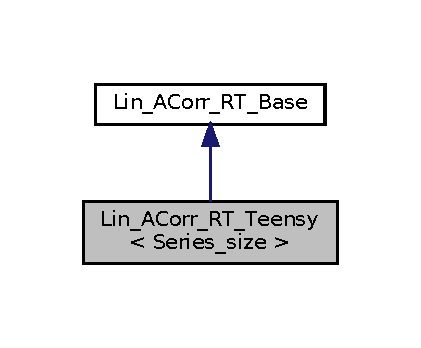
\includegraphics[width=202pt]{classLin__ACorr__RT__Teensy__inherit__graph}
\end{center}
\end{figure}


Collaboration diagram for Lin\+\_\+\+A\+Corr\+\_\+\+R\+T\+\_\+\+Teensy$<$ Series\+\_\+size $>$\+:
\nopagebreak
\begin{figure}[H]
\begin{center}
\leavevmode
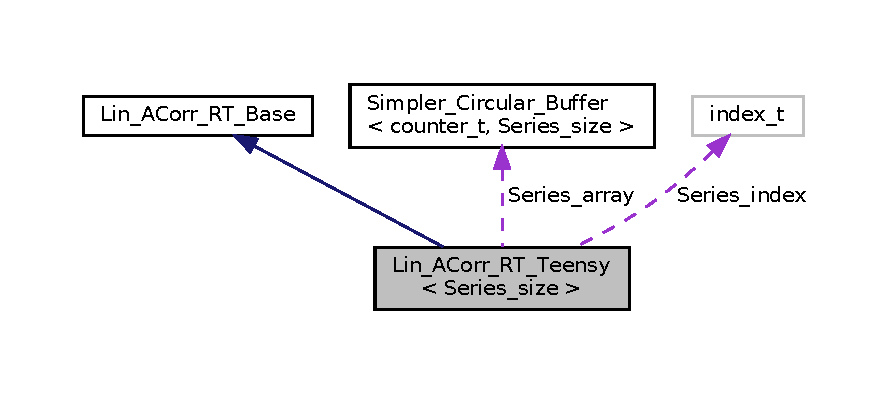
\includegraphics[width=350pt]{classLin__ACorr__RT__Teensy__coll__graph}
\end{center}
\end{figure}
\subsection*{Public Member Functions}
\begin{DoxyCompactItemize}
\item 
void \hyperlink{classLin__ACorr__RT__Teensy_ac07a3acf4e259aee8e5379b0dd327b6c}{\+\_\+\+\_\+attribute\+\_\+\+\_\+} ((flatten)) \hyperlink{classLin__ACorr__RT__Base_a398167525faf2a65f29722e943a0c57e}{push\+\_\+datum}(\hyperlink{types_8hpp_ac89ac912f524b3e3fa3720ea55fec966}{counter\+\_\+t} datum) override
\begin{DoxyCompactList}\small\item\em Stores the last active index → Post-\/increment. \end{DoxyCompactList}\item 
void \hyperlink{classLin__ACorr__RT__Teensy_a0bfee7278e28c759cca2497749aeecf7}{\+\_\+\+\_\+attribute\+\_\+\+\_\+} ((flatten)) \hyperlink{classLin__ACorr__RT__Base_a91c95a49619995f40aeae80916afed3e}{push\+\_\+data}(const \hyperlink{types_8hpp_ac89ac912f524b3e3fa3720ea55fec966}{counter\+\_\+t} $\ast$container
\end{DoxyCompactItemize}
\subsection*{Public Attributes}
\begin{DoxyCompactItemize}
\item 
\hyperlink{types_8hpp_ac89ac912f524b3e3fa3720ea55fec966}{counter\+\_\+t} \hyperlink{classLin__ACorr__RT__Teensy_af4dda93e07198bae54553a8f11773e74}{Channel\+\_\+array} \mbox{[}Series\+\_\+size\mbox{]} = \{0\}
\item 
\hyperlink{classSimpler__Circular__Buffer}{Simpler\+\_\+\+Circular\+\_\+\+Buffer}$<$ \hyperlink{types_8hpp_ac89ac912f524b3e3fa3720ea55fec966}{counter\+\_\+t}, Series\+\_\+size $>$ \hyperlink{classLin__ACorr__RT__Teensy_a9a619d1a74076f0bac8b7f03acebbb75}{Series\+\_\+array}
\begin{DoxyCompactList}\small\item\em Stores the Channel output. \end{DoxyCompactList}\item 
\hyperlink{types_8hpp_a7c40bb931c31595ed6308605f4537447}{index\+\_\+t} \hyperlink{classLin__ACorr__RT__Teensy_a495539383a4cab5ff611545361600599}{Series\+\_\+index} = 0
\begin{DoxyCompactList}\small\item\em Stores the data points in a circular Buffer. \end{DoxyCompactList}\end{DoxyCompactItemize}


\subsection{Detailed Description}
\subsubsection*{template$<$index\+\_\+t Series\+\_\+size$>$\newline
class Lin\+\_\+\+A\+Corr\+\_\+\+R\+T\+\_\+\+Teensy$<$ Series\+\_\+size $>$}

This is an implementation of \hyperlink{classLin__ACorr__RT__Base}{Lin\+\_\+\+A\+Corr\+\_\+\+R\+T\+\_\+\+Base} for Teensy with {\bfseries }(No normalisation or baseline subtraction.) 

\begin{DoxyNote}{Note}
\{ Template parameter -\/ Size of the Series and Channel array and indicates the maximum points that can be stored by the correlator object. The circuular buffer will then rewrite the older points to accomodate for the other points. \} 
\end{DoxyNote}


\subsection{Member Function Documentation}
\mbox{\Hypertarget{classLin__ACorr__RT__Teensy_ac07a3acf4e259aee8e5379b0dd327b6c}\label{classLin__ACorr__RT__Teensy_ac07a3acf4e259aee8e5379b0dd327b6c}} 
\index{Lin\+\_\+\+A\+Corr\+\_\+\+R\+T\+\_\+\+Teensy@{Lin\+\_\+\+A\+Corr\+\_\+\+R\+T\+\_\+\+Teensy}!\+\_\+\+\_\+attribute\+\_\+\+\_\+@{\+\_\+\+\_\+attribute\+\_\+\+\_\+}}
\index{\+\_\+\+\_\+attribute\+\_\+\+\_\+@{\+\_\+\+\_\+attribute\+\_\+\+\_\+}!Lin\+\_\+\+A\+Corr\+\_\+\+R\+T\+\_\+\+Teensy@{Lin\+\_\+\+A\+Corr\+\_\+\+R\+T\+\_\+\+Teensy}}
\subsubsection{\texorpdfstring{\+\_\+\+\_\+attribute\+\_\+\+\_\+()}{\_\_attribute\_\_()}\hspace{0.1cm}{\footnotesize\ttfamily [1/2]}}
{\footnotesize\ttfamily template$<$index\+\_\+t Series\+\_\+size$>$ \\
void \hyperlink{classLin__ACorr__RT__Teensy}{Lin\+\_\+\+A\+Corr\+\_\+\+R\+T\+\_\+\+Teensy}$<$ Series\+\_\+size $>$\+::\+\_\+\+\_\+attribute\+\_\+\+\_\+ (\begin{DoxyParamCaption}\item[{(flatten)}]{ }\end{DoxyParamCaption})\hspace{0.3cm}{\ttfamily [inline]}, {\ttfamily [override]}}



Stores the last active index → Post-\/increment. 

\mbox{\Hypertarget{classLin__ACorr__RT__Teensy_a0bfee7278e28c759cca2497749aeecf7}\label{classLin__ACorr__RT__Teensy_a0bfee7278e28c759cca2497749aeecf7}} 
\index{Lin\+\_\+\+A\+Corr\+\_\+\+R\+T\+\_\+\+Teensy@{Lin\+\_\+\+A\+Corr\+\_\+\+R\+T\+\_\+\+Teensy}!\+\_\+\+\_\+attribute\+\_\+\+\_\+@{\+\_\+\+\_\+attribute\+\_\+\+\_\+}}
\index{\+\_\+\+\_\+attribute\+\_\+\+\_\+@{\+\_\+\+\_\+attribute\+\_\+\+\_\+}!Lin\+\_\+\+A\+Corr\+\_\+\+R\+T\+\_\+\+Teensy@{Lin\+\_\+\+A\+Corr\+\_\+\+R\+T\+\_\+\+Teensy}}
\subsubsection{\texorpdfstring{\+\_\+\+\_\+attribute\+\_\+\+\_\+()}{\_\_attribute\_\_()}\hspace{0.1cm}{\footnotesize\ttfamily [2/2]}}
{\footnotesize\ttfamily template$<$index\+\_\+t Series\+\_\+size$>$ \\
void \hyperlink{classLin__ACorr__RT__Teensy}{Lin\+\_\+\+A\+Corr\+\_\+\+R\+T\+\_\+\+Teensy}$<$ Series\+\_\+size $>$\+::\+\_\+\+\_\+attribute\+\_\+\+\_\+ (\begin{DoxyParamCaption}\item[{(flatten)}]{ }\end{DoxyParamCaption}) const}



\subsection{Member Data Documentation}
\mbox{\Hypertarget{classLin__ACorr__RT__Teensy_af4dda93e07198bae54553a8f11773e74}\label{classLin__ACorr__RT__Teensy_af4dda93e07198bae54553a8f11773e74}} 
\index{Lin\+\_\+\+A\+Corr\+\_\+\+R\+T\+\_\+\+Teensy@{Lin\+\_\+\+A\+Corr\+\_\+\+R\+T\+\_\+\+Teensy}!Channel\+\_\+array@{Channel\+\_\+array}}
\index{Channel\+\_\+array@{Channel\+\_\+array}!Lin\+\_\+\+A\+Corr\+\_\+\+R\+T\+\_\+\+Teensy@{Lin\+\_\+\+A\+Corr\+\_\+\+R\+T\+\_\+\+Teensy}}
\subsubsection{\texorpdfstring{Channel\+\_\+array}{Channel\_array}}
{\footnotesize\ttfamily template$<$index\+\_\+t Series\+\_\+size$>$ \\
\hyperlink{types_8hpp_ac89ac912f524b3e3fa3720ea55fec966}{counter\+\_\+t} \hyperlink{classLin__ACorr__RT__Teensy}{Lin\+\_\+\+A\+Corr\+\_\+\+R\+T\+\_\+\+Teensy}$<$ Series\+\_\+size $>$\+::Channel\+\_\+array\mbox{[}Series\+\_\+size\mbox{]} = \{0\}}

\mbox{\Hypertarget{classLin__ACorr__RT__Teensy_a9a619d1a74076f0bac8b7f03acebbb75}\label{classLin__ACorr__RT__Teensy_a9a619d1a74076f0bac8b7f03acebbb75}} 
\index{Lin\+\_\+\+A\+Corr\+\_\+\+R\+T\+\_\+\+Teensy@{Lin\+\_\+\+A\+Corr\+\_\+\+R\+T\+\_\+\+Teensy}!Series\+\_\+array@{Series\+\_\+array}}
\index{Series\+\_\+array@{Series\+\_\+array}!Lin\+\_\+\+A\+Corr\+\_\+\+R\+T\+\_\+\+Teensy@{Lin\+\_\+\+A\+Corr\+\_\+\+R\+T\+\_\+\+Teensy}}
\subsubsection{\texorpdfstring{Series\+\_\+array}{Series\_array}}
{\footnotesize\ttfamily template$<$index\+\_\+t Series\+\_\+size$>$ \\
\hyperlink{classSimpler__Circular__Buffer}{Simpler\+\_\+\+Circular\+\_\+\+Buffer}$<$\hyperlink{types_8hpp_ac89ac912f524b3e3fa3720ea55fec966}{counter\+\_\+t}, Series\+\_\+size$>$ \hyperlink{classLin__ACorr__RT__Teensy}{Lin\+\_\+\+A\+Corr\+\_\+\+R\+T\+\_\+\+Teensy}$<$ Series\+\_\+size $>$\+::Series\+\_\+array}



Stores the Channel output. 

\mbox{\Hypertarget{classLin__ACorr__RT__Teensy_a495539383a4cab5ff611545361600599}\label{classLin__ACorr__RT__Teensy_a495539383a4cab5ff611545361600599}} 
\index{Lin\+\_\+\+A\+Corr\+\_\+\+R\+T\+\_\+\+Teensy@{Lin\+\_\+\+A\+Corr\+\_\+\+R\+T\+\_\+\+Teensy}!Series\+\_\+index@{Series\+\_\+index}}
\index{Series\+\_\+index@{Series\+\_\+index}!Lin\+\_\+\+A\+Corr\+\_\+\+R\+T\+\_\+\+Teensy@{Lin\+\_\+\+A\+Corr\+\_\+\+R\+T\+\_\+\+Teensy}}
\subsubsection{\texorpdfstring{Series\+\_\+index}{Series\_index}}
{\footnotesize\ttfamily template$<$index\+\_\+t Series\+\_\+size$>$ \\
\hyperlink{types_8hpp_a7c40bb931c31595ed6308605f4537447}{index\+\_\+t} \hyperlink{classLin__ACorr__RT__Teensy}{Lin\+\_\+\+A\+Corr\+\_\+\+R\+T\+\_\+\+Teensy}$<$ Series\+\_\+size $>$\+::Series\+\_\+index = 0}



Stores the data points in a circular Buffer. 



The documentation for this class was generated from the following file\+:\begin{DoxyCompactItemize}
\item 
/mnt/m/code/\+Correlator/\+Software/\hyperlink{Lin__ACorr__RT__Teensy_8hpp}{Lin\+\_\+\+A\+Corr\+\_\+\+R\+T\+\_\+\+Teensy.\+hpp}\end{DoxyCompactItemize}

\hypertarget{classLin__CrossCorr__RT__Base}{}\section{Lin\+\_\+\+Cross\+Corr\+\_\+\+R\+T\+\_\+\+Base Class Reference}
\label{classLin__CrossCorr__RT__Base}\index{Lin\+\_\+\+Cross\+Corr\+\_\+\+R\+T\+\_\+\+Base@{Lin\+\_\+\+Cross\+Corr\+\_\+\+R\+T\+\_\+\+Base}}


This class is a blank interface for all objects that are — {\bfseries \{Linear} Real-\/\+Time Software Auto-\/\+Correlators\}.  




{\ttfamily \#include $<$Lin\+\_\+\+Cross\+Corr\+\_\+\+R\+T\+\_\+\+Base.\+hpp$>$}



Inheritance diagram for Lin\+\_\+\+Cross\+Corr\+\_\+\+R\+T\+\_\+\+Base\+:
\nopagebreak
\begin{figure}[H]
\begin{center}
\leavevmode
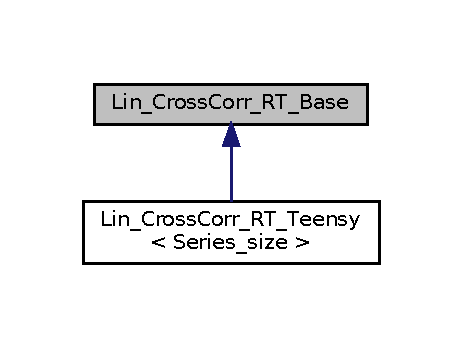
\includegraphics[width=222pt]{classLin__CrossCorr__RT__Base__inherit__graph}
\end{center}
\end{figure}
\subsection*{Public Member Functions}
\begin{DoxyCompactItemize}
\item 
virtual void \hyperlink{classLin__CrossCorr__RT__Base_abdc90b5ab6a5f7ac98e97b3d16261834}{push\+\_\+datum} (\hyperlink{types_8hpp_ac89ac912f524b3e3fa3720ea55fec966}{counter\+\_\+t} datum1, \hyperlink{types_8hpp_ac89ac912f524b3e3fa3720ea55fec966}{counter\+\_\+t} datum2)=0
\begin{DoxyCompactList}\small\item\em Accepts two single {\ttfamily datum} from the counters — which is the lowest order of data aggregate, appends to Series\+\_\+array(s) and updates relevant channels. \end{DoxyCompactList}\item 
virtual void \hyperlink{classLin__CrossCorr__RT__Base_a48faa93c6766605436fd8399949beb11}{push\+\_\+data} (const \hyperlink{types_8hpp_ac89ac912f524b3e3fa3720ea55fec966}{counter\+\_\+t} $\ast$container1, const \hyperlink{types_8hpp_ac89ac912f524b3e3fa3720ea55fec966}{counter\+\_\+t} $\ast$container2, const \hyperlink{types_8hpp_a7c40bb931c31595ed6308605f4537447}{index\+\_\+t} size)=0
\begin{DoxyCompactList}\small\item\em Repeatedy calls {\ttfamily Lin\+\_\+\+Cross\+Corr\+\_\+\+R\+T\+\_\+\+Base\+::push\+\_\+datam()} on all the elements of the countainers. \end{DoxyCompactList}\item 
virtual double \hyperlink{classLin__CrossCorr__RT__Base_a43779bc7fd546fa8f73713de4bd6e285}{norm} (\hyperlink{types_8hpp_a7c40bb931c31595ed6308605f4537447}{index\+\_\+t} lag)=0
\begin{DoxyCompactList}\small\item\em Takes in the lag value and returns the normalization (divider) for the passed lag value. \end{DoxyCompactList}\item 
virtual void \hyperlink{group__Lin__CorrCorr__Base__Out_ga5d7bad992e07606a18ea828aeb768e1f}{ch\+\_\+out} () const =0
\begin{DoxyCompactList}\small\item\em Outputs all the channels using specific implementation based methods. Both the channel outputs are appended together one after the other. 12-\/21. \end{DoxyCompactList}\item 
virtual void \hyperlink{group__Lin__CorrCorr__Base__Out_gaaac0e6901df27096d687c228638c012b}{ch\+\_\+out\+\_\+norm} () const =0
\begin{DoxyCompactList}\small\item\em Outputs all the channels with {\bfseries } $<$normalisation$>$ using specific implementation based methods. \end{DoxyCompactList}\item 
virtual \hyperlink{types_8hpp_ac89ac912f524b3e3fa3720ea55fec966}{counter\+\_\+t} $\ast$ \hyperlink{group__Lin__CorrCorr__Base__Out_gacc777900e8d232740373a70c1d5b4cce}{get\+\_\+ch\+\_\+array12} () const =0
\item 
virtual \hyperlink{types_8hpp_ac89ac912f524b3e3fa3720ea55fec966}{counter\+\_\+t} $\ast$ \hyperlink{group__Lin__CorrCorr__Base__Out_ga9f075c765376a156da279b23bc18c07f}{get\+\_\+ch\+\_\+array21} () const =0
\end{DoxyCompactItemize}


\subsection{Detailed Description}
This class is a blank interface for all objects that are — {\bfseries \{Linear} Real-\/\+Time Software Auto-\/\+Correlators\}. 

\subsection{Member Function Documentation}
\mbox{\Hypertarget{classLin__CrossCorr__RT__Base_a43779bc7fd546fa8f73713de4bd6e285}\label{classLin__CrossCorr__RT__Base_a43779bc7fd546fa8f73713de4bd6e285}} 
\index{Lin\+\_\+\+Cross\+Corr\+\_\+\+R\+T\+\_\+\+Base@{Lin\+\_\+\+Cross\+Corr\+\_\+\+R\+T\+\_\+\+Base}!norm@{norm}}
\index{norm@{norm}!Lin\+\_\+\+Cross\+Corr\+\_\+\+R\+T\+\_\+\+Base@{Lin\+\_\+\+Cross\+Corr\+\_\+\+R\+T\+\_\+\+Base}}
\subsubsection{\texorpdfstring{norm()}{norm()}}
{\footnotesize\ttfamily virtual double Lin\+\_\+\+Cross\+Corr\+\_\+\+R\+T\+\_\+\+Base\+::norm (\begin{DoxyParamCaption}\item[{\hyperlink{types_8hpp_a7c40bb931c31595ed6308605f4537447}{index\+\_\+t}}]{lag }\end{DoxyParamCaption})\hspace{0.3cm}{\ttfamily [inline]}, {\ttfamily [pure virtual]}}



Takes in the lag value and returns the normalization (divider) for the passed lag value. 

\mbox{\Hypertarget{classLin__CrossCorr__RT__Base_a48faa93c6766605436fd8399949beb11}\label{classLin__CrossCorr__RT__Base_a48faa93c6766605436fd8399949beb11}} 
\index{Lin\+\_\+\+Cross\+Corr\+\_\+\+R\+T\+\_\+\+Base@{Lin\+\_\+\+Cross\+Corr\+\_\+\+R\+T\+\_\+\+Base}!push\+\_\+data@{push\+\_\+data}}
\index{push\+\_\+data@{push\+\_\+data}!Lin\+\_\+\+Cross\+Corr\+\_\+\+R\+T\+\_\+\+Base@{Lin\+\_\+\+Cross\+Corr\+\_\+\+R\+T\+\_\+\+Base}}
\subsubsection{\texorpdfstring{push\+\_\+data()}{push\_data()}}
{\footnotesize\ttfamily virtual void Lin\+\_\+\+Cross\+Corr\+\_\+\+R\+T\+\_\+\+Base\+::push\+\_\+data (\begin{DoxyParamCaption}\item[{const \hyperlink{types_8hpp_ac89ac912f524b3e3fa3720ea55fec966}{counter\+\_\+t} $\ast$}]{container1,  }\item[{const \hyperlink{types_8hpp_ac89ac912f524b3e3fa3720ea55fec966}{counter\+\_\+t} $\ast$}]{container2,  }\item[{const \hyperlink{types_8hpp_a7c40bb931c31595ed6308605f4537447}{index\+\_\+t}}]{size }\end{DoxyParamCaption})\hspace{0.3cm}{\ttfamily [inline]}, {\ttfamily [pure virtual]}}



Repeatedy calls {\ttfamily Lin\+\_\+\+Cross\+Corr\+\_\+\+R\+T\+\_\+\+Base\+::push\+\_\+datam()} on all the elements of the countainers. 

\begin{DoxyAttention}{Attention}
The containers must be of the same size. 
\end{DoxyAttention}
\mbox{\Hypertarget{classLin__CrossCorr__RT__Base_abdc90b5ab6a5f7ac98e97b3d16261834}\label{classLin__CrossCorr__RT__Base_abdc90b5ab6a5f7ac98e97b3d16261834}} 
\index{Lin\+\_\+\+Cross\+Corr\+\_\+\+R\+T\+\_\+\+Base@{Lin\+\_\+\+Cross\+Corr\+\_\+\+R\+T\+\_\+\+Base}!push\+\_\+datum@{push\+\_\+datum}}
\index{push\+\_\+datum@{push\+\_\+datum}!Lin\+\_\+\+Cross\+Corr\+\_\+\+R\+T\+\_\+\+Base@{Lin\+\_\+\+Cross\+Corr\+\_\+\+R\+T\+\_\+\+Base}}
\subsubsection{\texorpdfstring{push\+\_\+datum()}{push\_datum()}}
{\footnotesize\ttfamily virtual void Lin\+\_\+\+Cross\+Corr\+\_\+\+R\+T\+\_\+\+Base\+::push\+\_\+datum (\begin{DoxyParamCaption}\item[{\hyperlink{types_8hpp_ac89ac912f524b3e3fa3720ea55fec966}{counter\+\_\+t}}]{datum1,  }\item[{\hyperlink{types_8hpp_ac89ac912f524b3e3fa3720ea55fec966}{counter\+\_\+t}}]{datum2 }\end{DoxyParamCaption})\hspace{0.3cm}{\ttfamily [inline]}, {\ttfamily [pure virtual]}}



Accepts two single {\ttfamily datum} from the counters — which is the lowest order of data aggregate, appends to Series\+\_\+array(s) and updates relevant channels. 



The documentation for this class was generated from the following file\+:\begin{DoxyCompactItemize}
\item 
/mnt/m/code/\+Correlator/\+Software/\hyperlink{Lin__CrossCorr__RT__Base_8hpp}{Lin\+\_\+\+Cross\+Corr\+\_\+\+R\+T\+\_\+\+Base.\+hpp}\end{DoxyCompactItemize}

\hypertarget{classLin__CrossCorr__RT__Teensy}{}\section{Lin\+\_\+\+Cross\+Corr\+\_\+\+R\+T\+\_\+\+Teensy$<$ Series\+\_\+size $>$ Class Template Reference}
\label{classLin__CrossCorr__RT__Teensy}\index{Lin\+\_\+\+Cross\+Corr\+\_\+\+R\+T\+\_\+\+Teensy$<$ Series\+\_\+size $>$@{Lin\+\_\+\+Cross\+Corr\+\_\+\+R\+T\+\_\+\+Teensy$<$ Series\+\_\+size $>$}}


This is an implementation of Lin\+\_\+\+A\+Corr\+\_\+\+R\+T\+\_\+\+Base for Teensy with {\bfseries }(No normalisation or baseline subtraction.)  




{\ttfamily \#include $<$Lin\+\_\+\+Cross\+Corr\+\_\+\+R\+T\+\_\+\+Teensy.\+hpp$>$}



Inheritance diagram for Lin\+\_\+\+Cross\+Corr\+\_\+\+R\+T\+\_\+\+Teensy$<$ Series\+\_\+size $>$\+:\nopagebreak
\begin{figure}[H]
\begin{center}
\leavevmode
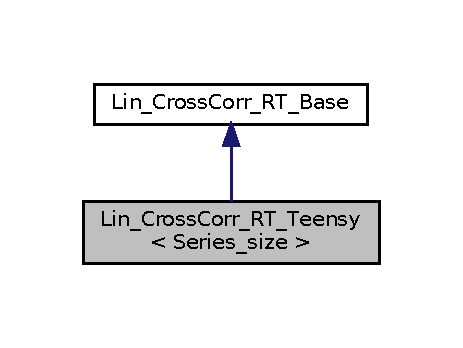
\includegraphics[width=222pt]{classLin__CrossCorr__RT__Teensy__inherit__graph}
\end{center}
\end{figure}


Collaboration diagram for Lin\+\_\+\+Cross\+Corr\+\_\+\+R\+T\+\_\+\+Teensy$<$ Series\+\_\+size $>$\+:\nopagebreak
\begin{figure}[H]
\begin{center}
\leavevmode
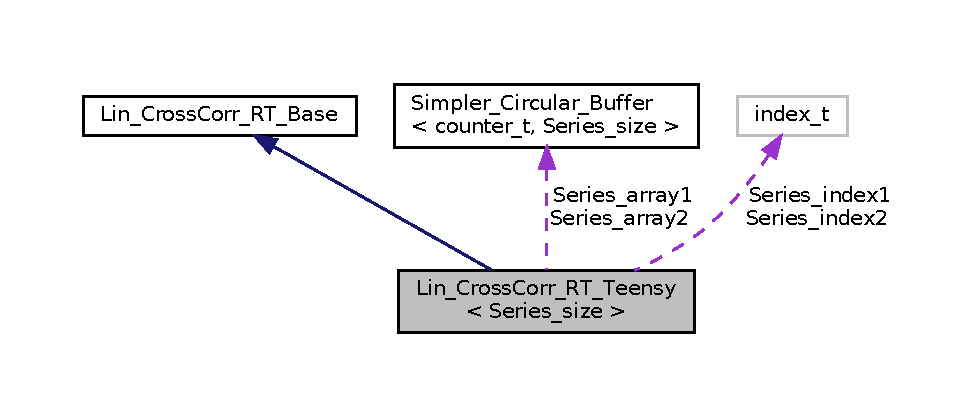
\includegraphics[width=350pt]{classLin__CrossCorr__RT__Teensy__coll__graph}
\end{center}
\end{figure}
\subsection*{Public Member Functions}
\begin{DoxyCompactItemize}
\item 
void \hyperlink{classLin__CrossCorr__RT__Teensy_a33f639fa3a6f025d5a9ebe60b969cc55}{\+\_\+\+\_\+attribute\+\_\+\+\_\+} ((flatten)) push\+\_\+datum(\hyperlink{types_8hpp_a22f279793847eba127de149437848c48}{counter\+\_\+t} datum1
\begin{DoxyCompactList}\small\item\em Stores the last active index → Post-\/increment. \end{DoxyCompactList}\item 
\hyperlink{classLin__CrossCorr__RT__Teensy_a509bcfdab5a3239a014f5805c388172a}{Series\+\_\+array2} \hyperlink{classLin__CrossCorr__RT__Teensy_af39e68107a612ca22a83046b10f52afb}{push\+\_\+back} (datum2)
\item 
\hyperlink{classLin__CrossCorr__RT__Teensy_aca7ed016d12272211206139cd120b359}{for} (unsigned int i=0;i$<$=Series\+\_\+size;i++)
\item 
void \hyperlink{classLin__CrossCorr__RT__Teensy_a1d3a4042f89c99d3705f50666fa7735c}{\+\_\+\+\_\+attribute\+\_\+\+\_\+} ((flatten)) push\+\_\+data(const \hyperlink{types_8hpp_a22f279793847eba127de149437848c48}{counter\+\_\+t} $\ast$container1
\end{DoxyCompactItemize}
\subsection*{Public Attributes}
\begin{DoxyCompactItemize}
\item 
\hyperlink{types_8hpp_a22f279793847eba127de149437848c48}{counter\+\_\+t} \hyperlink{classLin__CrossCorr__RT__Teensy_ad1a3471c7cbcee3bd9b800571cd2ae3d}{Channel\+\_\+array12} \mbox{[}Series\+\_\+size\mbox{]} = \{0\}
\item 
\hyperlink{types_8hpp_a22f279793847eba127de149437848c48}{counter\+\_\+t} \hyperlink{classLin__CrossCorr__RT__Teensy_a03a339977779908684cba60c8d3f9738}{Channel\+\_\+array21} \mbox{[}Series\+\_\+size\mbox{]} = \{0\}
\begin{DoxyCompactList}\small\item\em Stores the Channel output -\/ 12. \end{DoxyCompactList}\item 
\hyperlink{classSimpler__Circular__Buffer}{Simpler\+\_\+\+Circular\+\_\+\+Buffer}$<$ \hyperlink{types_8hpp_a22f279793847eba127de149437848c48}{counter\+\_\+t}, Series\+\_\+size $>$ \hyperlink{classLin__CrossCorr__RT__Teensy_a13307ad04080703e9ef8c0cd9794a6b0}{Series\+\_\+array1}
\begin{DoxyCompactList}\small\item\em Stores the Channel output -\/ 21. \end{DoxyCompactList}\item 
\hyperlink{classSimpler__Circular__Buffer}{Simpler\+\_\+\+Circular\+\_\+\+Buffer}$<$ \hyperlink{types_8hpp_a22f279793847eba127de149437848c48}{counter\+\_\+t}, Series\+\_\+size $>$ \hyperlink{classLin__CrossCorr__RT__Teensy_a509bcfdab5a3239a014f5805c388172a}{Series\+\_\+array2}
\item 
\hyperlink{types_8hpp_ab41b824af8e088d090c0b9e60f536c9d}{index\+\_\+t} \hyperlink{classLin__CrossCorr__RT__Teensy_afcf9512277d8bd2183ae44b8da1096df}{Series\+\_\+index1} = 0
\item 
\hyperlink{types_8hpp_ab41b824af8e088d090c0b9e60f536c9d}{index\+\_\+t} \hyperlink{classLin__CrossCorr__RT__Teensy_a945eda00978a28dd536e58e225821af6}{Series\+\_\+index2} = 0
\begin{DoxyCompactList}\small\item\em Stores the last active index → Post-\/increment. \end{DoxyCompactList}\item 
void \hyperlink{types_8hpp_a22f279793847eba127de149437848c48}{counter\+\_\+t} datum2 \hyperlink{classLin__CrossCorr__RT__Teensy_a5baab98aab70338799de9f82e7c7cc06}{override}
\item 
\hyperlink{classLin__CrossCorr__RT__Teensy_abefa188b0d61b97e915849fa8d11cc9f}{Series\+\_\+index1}
\item 
\hyperlink{classLin__CrossCorr__RT__Teensy_a4f84a456a7d6e90e8676e4c5ed059776}{Series\+\_\+index2}
\item 
void const \hyperlink{types_8hpp_a22f279793847eba127de149437848c48}{counter\+\_\+t} $\ast$ \hyperlink{classLin__CrossCorr__RT__Teensy_a9c49e09d3817e1f1344c51928e3afb57}{container2}
\end{DoxyCompactItemize}


\subsection{Detailed Description}
\subsubsection*{template$<$index\+\_\+t Series\+\_\+size$>$\newline
class Lin\+\_\+\+Cross\+Corr\+\_\+\+R\+T\+\_\+\+Teensy$<$ Series\+\_\+size $>$}

This is an implementation of Lin\+\_\+\+A\+Corr\+\_\+\+R\+T\+\_\+\+Base for Teensy with {\bfseries }(No normalisation or baseline subtraction.) 

\begin{DoxyNote}{Note}
\{ Template parameter -\/ Size of the Series and Channel array and indicates the maximum points that can be stored by the correlator object. The circuular buffer will then rewrite the older points to accomodate for the other points. \} 
\end{DoxyNote}


\subsection{Member Function Documentation}
\mbox{\Hypertarget{classLin__CrossCorr__RT__Teensy_a33f639fa3a6f025d5a9ebe60b969cc55}\label{classLin__CrossCorr__RT__Teensy_a33f639fa3a6f025d5a9ebe60b969cc55}} 
\index{Lin\+\_\+\+Cross\+Corr\+\_\+\+R\+T\+\_\+\+Teensy@{Lin\+\_\+\+Cross\+Corr\+\_\+\+R\+T\+\_\+\+Teensy}!\+\_\+\+\_\+attribute\+\_\+\+\_\+@{\+\_\+\+\_\+attribute\+\_\+\+\_\+}}
\index{\+\_\+\+\_\+attribute\+\_\+\+\_\+@{\+\_\+\+\_\+attribute\+\_\+\+\_\+}!Lin\+\_\+\+Cross\+Corr\+\_\+\+R\+T\+\_\+\+Teensy@{Lin\+\_\+\+Cross\+Corr\+\_\+\+R\+T\+\_\+\+Teensy}}
\subsubsection{\texorpdfstring{\+\_\+\+\_\+attribute\+\_\+\+\_\+()}{\_\_attribute\_\_()}\hspace{0.1cm}{\footnotesize\ttfamily [1/2]}}
{\footnotesize\ttfamily template$<$index\+\_\+t Series\+\_\+size$>$ \\
void \hyperlink{classLin__CrossCorr__RT__Teensy}{Lin\+\_\+\+Cross\+Corr\+\_\+\+R\+T\+\_\+\+Teensy}$<$ Series\+\_\+size $>$\+::\+\_\+\+\_\+attribute\+\_\+\+\_\+ (\begin{DoxyParamCaption}\item[{(flatten)}]{ }\end{DoxyParamCaption})}



Stores the last active index → Post-\/increment. 

\mbox{\Hypertarget{classLin__CrossCorr__RT__Teensy_a1d3a4042f89c99d3705f50666fa7735c}\label{classLin__CrossCorr__RT__Teensy_a1d3a4042f89c99d3705f50666fa7735c}} 
\index{Lin\+\_\+\+Cross\+Corr\+\_\+\+R\+T\+\_\+\+Teensy@{Lin\+\_\+\+Cross\+Corr\+\_\+\+R\+T\+\_\+\+Teensy}!\+\_\+\+\_\+attribute\+\_\+\+\_\+@{\+\_\+\+\_\+attribute\+\_\+\+\_\+}}
\index{\+\_\+\+\_\+attribute\+\_\+\+\_\+@{\+\_\+\+\_\+attribute\+\_\+\+\_\+}!Lin\+\_\+\+Cross\+Corr\+\_\+\+R\+T\+\_\+\+Teensy@{Lin\+\_\+\+Cross\+Corr\+\_\+\+R\+T\+\_\+\+Teensy}}
\subsubsection{\texorpdfstring{\+\_\+\+\_\+attribute\+\_\+\+\_\+()}{\_\_attribute\_\_()}\hspace{0.1cm}{\footnotesize\ttfamily [2/2]}}
{\footnotesize\ttfamily template$<$index\+\_\+t Series\+\_\+size$>$ \\
void \hyperlink{classLin__CrossCorr__RT__Teensy}{Lin\+\_\+\+Cross\+Corr\+\_\+\+R\+T\+\_\+\+Teensy}$<$ Series\+\_\+size $>$\+::\+\_\+\+\_\+attribute\+\_\+\+\_\+ (\begin{DoxyParamCaption}\item[{(flatten)}]{ }\end{DoxyParamCaption}) const}

\mbox{\Hypertarget{classLin__CrossCorr__RT__Teensy_aca7ed016d12272211206139cd120b359}\label{classLin__CrossCorr__RT__Teensy_aca7ed016d12272211206139cd120b359}} 
\index{Lin\+\_\+\+Cross\+Corr\+\_\+\+R\+T\+\_\+\+Teensy@{Lin\+\_\+\+Cross\+Corr\+\_\+\+R\+T\+\_\+\+Teensy}!for@{for}}
\index{for@{for}!Lin\+\_\+\+Cross\+Corr\+\_\+\+R\+T\+\_\+\+Teensy@{Lin\+\_\+\+Cross\+Corr\+\_\+\+R\+T\+\_\+\+Teensy}}
\subsubsection{\texorpdfstring{for()}{for()}}
{\footnotesize\ttfamily template$<$index\+\_\+t Series\+\_\+size$>$ \\
\hyperlink{classLin__CrossCorr__RT__Teensy}{Lin\+\_\+\+Cross\+Corr\+\_\+\+R\+T\+\_\+\+Teensy}$<$ Series\+\_\+size $>$\+::for (\begin{DoxyParamCaption}\item[{unsigned int}]{i = {\ttfamily 0;~i~$<$=~Series\+\_\+size;~i++} }\end{DoxyParamCaption})\hspace{0.3cm}{\ttfamily [inline]}}

\mbox{\Hypertarget{classLin__CrossCorr__RT__Teensy_af39e68107a612ca22a83046b10f52afb}\label{classLin__CrossCorr__RT__Teensy_af39e68107a612ca22a83046b10f52afb}} 
\index{Lin\+\_\+\+Cross\+Corr\+\_\+\+R\+T\+\_\+\+Teensy@{Lin\+\_\+\+Cross\+Corr\+\_\+\+R\+T\+\_\+\+Teensy}!push\+\_\+back@{push\+\_\+back}}
\index{push\+\_\+back@{push\+\_\+back}!Lin\+\_\+\+Cross\+Corr\+\_\+\+R\+T\+\_\+\+Teensy@{Lin\+\_\+\+Cross\+Corr\+\_\+\+R\+T\+\_\+\+Teensy}}
\subsubsection{\texorpdfstring{push\+\_\+back()}{push\_back()}}
{\footnotesize\ttfamily template$<$index\+\_\+t Series\+\_\+size$>$ \\
\hyperlink{classLin__CrossCorr__RT__Teensy_a509bcfdab5a3239a014f5805c388172a}{Series\+\_\+array2} \hyperlink{classLin__CrossCorr__RT__Teensy}{Lin\+\_\+\+Cross\+Corr\+\_\+\+R\+T\+\_\+\+Teensy}$<$ Series\+\_\+size $>$\+::push\+\_\+back (\begin{DoxyParamCaption}\item[{datum2}]{ }\end{DoxyParamCaption})}



\subsection{Member Data Documentation}
\mbox{\Hypertarget{classLin__CrossCorr__RT__Teensy_ad1a3471c7cbcee3bd9b800571cd2ae3d}\label{classLin__CrossCorr__RT__Teensy_ad1a3471c7cbcee3bd9b800571cd2ae3d}} 
\index{Lin\+\_\+\+Cross\+Corr\+\_\+\+R\+T\+\_\+\+Teensy@{Lin\+\_\+\+Cross\+Corr\+\_\+\+R\+T\+\_\+\+Teensy}!Channel\+\_\+array12@{Channel\+\_\+array12}}
\index{Channel\+\_\+array12@{Channel\+\_\+array12}!Lin\+\_\+\+Cross\+Corr\+\_\+\+R\+T\+\_\+\+Teensy@{Lin\+\_\+\+Cross\+Corr\+\_\+\+R\+T\+\_\+\+Teensy}}
\subsubsection{\texorpdfstring{Channel\+\_\+array12}{Channel\_array12}}
{\footnotesize\ttfamily template$<$index\+\_\+t Series\+\_\+size$>$ \\
\hyperlink{types_8hpp_a22f279793847eba127de149437848c48}{counter\+\_\+t} \hyperlink{classLin__CrossCorr__RT__Teensy}{Lin\+\_\+\+Cross\+Corr\+\_\+\+R\+T\+\_\+\+Teensy}$<$ Series\+\_\+size $>$\+::Channel\+\_\+array12\mbox{[}Series\+\_\+size\mbox{]} = \{0\}}

\mbox{\Hypertarget{classLin__CrossCorr__RT__Teensy_a03a339977779908684cba60c8d3f9738}\label{classLin__CrossCorr__RT__Teensy_a03a339977779908684cba60c8d3f9738}} 
\index{Lin\+\_\+\+Cross\+Corr\+\_\+\+R\+T\+\_\+\+Teensy@{Lin\+\_\+\+Cross\+Corr\+\_\+\+R\+T\+\_\+\+Teensy}!Channel\+\_\+array21@{Channel\+\_\+array21}}
\index{Channel\+\_\+array21@{Channel\+\_\+array21}!Lin\+\_\+\+Cross\+Corr\+\_\+\+R\+T\+\_\+\+Teensy@{Lin\+\_\+\+Cross\+Corr\+\_\+\+R\+T\+\_\+\+Teensy}}
\subsubsection{\texorpdfstring{Channel\+\_\+array21}{Channel\_array21}}
{\footnotesize\ttfamily template$<$index\+\_\+t Series\+\_\+size$>$ \\
\hyperlink{types_8hpp_a22f279793847eba127de149437848c48}{counter\+\_\+t} \hyperlink{classLin__CrossCorr__RT__Teensy}{Lin\+\_\+\+Cross\+Corr\+\_\+\+R\+T\+\_\+\+Teensy}$<$ Series\+\_\+size $>$\+::Channel\+\_\+array21\mbox{[}Series\+\_\+size\mbox{]} = \{0\}}



Stores the Channel output -\/ 12. 

\mbox{\Hypertarget{classLin__CrossCorr__RT__Teensy_a9c49e09d3817e1f1344c51928e3afb57}\label{classLin__CrossCorr__RT__Teensy_a9c49e09d3817e1f1344c51928e3afb57}} 
\index{Lin\+\_\+\+Cross\+Corr\+\_\+\+R\+T\+\_\+\+Teensy@{Lin\+\_\+\+Cross\+Corr\+\_\+\+R\+T\+\_\+\+Teensy}!container2@{container2}}
\index{container2@{container2}!Lin\+\_\+\+Cross\+Corr\+\_\+\+R\+T\+\_\+\+Teensy@{Lin\+\_\+\+Cross\+Corr\+\_\+\+R\+T\+\_\+\+Teensy}}
\subsubsection{\texorpdfstring{container2}{container2}}
{\footnotesize\ttfamily template$<$index\+\_\+t Series\+\_\+size$>$ \\
void const \hyperlink{types_8hpp_a22f279793847eba127de149437848c48}{counter\+\_\+t}$\ast$ \hyperlink{classLin__CrossCorr__RT__Teensy}{Lin\+\_\+\+Cross\+Corr\+\_\+\+R\+T\+\_\+\+Teensy}$<$ Series\+\_\+size $>$\+::container2}

\mbox{\Hypertarget{classLin__CrossCorr__RT__Teensy_a5baab98aab70338799de9f82e7c7cc06}\label{classLin__CrossCorr__RT__Teensy_a5baab98aab70338799de9f82e7c7cc06}} 
\index{Lin\+\_\+\+Cross\+Corr\+\_\+\+R\+T\+\_\+\+Teensy@{Lin\+\_\+\+Cross\+Corr\+\_\+\+R\+T\+\_\+\+Teensy}!override@{override}}
\index{override@{override}!Lin\+\_\+\+Cross\+Corr\+\_\+\+R\+T\+\_\+\+Teensy@{Lin\+\_\+\+Cross\+Corr\+\_\+\+R\+T\+\_\+\+Teensy}}
\subsubsection{\texorpdfstring{override}{override}}
{\footnotesize\ttfamily template$<$index\+\_\+t Series\+\_\+size$>$ \\
void \hyperlink{types_8hpp_a22f279793847eba127de149437848c48}{counter\+\_\+t} datum2 \hyperlink{classLin__CrossCorr__RT__Teensy}{Lin\+\_\+\+Cross\+Corr\+\_\+\+R\+T\+\_\+\+Teensy}$<$ Series\+\_\+size $>$\+::override}

{\bfseries Initial value\+:}
\begin{DoxyCode}
\{
    \hyperlink{classLin__CrossCorr__RT__Teensy_a13307ad04080703e9ef8c0cd9794a6b0}{Series\_array1}.\hyperlink{classSimpler__Circular__Buffer_af4bdd0a6d3fc7a8c06f62b0d996158f0}{push\_back}(datum1)
\end{DoxyCode}
\mbox{\Hypertarget{classLin__CrossCorr__RT__Teensy_a13307ad04080703e9ef8c0cd9794a6b0}\label{classLin__CrossCorr__RT__Teensy_a13307ad04080703e9ef8c0cd9794a6b0}} 
\index{Lin\+\_\+\+Cross\+Corr\+\_\+\+R\+T\+\_\+\+Teensy@{Lin\+\_\+\+Cross\+Corr\+\_\+\+R\+T\+\_\+\+Teensy}!Series\+\_\+array1@{Series\+\_\+array1}}
\index{Series\+\_\+array1@{Series\+\_\+array1}!Lin\+\_\+\+Cross\+Corr\+\_\+\+R\+T\+\_\+\+Teensy@{Lin\+\_\+\+Cross\+Corr\+\_\+\+R\+T\+\_\+\+Teensy}}
\subsubsection{\texorpdfstring{Series\+\_\+array1}{Series\_array1}}
{\footnotesize\ttfamily template$<$index\+\_\+t Series\+\_\+size$>$ \\
\hyperlink{classSimpler__Circular__Buffer}{Simpler\+\_\+\+Circular\+\_\+\+Buffer}$<$\hyperlink{types_8hpp_a22f279793847eba127de149437848c48}{counter\+\_\+t}, Series\+\_\+size$>$ \hyperlink{classLin__CrossCorr__RT__Teensy}{Lin\+\_\+\+Cross\+Corr\+\_\+\+R\+T\+\_\+\+Teensy}$<$ Series\+\_\+size $>$\+::Series\+\_\+array1}



Stores the Channel output -\/ 21. 

Stores the data points in a circular Buffer \mbox{\Hypertarget{classLin__CrossCorr__RT__Teensy_a509bcfdab5a3239a014f5805c388172a}\label{classLin__CrossCorr__RT__Teensy_a509bcfdab5a3239a014f5805c388172a}} 
\index{Lin\+\_\+\+Cross\+Corr\+\_\+\+R\+T\+\_\+\+Teensy@{Lin\+\_\+\+Cross\+Corr\+\_\+\+R\+T\+\_\+\+Teensy}!Series\+\_\+array2@{Series\+\_\+array2}}
\index{Series\+\_\+array2@{Series\+\_\+array2}!Lin\+\_\+\+Cross\+Corr\+\_\+\+R\+T\+\_\+\+Teensy@{Lin\+\_\+\+Cross\+Corr\+\_\+\+R\+T\+\_\+\+Teensy}}
\subsubsection{\texorpdfstring{Series\+\_\+array2}{Series\_array2}}
{\footnotesize\ttfamily template$<$index\+\_\+t Series\+\_\+size$>$ \\
\hyperlink{classSimpler__Circular__Buffer}{Simpler\+\_\+\+Circular\+\_\+\+Buffer}$<$\hyperlink{types_8hpp_a22f279793847eba127de149437848c48}{counter\+\_\+t}, Series\+\_\+size$>$ \hyperlink{classLin__CrossCorr__RT__Teensy}{Lin\+\_\+\+Cross\+Corr\+\_\+\+R\+T\+\_\+\+Teensy}$<$ Series\+\_\+size $>$\+::Series\+\_\+array2}

\mbox{\Hypertarget{classLin__CrossCorr__RT__Teensy_afcf9512277d8bd2183ae44b8da1096df}\label{classLin__CrossCorr__RT__Teensy_afcf9512277d8bd2183ae44b8da1096df}} 
\index{Lin\+\_\+\+Cross\+Corr\+\_\+\+R\+T\+\_\+\+Teensy@{Lin\+\_\+\+Cross\+Corr\+\_\+\+R\+T\+\_\+\+Teensy}!Series\+\_\+index1@{Series\+\_\+index1}}
\index{Series\+\_\+index1@{Series\+\_\+index1}!Lin\+\_\+\+Cross\+Corr\+\_\+\+R\+T\+\_\+\+Teensy@{Lin\+\_\+\+Cross\+Corr\+\_\+\+R\+T\+\_\+\+Teensy}}
\subsubsection{\texorpdfstring{Series\+\_\+index1}{Series\_index1}\hspace{0.1cm}{\footnotesize\ttfamily [1/2]}}
{\footnotesize\ttfamily template$<$index\+\_\+t Series\+\_\+size$>$ \\
\hyperlink{types_8hpp_ab41b824af8e088d090c0b9e60f536c9d}{index\+\_\+t} \hyperlink{classLin__CrossCorr__RT__Teensy}{Lin\+\_\+\+Cross\+Corr\+\_\+\+R\+T\+\_\+\+Teensy}$<$ Series\+\_\+size $>$\+::Series\+\_\+index1 = 0}

\mbox{\Hypertarget{classLin__CrossCorr__RT__Teensy_abefa188b0d61b97e915849fa8d11cc9f}\label{classLin__CrossCorr__RT__Teensy_abefa188b0d61b97e915849fa8d11cc9f}} 
\index{Lin\+\_\+\+Cross\+Corr\+\_\+\+R\+T\+\_\+\+Teensy@{Lin\+\_\+\+Cross\+Corr\+\_\+\+R\+T\+\_\+\+Teensy}!Series\+\_\+index1@{Series\+\_\+index1}}
\index{Series\+\_\+index1@{Series\+\_\+index1}!Lin\+\_\+\+Cross\+Corr\+\_\+\+R\+T\+\_\+\+Teensy@{Lin\+\_\+\+Cross\+Corr\+\_\+\+R\+T\+\_\+\+Teensy}}
\subsubsection{\texorpdfstring{Series\+\_\+index1}{Series\_index1}\hspace{0.1cm}{\footnotesize\ttfamily [2/2]}}
{\footnotesize\ttfamily template$<$index\+\_\+t Series\+\_\+size$>$ \\
\hyperlink{classLin__CrossCorr__RT__Teensy}{Lin\+\_\+\+Cross\+Corr\+\_\+\+R\+T\+\_\+\+Teensy}$<$ Series\+\_\+size $>$\+::Series\+\_\+index1}

\mbox{\Hypertarget{classLin__CrossCorr__RT__Teensy_a945eda00978a28dd536e58e225821af6}\label{classLin__CrossCorr__RT__Teensy_a945eda00978a28dd536e58e225821af6}} 
\index{Lin\+\_\+\+Cross\+Corr\+\_\+\+R\+T\+\_\+\+Teensy@{Lin\+\_\+\+Cross\+Corr\+\_\+\+R\+T\+\_\+\+Teensy}!Series\+\_\+index2@{Series\+\_\+index2}}
\index{Series\+\_\+index2@{Series\+\_\+index2}!Lin\+\_\+\+Cross\+Corr\+\_\+\+R\+T\+\_\+\+Teensy@{Lin\+\_\+\+Cross\+Corr\+\_\+\+R\+T\+\_\+\+Teensy}}
\subsubsection{\texorpdfstring{Series\+\_\+index2}{Series\_index2}\hspace{0.1cm}{\footnotesize\ttfamily [1/2]}}
{\footnotesize\ttfamily template$<$index\+\_\+t Series\+\_\+size$>$ \\
\hyperlink{types_8hpp_ab41b824af8e088d090c0b9e60f536c9d}{index\+\_\+t} \hyperlink{classLin__CrossCorr__RT__Teensy}{Lin\+\_\+\+Cross\+Corr\+\_\+\+R\+T\+\_\+\+Teensy}$<$ Series\+\_\+size $>$\+::Series\+\_\+index2 = 0}



Stores the last active index → Post-\/increment. 

\mbox{\Hypertarget{classLin__CrossCorr__RT__Teensy_a4f84a456a7d6e90e8676e4c5ed059776}\label{classLin__CrossCorr__RT__Teensy_a4f84a456a7d6e90e8676e4c5ed059776}} 
\index{Lin\+\_\+\+Cross\+Corr\+\_\+\+R\+T\+\_\+\+Teensy@{Lin\+\_\+\+Cross\+Corr\+\_\+\+R\+T\+\_\+\+Teensy}!Series\+\_\+index2@{Series\+\_\+index2}}
\index{Series\+\_\+index2@{Series\+\_\+index2}!Lin\+\_\+\+Cross\+Corr\+\_\+\+R\+T\+\_\+\+Teensy@{Lin\+\_\+\+Cross\+Corr\+\_\+\+R\+T\+\_\+\+Teensy}}
\subsubsection{\texorpdfstring{Series\+\_\+index2}{Series\_index2}\hspace{0.1cm}{\footnotesize\ttfamily [2/2]}}
{\footnotesize\ttfamily template$<$index\+\_\+t Series\+\_\+size$>$ \\
\hyperlink{classLin__CrossCorr__RT__Teensy}{Lin\+\_\+\+Cross\+Corr\+\_\+\+R\+T\+\_\+\+Teensy}$<$ Series\+\_\+size $>$\+::Series\+\_\+index2}



The documentation for this class was generated from the following file\+:\begin{DoxyCompactItemize}
\item 
code/software/\hyperlink{Lin__CrossCorr__RT__Teensy_8hpp}{Lin\+\_\+\+Cross\+Corr\+\_\+\+R\+T\+\_\+\+Teensy.\+hpp}\end{DoxyCompactItemize}

\hypertarget{classMultiTau__ACorr__RT__Teensy}{}\section{Multi\+Tau\+\_\+\+A\+Corr\+\_\+\+R\+T\+\_\+\+Teensy$<$ Lin\+\_\+channels, Series\+\_\+size, Bin\+\_\+\+Ratio $>$ Class Template Reference}
\label{classMultiTau__ACorr__RT__Teensy}\index{Multi\+Tau\+\_\+\+A\+Corr\+\_\+\+R\+T\+\_\+\+Teensy$<$ Lin\+\_\+channels, Series\+\_\+size, Bin\+\_\+\+Ratio $>$@{Multi\+Tau\+\_\+\+A\+Corr\+\_\+\+R\+T\+\_\+\+Teensy$<$ Lin\+\_\+channels, Series\+\_\+size, Bin\+\_\+\+Ratio $>$}}


Multi\+Tau Auto-\/\+Correlator object that is composed of multiple linear -\/ autocorrelators. Specialised for teensy.  




{\ttfamily \#include $<$multi\+\_\+tau.\+hpp$>$}



Collaboration diagram for Multi\+Tau\+\_\+\+A\+Corr\+\_\+\+R\+T\+\_\+\+Teensy$<$ Lin\+\_\+channels, Series\+\_\+size, Bin\+\_\+\+Ratio $>$\+:\nopagebreak
\begin{figure}[H]
\begin{center}
\leavevmode
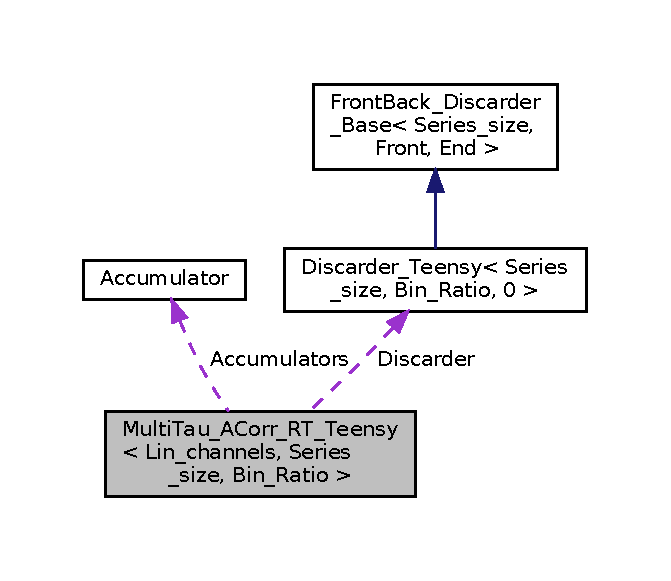
\includegraphics[width=229pt]{classMultiTau__ACorr__RT__Teensy__coll__graph}
\end{center}
\end{figure}
\subsection*{Public Member Functions}
\begin{DoxyCompactItemize}
\item 
\hyperlink{classMultiTau__ACorr__RT__Teensy_a28cfdcd7468aac93693a4d4803fc95f9}{Multi\+Tau\+\_\+\+A\+Corr\+\_\+\+R\+T\+\_\+\+Teensy} ()
\begin{DoxyCompactList}\small\item\em Counts the total number of data points sent to the counter. \end{DoxyCompactList}\item 
void \hyperlink{classMultiTau__ACorr__RT__Teensy_a1ad6126310c987f53a0ec7ab3ae03a12}{push\+\_\+datum} (\hyperlink{types_8hpp_ac89ac912f524b3e3fa3720ea55fec966}{counter\+\_\+t} datum) \hyperlink{utilities_8hpp_a103d5b3998e0dd804213c8f30a094f4d}{\+\_\+\+\_\+attribute\+\_\+\+\_\+}((flatten))
\begin{DoxyCompactList}\small\item\em Pushes the datum to each of the Linear Correlators through the \hyperlink{classAccumulator}{Accumulator} adapter. \end{DoxyCompactList}\item 
void \hyperlink{classMultiTau__ACorr__RT__Teensy_ae36ab4fb6f646d068e638ab7e4ec9da8}{push\+\_\+data} (const \hyperlink{types_8hpp_ac89ac912f524b3e3fa3720ea55fec966}{counter\+\_\+t} $\ast$container, const \hyperlink{types_8hpp_a7c40bb931c31595ed6308605f4537447}{index\+\_\+t} size) \hyperlink{utilities_8hpp_a103d5b3998e0dd804213c8f30a094f4d}{\+\_\+\+\_\+attribute\+\_\+\+\_\+}((flatten))
\begin{DoxyCompactList}\small\item\em Repeatedly calls the Multi\+Tau\+\_\+\+A\+Corr\+\_\+\+R\+T\+::push\+\_\+datum() on the given container of counter values. \end{DoxyCompactList}\item 
void \hyperlink{classMultiTau__ACorr__RT__Teensy_a37a29725971f15305398ac7c9c360eac}{ch\+\_\+out} () const \hyperlink{utilities_8hpp_a103d5b3998e0dd804213c8f30a094f4d}{\+\_\+\+\_\+attribute\+\_\+\+\_\+}((flatten))
\begin{DoxyCompactList}\small\item\em Outputs the Linear Correlator channels through the discarder adapter. \end{DoxyCompactList}\item 
\hyperlink{types_8hpp_a7c40bb931c31595ed6308605f4537447}{index\+\_\+t} \hyperlink{classMultiTau__ACorr__RT__Teensy_a218fdc2fcc3bb7cd5d1c2f03ea2506da}{time\+\_\+scaling\+\_\+factor} () const \hyperlink{utilities_8hpp_a103d5b3998e0dd804213c8f30a094f4d}{\+\_\+\+\_\+attribute\+\_\+\+\_\+}((always\+\_\+inline))
\item 
\hyperlink{types_8hpp_a7c40bb931c31595ed6308605f4537447}{index\+\_\+t} \hyperlink{classMultiTau__ACorr__RT__Teensy_af90bc219b8b9dc316c56efd7c74aae6f}{tau\+\_\+scaling\+\_\+scheme} (unsigned int s) const \hyperlink{utilities_8hpp_a103d5b3998e0dd804213c8f30a094f4d}{\+\_\+\+\_\+attribute\+\_\+\+\_\+}((always\+\_\+inline))
\begin{DoxyCompactList}\small\item\em Returns the relavent Tau scaling factor, based on the specialised scheme. It is used by the accumulator objects to set the Buffer\+Points attribute. \end{DoxyCompactList}\end{DoxyCompactItemize}
\subsection*{Public Attributes}
\begin{DoxyCompactItemize}
\item 
uint32\+\_\+t \hyperlink{classMultiTau__ACorr__RT__Teensy_ac403944f1456e09036bef6dc60d5a0b2}{Data\+Counter} = 0
\begin{DoxyCompactList}\small\item\em Discarder that discards first \#\+Bin\+\_\+\+Ratio points. \end{DoxyCompactList}\end{DoxyCompactItemize}
\subsection*{Private Attributes}
\begin{DoxyCompactItemize}
\item 
\hyperlink{classAccumulator}{Accumulator} \hyperlink{classMultiTau__ACorr__RT__Teensy_a5b6f2659e905f143bc898a9b803eae24}{Accumulators} \mbox{[}Lin\+\_\+channels\mbox{]}
\item 
\hyperlink{classLin__ACorr__RT__Teensy}{Lin\+\_\+\+A\+Corr\+\_\+\+R\+T\+\_\+\+Teensy}$<$ Series\+\_\+size $>$ \hyperlink{classMultiTau__ACorr__RT__Teensy_a1dc1e665268e5774e2810b74e6dbebc4}{Lin\+\_\+\+Corrs} \mbox{[}Lin\+\_\+channels\mbox{]}
\begin{DoxyCompactList}\small\item\em \hyperlink{classAccumulator}{Accumulator} Objects for each channel (\hyperlink{classAccumulator}{Accumulator} \textquotesingle{}0\textquotesingle{} is redundant.) \end{DoxyCompactList}\item 
Serial\+\_\+\+Discarder\+\_\+\+Teensy$<$ Series\+\_\+size, Bin\+\_\+\+Ratio, 0 $>$ \hyperlink{classMultiTau__ACorr__RT__Teensy_ad216281408b0f32892d3c554ad16309e}{Discarder}
\begin{DoxyCompactList}\small\item\em Linear A\+Correlators. \end{DoxyCompactList}\end{DoxyCompactItemize}


\subsection{Detailed Description}
\subsubsection*{template$<$unsigned int Lin\+\_\+channels, index\+\_\+t Series\+\_\+size, unsigned int Bin\+\_\+\+Ratio$>$\newline
class Multi\+Tau\+\_\+\+A\+Corr\+\_\+\+R\+T\+\_\+\+Teensy$<$ Lin\+\_\+channels, Series\+\_\+size, Bin\+\_\+\+Ratio $>$}

Multi\+Tau Auto-\/\+Correlator object that is composed of multiple linear -\/ autocorrelators. Specialised for teensy. 

\subsection{Constructor \& Destructor Documentation}
\mbox{\Hypertarget{classMultiTau__ACorr__RT__Teensy_a28cfdcd7468aac93693a4d4803fc95f9}\label{classMultiTau__ACorr__RT__Teensy_a28cfdcd7468aac93693a4d4803fc95f9}} 
\index{Multi\+Tau\+\_\+\+A\+Corr\+\_\+\+R\+T\+\_\+\+Teensy@{Multi\+Tau\+\_\+\+A\+Corr\+\_\+\+R\+T\+\_\+\+Teensy}!Multi\+Tau\+\_\+\+A\+Corr\+\_\+\+R\+T\+\_\+\+Teensy@{Multi\+Tau\+\_\+\+A\+Corr\+\_\+\+R\+T\+\_\+\+Teensy}}
\index{Multi\+Tau\+\_\+\+A\+Corr\+\_\+\+R\+T\+\_\+\+Teensy@{Multi\+Tau\+\_\+\+A\+Corr\+\_\+\+R\+T\+\_\+\+Teensy}!Multi\+Tau\+\_\+\+A\+Corr\+\_\+\+R\+T\+\_\+\+Teensy@{Multi\+Tau\+\_\+\+A\+Corr\+\_\+\+R\+T\+\_\+\+Teensy}}
\subsubsection{\texorpdfstring{Multi\+Tau\+\_\+\+A\+Corr\+\_\+\+R\+T\+\_\+\+Teensy()}{MultiTau\_ACorr\_RT\_Teensy()}}
{\footnotesize\ttfamily template$<$unsigned int Lin\+\_\+channels, index\+\_\+t Series\+\_\+size, unsigned int Bin\+\_\+\+Ratio$>$ \\
\hyperlink{classMultiTau__ACorr__RT__Teensy}{Multi\+Tau\+\_\+\+A\+Corr\+\_\+\+R\+T\+\_\+\+Teensy}$<$ Lin\+\_\+channels, Series\+\_\+size, Bin\+\_\+\+Ratio $>$\+::\hyperlink{classMultiTau__ACorr__RT__Teensy}{Multi\+Tau\+\_\+\+A\+Corr\+\_\+\+R\+T\+\_\+\+Teensy} (\begin{DoxyParamCaption}{ }\end{DoxyParamCaption})\hspace{0.3cm}{\ttfamily [inline]}}



Counts the total number of data points sent to the counter. 

Default Contructor -\/ Initalizes the Buffer\+Points attribute in the correlators. 

\subsection{Member Function Documentation}
\mbox{\Hypertarget{classMultiTau__ACorr__RT__Teensy_a37a29725971f15305398ac7c9c360eac}\label{classMultiTau__ACorr__RT__Teensy_a37a29725971f15305398ac7c9c360eac}} 
\index{Multi\+Tau\+\_\+\+A\+Corr\+\_\+\+R\+T\+\_\+\+Teensy@{Multi\+Tau\+\_\+\+A\+Corr\+\_\+\+R\+T\+\_\+\+Teensy}!ch\+\_\+out@{ch\+\_\+out}}
\index{ch\+\_\+out@{ch\+\_\+out}!Multi\+Tau\+\_\+\+A\+Corr\+\_\+\+R\+T\+\_\+\+Teensy@{Multi\+Tau\+\_\+\+A\+Corr\+\_\+\+R\+T\+\_\+\+Teensy}}
\subsubsection{\texorpdfstring{ch\+\_\+out()}{ch\_out()}}
{\footnotesize\ttfamily template$<$unsigned int Lin\+\_\+channels, index\+\_\+t Series\+\_\+size, unsigned int Bin\+\_\+\+Ratio$>$ \\
void \hyperlink{classMultiTau__ACorr__RT__Teensy}{Multi\+Tau\+\_\+\+A\+Corr\+\_\+\+R\+T\+\_\+\+Teensy}$<$ Lin\+\_\+channels, Series\+\_\+size, Bin\+\_\+\+Ratio $>$\+::ch\+\_\+out (\begin{DoxyParamCaption}{ }\end{DoxyParamCaption}) const\hspace{0.3cm}{\ttfamily [inline]}}



Outputs the Linear Correlator channels through the discarder adapter. 

\mbox{\Hypertarget{classMultiTau__ACorr__RT__Teensy_ae36ab4fb6f646d068e638ab7e4ec9da8}\label{classMultiTau__ACorr__RT__Teensy_ae36ab4fb6f646d068e638ab7e4ec9da8}} 
\index{Multi\+Tau\+\_\+\+A\+Corr\+\_\+\+R\+T\+\_\+\+Teensy@{Multi\+Tau\+\_\+\+A\+Corr\+\_\+\+R\+T\+\_\+\+Teensy}!push\+\_\+data@{push\+\_\+data}}
\index{push\+\_\+data@{push\+\_\+data}!Multi\+Tau\+\_\+\+A\+Corr\+\_\+\+R\+T\+\_\+\+Teensy@{Multi\+Tau\+\_\+\+A\+Corr\+\_\+\+R\+T\+\_\+\+Teensy}}
\subsubsection{\texorpdfstring{push\+\_\+data()}{push\_data()}}
{\footnotesize\ttfamily template$<$unsigned int Lin\+\_\+channels, index\+\_\+t Series\+\_\+size, unsigned int Bin\+\_\+\+Ratio$>$ \\
void \hyperlink{classMultiTau__ACorr__RT__Teensy}{Multi\+Tau\+\_\+\+A\+Corr\+\_\+\+R\+T\+\_\+\+Teensy}$<$ Lin\+\_\+channels, Series\+\_\+size, Bin\+\_\+\+Ratio $>$\+::push\+\_\+data (\begin{DoxyParamCaption}\item[{const \hyperlink{types_8hpp_ac89ac912f524b3e3fa3720ea55fec966}{counter\+\_\+t} $\ast$}]{container,  }\item[{const \hyperlink{types_8hpp_a7c40bb931c31595ed6308605f4537447}{index\+\_\+t}}]{size }\end{DoxyParamCaption})\hspace{0.3cm}{\ttfamily [inline]}}



Repeatedly calls the Multi\+Tau\+\_\+\+A\+Corr\+\_\+\+R\+T\+::push\+\_\+datum() on the given container of counter values. 

\mbox{\Hypertarget{classMultiTau__ACorr__RT__Teensy_a1ad6126310c987f53a0ec7ab3ae03a12}\label{classMultiTau__ACorr__RT__Teensy_a1ad6126310c987f53a0ec7ab3ae03a12}} 
\index{Multi\+Tau\+\_\+\+A\+Corr\+\_\+\+R\+T\+\_\+\+Teensy@{Multi\+Tau\+\_\+\+A\+Corr\+\_\+\+R\+T\+\_\+\+Teensy}!push\+\_\+datum@{push\+\_\+datum}}
\index{push\+\_\+datum@{push\+\_\+datum}!Multi\+Tau\+\_\+\+A\+Corr\+\_\+\+R\+T\+\_\+\+Teensy@{Multi\+Tau\+\_\+\+A\+Corr\+\_\+\+R\+T\+\_\+\+Teensy}}
\subsubsection{\texorpdfstring{push\+\_\+datum()}{push\_datum()}}
{\footnotesize\ttfamily template$<$unsigned int Lin\+\_\+channels, index\+\_\+t Series\+\_\+size, unsigned int Bin\+\_\+\+Ratio$>$ \\
void \hyperlink{classMultiTau__ACorr__RT__Teensy}{Multi\+Tau\+\_\+\+A\+Corr\+\_\+\+R\+T\+\_\+\+Teensy}$<$ Lin\+\_\+channels, Series\+\_\+size, Bin\+\_\+\+Ratio $>$\+::push\+\_\+datum (\begin{DoxyParamCaption}\item[{\hyperlink{types_8hpp_ac89ac912f524b3e3fa3720ea55fec966}{counter\+\_\+t}}]{datum }\end{DoxyParamCaption})\hspace{0.3cm}{\ttfamily [inline]}}



Pushes the datum to each of the Linear Correlators through the \hyperlink{classAccumulator}{Accumulator} adapter. 

\mbox{\Hypertarget{classMultiTau__ACorr__RT__Teensy_af90bc219b8b9dc316c56efd7c74aae6f}\label{classMultiTau__ACorr__RT__Teensy_af90bc219b8b9dc316c56efd7c74aae6f}} 
\index{Multi\+Tau\+\_\+\+A\+Corr\+\_\+\+R\+T\+\_\+\+Teensy@{Multi\+Tau\+\_\+\+A\+Corr\+\_\+\+R\+T\+\_\+\+Teensy}!tau\+\_\+scaling\+\_\+scheme@{tau\+\_\+scaling\+\_\+scheme}}
\index{tau\+\_\+scaling\+\_\+scheme@{tau\+\_\+scaling\+\_\+scheme}!Multi\+Tau\+\_\+\+A\+Corr\+\_\+\+R\+T\+\_\+\+Teensy@{Multi\+Tau\+\_\+\+A\+Corr\+\_\+\+R\+T\+\_\+\+Teensy}}
\subsubsection{\texorpdfstring{tau\+\_\+scaling\+\_\+scheme()}{tau\_scaling\_scheme()}}
{\footnotesize\ttfamily template$<$unsigned int Lin\+\_\+channels, index\+\_\+t Series\+\_\+size, unsigned int Bin\+\_\+\+Ratio$>$ \\
\hyperlink{types_8hpp_a7c40bb931c31595ed6308605f4537447}{index\+\_\+t} \hyperlink{classMultiTau__ACorr__RT__Teensy}{Multi\+Tau\+\_\+\+A\+Corr\+\_\+\+R\+T\+\_\+\+Teensy}$<$ Lin\+\_\+channels, Series\+\_\+size, Bin\+\_\+\+Ratio $>$\+::tau\+\_\+scaling\+\_\+scheme (\begin{DoxyParamCaption}\item[{unsigned int}]{s }\end{DoxyParamCaption}) const\hspace{0.3cm}{\ttfamily [inline]}}



Returns the relavent Tau scaling factor, based on the specialised scheme. It is used by the accumulator objects to set the Buffer\+Points attribute. 

\mbox{\Hypertarget{classMultiTau__ACorr__RT__Teensy_a218fdc2fcc3bb7cd5d1c2f03ea2506da}\label{classMultiTau__ACorr__RT__Teensy_a218fdc2fcc3bb7cd5d1c2f03ea2506da}} 
\index{Multi\+Tau\+\_\+\+A\+Corr\+\_\+\+R\+T\+\_\+\+Teensy@{Multi\+Tau\+\_\+\+A\+Corr\+\_\+\+R\+T\+\_\+\+Teensy}!time\+\_\+scaling\+\_\+factor@{time\+\_\+scaling\+\_\+factor}}
\index{time\+\_\+scaling\+\_\+factor@{time\+\_\+scaling\+\_\+factor}!Multi\+Tau\+\_\+\+A\+Corr\+\_\+\+R\+T\+\_\+\+Teensy@{Multi\+Tau\+\_\+\+A\+Corr\+\_\+\+R\+T\+\_\+\+Teensy}}
\subsubsection{\texorpdfstring{time\+\_\+scaling\+\_\+factor()}{time\_scaling\_factor()}}
{\footnotesize\ttfamily template$<$unsigned int Lin\+\_\+channels, index\+\_\+t Series\+\_\+size, unsigned int Bin\+\_\+\+Ratio$>$ \\
\hyperlink{types_8hpp_a7c40bb931c31595ed6308605f4537447}{index\+\_\+t} \hyperlink{classMultiTau__ACorr__RT__Teensy}{Multi\+Tau\+\_\+\+A\+Corr\+\_\+\+R\+T\+\_\+\+Teensy}$<$ Lin\+\_\+channels, Series\+\_\+size, Bin\+\_\+\+Ratio $>$\+::time\+\_\+scaling\+\_\+factor (\begin{DoxyParamCaption}{ }\end{DoxyParamCaption}) const\hspace{0.3cm}{\ttfamily [inline]}}

Returns the number of data points after which, the timescale is scaled according to the Multi\+Tau\+\_\+\+A\+Corr\+\_\+\+R\+T\+::tau\+\_\+scaling\+\_\+scheme(). 

\subsection{Member Data Documentation}
\mbox{\Hypertarget{classMultiTau__ACorr__RT__Teensy_a5b6f2659e905f143bc898a9b803eae24}\label{classMultiTau__ACorr__RT__Teensy_a5b6f2659e905f143bc898a9b803eae24}} 
\index{Multi\+Tau\+\_\+\+A\+Corr\+\_\+\+R\+T\+\_\+\+Teensy@{Multi\+Tau\+\_\+\+A\+Corr\+\_\+\+R\+T\+\_\+\+Teensy}!Accumulators@{Accumulators}}
\index{Accumulators@{Accumulators}!Multi\+Tau\+\_\+\+A\+Corr\+\_\+\+R\+T\+\_\+\+Teensy@{Multi\+Tau\+\_\+\+A\+Corr\+\_\+\+R\+T\+\_\+\+Teensy}}
\subsubsection{\texorpdfstring{Accumulators}{Accumulators}}
{\footnotesize\ttfamily template$<$unsigned int Lin\+\_\+channels, index\+\_\+t Series\+\_\+size, unsigned int Bin\+\_\+\+Ratio$>$ \\
\hyperlink{classAccumulator}{Accumulator} \hyperlink{classMultiTau__ACorr__RT__Teensy}{Multi\+Tau\+\_\+\+A\+Corr\+\_\+\+R\+T\+\_\+\+Teensy}$<$ Lin\+\_\+channels, Series\+\_\+size, Bin\+\_\+\+Ratio $>$\+::Accumulators\mbox{[}Lin\+\_\+channels\mbox{]}\hspace{0.3cm}{\ttfamily [private]}}

\mbox{\Hypertarget{classMultiTau__ACorr__RT__Teensy_ac403944f1456e09036bef6dc60d5a0b2}\label{classMultiTau__ACorr__RT__Teensy_ac403944f1456e09036bef6dc60d5a0b2}} 
\index{Multi\+Tau\+\_\+\+A\+Corr\+\_\+\+R\+T\+\_\+\+Teensy@{Multi\+Tau\+\_\+\+A\+Corr\+\_\+\+R\+T\+\_\+\+Teensy}!Data\+Counter@{Data\+Counter}}
\index{Data\+Counter@{Data\+Counter}!Multi\+Tau\+\_\+\+A\+Corr\+\_\+\+R\+T\+\_\+\+Teensy@{Multi\+Tau\+\_\+\+A\+Corr\+\_\+\+R\+T\+\_\+\+Teensy}}
\subsubsection{\texorpdfstring{Data\+Counter}{DataCounter}}
{\footnotesize\ttfamily template$<$unsigned int Lin\+\_\+channels, index\+\_\+t Series\+\_\+size, unsigned int Bin\+\_\+\+Ratio$>$ \\
uint32\+\_\+t \hyperlink{classMultiTau__ACorr__RT__Teensy}{Multi\+Tau\+\_\+\+A\+Corr\+\_\+\+R\+T\+\_\+\+Teensy}$<$ Lin\+\_\+channels, Series\+\_\+size, Bin\+\_\+\+Ratio $>$\+::Data\+Counter = 0}



Discarder that discards first \#\+Bin\+\_\+\+Ratio points. 

\mbox{\Hypertarget{classMultiTau__ACorr__RT__Teensy_ad216281408b0f32892d3c554ad16309e}\label{classMultiTau__ACorr__RT__Teensy_ad216281408b0f32892d3c554ad16309e}} 
\index{Multi\+Tau\+\_\+\+A\+Corr\+\_\+\+R\+T\+\_\+\+Teensy@{Multi\+Tau\+\_\+\+A\+Corr\+\_\+\+R\+T\+\_\+\+Teensy}!Discarder@{Discarder}}
\index{Discarder@{Discarder}!Multi\+Tau\+\_\+\+A\+Corr\+\_\+\+R\+T\+\_\+\+Teensy@{Multi\+Tau\+\_\+\+A\+Corr\+\_\+\+R\+T\+\_\+\+Teensy}}
\subsubsection{\texorpdfstring{Discarder}{Discarder}}
{\footnotesize\ttfamily template$<$unsigned int Lin\+\_\+channels, index\+\_\+t Series\+\_\+size, unsigned int Bin\+\_\+\+Ratio$>$ \\
Serial\+\_\+\+Discarder\+\_\+\+Teensy$<$Series\+\_\+size, Bin\+\_\+\+Ratio, 0$>$ \hyperlink{classMultiTau__ACorr__RT__Teensy}{Multi\+Tau\+\_\+\+A\+Corr\+\_\+\+R\+T\+\_\+\+Teensy}$<$ Lin\+\_\+channels, Series\+\_\+size, Bin\+\_\+\+Ratio $>$\+::Discarder\hspace{0.3cm}{\ttfamily [private]}}



Linear A\+Correlators. 

\mbox{\Hypertarget{classMultiTau__ACorr__RT__Teensy_a1dc1e665268e5774e2810b74e6dbebc4}\label{classMultiTau__ACorr__RT__Teensy_a1dc1e665268e5774e2810b74e6dbebc4}} 
\index{Multi\+Tau\+\_\+\+A\+Corr\+\_\+\+R\+T\+\_\+\+Teensy@{Multi\+Tau\+\_\+\+A\+Corr\+\_\+\+R\+T\+\_\+\+Teensy}!Lin\+\_\+\+Corrs@{Lin\+\_\+\+Corrs}}
\index{Lin\+\_\+\+Corrs@{Lin\+\_\+\+Corrs}!Multi\+Tau\+\_\+\+A\+Corr\+\_\+\+R\+T\+\_\+\+Teensy@{Multi\+Tau\+\_\+\+A\+Corr\+\_\+\+R\+T\+\_\+\+Teensy}}
\subsubsection{\texorpdfstring{Lin\+\_\+\+Corrs}{Lin\_Corrs}}
{\footnotesize\ttfamily template$<$unsigned int Lin\+\_\+channels, index\+\_\+t Series\+\_\+size, unsigned int Bin\+\_\+\+Ratio$>$ \\
\hyperlink{classLin__ACorr__RT__Teensy}{Lin\+\_\+\+A\+Corr\+\_\+\+R\+T\+\_\+\+Teensy}$<$Series\+\_\+size$>$ \hyperlink{classMultiTau__ACorr__RT__Teensy}{Multi\+Tau\+\_\+\+A\+Corr\+\_\+\+R\+T\+\_\+\+Teensy}$<$ Lin\+\_\+channels, Series\+\_\+size, Bin\+\_\+\+Ratio $>$\+::Lin\+\_\+\+Corrs\mbox{[}Lin\+\_\+channels\mbox{]}\hspace{0.3cm}{\ttfamily [private]}}



\hyperlink{classAccumulator}{Accumulator} Objects for each channel (\hyperlink{classAccumulator}{Accumulator} \textquotesingle{}0\textquotesingle{} is redundant.) 



The documentation for this class was generated from the following file\+:\begin{DoxyCompactItemize}
\item 
/mnt/m/code/\+Correlator/\+Software/\hyperlink{multi__tau_8hpp}{multi\+\_\+tau.\+hpp}\end{DoxyCompactItemize}

\hypertarget{classPIT__LifetimeTimer}{}\section{P\+I\+T\+\_\+\+Lifetime\+Timer Class Reference}
\label{classPIT__LifetimeTimer}\index{P\+I\+T\+\_\+\+Lifetime\+Timer@{P\+I\+T\+\_\+\+Lifetime\+Timer}}


Interface for using the \char`\"{}\+Life Time T\+Imer\char`\"{} functionality of the Periodic Interrut Timer on Teensy 4.\+x microcontrollers. The module uses Channel 0 and 1 of the 4 P\+IT channels.  




{\ttfamily \#include $<$lifetime\+\_\+timer.\+hpp$>$}

\subsection*{Public Member Functions}
\begin{DoxyCompactItemize}
\item 
\hyperlink{classPIT__LifetimeTimer_a826797e75688ab4e7cd5c8854fa6a7c0}{P\+I\+T\+\_\+\+Lifetime\+Timer} ()
\item 
void \hyperlink{classPIT__LifetimeTimer_ad1c585d138123be94769afcca87f2dc6}{init} () \+\_\+\+\_\+attribute\+\_\+\+\_\+((always\+\_\+inline))
\begin{DoxyCompactList}\small\item\em Sets up Timer 0 and Timer 1 channels for Lifetime timing -\/ chained configuration. This function also makes a call to enable P\+IT timers. The timers are aet at maximum values and will start downcounting once \hyperlink{classPIT__LifetimeTimer_a6feabeff2529cabaf27ef53d027a4fc9}{P\+I\+T\+\_\+\+Lifetime\+Timer\+::start()} method is called. \end{DoxyCompactList}\item 
void \hyperlink{classPIT__LifetimeTimer_a6feabeff2529cabaf27ef53d027a4fc9}{start} () \+\_\+\+\_\+attribute\+\_\+\+\_\+((always\+\_\+inline))
\begin{DoxyCompactList}\small\item\em Starts the timers for down counting. \end{DoxyCompactList}\item 
void \hyperlink{classPIT__LifetimeTimer_a92543f292044725b1dea4d009e01d9e4}{stop} () \+\_\+\+\_\+attribute\+\_\+\+\_\+((always\+\_\+inline))
\begin{DoxyCompactList}\small\item\em Stops the timers from counting. The timers values will freeze. \end{DoxyCompactList}\item 
void \hyperlink{classPIT__LifetimeTimer_a5c1c38cfa6c7a049a495ee3d89e13276}{reset} () \+\_\+\+\_\+attribute\+\_\+\+\_\+((always\+\_\+inline))
\begin{DoxyCompactList}\small\item\em Stops the timers and resets the timer back to the init value (max) -\/ 0x\+F\+F\+F\+F\+F\+F\+F\+F\+F\+F\+F\+F\+FF. \end{DoxyCompactList}\item 
uint64\+\_\+t \hyperlink{classPIT__LifetimeTimer_a4ee08cce7812322a7a10fcba0463476c}{read\+\_\+val} () \+\_\+\+\_\+attribute\+\_\+\+\_\+((always\+\_\+inline))
\begin{DoxyCompactList}\small\item\em Returns the complete 64-\/bit timing value. \end{DoxyCompactList}\item 
uint32\+\_\+t \hyperlink{classPIT__LifetimeTimer_a4f7f8cd3847b9edb19dfa27f048a08cc}{read\+\_\+low\+\_\+val} () \+\_\+\+\_\+attribute\+\_\+\+\_\+((always\+\_\+inline))
\begin{DoxyCompactList}\small\item\em Returns the lower 32-\/bit half of the 64-\/bit timing value. \end{DoxyCompactList}\item 
uint32\+\_\+t \hyperlink{classPIT__LifetimeTimer_a39b0861ac88aec5e53f326409d536bcf}{read\+\_\+high\+\_\+val} () \+\_\+\+\_\+attribute\+\_\+\+\_\+((always\+\_\+inline))
\begin{DoxyCompactList}\small\item\em Returns the higher 32-\/bit half of the 64-\/bit timing value. \end{DoxyCompactList}\item 
uint64\+\_\+t \hyperlink{classPIT__LifetimeTimer_a04adf2272a47d4c81a28c6363e2da4fd}{elapsed64} () \+\_\+\+\_\+attribute\+\_\+\+\_\+((always\+\_\+inline))
\begin{DoxyCompactList}\small\item\em Returns the elapsed duration from the start call of the timer. The return is the complete 64bit value. \end{DoxyCompactList}\item 
uint32\+\_\+t \hyperlink{classPIT__LifetimeTimer_af7481214070333f845a23456b4d75880}{elapsed32} () \+\_\+\+\_\+attribute\+\_\+\+\_\+((always\+\_\+inline))
\begin{DoxyCompactList}\small\item\em Returns the elapsed duration from the start call of the timer. The return is the lower 32-\/bit half elapsed time value. \end{DoxyCompactList}\end{DoxyCompactItemize}


\subsection{Detailed Description}
Interface for using the \char`\"{}\+Life Time T\+Imer\char`\"{} functionality of the Periodic Interrut Timer on Teensy 4.\+x microcontrollers. The module uses Channel 0 and 1 of the 4 P\+IT channels. 

\begin{DoxyAttention}{Attention}
The module has no checks on the use of C\+H0 and C\+H1 by external drivers, however, the interface enforces a singleton template and can only be constructed once. 

The module does not set the clock frequency and uses either the default or the one set globally (as is the only use case) by external drivers outside its scope. 

Source \+: Code adapted from I\+M\+X\+RT Manual Page 2977. 
\end{DoxyAttention}
\begin{DoxyRefDesc}{Todo}
\item[\hyperlink{todo__todo000002}{Todo}]Resolve Singleton template -\/ constexpr static issue. \end{DoxyRefDesc}


\subsection{Constructor \& Destructor Documentation}
\mbox{\Hypertarget{classPIT__LifetimeTimer_a826797e75688ab4e7cd5c8854fa6a7c0}\label{classPIT__LifetimeTimer_a826797e75688ab4e7cd5c8854fa6a7c0}} 
\index{P\+I\+T\+\_\+\+Lifetime\+Timer@{P\+I\+T\+\_\+\+Lifetime\+Timer}!P\+I\+T\+\_\+\+Lifetime\+Timer@{P\+I\+T\+\_\+\+Lifetime\+Timer}}
\index{P\+I\+T\+\_\+\+Lifetime\+Timer@{P\+I\+T\+\_\+\+Lifetime\+Timer}!P\+I\+T\+\_\+\+Lifetime\+Timer@{P\+I\+T\+\_\+\+Lifetime\+Timer}}
\subsubsection{\texorpdfstring{P\+I\+T\+\_\+\+Lifetime\+Timer()}{PIT\_LifetimeTimer()}}
{\footnotesize\ttfamily P\+I\+T\+\_\+\+Lifetime\+Timer\+::\+P\+I\+T\+\_\+\+Lifetime\+Timer (\begin{DoxyParamCaption}{ }\end{DoxyParamCaption})\hspace{0.3cm}{\ttfamily [inline]}}



\subsection{Member Function Documentation}
\mbox{\Hypertarget{classPIT__LifetimeTimer_af7481214070333f845a23456b4d75880}\label{classPIT__LifetimeTimer_af7481214070333f845a23456b4d75880}} 
\index{P\+I\+T\+\_\+\+Lifetime\+Timer@{P\+I\+T\+\_\+\+Lifetime\+Timer}!elapsed32@{elapsed32}}
\index{elapsed32@{elapsed32}!P\+I\+T\+\_\+\+Lifetime\+Timer@{P\+I\+T\+\_\+\+Lifetime\+Timer}}
\subsubsection{\texorpdfstring{elapsed32()}{elapsed32()}}
{\footnotesize\ttfamily uint32\+\_\+t P\+I\+T\+\_\+\+Lifetime\+Timer\+::elapsed32 (\begin{DoxyParamCaption}{ }\end{DoxyParamCaption})\hspace{0.3cm}{\ttfamily [inline]}}



Returns the elapsed duration from the start call of the timer. The return is the lower 32-\/bit half elapsed time value. 

\begin{DoxyWarning}{Warning}
If the elapsed duration is greater than the 32-\/bit rollover time, then the quantity returned is meaningless. Hence, use of this function should be reserved for measuring small time durarions. 
\end{DoxyWarning}
\mbox{\Hypertarget{classPIT__LifetimeTimer_a04adf2272a47d4c81a28c6363e2da4fd}\label{classPIT__LifetimeTimer_a04adf2272a47d4c81a28c6363e2da4fd}} 
\index{P\+I\+T\+\_\+\+Lifetime\+Timer@{P\+I\+T\+\_\+\+Lifetime\+Timer}!elapsed64@{elapsed64}}
\index{elapsed64@{elapsed64}!P\+I\+T\+\_\+\+Lifetime\+Timer@{P\+I\+T\+\_\+\+Lifetime\+Timer}}
\subsubsection{\texorpdfstring{elapsed64()}{elapsed64()}}
{\footnotesize\ttfamily uint64\+\_\+t P\+I\+T\+\_\+\+Lifetime\+Timer\+::elapsed64 (\begin{DoxyParamCaption}{ }\end{DoxyParamCaption})\hspace{0.3cm}{\ttfamily [inline]}}



Returns the elapsed duration from the start call of the timer. The return is the complete 64bit value. 

\mbox{\Hypertarget{classPIT__LifetimeTimer_ad1c585d138123be94769afcca87f2dc6}\label{classPIT__LifetimeTimer_ad1c585d138123be94769afcca87f2dc6}} 
\index{P\+I\+T\+\_\+\+Lifetime\+Timer@{P\+I\+T\+\_\+\+Lifetime\+Timer}!init@{init}}
\index{init@{init}!P\+I\+T\+\_\+\+Lifetime\+Timer@{P\+I\+T\+\_\+\+Lifetime\+Timer}}
\subsubsection{\texorpdfstring{init()}{init()}}
{\footnotesize\ttfamily void P\+I\+T\+\_\+\+Lifetime\+Timer\+::init (\begin{DoxyParamCaption}{ }\end{DoxyParamCaption})\hspace{0.3cm}{\ttfamily [inline]}}



Sets up Timer 0 and Timer 1 channels for Lifetime timing -\/ chained configuration. This function also makes a call to enable P\+IT timers. The timers are aet at maximum values and will start downcounting once \hyperlink{classPIT__LifetimeTimer_a6feabeff2529cabaf27ef53d027a4fc9}{P\+I\+T\+\_\+\+Lifetime\+Timer\+::start()} method is called. 

\begin{DoxyAttention}{Attention}
Reference \+: Code adapted from I\+M\+X\+RT Manual Page 2977. 

The timers will operate at the clock frequency set for P\+IT timers outside this library. 
\end{DoxyAttention}
\mbox{\Hypertarget{classPIT__LifetimeTimer_a39b0861ac88aec5e53f326409d536bcf}\label{classPIT__LifetimeTimer_a39b0861ac88aec5e53f326409d536bcf}} 
\index{P\+I\+T\+\_\+\+Lifetime\+Timer@{P\+I\+T\+\_\+\+Lifetime\+Timer}!read\+\_\+high\+\_\+val@{read\+\_\+high\+\_\+val}}
\index{read\+\_\+high\+\_\+val@{read\+\_\+high\+\_\+val}!P\+I\+T\+\_\+\+Lifetime\+Timer@{P\+I\+T\+\_\+\+Lifetime\+Timer}}
\subsubsection{\texorpdfstring{read\+\_\+high\+\_\+val()}{read\_high\_val()}}
{\footnotesize\ttfamily uint32\+\_\+t P\+I\+T\+\_\+\+Lifetime\+Timer\+::read\+\_\+high\+\_\+val (\begin{DoxyParamCaption}{ }\end{DoxyParamCaption})\hspace{0.3cm}{\ttfamily [inline]}}



Returns the higher 32-\/bit half of the 64-\/bit timing value. 

\mbox{\Hypertarget{classPIT__LifetimeTimer_a4f7f8cd3847b9edb19dfa27f048a08cc}\label{classPIT__LifetimeTimer_a4f7f8cd3847b9edb19dfa27f048a08cc}} 
\index{P\+I\+T\+\_\+\+Lifetime\+Timer@{P\+I\+T\+\_\+\+Lifetime\+Timer}!read\+\_\+low\+\_\+val@{read\+\_\+low\+\_\+val}}
\index{read\+\_\+low\+\_\+val@{read\+\_\+low\+\_\+val}!P\+I\+T\+\_\+\+Lifetime\+Timer@{P\+I\+T\+\_\+\+Lifetime\+Timer}}
\subsubsection{\texorpdfstring{read\+\_\+low\+\_\+val()}{read\_low\_val()}}
{\footnotesize\ttfamily uint32\+\_\+t P\+I\+T\+\_\+\+Lifetime\+Timer\+::read\+\_\+low\+\_\+val (\begin{DoxyParamCaption}{ }\end{DoxyParamCaption})\hspace{0.3cm}{\ttfamily [inline]}}



Returns the lower 32-\/bit half of the 64-\/bit timing value. 

\mbox{\Hypertarget{classPIT__LifetimeTimer_a4ee08cce7812322a7a10fcba0463476c}\label{classPIT__LifetimeTimer_a4ee08cce7812322a7a10fcba0463476c}} 
\index{P\+I\+T\+\_\+\+Lifetime\+Timer@{P\+I\+T\+\_\+\+Lifetime\+Timer}!read\+\_\+val@{read\+\_\+val}}
\index{read\+\_\+val@{read\+\_\+val}!P\+I\+T\+\_\+\+Lifetime\+Timer@{P\+I\+T\+\_\+\+Lifetime\+Timer}}
\subsubsection{\texorpdfstring{read\+\_\+val()}{read\_val()}}
{\footnotesize\ttfamily uint64\+\_\+t P\+I\+T\+\_\+\+Lifetime\+Timer\+::read\+\_\+val (\begin{DoxyParamCaption}{ }\end{DoxyParamCaption})\hspace{0.3cm}{\ttfamily [inline]}}



Returns the complete 64-\/bit timing value. 

\mbox{\Hypertarget{classPIT__LifetimeTimer_a5c1c38cfa6c7a049a495ee3d89e13276}\label{classPIT__LifetimeTimer_a5c1c38cfa6c7a049a495ee3d89e13276}} 
\index{P\+I\+T\+\_\+\+Lifetime\+Timer@{P\+I\+T\+\_\+\+Lifetime\+Timer}!reset@{reset}}
\index{reset@{reset}!P\+I\+T\+\_\+\+Lifetime\+Timer@{P\+I\+T\+\_\+\+Lifetime\+Timer}}
\subsubsection{\texorpdfstring{reset()}{reset()}}
{\footnotesize\ttfamily void P\+I\+T\+\_\+\+Lifetime\+Timer\+::reset (\begin{DoxyParamCaption}{ }\end{DoxyParamCaption})\hspace{0.3cm}{\ttfamily [inline]}}



Stops the timers and resets the timer back to the init value (max) -\/ 0x\+F\+F\+F\+F\+F\+F\+F\+F\+F\+F\+F\+F\+FF. 

\mbox{\Hypertarget{classPIT__LifetimeTimer_a6feabeff2529cabaf27ef53d027a4fc9}\label{classPIT__LifetimeTimer_a6feabeff2529cabaf27ef53d027a4fc9}} 
\index{P\+I\+T\+\_\+\+Lifetime\+Timer@{P\+I\+T\+\_\+\+Lifetime\+Timer}!start@{start}}
\index{start@{start}!P\+I\+T\+\_\+\+Lifetime\+Timer@{P\+I\+T\+\_\+\+Lifetime\+Timer}}
\subsubsection{\texorpdfstring{start()}{start()}}
{\footnotesize\ttfamily void P\+I\+T\+\_\+\+Lifetime\+Timer\+::start (\begin{DoxyParamCaption}{ }\end{DoxyParamCaption})\hspace{0.3cm}{\ttfamily [inline]}}



Starts the timers for down counting. 

\mbox{\Hypertarget{classPIT__LifetimeTimer_a92543f292044725b1dea4d009e01d9e4}\label{classPIT__LifetimeTimer_a92543f292044725b1dea4d009e01d9e4}} 
\index{P\+I\+T\+\_\+\+Lifetime\+Timer@{P\+I\+T\+\_\+\+Lifetime\+Timer}!stop@{stop}}
\index{stop@{stop}!P\+I\+T\+\_\+\+Lifetime\+Timer@{P\+I\+T\+\_\+\+Lifetime\+Timer}}
\subsubsection{\texorpdfstring{stop()}{stop()}}
{\footnotesize\ttfamily void P\+I\+T\+\_\+\+Lifetime\+Timer\+::stop (\begin{DoxyParamCaption}{ }\end{DoxyParamCaption})\hspace{0.3cm}{\ttfamily [inline]}}



Stops the timers from counting. The timers values will freeze. 



The documentation for this class was generated from the following file\+:\begin{DoxyCompactItemize}
\item 
code/hardware/\hyperlink{lifetime__timer_8hpp}{lifetime\+\_\+timer.\+hpp}\end{DoxyCompactItemize}

\hypertarget{classPITController}{}\section{P\+I\+T\+Controller$<$ Ch\+ID $>$ Class Template Reference}
\label{classPITController}\index{P\+I\+T\+Controller$<$ Ch\+I\+D $>$@{P\+I\+T\+Controller$<$ Ch\+I\+D $>$}}


Interface for P\+IT timers on Teensy 4.\+x microcontrollers.  




{\ttfamily \#include $<$pit.\+hpp$>$}

\subsection*{Public Member Functions}
\begin{DoxyCompactItemize}
\item 
\hyperlink{classPITController_ad9ef4f151495076fad7b0c556e48b117}{P\+I\+T\+Controller} ()
\begin{DoxyCompactList}\small\item\em Constant -\/ Maximum possible counter value. 32 bit counter. \end{DoxyCompactList}\item 
void \hyperlink{group__Controls_ga4dae1ed0ada64ebc03665e8f39795e7e}{start} () \hyperlink{utilities_8hpp_a103d5b3998e0dd804213c8f30a094f4d}{\+\_\+\+\_\+attribute\+\_\+\+\_\+}((always\+\_\+inline))
\begin{DoxyCompactList}\small\item\em Start counting on the timer. \end{DoxyCompactList}\item 
void \hyperlink{group__Controls_ga5a6e2b00c6355934531a77a62660bec7}{stop} () \hyperlink{utilities_8hpp_a103d5b3998e0dd804213c8f30a094f4d}{\+\_\+\+\_\+attribute\+\_\+\+\_\+}((always\+\_\+inline))
\begin{DoxyCompactList}\small\item\em stop counting on the timer. \end{DoxyCompactList}\item 
\hyperlink{errors_8hpp_a4e8c0d09726859e3d3369c0da5a1aa7f}{Error\+\_\+t} \hyperlink{group__Controls_gaaf7a79129a4ea5af057ea8f537b7ae9f}{set\+\_\+gate\+\_\+time} (double gt\+\_\+microseconds) \hyperlink{utilities_8hpp_a103d5b3998e0dd804213c8f30a094f4d}{\+\_\+\+\_\+attribute\+\_\+\+\_\+}((flatten))
\begin{DoxyCompactList}\small\item\em Sets the gate time after which the counter returns to zero and marks the end of onegate interval. \end{DoxyCompactList}\item 
double \hyperlink{group__Controls_ga3fedb5ff5a44b664e8132f4e2836b155}{period\+\_\+error\+\_\+us} () const \hyperlink{utilities_8hpp_a103d5b3998e0dd804213c8f30a094f4d}{\+\_\+\+\_\+attribute\+\_\+\+\_\+}((always\+\_\+inline))
\begin{DoxyCompactList}\small\item\em Returns the error in the gate timing period due to the finite resolution of the timers.  Error in microseconds. \end{DoxyCompactList}\item 
double \hyperlink{group__Controls_ga2b64ce8a01dc1254002c4ff3c384a6fd}{tick\+\_\+period\+\_\+us} () \hyperlink{utilities_8hpp_a103d5b3998e0dd804213c8f30a094f4d}{\+\_\+\+\_\+attribute\+\_\+\+\_\+}((always\+\_\+inline))
\begin{DoxyCompactList}\small\item\em Returns the value of one {\bfseries Tick} -\/ Minimum resolution of the timer. \end{DoxyCompactList}\item 
void \hyperlink{group__Controls_ga19f11a8cdb94353ffaaa5a2eccf35ee5}{get\+\_\+xbar\+\_\+in\+\_\+pin} () \hyperlink{utilities_8hpp_a103d5b3998e0dd804213c8f30a094f4d}{\+\_\+\+\_\+attribute\+\_\+\+\_\+}((always\+\_\+inline))
\begin{DoxyCompactList}\small\item\em Returns the correspoding X\+B\+A\+R1-\/A Input Pins for the corresponding channel T\+R\+I\+G\+G\+ER signal.  -\/ Manual Page 63. \end{DoxyCompactList}\item 
void \hyperlink{group__Interrupt_gaf1a21e0b3f9a57e247aa40c457e15ee3}{interrupt} () \hyperlink{utilities_8hpp_a103d5b3998e0dd804213c8f30a094f4d}{\+\_\+\+\_\+attribute\+\_\+\+\_\+}((always\+\_\+inline))
\begin{DoxyCompactList}\small\item\em Enable Interruptsthat are triggered after one gate time completion. \end{DoxyCompactList}\item 
void \hyperlink{group__Interrupt_ga6e36c84f319e52e5a14ca20f299b64b5}{no\+\_\+interrupt} () \hyperlink{utilities_8hpp_a103d5b3998e0dd804213c8f30a094f4d}{\+\_\+\+\_\+attribute\+\_\+\+\_\+}((always\+\_\+inline))
\begin{DoxyCompactList}\small\item\em Disable Interrupts that are triggered after one gate time completion. \end{DoxyCompactList}\item 
void \hyperlink{group__Interrupt_gae3f9c981e88cced34153234475de5646}{clear\+\_\+interrupt\+\_\+flag} () \hyperlink{utilities_8hpp_a103d5b3998e0dd804213c8f30a094f4d}{\+\_\+\+\_\+attribute\+\_\+\+\_\+}((always\+\_\+inline))
\begin{DoxyCompactList}\small\item\em Clears the interrupt flag and hence prepares the timer for the next gate interval. The clearing has to be done manually. If the flag is not cleared, the interrupt will be called again and again. \end{DoxyCompactList}\item 
void \hyperlink{group__CLK_ga63e67e2ebfd6ceb5f5e38d9bd6a54754}{sel\+\_\+\+F\+B\+U\+S\+\_\+clock} () \hyperlink{utilities_8hpp_a103d5b3998e0dd804213c8f30a094f4d}{\+\_\+\+\_\+attribute\+\_\+\+\_\+}((always\+\_\+inline))
\begin{DoxyCompactList}\small\item\em Sets the clock source frequency of all P\+IT channels to the value F\+\_\+\+B\+U\+S\+\_\+\+A\+C\+T\+U\+AL (= F\+\_\+\+C\+P\+U\+\_\+\+A\+C\+T\+U\+AL / 4 ) which is nominally 150 M\+Hz. The exact value depends on the C\+PU clock rate. \end{DoxyCompactList}\item 
void \hyperlink{group__CLK_gadb0d04fa23f4ebd20d2f495a86af3ccd}{sel\+\_\+24\+M\+Hz\+\_\+clock} () \hyperlink{utilities_8hpp_a103d5b3998e0dd804213c8f30a094f4d}{\+\_\+\+\_\+attribute\+\_\+\+\_\+}((always\+\_\+inline))
\begin{DoxyCompactList}\small\item\em Sets the source clock frequency of all P\+IT channels to 24 M\+Hz which is the default oscillator clock. This setting is also the default state, if no clock is selected. \end{DoxyCompactList}\end{DoxyCompactItemize}
\subsection*{Static Public Member Functions}
\begin{DoxyCompactItemize}
\item 
static void \hyperlink{group__PIT__Glb_gaa742977692efbc075b52a5dbd6533230}{enable\+\_\+\+P\+I\+Ts} () \hyperlink{utilities_8hpp_a103d5b3998e0dd804213c8f30a094f4d}{\+\_\+\+\_\+attribute\+\_\+\+\_\+}((always\+\_\+inline))
\begin{DoxyCompactList}\small\item\em Enable all P\+IT channels. \end{DoxyCompactList}\item 
static void \hyperlink{group__PIT__Glb_ga5e1bf9f8053a51c68f0ff2178ab56954}{disable\+\_\+\+P\+I\+Ts} () \hyperlink{utilities_8hpp_a103d5b3998e0dd804213c8f30a094f4d}{\+\_\+\+\_\+attribute\+\_\+\+\_\+}((always\+\_\+inline))
\begin{DoxyCompactList}\small\item\em Disable all P\+IT Channels. \end{DoxyCompactList}\item 
static void \hyperlink{group__PIT__Glb_ga24b7ea02555967ef945ab87aae338574}{pause\+\_\+resume\+\_\+\+P\+I\+Ts} () \hyperlink{utilities_8hpp_a103d5b3998e0dd804213c8f30a094f4d}{\+\_\+\+\_\+attribute\+\_\+\+\_\+}((always\+\_\+inline))
\begin{DoxyCompactList}\small\item\em Pause/\+Resume -\/ {\bfseries Toggle} all P\+IT Channels. \end{DoxyCompactList}\item 
static void \hyperlink{group__Interrupt_gaa94b6dc081d453c8dda54c3ade4b3d94}{set\+\_\+interrupt} (void($\ast$isr\+\_\+fn)(), unsigned int priority) \hyperlink{utilities_8hpp_a103d5b3998e0dd804213c8f30a094f4d}{\+\_\+\+\_\+attribute\+\_\+\+\_\+}((always\+\_\+inline))
\begin{DoxyCompactList}\small\item\em Sets a common I\+SR and its priority for all P\+IT Channels. \end{DoxyCompactList}\end{DoxyCompactItemize}
\subsection*{Public Attributes}
\begin{DoxyCompactItemize}
\item 
double \hyperlink{classPITController_a549601e7c66941d7872a6e7d38ed9563}{Actual\+\_\+period} = 0
\item 
double \hyperlink{classPITController_a9de0af49a52145c8d2a8f4e90a519b60}{Req\+\_\+period} = 0
\begin{DoxyCompactList}\small\item\em Actual Time Period set by the device due to finite resolution. \end{DoxyCompactList}\item 
uint32\+\_\+t \hyperlink{classPITController_ae3d74bb18e5b22769e895f592cb16129}{Clk\+\_\+freq} = uint32\+\_\+t(24 $\ast$ 1e6)
\begin{DoxyCompactList}\small\item\em Time Period requested by the user. \end{DoxyCompactList}\end{DoxyCompactItemize}
\subsection*{Static Public Attributes}
\begin{DoxyCompactItemize}
\item 
static const constexpr uint32\+\_\+t \hyperlink{classPITController_a53778fe7e47ac9741bef0bc190e0646a}{P\+I\+T\+\_\+\+M\+A\+X\+\_\+\+C\+O\+U\+N\+T\+ER} = 4294967295
\begin{DoxyCompactList}\small\item\em Clock frequency used by the timer. Initalized to 24\+M\+Hz → default oscillator clock. \end{DoxyCompactList}\end{DoxyCompactItemize}


\subsection{Detailed Description}
\subsubsection*{template$<$unsigned int Ch\+ID$>$\newline
class P\+I\+T\+Controller$<$ Ch\+I\+D $>$}

Interface for P\+IT timers on Teensy 4.\+x microcontrollers. 

\subsection{Constructor \& Destructor Documentation}
\mbox{\Hypertarget{classPITController_ad9ef4f151495076fad7b0c556e48b117}\label{classPITController_ad9ef4f151495076fad7b0c556e48b117}} 
\index{P\+I\+T\+Controller@{P\+I\+T\+Controller}!P\+I\+T\+Controller@{P\+I\+T\+Controller}}
\index{P\+I\+T\+Controller@{P\+I\+T\+Controller}!P\+I\+T\+Controller@{P\+I\+T\+Controller}}
\subsubsection{\texorpdfstring{P\+I\+T\+Controller()}{PITController()}}
{\footnotesize\ttfamily template$<$unsigned int Ch\+ID$>$ \\
\hyperlink{classPITController}{P\+I\+T\+Controller}$<$ Ch\+ID $>$\+::\hyperlink{classPITController}{P\+I\+T\+Controller} (\begin{DoxyParamCaption}{ }\end{DoxyParamCaption})\hspace{0.3cm}{\ttfamily [inline]}}



Constant -\/ Maximum possible counter value. 32 bit counter. 



\subsection{Member Data Documentation}
\mbox{\Hypertarget{classPITController_a549601e7c66941d7872a6e7d38ed9563}\label{classPITController_a549601e7c66941d7872a6e7d38ed9563}} 
\index{P\+I\+T\+Controller@{P\+I\+T\+Controller}!Actual\+\_\+period@{Actual\+\_\+period}}
\index{Actual\+\_\+period@{Actual\+\_\+period}!P\+I\+T\+Controller@{P\+I\+T\+Controller}}
\subsubsection{\texorpdfstring{Actual\+\_\+period}{Actual\_period}}
{\footnotesize\ttfamily template$<$unsigned int Ch\+ID$>$ \\
double \hyperlink{classPITController}{P\+I\+T\+Controller}$<$ Ch\+ID $>$\+::Actual\+\_\+period = 0}

\mbox{\Hypertarget{classPITController_ae3d74bb18e5b22769e895f592cb16129}\label{classPITController_ae3d74bb18e5b22769e895f592cb16129}} 
\index{P\+I\+T\+Controller@{P\+I\+T\+Controller}!Clk\+\_\+freq@{Clk\+\_\+freq}}
\index{Clk\+\_\+freq@{Clk\+\_\+freq}!P\+I\+T\+Controller@{P\+I\+T\+Controller}}
\subsubsection{\texorpdfstring{Clk\+\_\+freq}{Clk\_freq}}
{\footnotesize\ttfamily template$<$unsigned int Ch\+ID$>$ \\
uint32\+\_\+t \hyperlink{classPITController}{P\+I\+T\+Controller}$<$ Ch\+ID $>$\+::Clk\+\_\+freq = uint32\+\_\+t(24 $\ast$ 1e6)}



Time Period requested by the user. 

\mbox{\Hypertarget{classPITController_a53778fe7e47ac9741bef0bc190e0646a}\label{classPITController_a53778fe7e47ac9741bef0bc190e0646a}} 
\index{P\+I\+T\+Controller@{P\+I\+T\+Controller}!P\+I\+T\+\_\+\+M\+A\+X\+\_\+\+C\+O\+U\+N\+T\+ER@{P\+I\+T\+\_\+\+M\+A\+X\+\_\+\+C\+O\+U\+N\+T\+ER}}
\index{P\+I\+T\+\_\+\+M\+A\+X\+\_\+\+C\+O\+U\+N\+T\+ER@{P\+I\+T\+\_\+\+M\+A\+X\+\_\+\+C\+O\+U\+N\+T\+ER}!P\+I\+T\+Controller@{P\+I\+T\+Controller}}
\subsubsection{\texorpdfstring{P\+I\+T\+\_\+\+M\+A\+X\+\_\+\+C\+O\+U\+N\+T\+ER}{PIT\_MAX\_COUNTER}}
{\footnotesize\ttfamily template$<$unsigned int Ch\+ID$>$ \\
const constexpr uint32\+\_\+t \hyperlink{classPITController}{P\+I\+T\+Controller}$<$ Ch\+ID $>$\+::P\+I\+T\+\_\+\+M\+A\+X\+\_\+\+C\+O\+U\+N\+T\+ER = 4294967295\hspace{0.3cm}{\ttfamily [static]}}



Clock frequency used by the timer. Initalized to 24\+M\+Hz → default oscillator clock. 

\mbox{\Hypertarget{classPITController_a9de0af49a52145c8d2a8f4e90a519b60}\label{classPITController_a9de0af49a52145c8d2a8f4e90a519b60}} 
\index{P\+I\+T\+Controller@{P\+I\+T\+Controller}!Req\+\_\+period@{Req\+\_\+period}}
\index{Req\+\_\+period@{Req\+\_\+period}!P\+I\+T\+Controller@{P\+I\+T\+Controller}}
\subsubsection{\texorpdfstring{Req\+\_\+period}{Req\_period}}
{\footnotesize\ttfamily template$<$unsigned int Ch\+ID$>$ \\
double \hyperlink{classPITController}{P\+I\+T\+Controller}$<$ Ch\+ID $>$\+::Req\+\_\+period = 0}



Actual Time Period set by the device due to finite resolution. 



The documentation for this class was generated from the following file\+:\begin{DoxyCompactItemize}
\item 
/mnt/m/code/\+Correlator/\hyperlink{pit_8hpp}{pit.\+hpp}\end{DoxyCompactItemize}

\hypertarget{classSimpler__Circular__Buffer}{}\section{Simpler\+\_\+\+Circular\+\_\+\+Buffer$<$ Type, Max\+Size $>$ Class Template Reference}
\label{classSimpler__Circular__Buffer}\index{Simpler\+\_\+\+Circular\+\_\+\+Buffer$<$ Type, Max\+Size $>$@{Simpler\+\_\+\+Circular\+\_\+\+Buffer$<$ Type, Max\+Size $>$}}


{\ttfamily \#include $<$simpler\+\_\+circular\+\_\+buffer.\+hpp$>$}

\subsection*{Public Member Functions}
\begin{DoxyCompactItemize}
\item 
void \hyperlink{classSimpler__Circular__Buffer_a793cdb8134afe48ef9918fa0428dfbb6}{reset} () \+\_\+\+\_\+attribute\+\_\+\+\_\+((always\+\_\+inline))
\begin{DoxyCompactList}\small\item\em Index / Pointer to the last element of the buffer. \end{DoxyCompactList}\item 
void \hyperlink{classSimpler__Circular__Buffer_af4bdd0a6d3fc7a8c06f62b0d996158f0}{push\+\_\+back} (const Type datum) \+\_\+\+\_\+attribute\+\_\+\+\_\+((flatten))
\begin{DoxyCompactList}\small\item\em Adds a datum to the circular buffer. \end{DoxyCompactList}\item 
Type \hyperlink{classSimpler__Circular__Buffer_a4ce53bc8ad0d231e9d013c771191696a}{operator\mbox{[}$\,$\mbox{]}} (const size\+\_\+t index) const \+\_\+\+\_\+attribute\+\_\+\+\_\+((always\+\_\+inline))
\begin{DoxyCompactList}\small\item\em Random access operator can be used to retrive the nth element in the buffer at any state of the buffer. \end{DoxyCompactList}\end{DoxyCompactItemize}
\subsection*{Private Attributes}
\begin{DoxyCompactItemize}
\item 
Type \hyperlink{classSimpler__Circular__Buffer_a05808047d226985470e02e84b44bee9a}{buffer} \mbox{[}Max\+Size\mbox{]} = \{0\}
\item 
size\+\_\+t \hyperlink{classSimpler__Circular__Buffer_aa6fea0e7b9d4b57aa825dfe11aec3c25}{head} = 0
\begin{DoxyCompactList}\small\item\em Fixed Size Buffer. \end{DoxyCompactList}\item 
size\+\_\+t \hyperlink{classSimpler__Circular__Buffer_a2833e67d4d6cfae68e71306037015642}{tail} = 0
\begin{DoxyCompactList}\small\item\em Index / Pointer of the first element of the buffer. \end{DoxyCompactList}\end{DoxyCompactItemize}


\subsection{Member Function Documentation}
\mbox{\Hypertarget{classSimpler__Circular__Buffer_a4ce53bc8ad0d231e9d013c771191696a}\label{classSimpler__Circular__Buffer_a4ce53bc8ad0d231e9d013c771191696a}} 
\index{Simpler\+\_\+\+Circular\+\_\+\+Buffer@{Simpler\+\_\+\+Circular\+\_\+\+Buffer}!operator\mbox{[}\mbox{]}@{operator[]}}
\index{operator\mbox{[}\mbox{]}@{operator[]}!Simpler\+\_\+\+Circular\+\_\+\+Buffer@{Simpler\+\_\+\+Circular\+\_\+\+Buffer}}
\subsubsection{\texorpdfstring{operator[]()}{operator[]()}}
{\footnotesize\ttfamily template$<$typename Type, size\+\_\+t Max\+Size$>$ \\
Type \hyperlink{classSimpler__Circular__Buffer}{Simpler\+\_\+\+Circular\+\_\+\+Buffer}$<$ Type, Max\+Size $>$\+::operator\mbox{[}$\,$\mbox{]} (\begin{DoxyParamCaption}\item[{const size\+\_\+t}]{index }\end{DoxyParamCaption}) const\hspace{0.3cm}{\ttfamily [inline]}}



Random access operator can be used to retrive the nth element in the buffer at any state of the buffer. 

\mbox{\Hypertarget{classSimpler__Circular__Buffer_af4bdd0a6d3fc7a8c06f62b0d996158f0}\label{classSimpler__Circular__Buffer_af4bdd0a6d3fc7a8c06f62b0d996158f0}} 
\index{Simpler\+\_\+\+Circular\+\_\+\+Buffer@{Simpler\+\_\+\+Circular\+\_\+\+Buffer}!push\+\_\+back@{push\+\_\+back}}
\index{push\+\_\+back@{push\+\_\+back}!Simpler\+\_\+\+Circular\+\_\+\+Buffer@{Simpler\+\_\+\+Circular\+\_\+\+Buffer}}
\subsubsection{\texorpdfstring{push\+\_\+back()}{push\_back()}}
{\footnotesize\ttfamily template$<$typename Type, size\+\_\+t Max\+Size$>$ \\
void \hyperlink{classSimpler__Circular__Buffer}{Simpler\+\_\+\+Circular\+\_\+\+Buffer}$<$ Type, Max\+Size $>$\+::push\+\_\+back (\begin{DoxyParamCaption}\item[{const Type}]{datum }\end{DoxyParamCaption})\hspace{0.3cm}{\ttfamily [inline]}}



Adds a datum to the circular buffer. 

\mbox{\Hypertarget{classSimpler__Circular__Buffer_a793cdb8134afe48ef9918fa0428dfbb6}\label{classSimpler__Circular__Buffer_a793cdb8134afe48ef9918fa0428dfbb6}} 
\index{Simpler\+\_\+\+Circular\+\_\+\+Buffer@{Simpler\+\_\+\+Circular\+\_\+\+Buffer}!reset@{reset}}
\index{reset@{reset}!Simpler\+\_\+\+Circular\+\_\+\+Buffer@{Simpler\+\_\+\+Circular\+\_\+\+Buffer}}
\subsubsection{\texorpdfstring{reset()}{reset()}}
{\footnotesize\ttfamily template$<$typename Type, size\+\_\+t Max\+Size$>$ \\
void \hyperlink{classSimpler__Circular__Buffer}{Simpler\+\_\+\+Circular\+\_\+\+Buffer}$<$ Type, Max\+Size $>$\+::reset (\begin{DoxyParamCaption}{ }\end{DoxyParamCaption})\hspace{0.3cm}{\ttfamily [inline]}}



Index / Pointer to the last element of the buffer. 

Resets the buffer (pointers) without clearing the elements. 

\subsection{Member Data Documentation}
\mbox{\Hypertarget{classSimpler__Circular__Buffer_a05808047d226985470e02e84b44bee9a}\label{classSimpler__Circular__Buffer_a05808047d226985470e02e84b44bee9a}} 
\index{Simpler\+\_\+\+Circular\+\_\+\+Buffer@{Simpler\+\_\+\+Circular\+\_\+\+Buffer}!buffer@{buffer}}
\index{buffer@{buffer}!Simpler\+\_\+\+Circular\+\_\+\+Buffer@{Simpler\+\_\+\+Circular\+\_\+\+Buffer}}
\subsubsection{\texorpdfstring{buffer}{buffer}}
{\footnotesize\ttfamily template$<$typename Type, size\+\_\+t Max\+Size$>$ \\
Type \hyperlink{classSimpler__Circular__Buffer}{Simpler\+\_\+\+Circular\+\_\+\+Buffer}$<$ Type, Max\+Size $>$\+::buffer\mbox{[}Max\+Size\mbox{]} = \{0\}\hspace{0.3cm}{\ttfamily [private]}}

\mbox{\Hypertarget{classSimpler__Circular__Buffer_aa6fea0e7b9d4b57aa825dfe11aec3c25}\label{classSimpler__Circular__Buffer_aa6fea0e7b9d4b57aa825dfe11aec3c25}} 
\index{Simpler\+\_\+\+Circular\+\_\+\+Buffer@{Simpler\+\_\+\+Circular\+\_\+\+Buffer}!head@{head}}
\index{head@{head}!Simpler\+\_\+\+Circular\+\_\+\+Buffer@{Simpler\+\_\+\+Circular\+\_\+\+Buffer}}
\subsubsection{\texorpdfstring{head}{head}}
{\footnotesize\ttfamily template$<$typename Type, size\+\_\+t Max\+Size$>$ \\
size\+\_\+t \hyperlink{classSimpler__Circular__Buffer}{Simpler\+\_\+\+Circular\+\_\+\+Buffer}$<$ Type, Max\+Size $>$\+::head = 0\hspace{0.3cm}{\ttfamily [private]}}



Fixed Size Buffer. 

\mbox{\Hypertarget{classSimpler__Circular__Buffer_a2833e67d4d6cfae68e71306037015642}\label{classSimpler__Circular__Buffer_a2833e67d4d6cfae68e71306037015642}} 
\index{Simpler\+\_\+\+Circular\+\_\+\+Buffer@{Simpler\+\_\+\+Circular\+\_\+\+Buffer}!tail@{tail}}
\index{tail@{tail}!Simpler\+\_\+\+Circular\+\_\+\+Buffer@{Simpler\+\_\+\+Circular\+\_\+\+Buffer}}
\subsubsection{\texorpdfstring{tail}{tail}}
{\footnotesize\ttfamily template$<$typename Type, size\+\_\+t Max\+Size$>$ \\
size\+\_\+t \hyperlink{classSimpler__Circular__Buffer}{Simpler\+\_\+\+Circular\+\_\+\+Buffer}$<$ Type, Max\+Size $>$\+::tail = 0\hspace{0.3cm}{\ttfamily [private]}}



Index / Pointer of the first element of the buffer. 



The documentation for this class was generated from the following file\+:\begin{DoxyCompactItemize}
\item 
lib/software/\hyperlink{simpler__circular__buffer_8hpp}{simpler\+\_\+circular\+\_\+buffer.\+hpp}\end{DoxyCompactItemize}

\hypertarget{classTMR1Controller}{}\section{T\+M\+R1\+Controller Class Reference}
\label{classTMR1Controller}\index{T\+M\+R1\+Controller@{T\+M\+R1\+Controller}}


Templated interface for Quad Timer 1 channels for Gate Counting. The module uses the macro {\ttfamily \+\_\+\+T\+M\+R1\+\_\+\+C\+O\+N\+T\+R\+O\+L\+L\+E\+R\+\_\+\+C\+H\+\_\+} to identify the main channel and then assigns the next channel\textquotesingle{}s ({\itshape T\+M\+R1\+\_\+\+C\+O\+N\+T\+R\+O\+L\+L\+E\+R\+\_\+\+CH} + 1) external pin to the {\itshape T\+M\+R1\+\_\+\+C\+O\+N\+T\+R\+O\+L\+L\+E\+R\+\_\+\+CH} as the \char`\"{}\+Capture Pin\char`\"{} or the \char`\"{}\+Secondary Count Source\char`\"{}.  




{\ttfamily \#include $<$qtmr1.\+hpp$>$}

\subsection*{Public Member Functions}
\begin{DoxyCompactItemize}
\item 
\hyperlink{classTMR1Controller_aebc677e795f673c6520d5a03eb6aa4f2}{T\+M\+R1\+Controller} ()
\begin{DoxyCompactList}\small\item\em Singleton template. \end{DoxyCompactList}\item 
void \hyperlink{classTMR1Controller_a67bc04f0648176a681f6ac01ea483db9}{start} () \hyperlink{utilities_8hpp_a103d5b3998e0dd804213c8f30a094f4d}{\+\_\+\+\_\+attribute\+\_\+\+\_\+}((\hyperlink{classTMR1Controller_adce8e8a496510485a88ccc5b88595672}{always\+\_\+inline}))
\begin{DoxyCompactList}\small\item\em Starts up-\/counting from the set counter value. \end{DoxyCompactList}\item 
void \hyperlink{classTMR1Controller_afcb0ea27107bfbe50b9dcbd54207dd00}{stop} () \hyperlink{utilities_8hpp_a103d5b3998e0dd804213c8f30a094f4d}{\+\_\+\+\_\+attribute\+\_\+\+\_\+}((\hyperlink{classTMR1Controller_adce8e8a496510485a88ccc5b88595672}{always\+\_\+inline}))
\begin{DoxyCompactList}\small\item\em Stops counting and freezes the current counter value. \end{DoxyCompactList}\item 
void \hyperlink{classTMR1Controller_adf3746ffd24c5b55abff4fa18e05f6b3}{reset} () \hyperlink{utilities_8hpp_a103d5b3998e0dd804213c8f30a094f4d}{\+\_\+\+\_\+attribute\+\_\+\+\_\+}((\hyperlink{classTMR1Controller_adce8e8a496510485a88ccc5b88595672}{always\+\_\+inline}))
\begin{DoxyCompactList}\small\item\em Resets the counter to zero. It also cleares the capture register and unsets the Input Edge Flag. \end{DoxyCompactList}\item 
\hyperlink{types_8hpp_ac89ac912f524b3e3fa3720ea55fec966}{counter\+\_\+t} \hyperlink{classTMR1Controller_a3d07eed72365e7a7b44fadefb23b9ba6}{get\+\_\+capture\+\_\+val} () \hyperlink{utilities_8hpp_a103d5b3998e0dd804213c8f30a094f4d}{\+\_\+\+\_\+attribute\+\_\+\+\_\+}((\hyperlink{classTMR1Controller_adce8e8a496510485a88ccc5b88595672}{always\+\_\+inline}))
\begin{DoxyCompactList}\small\item\em Reads and returns the Capture Register. \end{DoxyCompactList}\item 
\hyperlink{types_8hpp_ac89ac912f524b3e3fa3720ea55fec966}{counter\+\_\+t} \hyperlink{classTMR1Controller_a34042b5a735d4f8fd40fa36135bdec8c}{get\+\_\+capture\+\_\+double\+\_\+range} () \hyperlink{utilities_8hpp_a103d5b3998e0dd804213c8f30a094f4d}{\+\_\+\+\_\+attribute\+\_\+\+\_\+}((flatten
\begin{DoxyCompactList}\small\item\em Returns a value that has range (2 X 2$\ast$$\ast$n -\/ 1). This is done by checking the overflow flag. \end{DoxyCompactList}\item 
bool \hyperlink{classTMR1Controller_a06052b4a881156be3c7a4b6495d8ca11}{is\+\_\+overflow} () \hyperlink{utilities_8hpp_a103d5b3998e0dd804213c8f30a094f4d}{\+\_\+\+\_\+attribute\+\_\+\+\_\+}((\hyperlink{classTMR1Controller_adce8e8a496510485a88ccc5b88595672}{always\+\_\+inline}))
\begin{DoxyCompactList}\small\item\em Returns the overflow status of the Counter. Reads the T\+OF -\/ Timer Overflow Flag. \end{DoxyCompactList}\item 
void \hyperlink{classTMR1Controller_aa59afefa545098e53cb2e0560142526c}{clear\+\_\+input\+\_\+edge\+\_\+flag} () \hyperlink{utilities_8hpp_a103d5b3998e0dd804213c8f30a094f4d}{\+\_\+\+\_\+attribute\+\_\+\+\_\+}((\hyperlink{classTMR1Controller_adce8e8a496510485a88ccc5b88595672}{always\+\_\+inline}))
\item 
void \hyperlink{classTMR1Controller_a7117e12d0cb8ec32aa6552fe541023da}{clear\+\_\+overflow\+\_\+flag} () \hyperlink{utilities_8hpp_a103d5b3998e0dd804213c8f30a094f4d}{\+\_\+\+\_\+attribute\+\_\+\+\_\+}((\hyperlink{classTMR1Controller_adce8e8a496510485a88ccc5b88595672}{always\+\_\+inline}))
\item 
int \hyperlink{classTMR1Controller_a084c153e1a888f72456c54b29e3fa957}{get\+\_\+ttl\+\_\+input\+\_\+pin} () \hyperlink{utilities_8hpp_a103d5b3998e0dd804213c8f30a094f4d}{\+\_\+\+\_\+attribute\+\_\+\+\_\+}((\hyperlink{classTMR1Controller_adce8e8a496510485a88ccc5b88595672}{always\+\_\+inline}))
\begin{DoxyCompactList}\small\item\em Returns the pin number on which the T\+TL input must be connected. \end{DoxyCompactList}\item 
void \hyperlink{classTMR1Controller_af92315e340766e3857eb6a20e7cab673}{init} () \hyperlink{utilities_8hpp_a103d5b3998e0dd804213c8f30a094f4d}{\+\_\+\+\_\+attribute\+\_\+\+\_\+}((\hyperlink{classTMR1Controller_adce8e8a496510485a88ccc5b88595672}{always\+\_\+inline}))
\item 
void \hyperlink{classTMR1Controller_a1c5d358760aa98641333f63c7bcacd3a}{init\+\_\+pins} () \hyperlink{utilities_8hpp_a103d5b3998e0dd804213c8f30a094f4d}{\+\_\+\+\_\+attribute\+\_\+\+\_\+}((\hyperlink{classTMR1Controller_adce8e8a496510485a88ccc5b88595672}{always\+\_\+inline}))
\begin{DoxyCompactList}\small\item\em Sets the Primary and Secondary inputs for Capture Mode, routed through X\+B\+AR.  X\+B\+AR and I\+O\+M\+UX input selections → I\+O\+M\+U\+X\+C\+\_\+\+G\+P\+R\+\_\+\+G\+P\+R6 Manual Page 347. \end{DoxyCompactList}\item 
unsigned int \hyperlink{classTMR1Controller_a5b2f74d17a84db6a9c2957b75d79ab98}{get\+\_\+xbar\+\_\+out\+\_\+pin} () \hyperlink{utilities_8hpp_a103d5b3998e0dd804213c8f30a094f4d}{\+\_\+\+\_\+attribute\+\_\+\+\_\+}((\hyperlink{classTMR1Controller_adce8e8a496510485a88ccc5b88595672}{always\+\_\+inline}))
\begin{DoxyCompactList}\small\item\em Returns the corresponding X\+B\+AR Output Pin to use for routing the Capture Signal.  Manual Page 70. \end{DoxyCompactList}\end{DoxyCompactItemize}
\subsection*{Static Public Member Functions}
\begin{DoxyCompactItemize}
\item 
static void \hyperlink{classTMR1Controller_aa00df5e2d591a36b1049275c9a293c51}{timers\+\_\+freeze} () \hyperlink{utilities_8hpp_a103d5b3998e0dd804213c8f30a094f4d}{\+\_\+\+\_\+attribute\+\_\+\+\_\+}((\hyperlink{classTMR1Controller_adce8e8a496510485a88ccc5b88595672}{always\+\_\+inline}))
\begin{DoxyCompactList}\small\item\em Reset Counter and output flags.  Manual Page 332. \end{DoxyCompactList}\item 
static void \hyperlink{classTMR1Controller_acb383aa5321f552f018e4e217e2211f4}{timers\+\_\+anti\+\_\+freeze} () \hyperlink{utilities_8hpp_a103d5b3998e0dd804213c8f30a094f4d}{\+\_\+\+\_\+attribute\+\_\+\+\_\+}((\hyperlink{classTMR1Controller_adce8e8a496510485a88ccc5b88595672}{always\+\_\+inline}))
\begin{DoxyCompactList}\small\item\em Enable counting normally.  Manual Page 332. \end{DoxyCompactList}\end{DoxyCompactItemize}
\subsection*{Public Attributes}
\begin{DoxyCompactItemize}
\item 
\hyperlink{types_8hpp_ac89ac912f524b3e3fa3720ea55fec966}{counter\+\_\+t} \hyperlink{classTMR1Controller_adce8e8a496510485a88ccc5b88595672}{always\+\_\+inline}
\end{DoxyCompactItemize}
\subsection*{Static Private Attributes}
\begin{DoxyCompactItemize}
\item 
static constexpr bool \hyperlink{classTMR1Controller_a532b729ca9a7c28e5f4d221f80487241}{Singleton\+\_\+flag} = false
\end{DoxyCompactItemize}


\subsection{Detailed Description}
Templated interface for Quad Timer 1 channels for Gate Counting. The module uses the macro {\ttfamily \+\_\+\+T\+M\+R1\+\_\+\+C\+O\+N\+T\+R\+O\+L\+L\+E\+R\+\_\+\+C\+H\+\_\+} to identify the main channel and then assigns the next channel\textquotesingle{}s ({\itshape T\+M\+R1\+\_\+\+C\+O\+N\+T\+R\+O\+L\+L\+E\+R\+\_\+\+CH} + 1) external pin to the {\itshape T\+M\+R1\+\_\+\+C\+O\+N\+T\+R\+O\+L\+L\+E\+R\+\_\+\+CH} as the \char`\"{}\+Capture Pin\char`\"{} or the \char`\"{}\+Secondary Count Source\char`\"{}. 

\subsection{Constructor \& Destructor Documentation}
\mbox{\Hypertarget{classTMR1Controller_aebc677e795f673c6520d5a03eb6aa4f2}\label{classTMR1Controller_aebc677e795f673c6520d5a03eb6aa4f2}} 
\index{T\+M\+R1\+Controller@{T\+M\+R1\+Controller}!T\+M\+R1\+Controller@{T\+M\+R1\+Controller}}
\index{T\+M\+R1\+Controller@{T\+M\+R1\+Controller}!T\+M\+R1\+Controller@{T\+M\+R1\+Controller}}
\subsubsection{\texorpdfstring{T\+M\+R1\+Controller()}{TMR1Controller()}}
{\footnotesize\ttfamily T\+M\+R1\+Controller\+::\+T\+M\+R1\+Controller (\begin{DoxyParamCaption}{ }\end{DoxyParamCaption})\hspace{0.3cm}{\ttfamily [inline]}}



Singleton template. 

Default Constructor that assers if the user constructed object with a valid {\itshape T\+M\+R1\+\_\+\+C\+O\+N\+T\+R\+O\+L\+L\+E\+R\+\_\+\+CH}, and asserts a singleton template. 

\subsection{Member Function Documentation}
\mbox{\Hypertarget{classTMR1Controller_aa59afefa545098e53cb2e0560142526c}\label{classTMR1Controller_aa59afefa545098e53cb2e0560142526c}} 
\index{T\+M\+R1\+Controller@{T\+M\+R1\+Controller}!clear\+\_\+input\+\_\+edge\+\_\+flag@{clear\+\_\+input\+\_\+edge\+\_\+flag}}
\index{clear\+\_\+input\+\_\+edge\+\_\+flag@{clear\+\_\+input\+\_\+edge\+\_\+flag}!T\+M\+R1\+Controller@{T\+M\+R1\+Controller}}
\subsubsection{\texorpdfstring{clear\+\_\+input\+\_\+edge\+\_\+flag()}{clear\_input\_edge\_flag()}}
{\footnotesize\ttfamily void T\+M\+R1\+Controller\+::clear\+\_\+input\+\_\+edge\+\_\+flag (\begin{DoxyParamCaption}{ }\end{DoxyParamCaption})\hspace{0.3cm}{\ttfamily [inline]}}

\mbox{\Hypertarget{classTMR1Controller_a7117e12d0cb8ec32aa6552fe541023da}\label{classTMR1Controller_a7117e12d0cb8ec32aa6552fe541023da}} 
\index{T\+M\+R1\+Controller@{T\+M\+R1\+Controller}!clear\+\_\+overflow\+\_\+flag@{clear\+\_\+overflow\+\_\+flag}}
\index{clear\+\_\+overflow\+\_\+flag@{clear\+\_\+overflow\+\_\+flag}!T\+M\+R1\+Controller@{T\+M\+R1\+Controller}}
\subsubsection{\texorpdfstring{clear\+\_\+overflow\+\_\+flag()}{clear\_overflow\_flag()}}
{\footnotesize\ttfamily void T\+M\+R1\+Controller\+::clear\+\_\+overflow\+\_\+flag (\begin{DoxyParamCaption}{ }\end{DoxyParamCaption})\hspace{0.3cm}{\ttfamily [inline]}}

\mbox{\Hypertarget{classTMR1Controller_a34042b5a735d4f8fd40fa36135bdec8c}\label{classTMR1Controller_a34042b5a735d4f8fd40fa36135bdec8c}} 
\index{T\+M\+R1\+Controller@{T\+M\+R1\+Controller}!get\+\_\+capture\+\_\+double\+\_\+range@{get\+\_\+capture\+\_\+double\+\_\+range}}
\index{get\+\_\+capture\+\_\+double\+\_\+range@{get\+\_\+capture\+\_\+double\+\_\+range}!T\+M\+R1\+Controller@{T\+M\+R1\+Controller}}
\subsubsection{\texorpdfstring{get\+\_\+capture\+\_\+double\+\_\+range()}{get\_capture\_double\_range()}}
{\footnotesize\ttfamily \hyperlink{types_8hpp_ac89ac912f524b3e3fa3720ea55fec966}{counter\+\_\+t} T\+M\+R1\+Controller\+::get\+\_\+capture\+\_\+double\+\_\+range (\begin{DoxyParamCaption}{ }\end{DoxyParamCaption})}



Returns a value that has range (2 X 2$\ast$$\ast$n -\/ 1). This is done by checking the overflow flag. 

\mbox{\Hypertarget{classTMR1Controller_a3d07eed72365e7a7b44fadefb23b9ba6}\label{classTMR1Controller_a3d07eed72365e7a7b44fadefb23b9ba6}} 
\index{T\+M\+R1\+Controller@{T\+M\+R1\+Controller}!get\+\_\+capture\+\_\+val@{get\+\_\+capture\+\_\+val}}
\index{get\+\_\+capture\+\_\+val@{get\+\_\+capture\+\_\+val}!T\+M\+R1\+Controller@{T\+M\+R1\+Controller}}
\subsubsection{\texorpdfstring{get\+\_\+capture\+\_\+val()}{get\_capture\_val()}}
{\footnotesize\ttfamily \hyperlink{types_8hpp_ac89ac912f524b3e3fa3720ea55fec966}{counter\+\_\+t} T\+M\+R1\+Controller\+::get\+\_\+capture\+\_\+val (\begin{DoxyParamCaption}{ }\end{DoxyParamCaption})\hspace{0.3cm}{\ttfamily [inline]}}



Reads and returns the Capture Register. 

\mbox{\Hypertarget{classTMR1Controller_a084c153e1a888f72456c54b29e3fa957}\label{classTMR1Controller_a084c153e1a888f72456c54b29e3fa957}} 
\index{T\+M\+R1\+Controller@{T\+M\+R1\+Controller}!get\+\_\+ttl\+\_\+input\+\_\+pin@{get\+\_\+ttl\+\_\+input\+\_\+pin}}
\index{get\+\_\+ttl\+\_\+input\+\_\+pin@{get\+\_\+ttl\+\_\+input\+\_\+pin}!T\+M\+R1\+Controller@{T\+M\+R1\+Controller}}
\subsubsection{\texorpdfstring{get\+\_\+ttl\+\_\+input\+\_\+pin()}{get\_ttl\_input\_pin()}}
{\footnotesize\ttfamily int T\+M\+R1\+Controller\+::get\+\_\+ttl\+\_\+input\+\_\+pin (\begin{DoxyParamCaption}{ }\end{DoxyParamCaption})\hspace{0.3cm}{\ttfamily [inline]}}



Returns the pin number on which the T\+TL input must be connected. 

\begin{DoxyAttention}{Attention}
This function does not configure the pin or assign it to the Q\+T\+MR module. For that T\+M\+R1\+Controller\+::init\+\_\+pin() must be called. 
\end{DoxyAttention}
\mbox{\Hypertarget{classTMR1Controller_a5b2f74d17a84db6a9c2957b75d79ab98}\label{classTMR1Controller_a5b2f74d17a84db6a9c2957b75d79ab98}} 
\index{T\+M\+R1\+Controller@{T\+M\+R1\+Controller}!get\+\_\+xbar\+\_\+out\+\_\+pin@{get\+\_\+xbar\+\_\+out\+\_\+pin}}
\index{get\+\_\+xbar\+\_\+out\+\_\+pin@{get\+\_\+xbar\+\_\+out\+\_\+pin}!T\+M\+R1\+Controller@{T\+M\+R1\+Controller}}
\subsubsection{\texorpdfstring{get\+\_\+xbar\+\_\+out\+\_\+pin()}{get\_xbar\_out\_pin()}}
{\footnotesize\ttfamily unsigned int T\+M\+R1\+Controller\+::get\+\_\+xbar\+\_\+out\+\_\+pin (\begin{DoxyParamCaption}{ }\end{DoxyParamCaption})\hspace{0.3cm}{\ttfamily [inline]}}



Returns the corresponding X\+B\+AR Output Pin to use for routing the Capture Signal.  Manual Page 70. 

\mbox{\Hypertarget{classTMR1Controller_af92315e340766e3857eb6a20e7cab673}\label{classTMR1Controller_af92315e340766e3857eb6a20e7cab673}} 
\index{T\+M\+R1\+Controller@{T\+M\+R1\+Controller}!init@{init}}
\index{init@{init}!T\+M\+R1\+Controller@{T\+M\+R1\+Controller}}
\subsubsection{\texorpdfstring{init()}{init()}}
{\footnotesize\ttfamily void T\+M\+R1\+Controller\+::init (\begin{DoxyParamCaption}{ }\end{DoxyParamCaption})\hspace{0.3cm}{\ttfamily [inline]}}

\mbox{\Hypertarget{classTMR1Controller_a1c5d358760aa98641333f63c7bcacd3a}\label{classTMR1Controller_a1c5d358760aa98641333f63c7bcacd3a}} 
\index{T\+M\+R1\+Controller@{T\+M\+R1\+Controller}!init\+\_\+pins@{init\+\_\+pins}}
\index{init\+\_\+pins@{init\+\_\+pins}!T\+M\+R1\+Controller@{T\+M\+R1\+Controller}}
\subsubsection{\texorpdfstring{init\+\_\+pins()}{init\_pins()}}
{\footnotesize\ttfamily void T\+M\+R1\+Controller\+::init\+\_\+pins (\begin{DoxyParamCaption}{ }\end{DoxyParamCaption})\hspace{0.3cm}{\ttfamily [inline]}}



Sets the Primary and Secondary inputs for Capture Mode, routed through X\+B\+AR.  X\+B\+AR and I\+O\+M\+UX input selections → I\+O\+M\+U\+X\+C\+\_\+\+G\+P\+R\+\_\+\+G\+P\+R6 Manual Page 347. 

\mbox{\Hypertarget{classTMR1Controller_a06052b4a881156be3c7a4b6495d8ca11}\label{classTMR1Controller_a06052b4a881156be3c7a4b6495d8ca11}} 
\index{T\+M\+R1\+Controller@{T\+M\+R1\+Controller}!is\+\_\+overflow@{is\+\_\+overflow}}
\index{is\+\_\+overflow@{is\+\_\+overflow}!T\+M\+R1\+Controller@{T\+M\+R1\+Controller}}
\subsubsection{\texorpdfstring{is\+\_\+overflow()}{is\_overflow()}}
{\footnotesize\ttfamily bool T\+M\+R1\+Controller\+::is\+\_\+overflow (\begin{DoxyParamCaption}{ }\end{DoxyParamCaption})\hspace{0.3cm}{\ttfamily [inline]}}



Returns the overflow status of the Counter. Reads the T\+OF -\/ Timer Overflow Flag. 

\mbox{\Hypertarget{classTMR1Controller_adf3746ffd24c5b55abff4fa18e05f6b3}\label{classTMR1Controller_adf3746ffd24c5b55abff4fa18e05f6b3}} 
\index{T\+M\+R1\+Controller@{T\+M\+R1\+Controller}!reset@{reset}}
\index{reset@{reset}!T\+M\+R1\+Controller@{T\+M\+R1\+Controller}}
\subsubsection{\texorpdfstring{reset()}{reset()}}
{\footnotesize\ttfamily void T\+M\+R1\+Controller\+::reset (\begin{DoxyParamCaption}{ }\end{DoxyParamCaption})\hspace{0.3cm}{\ttfamily [inline]}}



Resets the counter to zero. It also cleares the capture register and unsets the Input Edge Flag. 

\mbox{\Hypertarget{classTMR1Controller_a67bc04f0648176a681f6ac01ea483db9}\label{classTMR1Controller_a67bc04f0648176a681f6ac01ea483db9}} 
\index{T\+M\+R1\+Controller@{T\+M\+R1\+Controller}!start@{start}}
\index{start@{start}!T\+M\+R1\+Controller@{T\+M\+R1\+Controller}}
\subsubsection{\texorpdfstring{start()}{start()}}
{\footnotesize\ttfamily void T\+M\+R1\+Controller\+::start (\begin{DoxyParamCaption}{ }\end{DoxyParamCaption})\hspace{0.3cm}{\ttfamily [inline]}}



Starts up-\/counting from the set counter value. 

\mbox{\Hypertarget{classTMR1Controller_afcb0ea27107bfbe50b9dcbd54207dd00}\label{classTMR1Controller_afcb0ea27107bfbe50b9dcbd54207dd00}} 
\index{T\+M\+R1\+Controller@{T\+M\+R1\+Controller}!stop@{stop}}
\index{stop@{stop}!T\+M\+R1\+Controller@{T\+M\+R1\+Controller}}
\subsubsection{\texorpdfstring{stop()}{stop()}}
{\footnotesize\ttfamily void T\+M\+R1\+Controller\+::stop (\begin{DoxyParamCaption}{ }\end{DoxyParamCaption})\hspace{0.3cm}{\ttfamily [inline]}}



Stops counting and freezes the current counter value. 

\mbox{\Hypertarget{classTMR1Controller_acb383aa5321f552f018e4e217e2211f4}\label{classTMR1Controller_acb383aa5321f552f018e4e217e2211f4}} 
\index{T\+M\+R1\+Controller@{T\+M\+R1\+Controller}!timers\+\_\+anti\+\_\+freeze@{timers\+\_\+anti\+\_\+freeze}}
\index{timers\+\_\+anti\+\_\+freeze@{timers\+\_\+anti\+\_\+freeze}!T\+M\+R1\+Controller@{T\+M\+R1\+Controller}}
\subsubsection{\texorpdfstring{timers\+\_\+anti\+\_\+freeze()}{timers\_anti\_freeze()}}
{\footnotesize\ttfamily static void T\+M\+R1\+Controller\+::timers\+\_\+anti\+\_\+freeze (\begin{DoxyParamCaption}{ }\end{DoxyParamCaption})\hspace{0.3cm}{\ttfamily [inline]}, {\ttfamily [static]}}



Enable counting normally.  Manual Page 332. 

\begin{DoxyAttention}{Attention}
This setting applies to all the channels of the Timer 1 group. 
\end{DoxyAttention}
\mbox{\Hypertarget{classTMR1Controller_aa00df5e2d591a36b1049275c9a293c51}\label{classTMR1Controller_aa00df5e2d591a36b1049275c9a293c51}} 
\index{T\+M\+R1\+Controller@{T\+M\+R1\+Controller}!timers\+\_\+freeze@{timers\+\_\+freeze}}
\index{timers\+\_\+freeze@{timers\+\_\+freeze}!T\+M\+R1\+Controller@{T\+M\+R1\+Controller}}
\subsubsection{\texorpdfstring{timers\+\_\+freeze()}{timers\_freeze()}}
{\footnotesize\ttfamily static void T\+M\+R1\+Controller\+::timers\+\_\+freeze (\begin{DoxyParamCaption}{ }\end{DoxyParamCaption})\hspace{0.3cm}{\ttfamily [inline]}, {\ttfamily [static]}}



Reset Counter and output flags.  Manual Page 332. 

\begin{DoxyAttention}{Attention}
This setting applies to all the channels of the Timer 1 group. 
\end{DoxyAttention}


\subsection{Member Data Documentation}
\mbox{\Hypertarget{classTMR1Controller_adce8e8a496510485a88ccc5b88595672}\label{classTMR1Controller_adce8e8a496510485a88ccc5b88595672}} 
\index{T\+M\+R1\+Controller@{T\+M\+R1\+Controller}!always\+\_\+inline@{always\+\_\+inline}}
\index{always\+\_\+inline@{always\+\_\+inline}!T\+M\+R1\+Controller@{T\+M\+R1\+Controller}}
\subsubsection{\texorpdfstring{always\+\_\+inline}{always\_inline}}
{\footnotesize\ttfamily \hyperlink{types_8hpp_ac89ac912f524b3e3fa3720ea55fec966}{counter\+\_\+t} T\+M\+R1\+Controller\+::always\+\_\+inline}

{\bfseries Initial value\+:}
\begin{DoxyCode}
\{
        \textcolor{keywordflow}{return} (this->\hyperlink{classTMR1Controller_a06052b4a881156be3c7a4b6495d8ca11}{is\_overflow}() * 65535) + (this->\hyperlink{classTMR1Controller_a3d07eed72365e7a7b44fadefb23b9ba6}{get\_capture\_val}())
\end{DoxyCode}
\mbox{\Hypertarget{classTMR1Controller_a532b729ca9a7c28e5f4d221f80487241}\label{classTMR1Controller_a532b729ca9a7c28e5f4d221f80487241}} 
\index{T\+M\+R1\+Controller@{T\+M\+R1\+Controller}!Singleton\+\_\+flag@{Singleton\+\_\+flag}}
\index{Singleton\+\_\+flag@{Singleton\+\_\+flag}!T\+M\+R1\+Controller@{T\+M\+R1\+Controller}}
\subsubsection{\texorpdfstring{Singleton\+\_\+flag}{Singleton\_flag}}
{\footnotesize\ttfamily constexpr bool T\+M\+R1\+Controller\+::\+Singleton\+\_\+flag = false\hspace{0.3cm}{\ttfamily [static]}, {\ttfamily [private]}}



The documentation for this class was generated from the following file\+:\begin{DoxyCompactItemize}
\item 
/mnt/m/code/\+Correlator/\hyperlink{qtmr1_8hpp}{qtmr1.\+hpp}\end{DoxyCompactItemize}

\chapter{File Documentation}
\hypertarget{errors_8hpp}{}\section{code/hardware/errors.hpp File Reference}
\label{errors_8hpp}\index{code/hardware/errors.\+hpp@{code/hardware/errors.\+hpp}}
{\ttfamily \#include \char`\"{}pins.\+hpp\char`\"{}}\newline
{\ttfamily \#include \char`\"{}./../types.\+hpp\char`\"{}}\newline
{\ttfamily \#include \char`\"{}ledpanel.\+hpp\char`\"{}}\newline
{\ttfamily \#include $<$Arduino.\+h$>$}\newline
Include dependency graph for errors.\+hpp\+:\nopagebreak
\begin{figure}[H]
\begin{center}
\leavevmode
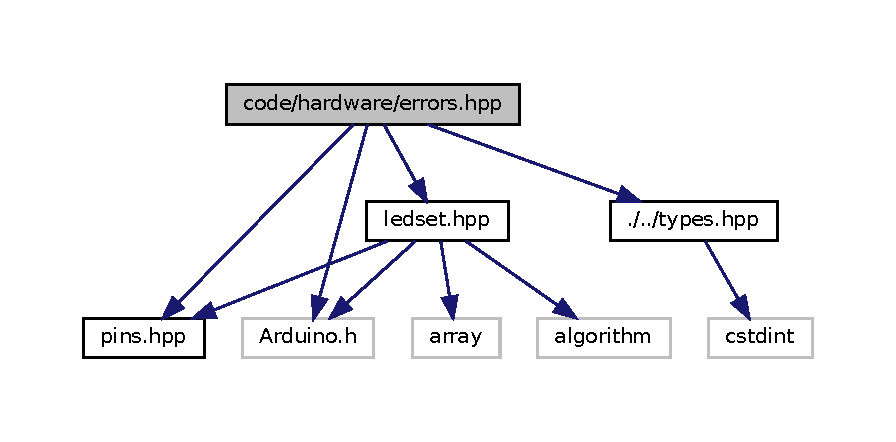
\includegraphics[width=350pt]{errors_8hpp__incl}
\end{center}
\end{figure}
This graph shows which files directly or indirectly include this file\+:\nopagebreak
\begin{figure}[H]
\begin{center}
\leavevmode
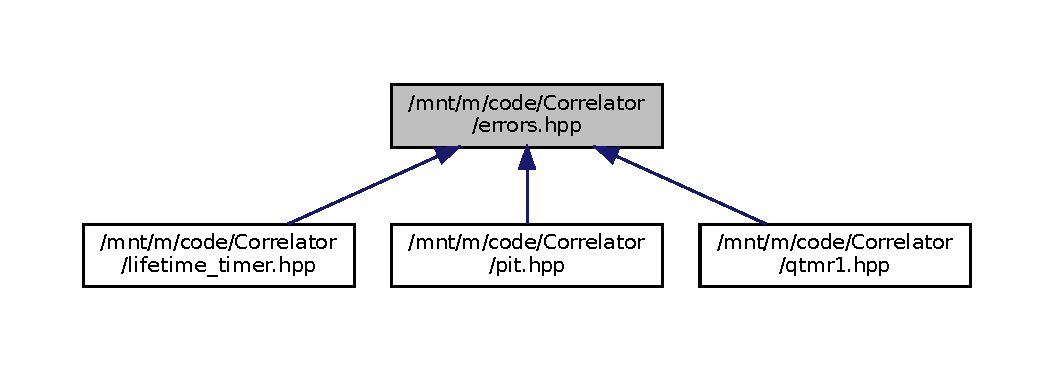
\includegraphics[width=350pt]{errors_8hpp__dep__incl}
\end{center}
\end{figure}
\subsection*{Classes}
\begin{DoxyCompactItemize}
\item 
class \hyperlink{classErrors}{Errors}
\end{DoxyCompactItemize}
\subsection*{Macros}
\begin{DoxyCompactItemize}
\item 
\#define \hyperlink{errors_8hpp_a0eb326048ed31037a6e5ec5634a6202e}{T\+E\+E\+N\+S\+Y\+\_\+\+M\+A\+X\+\_\+\+A\+L\+L\+O\+C\+A\+T\+I\+ON}~125000
\begin{DoxyCompactList}\small\item\em This file contain the Common Error Codes for Software-\/\+Hardware Interface. It defines the {\ttfamily Error\+\_\+t} and namespace {\ttfamily \hyperlink{classErrors}{Errors}} that are used to handle the errors and interact with the L\+ED dashboard. \end{DoxyCompactList}\end{DoxyCompactItemize}
\subsection*{Enumerations}
\begin{DoxyCompactItemize}
\item 
enum \hyperlink{errors_8hpp_a4e8c0d09726859e3d3369c0da5a1aa7f}{Error\+\_\+t} \{ \newline
\hyperlink{errors_8hpp_a4e8c0d09726859e3d3369c0da5a1aa7fa505a83f220c02df2f85c3810cd9ceb38}{Error\+\_\+t\+::\+Success} = 0, 
\hyperlink{errors_8hpp_a4e8c0d09726859e3d3369c0da5a1aa7fa8347bab2e74e4a640d76c916306a1a36}{Error\+\_\+t\+::\+Counter\+\_\+\+Overflow}, 
\hyperlink{errors_8hpp_a4e8c0d09726859e3d3369c0da5a1aa7fa02b02f5e5e61f24acdd91338b95997da}{Error\+\_\+t\+::\+Counter\+\_\+\+Underflow}, 
\hyperlink{errors_8hpp_a4e8c0d09726859e3d3369c0da5a1aa7fabe5edab59de4ea30531374e506b03822}{Error\+\_\+t\+::\+Precision}, 
\newline
\hyperlink{errors_8hpp_a4e8c0d09726859e3d3369c0da5a1aa7fa7e748bca7005cc737bad51b247997421}{Error\+\_\+t\+::\+Input\+\_\+\+Validation}, 
\hyperlink{errors_8hpp_a4e8c0d09726859e3d3369c0da5a1aa7fac7e40b9218d101cde2dc4c43b9fed0fe}{Error\+\_\+t\+::\+Generic\+\_\+\+Error}
 \}\begin{DoxyCompactList}\small\item\em Enumarates the error codes thrown by the different modules. \end{DoxyCompactList}
\end{DoxyCompactItemize}


\subsection{Macro Definition Documentation}
\mbox{\Hypertarget{errors_8hpp_a0eb326048ed31037a6e5ec5634a6202e}\label{errors_8hpp_a0eb326048ed31037a6e5ec5634a6202e}} 
\index{errors.\+hpp@{errors.\+hpp}!T\+E\+E\+N\+S\+Y\+\_\+\+M\+A\+X\+\_\+\+A\+L\+L\+O\+C\+A\+T\+I\+ON@{T\+E\+E\+N\+S\+Y\+\_\+\+M\+A\+X\+\_\+\+A\+L\+L\+O\+C\+A\+T\+I\+ON}}
\index{T\+E\+E\+N\+S\+Y\+\_\+\+M\+A\+X\+\_\+\+A\+L\+L\+O\+C\+A\+T\+I\+ON@{T\+E\+E\+N\+S\+Y\+\_\+\+M\+A\+X\+\_\+\+A\+L\+L\+O\+C\+A\+T\+I\+ON}!errors.\+hpp@{errors.\+hpp}}
\subsubsection{\texorpdfstring{T\+E\+E\+N\+S\+Y\+\_\+\+M\+A\+X\+\_\+\+A\+L\+L\+O\+C\+A\+T\+I\+ON}{TEENSY\_MAX\_ALLOCATION}}
{\footnotesize\ttfamily \#define T\+E\+E\+N\+S\+Y\+\_\+\+M\+A\+X\+\_\+\+A\+L\+L\+O\+C\+A\+T\+I\+ON~125000}



This file contain the Common Error Codes for Software-\/\+Hardware Interface. It defines the {\ttfamily Error\+\_\+t} and namespace {\ttfamily \hyperlink{classErrors}{Errors}} that are used to handle the errors and interact with the L\+ED dashboard. 

\begin{DoxyAuthor}{Author}
Yatharth Bhasin (github → yatharthb97) Maximum Allocations of 32-\/bit integers allowed on the microcontroller Teensy. 
\end{DoxyAuthor}


\subsection{Enumeration Type Documentation}
\mbox{\Hypertarget{errors_8hpp_a4e8c0d09726859e3d3369c0da5a1aa7f}\label{errors_8hpp_a4e8c0d09726859e3d3369c0da5a1aa7f}} 
\index{errors.\+hpp@{errors.\+hpp}!Error\+\_\+t@{Error\+\_\+t}}
\index{Error\+\_\+t@{Error\+\_\+t}!errors.\+hpp@{errors.\+hpp}}
\subsubsection{\texorpdfstring{Error\+\_\+t}{Error\_t}}
{\footnotesize\ttfamily enum \hyperlink{errors_8hpp_a4e8c0d09726859e3d3369c0da5a1aa7f}{Error\+\_\+t}\hspace{0.3cm}{\ttfamily [strong]}}



Enumarates the error codes thrown by the different modules. 

\begin{DoxyEnumFields}{Enumerator}
\raisebox{\heightof{T}}[0pt][0pt]{\index{Success@{Success}!errors.\+hpp@{errors.\+hpp}}\index{errors.\+hpp@{errors.\+hpp}!Success@{Success}}}\mbox{\Hypertarget{errors_8hpp_a4e8c0d09726859e3d3369c0da5a1aa7fa505a83f220c02df2f85c3810cd9ceb38}\label{errors_8hpp_a4e8c0d09726859e3d3369c0da5a1aa7fa505a83f220c02df2f85c3810cd9ceb38}} 
Success&No error. \\
\hline

\raisebox{\heightof{T}}[0pt][0pt]{\index{Counter\+\_\+\+Overflow@{Counter\+\_\+\+Overflow}!errors.\+hpp@{errors.\+hpp}}\index{errors.\+hpp@{errors.\+hpp}!Counter\+\_\+\+Overflow@{Counter\+\_\+\+Overflow}}}\mbox{\Hypertarget{errors_8hpp_a4e8c0d09726859e3d3369c0da5a1aa7fa8347bab2e74e4a640d76c916306a1a36}\label{errors_8hpp_a4e8c0d09726859e3d3369c0da5a1aa7fa8347bab2e74e4a640d76c916306a1a36}} 
Counter\+\_\+\+Overflow&Passed Value caused a counter overflow. \\
\hline

\raisebox{\heightof{T}}[0pt][0pt]{\index{Counter\+\_\+\+Underflow@{Counter\+\_\+\+Underflow}!errors.\+hpp@{errors.\+hpp}}\index{errors.\+hpp@{errors.\+hpp}!Counter\+\_\+\+Underflow@{Counter\+\_\+\+Underflow}}}\mbox{\Hypertarget{errors_8hpp_a4e8c0d09726859e3d3369c0da5a1aa7fa02b02f5e5e61f24acdd91338b95997da}\label{errors_8hpp_a4e8c0d09726859e3d3369c0da5a1aa7fa02b02f5e5e61f24acdd91338b95997da}} 
Counter\+\_\+\+Underflow&Passed Value caused a counter underflow. \\
\hline

\raisebox{\heightof{T}}[0pt][0pt]{\index{Precision@{Precision}!errors.\+hpp@{errors.\+hpp}}\index{errors.\+hpp@{errors.\+hpp}!Precision@{Precision}}}\mbox{\Hypertarget{errors_8hpp_a4e8c0d09726859e3d3369c0da5a1aa7fabe5edab59de4ea30531374e506b03822}\label{errors_8hpp_a4e8c0d09726859e3d3369c0da5a1aa7fabe5edab59de4ea30531374e506b03822}} 
Precision&Error generated when difference due to finite resolution is greater than acceptable. \\
\hline

\raisebox{\heightof{T}}[0pt][0pt]{\index{Input\+\_\+\+Validation@{Input\+\_\+\+Validation}!errors.\+hpp@{errors.\+hpp}}\index{errors.\+hpp@{errors.\+hpp}!Input\+\_\+\+Validation@{Input\+\_\+\+Validation}}}\mbox{\Hypertarget{errors_8hpp_a4e8c0d09726859e3d3369c0da5a1aa7fa7e748bca7005cc737bad51b247997421}\label{errors_8hpp_a4e8c0d09726859e3d3369c0da5a1aa7fa7e748bca7005cc737bad51b247997421}} 
Input\+\_\+\+Validation&Input validation failed. \\
\hline

\raisebox{\heightof{T}}[0pt][0pt]{\index{Generic\+\_\+\+Error@{Generic\+\_\+\+Error}!errors.\+hpp@{errors.\+hpp}}\index{errors.\+hpp@{errors.\+hpp}!Generic\+\_\+\+Error@{Generic\+\_\+\+Error}}}\mbox{\Hypertarget{errors_8hpp_a4e8c0d09726859e3d3369c0da5a1aa7fac7e40b9218d101cde2dc4c43b9fed0fe}\label{errors_8hpp_a4e8c0d09726859e3d3369c0da5a1aa7fac7e40b9218d101cde2dc4c43b9fed0fe}} 
Generic\+\_\+\+Error&Only here for development and debugging. \\
\hline

\end{DoxyEnumFields}

\hypertarget{ledset_8hpp}{}\section{code/hardware/ledset.hpp File Reference}
\label{ledset_8hpp}\index{code/hardware/ledset.\+hpp@{code/hardware/ledset.\+hpp}}
{\ttfamily \#include $<$Arduino.\+h$>$}\newline
{\ttfamily \#include $<$algorithm$>$}\newline
{\ttfamily \#include \char`\"{}pins.\+hpp\char`\"{}}\newline
{\ttfamily \#include $<$array$>$}\newline
{\ttfamily \#include $<$initializer\+\_\+list$>$}\newline
Include dependency graph for ledset.\+hpp\+:\nopagebreak
\begin{figure}[H]
\begin{center}
\leavevmode
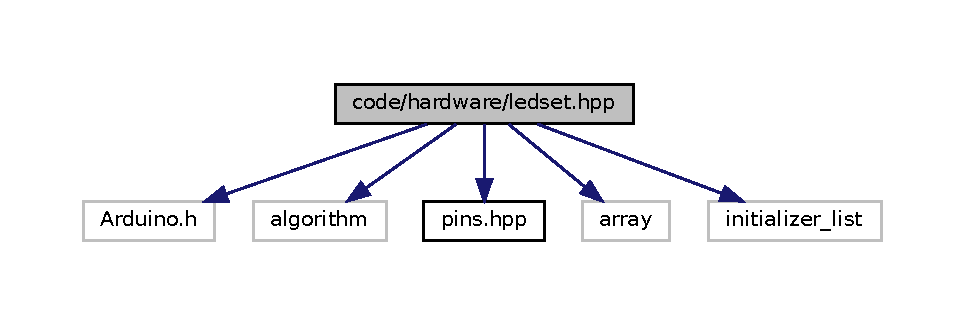
\includegraphics[width=350pt]{ledset_8hpp__incl}
\end{center}
\end{figure}
This graph shows which files directly or indirectly include this file\+:\nopagebreak
\begin{figure}[H]
\begin{center}
\leavevmode
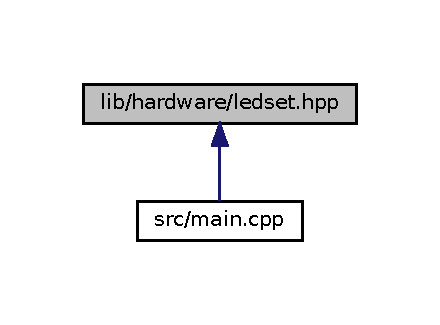
\includegraphics[width=350pt]{ledset_8hpp__dep__incl}
\end{center}
\end{figure}
\subsection*{Classes}
\begin{DoxyCompactItemize}
\item 
class \hyperlink{classLEDSet}{L\+E\+D\+Set$<$ S\+E\+T\+\_\+\+S\+I\+Z\+E $>$}
\end{DoxyCompactItemize}

\hypertarget{lifetime__timer_8hpp}{}\section{/mnt/m/code/\+Correlator/lifetime\+\_\+timer.hpp File Reference}
\label{lifetime__timer_8hpp}\index{/mnt/m/code/\+Correlator/lifetime\+\_\+timer.\+hpp@{/mnt/m/code/\+Correlator/lifetime\+\_\+timer.\+hpp}}
{\ttfamily \#include \char`\"{}errors.\+hpp\char`\"{}}\newline
Include dependency graph for lifetime\+\_\+timer.\+hpp\+:
\nopagebreak
\begin{figure}[H]
\begin{center}
\leavevmode
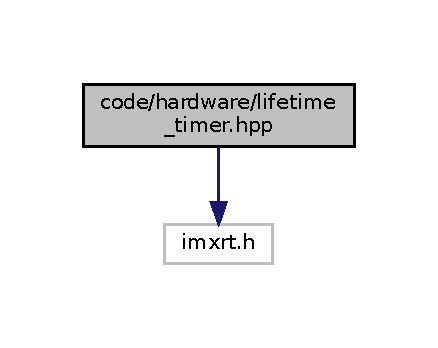
\includegraphics[width=210pt]{lifetime__timer_8hpp__incl}
\end{center}
\end{figure}
\subsection*{Classes}
\begin{DoxyCompactItemize}
\item 
class \hyperlink{classPIT__LifetimeTimer}{P\+I\+T\+\_\+\+Lifetime\+Timer}
\begin{DoxyCompactList}\small\item\em Interface for using the \char`\"{}\+Life Time T\+Imer\char`\"{} functionality of the Periodic Interrut Timer on Teensy 4.\+x microcontrollers. The module uses Channel 0 and 1 of the 4 P\+IT channels. \end{DoxyCompactList}\end{DoxyCompactItemize}

\hypertarget{pins_8hpp}{}\section{code/hardware/pins.hpp File Reference}
\label{pins_8hpp}\index{code/hardware/pins.\+hpp@{code/hardware/pins.\+hpp}}
This graph shows which files directly or indirectly include this file\+:\nopagebreak
\begin{figure}[H]
\begin{center}
\leavevmode
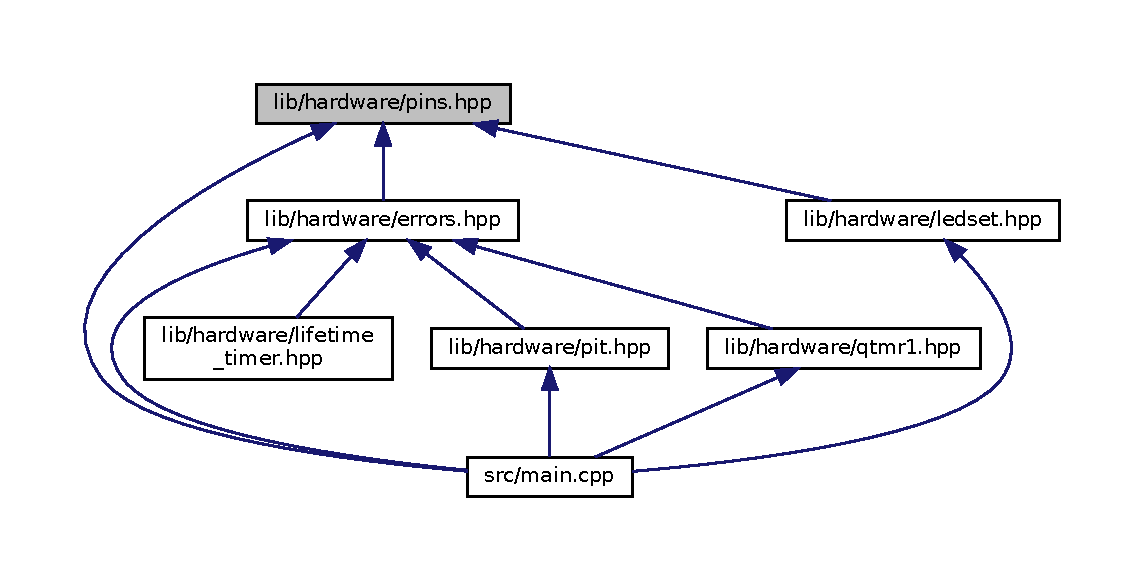
\includegraphics[width=350pt]{pins_8hpp__dep__incl}
\end{center}
\end{figure}
\subsection*{Variables}
\begin{DoxyCompactItemize}
\item 
const int \hyperlink{pins_8hpp_a735f426a390e22c0050b964328c5e06f}{L\+E\+D\+\_\+\+R\+ED} = 41
\item 
const int \hyperlink{pins_8hpp_a8046eca6ddcbe578777cfde489622a13}{L\+E\+D\+\_\+\+B\+L\+UE} = 40
\item 
const int \hyperlink{pins_8hpp_af338796c804fbfe2e9fd4d249e3c5004}{L\+E\+D\+\_\+\+Y\+E\+L\+L\+OW} = 22
\item 
const int \hyperlink{pins_8hpp_a1be903f86639d50fb6ed02a0dbbe0e2c}{L\+E\+D\+\_\+\+W\+H\+I\+TE} = 23
\item 
const int \hyperlink{pins_8hpp_a8d7df4222b2fde6205bebffc5a0ae070}{L\+E\+D\+\_\+\+G\+R\+E\+EN} = 24
\item 
const int \hyperlink{pins_8hpp_a6a5a6d5ec94efcbf2c8bffa0b660f013}{S\+A\+F\+E\+\_\+\+I\+N\+P\+U\+T\+\_\+\+D\+U\+M\+P\+\_\+\+P\+IN} = 0
\item 
const int \hyperlink{pins_8hpp_a2b2fb4f846b45d396215a25f949a1bc7}{S\+A\+F\+E\+\_\+\+O\+U\+T\+P\+U\+T\+\_\+\+D\+U\+M\+P\+\_\+\+P\+IN} = 0
\item 
const int \hyperlink{pins_8hpp_a5017daf6b9fb9330e86878ec983ed163}{T\+T\+L\+\_\+\+C\+\_\+\+P\+U\+L\+S\+E\+\_\+\+I\+N\+P\+U\+T\+\_\+\+P\+IN} = 10
\item 
const int \hyperlink{pins_8hpp_a01ff5c1b8f46ca9504e840c5aaf9fd64}{E\+R\+\_\+\+P\+R\+E\+C\+I\+S\+I\+O\+N\+\_\+\+P\+IN} = \hyperlink{pins_8hpp_a8046eca6ddcbe578777cfde489622a13}{L\+E\+D\+\_\+\+B\+L\+UE}
\item 
const int \hyperlink{pins_8hpp_ae73bc7e4372631b754daf933169b2a16}{E\+R\+\_\+\+O\+V\+E\+R\+F\+L\+O\+W\+\_\+\+P\+IN} = \hyperlink{pins_8hpp_a1be903f86639d50fb6ed02a0dbbe0e2c}{L\+E\+D\+\_\+\+W\+H\+I\+TE}
\item 
const int \hyperlink{pins_8hpp_a3bf66a7f687091434a704c61863c3141}{E\+R\+\_\+\+I\+N\+P\+U\+T\+\_\+\+V\+A\+L\+I\+D\+A\+T\+I\+ON} = \hyperlink{pins_8hpp_a735f426a390e22c0050b964328c5e06f}{L\+E\+D\+\_\+\+R\+ED}
\item 
const int \hyperlink{pins_8hpp_a3bceb7a516452849c8b6292b69e4fb71}{S\+E\+T\+U\+P\+\_\+\+L\+ED} = \hyperlink{pins_8hpp_a735f426a390e22c0050b964328c5e06f}{L\+E\+D\+\_\+\+R\+ED}
\item 
const int \hyperlink{pins_8hpp_a1c1c13275493f645825a60c5710264e5}{L\+O\+O\+P\+\_\+\+L\+ED} = \hyperlink{pins_8hpp_a8d7df4222b2fde6205bebffc5a0ae070}{L\+E\+D\+\_\+\+G\+R\+E\+EN}
\end{DoxyCompactItemize}


\subsection{Variable Documentation}
\mbox{\Hypertarget{pins_8hpp_a3bf66a7f687091434a704c61863c3141}\label{pins_8hpp_a3bf66a7f687091434a704c61863c3141}} 
\index{pins.\+hpp@{pins.\+hpp}!E\+R\+\_\+\+I\+N\+P\+U\+T\+\_\+\+V\+A\+L\+I\+D\+A\+T\+I\+ON@{E\+R\+\_\+\+I\+N\+P\+U\+T\+\_\+\+V\+A\+L\+I\+D\+A\+T\+I\+ON}}
\index{E\+R\+\_\+\+I\+N\+P\+U\+T\+\_\+\+V\+A\+L\+I\+D\+A\+T\+I\+ON@{E\+R\+\_\+\+I\+N\+P\+U\+T\+\_\+\+V\+A\+L\+I\+D\+A\+T\+I\+ON}!pins.\+hpp@{pins.\+hpp}}
\subsubsection{\texorpdfstring{E\+R\+\_\+\+I\+N\+P\+U\+T\+\_\+\+V\+A\+L\+I\+D\+A\+T\+I\+ON}{ER\_INPUT\_VALIDATION}}
{\footnotesize\ttfamily const int E\+R\+\_\+\+I\+N\+P\+U\+T\+\_\+\+V\+A\+L\+I\+D\+A\+T\+I\+ON = \hyperlink{pins_8hpp_a735f426a390e22c0050b964328c5e06f}{L\+E\+D\+\_\+\+R\+ED}}

\mbox{\Hypertarget{pins_8hpp_ae73bc7e4372631b754daf933169b2a16}\label{pins_8hpp_ae73bc7e4372631b754daf933169b2a16}} 
\index{pins.\+hpp@{pins.\+hpp}!E\+R\+\_\+\+O\+V\+E\+R\+F\+L\+O\+W\+\_\+\+P\+IN@{E\+R\+\_\+\+O\+V\+E\+R\+F\+L\+O\+W\+\_\+\+P\+IN}}
\index{E\+R\+\_\+\+O\+V\+E\+R\+F\+L\+O\+W\+\_\+\+P\+IN@{E\+R\+\_\+\+O\+V\+E\+R\+F\+L\+O\+W\+\_\+\+P\+IN}!pins.\+hpp@{pins.\+hpp}}
\subsubsection{\texorpdfstring{E\+R\+\_\+\+O\+V\+E\+R\+F\+L\+O\+W\+\_\+\+P\+IN}{ER\_OVERFLOW\_PIN}}
{\footnotesize\ttfamily const int E\+R\+\_\+\+O\+V\+E\+R\+F\+L\+O\+W\+\_\+\+P\+IN = \hyperlink{pins_8hpp_a1be903f86639d50fb6ed02a0dbbe0e2c}{L\+E\+D\+\_\+\+W\+H\+I\+TE}}

\mbox{\Hypertarget{pins_8hpp_a01ff5c1b8f46ca9504e840c5aaf9fd64}\label{pins_8hpp_a01ff5c1b8f46ca9504e840c5aaf9fd64}} 
\index{pins.\+hpp@{pins.\+hpp}!E\+R\+\_\+\+P\+R\+E\+C\+I\+S\+I\+O\+N\+\_\+\+P\+IN@{E\+R\+\_\+\+P\+R\+E\+C\+I\+S\+I\+O\+N\+\_\+\+P\+IN}}
\index{E\+R\+\_\+\+P\+R\+E\+C\+I\+S\+I\+O\+N\+\_\+\+P\+IN@{E\+R\+\_\+\+P\+R\+E\+C\+I\+S\+I\+O\+N\+\_\+\+P\+IN}!pins.\+hpp@{pins.\+hpp}}
\subsubsection{\texorpdfstring{E\+R\+\_\+\+P\+R\+E\+C\+I\+S\+I\+O\+N\+\_\+\+P\+IN}{ER\_PRECISION\_PIN}}
{\footnotesize\ttfamily const int E\+R\+\_\+\+P\+R\+E\+C\+I\+S\+I\+O\+N\+\_\+\+P\+IN = \hyperlink{pins_8hpp_a8046eca6ddcbe578777cfde489622a13}{L\+E\+D\+\_\+\+B\+L\+UE}}

\mbox{\Hypertarget{pins_8hpp_a8046eca6ddcbe578777cfde489622a13}\label{pins_8hpp_a8046eca6ddcbe578777cfde489622a13}} 
\index{pins.\+hpp@{pins.\+hpp}!L\+E\+D\+\_\+\+B\+L\+UE@{L\+E\+D\+\_\+\+B\+L\+UE}}
\index{L\+E\+D\+\_\+\+B\+L\+UE@{L\+E\+D\+\_\+\+B\+L\+UE}!pins.\+hpp@{pins.\+hpp}}
\subsubsection{\texorpdfstring{L\+E\+D\+\_\+\+B\+L\+UE}{LED\_BLUE}}
{\footnotesize\ttfamily const int L\+E\+D\+\_\+\+B\+L\+UE = 40}

\mbox{\Hypertarget{pins_8hpp_a8d7df4222b2fde6205bebffc5a0ae070}\label{pins_8hpp_a8d7df4222b2fde6205bebffc5a0ae070}} 
\index{pins.\+hpp@{pins.\+hpp}!L\+E\+D\+\_\+\+G\+R\+E\+EN@{L\+E\+D\+\_\+\+G\+R\+E\+EN}}
\index{L\+E\+D\+\_\+\+G\+R\+E\+EN@{L\+E\+D\+\_\+\+G\+R\+E\+EN}!pins.\+hpp@{pins.\+hpp}}
\subsubsection{\texorpdfstring{L\+E\+D\+\_\+\+G\+R\+E\+EN}{LED\_GREEN}}
{\footnotesize\ttfamily const int L\+E\+D\+\_\+\+G\+R\+E\+EN = 24}

\mbox{\Hypertarget{pins_8hpp_a735f426a390e22c0050b964328c5e06f}\label{pins_8hpp_a735f426a390e22c0050b964328c5e06f}} 
\index{pins.\+hpp@{pins.\+hpp}!L\+E\+D\+\_\+\+R\+ED@{L\+E\+D\+\_\+\+R\+ED}}
\index{L\+E\+D\+\_\+\+R\+ED@{L\+E\+D\+\_\+\+R\+ED}!pins.\+hpp@{pins.\+hpp}}
\subsubsection{\texorpdfstring{L\+E\+D\+\_\+\+R\+ED}{LED\_RED}}
{\footnotesize\ttfamily const int L\+E\+D\+\_\+\+R\+ED = 41}

\mbox{\Hypertarget{pins_8hpp_a1be903f86639d50fb6ed02a0dbbe0e2c}\label{pins_8hpp_a1be903f86639d50fb6ed02a0dbbe0e2c}} 
\index{pins.\+hpp@{pins.\+hpp}!L\+E\+D\+\_\+\+W\+H\+I\+TE@{L\+E\+D\+\_\+\+W\+H\+I\+TE}}
\index{L\+E\+D\+\_\+\+W\+H\+I\+TE@{L\+E\+D\+\_\+\+W\+H\+I\+TE}!pins.\+hpp@{pins.\+hpp}}
\subsubsection{\texorpdfstring{L\+E\+D\+\_\+\+W\+H\+I\+TE}{LED\_WHITE}}
{\footnotesize\ttfamily const int L\+E\+D\+\_\+\+W\+H\+I\+TE = 23}

\mbox{\Hypertarget{pins_8hpp_af338796c804fbfe2e9fd4d249e3c5004}\label{pins_8hpp_af338796c804fbfe2e9fd4d249e3c5004}} 
\index{pins.\+hpp@{pins.\+hpp}!L\+E\+D\+\_\+\+Y\+E\+L\+L\+OW@{L\+E\+D\+\_\+\+Y\+E\+L\+L\+OW}}
\index{L\+E\+D\+\_\+\+Y\+E\+L\+L\+OW@{L\+E\+D\+\_\+\+Y\+E\+L\+L\+OW}!pins.\+hpp@{pins.\+hpp}}
\subsubsection{\texorpdfstring{L\+E\+D\+\_\+\+Y\+E\+L\+L\+OW}{LED\_YELLOW}}
{\footnotesize\ttfamily const int L\+E\+D\+\_\+\+Y\+E\+L\+L\+OW = 22}

\mbox{\Hypertarget{pins_8hpp_a1c1c13275493f645825a60c5710264e5}\label{pins_8hpp_a1c1c13275493f645825a60c5710264e5}} 
\index{pins.\+hpp@{pins.\+hpp}!L\+O\+O\+P\+\_\+\+L\+ED@{L\+O\+O\+P\+\_\+\+L\+ED}}
\index{L\+O\+O\+P\+\_\+\+L\+ED@{L\+O\+O\+P\+\_\+\+L\+ED}!pins.\+hpp@{pins.\+hpp}}
\subsubsection{\texorpdfstring{L\+O\+O\+P\+\_\+\+L\+ED}{LOOP\_LED}}
{\footnotesize\ttfamily const int L\+O\+O\+P\+\_\+\+L\+ED = \hyperlink{pins_8hpp_a8d7df4222b2fde6205bebffc5a0ae070}{L\+E\+D\+\_\+\+G\+R\+E\+EN}}

\mbox{\Hypertarget{pins_8hpp_a6a5a6d5ec94efcbf2c8bffa0b660f013}\label{pins_8hpp_a6a5a6d5ec94efcbf2c8bffa0b660f013}} 
\index{pins.\+hpp@{pins.\+hpp}!S\+A\+F\+E\+\_\+\+I\+N\+P\+U\+T\+\_\+\+D\+U\+M\+P\+\_\+\+P\+IN@{S\+A\+F\+E\+\_\+\+I\+N\+P\+U\+T\+\_\+\+D\+U\+M\+P\+\_\+\+P\+IN}}
\index{S\+A\+F\+E\+\_\+\+I\+N\+P\+U\+T\+\_\+\+D\+U\+M\+P\+\_\+\+P\+IN@{S\+A\+F\+E\+\_\+\+I\+N\+P\+U\+T\+\_\+\+D\+U\+M\+P\+\_\+\+P\+IN}!pins.\+hpp@{pins.\+hpp}}
\subsubsection{\texorpdfstring{S\+A\+F\+E\+\_\+\+I\+N\+P\+U\+T\+\_\+\+D\+U\+M\+P\+\_\+\+P\+IN}{SAFE\_INPUT\_DUMP\_PIN}}
{\footnotesize\ttfamily const int S\+A\+F\+E\+\_\+\+I\+N\+P\+U\+T\+\_\+\+D\+U\+M\+P\+\_\+\+P\+IN = 0}

\mbox{\Hypertarget{pins_8hpp_a2b2fb4f846b45d396215a25f949a1bc7}\label{pins_8hpp_a2b2fb4f846b45d396215a25f949a1bc7}} 
\index{pins.\+hpp@{pins.\+hpp}!S\+A\+F\+E\+\_\+\+O\+U\+T\+P\+U\+T\+\_\+\+D\+U\+M\+P\+\_\+\+P\+IN@{S\+A\+F\+E\+\_\+\+O\+U\+T\+P\+U\+T\+\_\+\+D\+U\+M\+P\+\_\+\+P\+IN}}
\index{S\+A\+F\+E\+\_\+\+O\+U\+T\+P\+U\+T\+\_\+\+D\+U\+M\+P\+\_\+\+P\+IN@{S\+A\+F\+E\+\_\+\+O\+U\+T\+P\+U\+T\+\_\+\+D\+U\+M\+P\+\_\+\+P\+IN}!pins.\+hpp@{pins.\+hpp}}
\subsubsection{\texorpdfstring{S\+A\+F\+E\+\_\+\+O\+U\+T\+P\+U\+T\+\_\+\+D\+U\+M\+P\+\_\+\+P\+IN}{SAFE\_OUTPUT\_DUMP\_PIN}}
{\footnotesize\ttfamily const int S\+A\+F\+E\+\_\+\+O\+U\+T\+P\+U\+T\+\_\+\+D\+U\+M\+P\+\_\+\+P\+IN = 0}

\mbox{\Hypertarget{pins_8hpp_a3bceb7a516452849c8b6292b69e4fb71}\label{pins_8hpp_a3bceb7a516452849c8b6292b69e4fb71}} 
\index{pins.\+hpp@{pins.\+hpp}!S\+E\+T\+U\+P\+\_\+\+L\+ED@{S\+E\+T\+U\+P\+\_\+\+L\+ED}}
\index{S\+E\+T\+U\+P\+\_\+\+L\+ED@{S\+E\+T\+U\+P\+\_\+\+L\+ED}!pins.\+hpp@{pins.\+hpp}}
\subsubsection{\texorpdfstring{S\+E\+T\+U\+P\+\_\+\+L\+ED}{SETUP\_LED}}
{\footnotesize\ttfamily const int S\+E\+T\+U\+P\+\_\+\+L\+ED = \hyperlink{pins_8hpp_a735f426a390e22c0050b964328c5e06f}{L\+E\+D\+\_\+\+R\+ED}}

\mbox{\Hypertarget{pins_8hpp_a5017daf6b9fb9330e86878ec983ed163}\label{pins_8hpp_a5017daf6b9fb9330e86878ec983ed163}} 
\index{pins.\+hpp@{pins.\+hpp}!T\+T\+L\+\_\+\+C\+\_\+\+P\+U\+L\+S\+E\+\_\+\+I\+N\+P\+U\+T\+\_\+\+P\+IN@{T\+T\+L\+\_\+\+C\+\_\+\+P\+U\+L\+S\+E\+\_\+\+I\+N\+P\+U\+T\+\_\+\+P\+IN}}
\index{T\+T\+L\+\_\+\+C\+\_\+\+P\+U\+L\+S\+E\+\_\+\+I\+N\+P\+U\+T\+\_\+\+P\+IN@{T\+T\+L\+\_\+\+C\+\_\+\+P\+U\+L\+S\+E\+\_\+\+I\+N\+P\+U\+T\+\_\+\+P\+IN}!pins.\+hpp@{pins.\+hpp}}
\subsubsection{\texorpdfstring{T\+T\+L\+\_\+\+C\+\_\+\+P\+U\+L\+S\+E\+\_\+\+I\+N\+P\+U\+T\+\_\+\+P\+IN}{TTL\_C\_PULSE\_INPUT\_PIN}}
{\footnotesize\ttfamily const int T\+T\+L\+\_\+\+C\+\_\+\+P\+U\+L\+S\+E\+\_\+\+I\+N\+P\+U\+T\+\_\+\+P\+IN = 10}


\hypertarget{pit_8hpp}{}\section{/mnt/m/code/\+Correlator/pit.hpp File Reference}
\label{pit_8hpp}\index{/mnt/m/code/\+Correlator/pit.\+hpp@{/mnt/m/code/\+Correlator/pit.\+hpp}}
{\ttfamily \#include \char`\"{}errors.\+hpp\char`\"{}}\newline
Include dependency graph for pit.\+hpp\+:\nopagebreak
\begin{figure}[H]
\begin{center}
\leavevmode
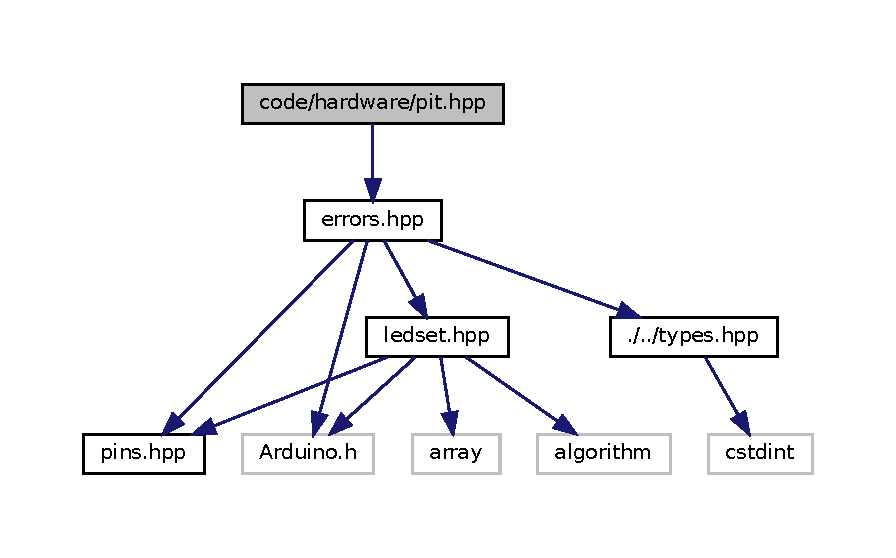
\includegraphics[width=210pt]{pit_8hpp__incl}
\end{center}
\end{figure}
\subsection*{Classes}
\begin{DoxyCompactItemize}
\item 
class \hyperlink{classPITController}{P\+I\+T\+Controller$<$ Ch\+I\+D $>$}
\begin{DoxyCompactList}\small\item\em Interface for P\+IT timers on Teensy 4.\+x microcontrollers. \end{DoxyCompactList}\end{DoxyCompactItemize}

\hypertarget{qtmr1_8hpp}{}\section{code/hardware/qtmr1.hpp File Reference}
\label{qtmr1_8hpp}\index{code/hardware/qtmr1.\+hpp@{code/hardware/qtmr1.\+hpp}}
{\ttfamily \#include \char`\"{}errors.\+hpp\char`\"{}}\newline
Include dependency graph for qtmr1.\+hpp\+:\nopagebreak
\begin{figure}[H]
\begin{center}
\leavevmode
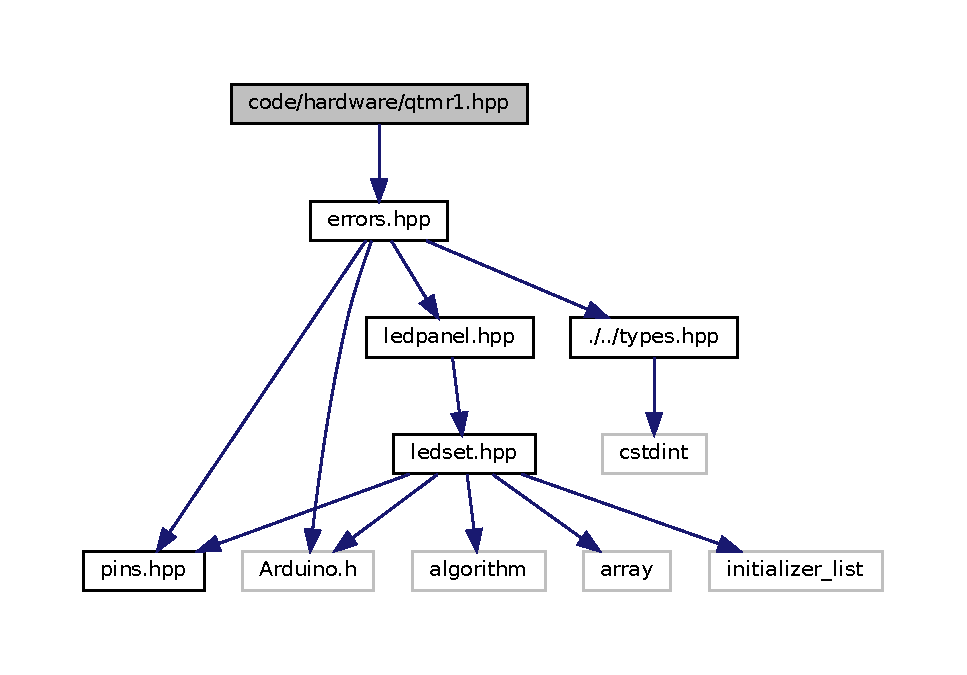
\includegraphics[width=350pt]{d5/d22/qtmr1_8hpp__incl}
\end{center}
\end{figure}
This graph shows which files directly or indirectly include this file\+:
\nopagebreak
\begin{figure}[H]
\begin{center}
\leavevmode
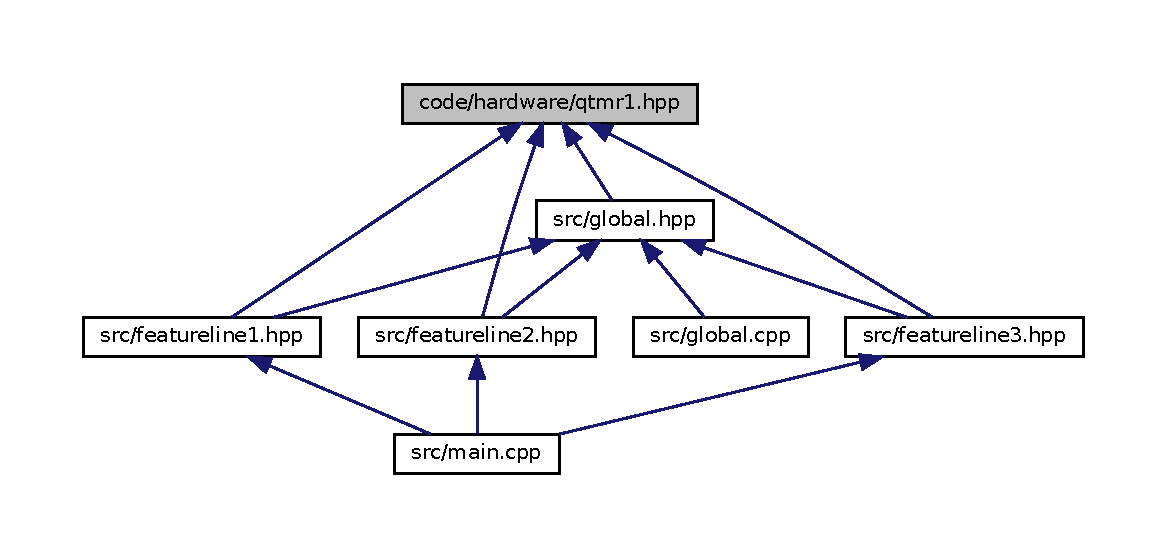
\includegraphics[width=350pt]{de/dea/qtmr1_8hpp__dep__incl}
\end{center}
\end{figure}
\subsection*{Classes}
\begin{DoxyCompactItemize}
\item 
class \hyperlink{classTMR1Controller}{T\+M\+R1\+Controller}
\begin{DoxyCompactList}\small\item\em Templated interface for Quad Timer 1 channels for Gate Counting. The module uses the macro {\ttfamily \+\_\+\+T\+M\+R1\+\_\+\+C\+O\+N\+T\+R\+O\+L\+L\+E\+R\+\_\+\+C\+H\+\_\+} to identify the main channel and then assigns the next channel\textquotesingle{}s ({\itshape T\+M\+R1\+\_\+\+C\+O\+N\+T\+R\+O\+L\+L\+E\+R\+\_\+\+CH} + 1) external pin to the {\itshape T\+M\+R1\+\_\+\+C\+O\+N\+T\+R\+O\+L\+L\+E\+R\+\_\+\+CH} as the \char`\"{}\+Capture Pin\char`\"{} or the \char`\"{}\+Secondary Count Source\char`\"{}. \end{DoxyCompactList}\end{DoxyCompactItemize}
\subsection*{Macros}
\begin{DoxyCompactItemize}
\item 
\#define \hyperlink{qtmr1_8hpp_a9b1e0ba00a31105b8b486365043a4cd2}{\+\_\+\+T\+M\+R1\+\_\+\+C\+O\+N\+T\+R\+O\+L\+L\+E\+R\+\_\+\+C\+H\+\_\+}~0
\end{DoxyCompactItemize}


\subsection{Macro Definition Documentation}
\mbox{\Hypertarget{qtmr1_8hpp_a9b1e0ba00a31105b8b486365043a4cd2}\label{qtmr1_8hpp_a9b1e0ba00a31105b8b486365043a4cd2}} 
\index{qtmr1.\+hpp@{qtmr1.\+hpp}!\+\_\+\+T\+M\+R1\+\_\+\+C\+O\+N\+T\+R\+O\+L\+L\+E\+R\+\_\+\+C\+H\+\_\+@{\+\_\+\+T\+M\+R1\+\_\+\+C\+O\+N\+T\+R\+O\+L\+L\+E\+R\+\_\+\+C\+H\+\_\+}}
\index{\+\_\+\+T\+M\+R1\+\_\+\+C\+O\+N\+T\+R\+O\+L\+L\+E\+R\+\_\+\+C\+H\+\_\+@{\+\_\+\+T\+M\+R1\+\_\+\+C\+O\+N\+T\+R\+O\+L\+L\+E\+R\+\_\+\+C\+H\+\_\+}!qtmr1.\+hpp@{qtmr1.\+hpp}}
\subsubsection{\texorpdfstring{\+\_\+\+T\+M\+R1\+\_\+\+C\+O\+N\+T\+R\+O\+L\+L\+E\+R\+\_\+\+C\+H\+\_\+}{\_TMR1\_CONTROLLER\_CH\_}}
{\footnotesize\ttfamily \#define \+\_\+\+T\+M\+R1\+\_\+\+C\+O\+N\+T\+R\+O\+L\+L\+E\+R\+\_\+\+C\+H\+\_\+~0}


\hypertarget{utilities_8hpp}{}\section{code/hardware/utilities.hpp File Reference}
\label{utilities_8hpp}\index{code/hardware/utilities.\+hpp@{code/hardware/utilities.\+hpp}}
{\ttfamily \#include $<$imxrt.\+h$>$}\newline
Include dependency graph for utilities.\+hpp\+:\nopagebreak
\begin{figure}[H]
\begin{center}
\leavevmode
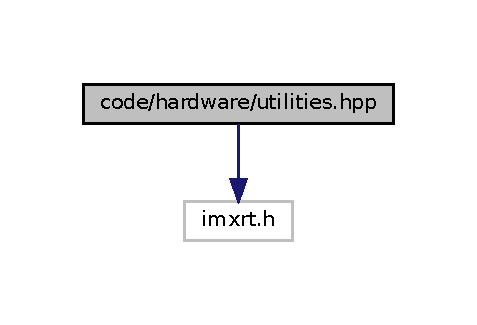
\includegraphics[width=229pt]{df/d46/utilities_8hpp__incl}
\end{center}
\end{figure}
This graph shows which files directly or indirectly include this file\+:
\nopagebreak
\begin{figure}[H]
\begin{center}
\leavevmode
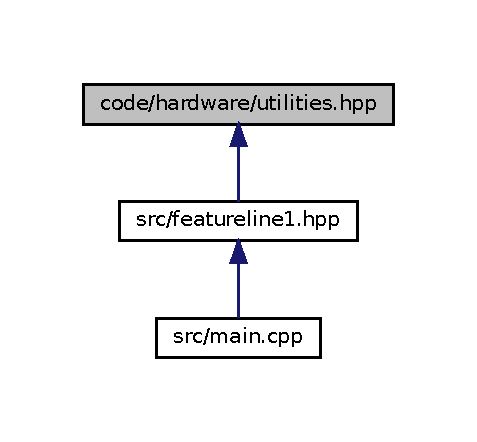
\includegraphics[width=229pt]{db/d84/utilities_8hpp__dep__incl}
\end{center}
\end{figure}
\subsection*{Macros}
\begin{DoxyCompactItemize}
\item 
\#define \hyperlink{utilities_8hpp_a4063879653b587261fa428e2a9d662b4}{P\+R\+R\+EG}(x)~Serial.\+print(\#x\char`\"{} 0x\char`\"{}); Serial.\+println(x,\+H\+E\+X)
\end{DoxyCompactItemize}
\subsection*{Functions}
\begin{DoxyCompactItemize}
\item 
void \hyperlink{utilities_8hpp_aceb15fdf783b1e9be1ef0d0fff5b5907}{xbar\+\_\+connect} (unsigned int input, unsigned int output)
\begin{DoxyCompactList}\small\item\em Establishes connection over X\+B\+A\+R1-\/A, given the input and output xbar pins  -\/ \href{https://github.com/manitou48/teensy4/blob/bc8fc46af5065a3f84352e0474069ae7a1a13064/pitxbaradc.ino#L40}{\tt https\+://github.\+com/manitou48/teensy4/blob/bc8fc46af5065a3f84352e0474069ae7a1a13064/pitxbaradc.\+ino\#\+L40}  -\/ Not specified. \end{DoxyCompactList}\item 
uint32\+\_\+t \hyperlink{utilities_8hpp_a1fb00a623d8b292185132f57935148a9}{F\+\_\+\+C\+P\+U\+\_\+tick\+\_\+count} ()
\item 
float \hyperlink{utilities_8hpp_a126c38ddf2ada96665a56b590a631776}{get\+\_\+\+C\+P\+U\+\_\+temp} ()
\end{DoxyCompactItemize}


\subsection{Macro Definition Documentation}
\mbox{\Hypertarget{utilities_8hpp_a4063879653b587261fa428e2a9d662b4}\label{utilities_8hpp_a4063879653b587261fa428e2a9d662b4}} 
\index{utilities.\+hpp@{utilities.\+hpp}!P\+R\+R\+EG@{P\+R\+R\+EG}}
\index{P\+R\+R\+EG@{P\+R\+R\+EG}!utilities.\+hpp@{utilities.\+hpp}}
\subsubsection{\texorpdfstring{P\+R\+R\+EG}{PRREG}}
{\footnotesize\ttfamily \#define P\+R\+R\+EG(\begin{DoxyParamCaption}\item[{}]{x }\end{DoxyParamCaption})~Serial.\+print(\#x\char`\"{} 0x\char`\"{}); Serial.\+println(x,\+H\+E\+X)}



\subsection{Function Documentation}
\mbox{\Hypertarget{utilities_8hpp_a1fb00a623d8b292185132f57935148a9}\label{utilities_8hpp_a1fb00a623d8b292185132f57935148a9}} 
\index{utilities.\+hpp@{utilities.\+hpp}!F\+\_\+\+C\+P\+U\+\_\+tick\+\_\+count@{F\+\_\+\+C\+P\+U\+\_\+tick\+\_\+count}}
\index{F\+\_\+\+C\+P\+U\+\_\+tick\+\_\+count@{F\+\_\+\+C\+P\+U\+\_\+tick\+\_\+count}!utilities.\+hpp@{utilities.\+hpp}}
\subsubsection{\texorpdfstring{F\+\_\+\+C\+P\+U\+\_\+tick\+\_\+count()}{F\_CPU\_tick\_count()}}
{\footnotesize\ttfamily uint32\+\_\+t F\+\_\+\+C\+P\+U\+\_\+tick\+\_\+count (\begin{DoxyParamCaption}{ }\end{DoxyParamCaption})}

\mbox{\Hypertarget{utilities_8hpp_a126c38ddf2ada96665a56b590a631776}\label{utilities_8hpp_a126c38ddf2ada96665a56b590a631776}} 
\index{utilities.\+hpp@{utilities.\+hpp}!get\+\_\+\+C\+P\+U\+\_\+temp@{get\+\_\+\+C\+P\+U\+\_\+temp}}
\index{get\+\_\+\+C\+P\+U\+\_\+temp@{get\+\_\+\+C\+P\+U\+\_\+temp}!utilities.\+hpp@{utilities.\+hpp}}
\subsubsection{\texorpdfstring{get\+\_\+\+C\+P\+U\+\_\+temp()}{get\_CPU\_temp()}}
{\footnotesize\ttfamily float get\+\_\+\+C\+P\+U\+\_\+temp (\begin{DoxyParamCaption}{ }\end{DoxyParamCaption})}

\mbox{\Hypertarget{utilities_8hpp_aceb15fdf783b1e9be1ef0d0fff5b5907}\label{utilities_8hpp_aceb15fdf783b1e9be1ef0d0fff5b5907}} 
\index{utilities.\+hpp@{utilities.\+hpp}!xbar\+\_\+connect@{xbar\+\_\+connect}}
\index{xbar\+\_\+connect@{xbar\+\_\+connect}!utilities.\+hpp@{utilities.\+hpp}}
\subsubsection{\texorpdfstring{xbar\+\_\+connect()}{xbar\_connect()}}
{\footnotesize\ttfamily void xbar\+\_\+connect (\begin{DoxyParamCaption}\item[{unsigned int}]{input,  }\item[{unsigned int}]{output }\end{DoxyParamCaption})}



Establishes connection over X\+B\+A\+R1-\/A, given the input and output xbar pins  -\/ \href{https://github.com/manitou48/teensy4/blob/bc8fc46af5065a3f84352e0474069ae7a1a13064/pitxbaradc.ino#L40}{\tt https\+://github.\+com/manitou48/teensy4/blob/bc8fc46af5065a3f84352e0474069ae7a1a13064/pitxbaradc.\+ino\#\+L40}  -\/ Not specified. 


\hypertarget{accumulator_8hpp}{}\section{lib/software/accumulator.hpp File Reference}
\label{accumulator_8hpp}\index{lib/software/accumulator.\+hpp@{lib/software/accumulator.\+hpp}}
{\ttfamily \#include \char`\"{}types.\+hpp\char`\"{}}\newline
{\ttfamily \#include \char`\"{}Lin\+\_\+\+A\+Corr\+\_\+\+R\+T\+\_\+\+Base.\+hpp\char`\"{}}\newline
Include dependency graph for accumulator.\+hpp\+:
\nopagebreak
\begin{figure}[H]
\begin{center}
\leavevmode
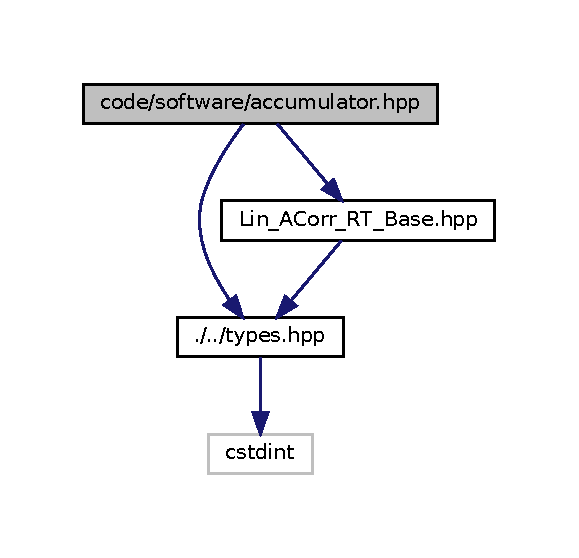
\includegraphics[width=272pt]{accumulator_8hpp__incl}
\end{center}
\end{figure}
This graph shows which files directly or indirectly include this file\+:
\nopagebreak
\begin{figure}[H]
\begin{center}
\leavevmode
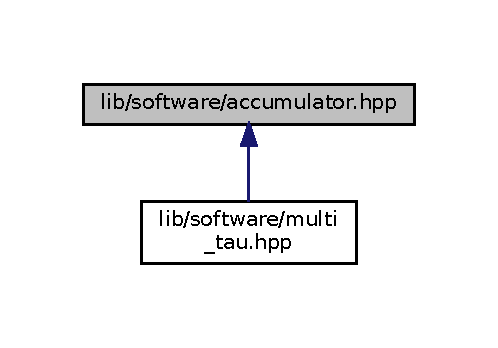
\includegraphics[width=239pt]{accumulator_8hpp__dep__incl}
\end{center}
\end{figure}
\subsection*{Classes}
\begin{DoxyCompactItemize}
\item 
class \hyperlink{classAccumulator}{Accumulator}
\begin{DoxyCompactList}\small\item\em Adapter object responsible for accumulating the points and coarsening the time-\/series as per the relavent linear-\/correlator time-\/resolution. \end{DoxyCompactList}\end{DoxyCompactItemize}

\hypertarget{circular__buffer_8hpp}{}\section{/mnt/m/code/\+Correlator/\+Software/circular\+\_\+buffer.hpp File Reference}
\label{circular__buffer_8hpp}\index{/mnt/m/code/\+Correlator/\+Software/circular\+\_\+buffer.\+hpp@{/mnt/m/code/\+Correlator/\+Software/circular\+\_\+buffer.\+hpp}}
\subsection*{Classes}
\begin{DoxyCompactItemize}
\item 
class \hyperlink{classCircular__Buffer}{Circular\+\_\+\+Buffer$<$ Type, Max\+Size $>$}
\begin{DoxyCompactList}\small\item\em Implementation of simple Serial Buffer with bounded index random accessor. \end{DoxyCompactList}\end{DoxyCompactItemize}

\hypertarget{discarder_8hpp}{}\section{/mnt/m/code/\+Correlator/\+Software/discarder.hpp File Reference}
\label{discarder_8hpp}\index{/mnt/m/code/\+Correlator/\+Software/discarder.\+hpp@{/mnt/m/code/\+Correlator/\+Software/discarder.\+hpp}}
{\ttfamily \#include \char`\"{}types.\+hpp\char`\"{}}\newline
{\ttfamily \#include \char`\"{}Lin\+\_\+\+A\+Corr\+\_\+\+R\+T\+\_\+\+Base.\+hpp\char`\"{}}\newline
Include dependency graph for discarder.\+hpp\+:
\nopagebreak
\begin{figure}[H]
\begin{center}
\leavevmode
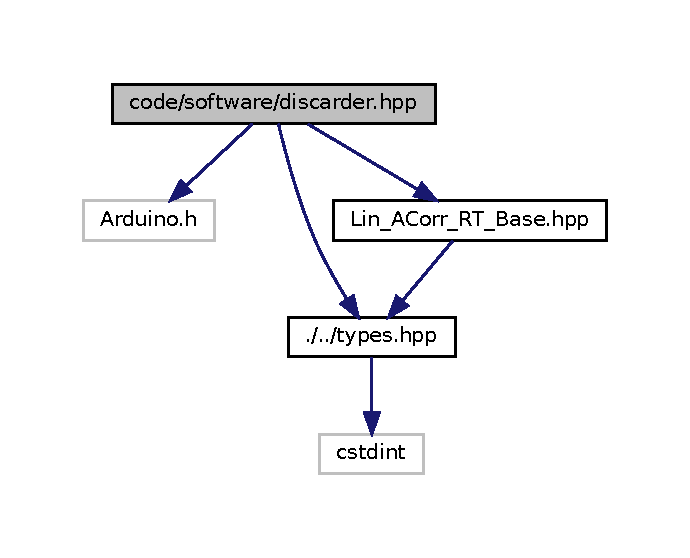
\includegraphics[width=259pt]{discarder_8hpp__incl}
\end{center}
\end{figure}
This graph shows which files directly or indirectly include this file\+:
\nopagebreak
\begin{figure}[H]
\begin{center}
\leavevmode
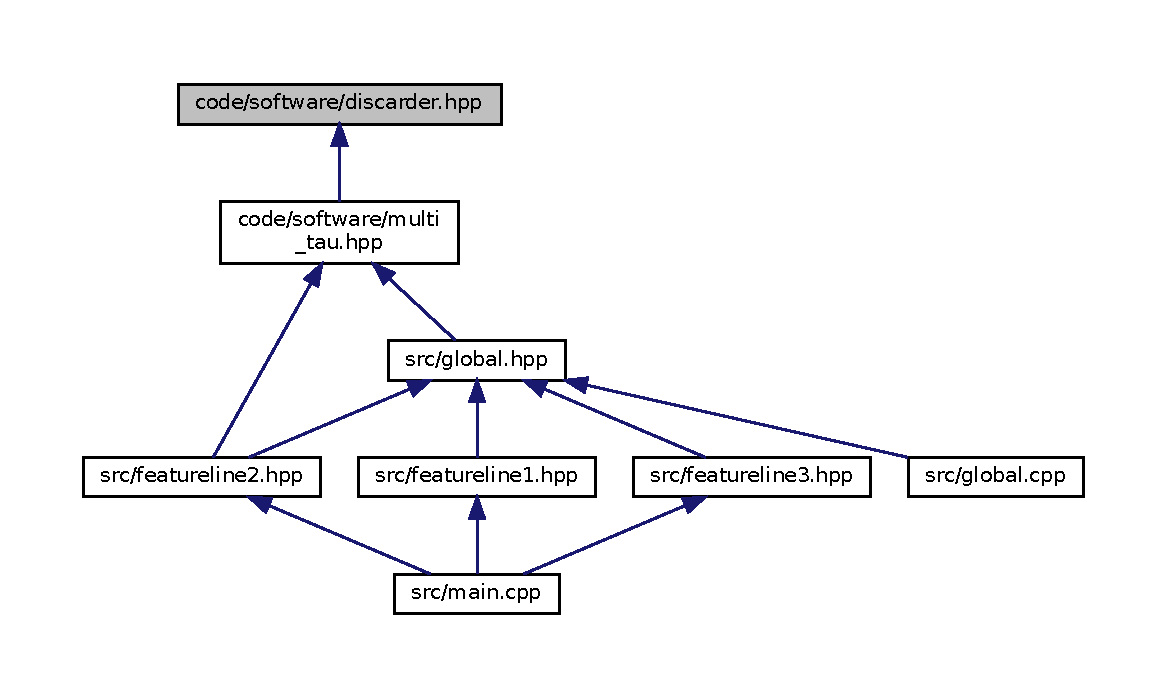
\includegraphics[width=214pt]{discarder_8hpp__dep__incl}
\end{center}
\end{figure}
\subsection*{Classes}
\begin{DoxyCompactItemize}
\item 
class \hyperlink{classFrontBack__Discarder__Base}{Front\+Back\+\_\+\+Discarder\+\_\+\+Base$<$ Series\+\_\+size, Front, End $>$}
\begin{DoxyCompactList}\small\item\em Base class for Front and Back discarder objects. \end{DoxyCompactList}\item 
class \hyperlink{classDiscarder__Teensy}{Discarder\+\_\+\+Teensy$<$ Series\+\_\+size, Front, End $>$}
\begin{DoxyCompactList}\small\item\em Teensy specific Front back discarder implementation. \end{DoxyCompactList}\end{DoxyCompactItemize}

\hypertarget{Lin__ACorr__RT__Base_8hpp}{}\section{code/software/\+Lin\+\_\+\+A\+Corr\+\_\+\+R\+T\+\_\+\+Base.hpp File Reference}
\label{Lin__ACorr__RT__Base_8hpp}\index{code/software/\+Lin\+\_\+\+A\+Corr\+\_\+\+R\+T\+\_\+\+Base.\+hpp@{code/software/\+Lin\+\_\+\+A\+Corr\+\_\+\+R\+T\+\_\+\+Base.\+hpp}}
{\ttfamily \#include \char`\"{}./../types.\+hpp\char`\"{}}\newline
Include dependency graph for Lin\+\_\+\+A\+Corr\+\_\+\+R\+T\+\_\+\+Base.\+hpp\+:
\nopagebreak
\begin{figure}[H]
\begin{center}
\leavevmode
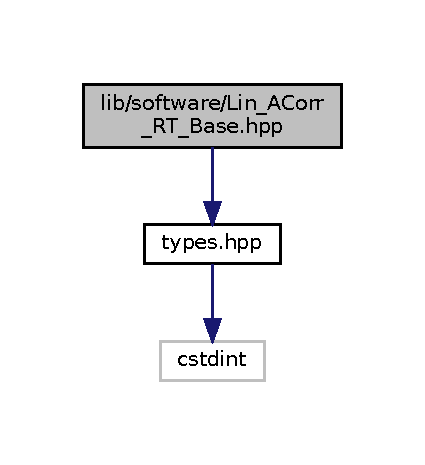
\includegraphics[width=215pt]{Lin__ACorr__RT__Base_8hpp__incl}
\end{center}
\end{figure}
This graph shows which files directly or indirectly include this file\+:
\nopagebreak
\begin{figure}[H]
\begin{center}
\leavevmode
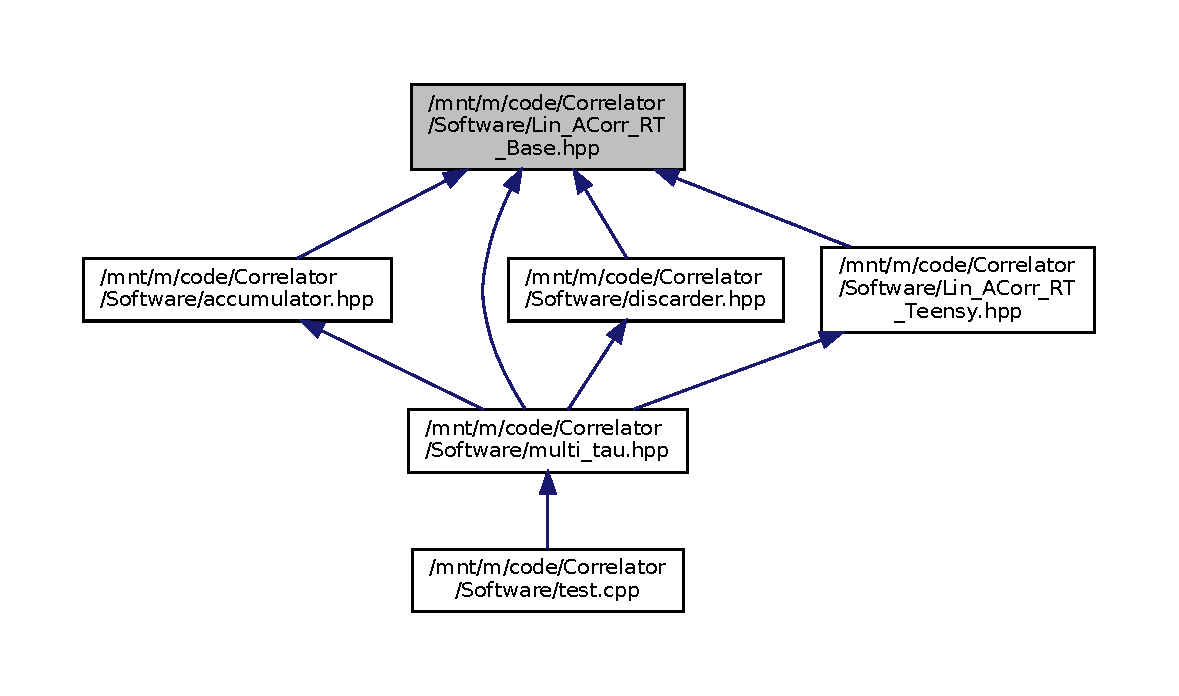
\includegraphics[width=350pt]{Lin__ACorr__RT__Base_8hpp__dep__incl}
\end{center}
\end{figure}
\subsection*{Classes}
\begin{DoxyCompactItemize}
\item 
class \hyperlink{classLin__ACorr__RT__Base}{Lin\+\_\+\+A\+Corr\+\_\+\+R\+T\+\_\+\+Base}
\begin{DoxyCompactList}\small\item\em This class is a blank interface for all objects that are — {\bfseries \{Linear} Real-\/\+Time Software Auto-\/\+Correlators\}. \end{DoxyCompactList}\end{DoxyCompactItemize}

\hypertarget{Lin__ACorr__RT__Teensy_8hpp}{}\section{code/software/\+Lin\+\_\+\+A\+Corr\+\_\+\+R\+T\+\_\+\+Teensy.hpp File Reference}
\label{Lin__ACorr__RT__Teensy_8hpp}\index{code/software/\+Lin\+\_\+\+A\+Corr\+\_\+\+R\+T\+\_\+\+Teensy.\+hpp@{code/software/\+Lin\+\_\+\+A\+Corr\+\_\+\+R\+T\+\_\+\+Teensy.\+hpp}}
{\ttfamily \#include \char`\"{}./../types.\+hpp\char`\"{}}\newline
{\ttfamily \#include \char`\"{}simpler\+\_\+circular\+\_\+buffer.\+hpp\char`\"{}}\newline
{\ttfamily \#include $<$Arduino.\+h$>$}\newline
Include dependency graph for Lin\+\_\+\+A\+Corr\+\_\+\+R\+T\+\_\+\+Teensy.\+hpp\+:
\nopagebreak
\begin{figure}[H]
\begin{center}
\leavevmode
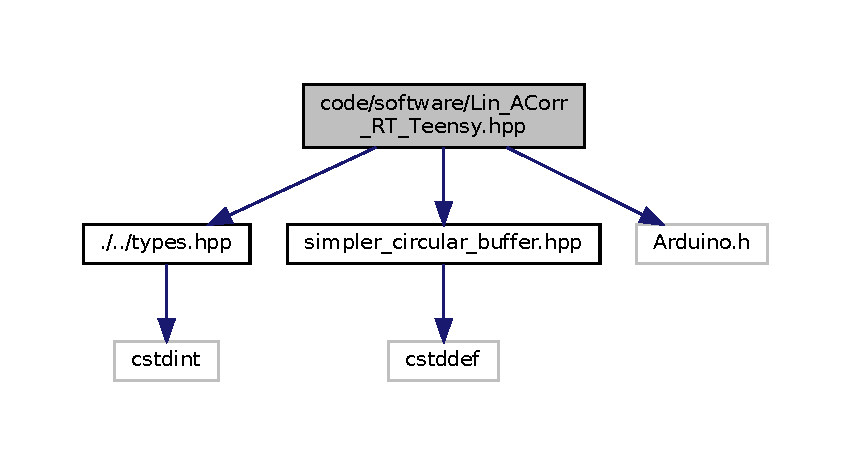
\includegraphics[width=350pt]{d5/d93/Lin__ACorr__RT__Teensy_8hpp__incl}
\end{center}
\end{figure}
This graph shows which files directly or indirectly include this file\+:
\nopagebreak
\begin{figure}[H]
\begin{center}
\leavevmode
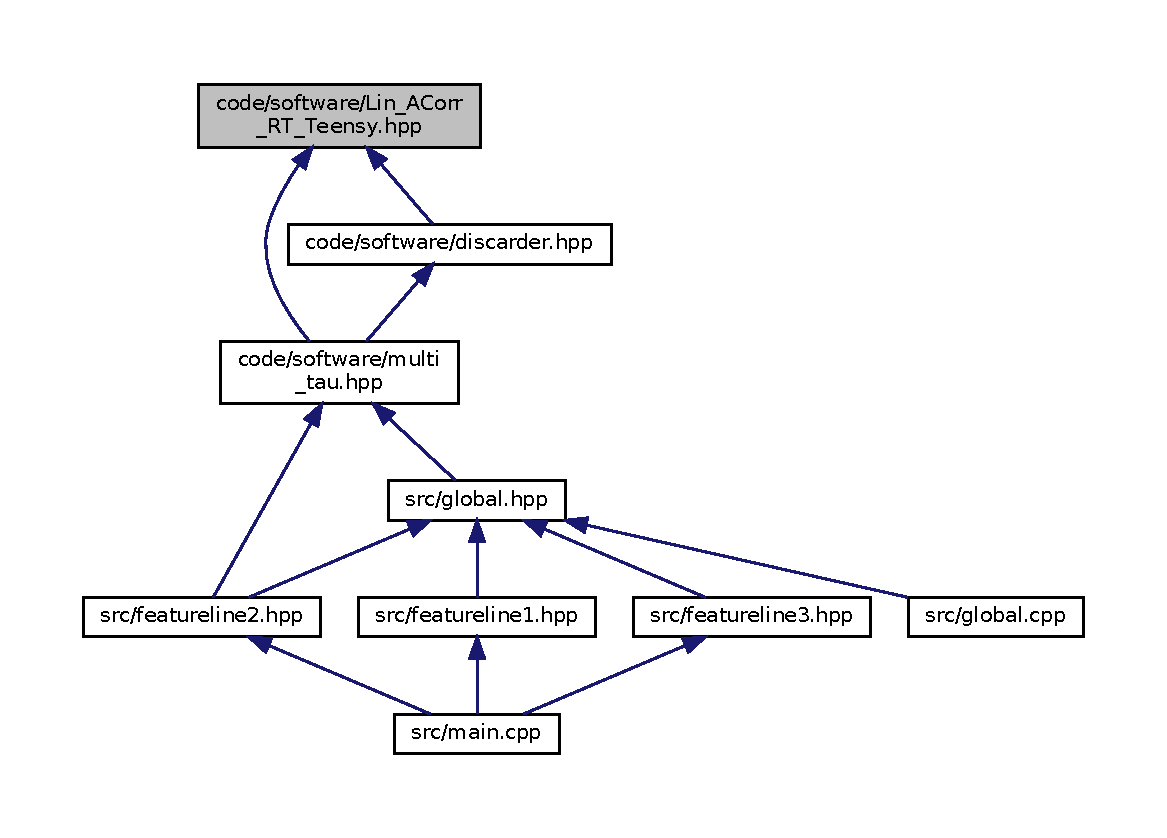
\includegraphics[width=350pt]{db/d9e/Lin__ACorr__RT__Teensy_8hpp__dep__incl}
\end{center}
\end{figure}
\subsection*{Classes}
\begin{DoxyCompactItemize}
\item 
class \hyperlink{classLinACorrRTTeensy}{Lin\+A\+Corr\+R\+T\+Teensy$<$ Series\+\_\+\+Size, has\+Monitor\+Channel $>$}
\begin{DoxyCompactList}\small\item\em This is an implementation of Lin\+\_\+\+A\+Corr\+\_\+\+R\+T\+\_\+\+Base for Teensy with {\bfseries }(No normalisation or baseline subtraction.) \end{DoxyCompactList}\end{DoxyCompactItemize}

\hypertarget{Lin__CrossCorr__RT__Base_8hpp}{}\section{/mnt/m/code/\+Correlator/\+Software/\+Lin\+\_\+\+Cross\+Corr\+\_\+\+R\+T\+\_\+\+Base.hpp File Reference}
\label{Lin__CrossCorr__RT__Base_8hpp}\index{/mnt/m/code/\+Correlator/\+Software/\+Lin\+\_\+\+Cross\+Corr\+\_\+\+R\+T\+\_\+\+Base.\+hpp@{/mnt/m/code/\+Correlator/\+Software/\+Lin\+\_\+\+Cross\+Corr\+\_\+\+R\+T\+\_\+\+Base.\+hpp}}
{\ttfamily \#include \char`\"{}types.\+hpp\char`\"{}}\newline
Include dependency graph for Lin\+\_\+\+Cross\+Corr\+\_\+\+R\+T\+\_\+\+Base.\+hpp\+:\nopagebreak
\begin{figure}[H]
\begin{center}
\leavevmode
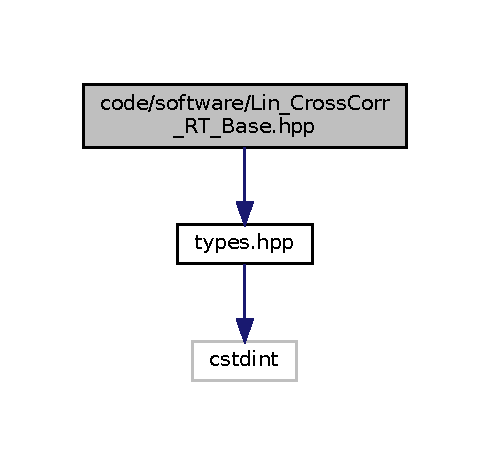
\includegraphics[width=213pt]{Lin__CrossCorr__RT__Base_8hpp__incl}
\end{center}
\end{figure}
This graph shows which files directly or indirectly include this file\+:\nopagebreak
\begin{figure}[H]
\begin{center}
\leavevmode
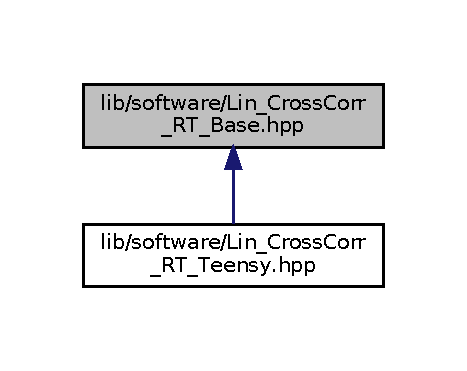
\includegraphics[width=213pt]{Lin__CrossCorr__RT__Base_8hpp__dep__incl}
\end{center}
\end{figure}
\subsection*{Classes}
\begin{DoxyCompactItemize}
\item 
class \hyperlink{classLin__CrossCorr__RT__Base}{Lin\+\_\+\+Cross\+Corr\+\_\+\+R\+T\+\_\+\+Base}
\begin{DoxyCompactList}\small\item\em This class is a blank interface for all objects that are — {\bfseries \{Linear} Real-\/\+Time Software Auto-\/\+Correlators\}. \end{DoxyCompactList}\end{DoxyCompactItemize}

\hypertarget{Lin__CrossCorr__RT__Teensy_8hpp}{}\section{code/software/\+Lin\+\_\+\+Cross\+Corr\+\_\+\+R\+T\+\_\+\+Teensy.hpp File Reference}
\label{Lin__CrossCorr__RT__Teensy_8hpp}\index{code/software/\+Lin\+\_\+\+Cross\+Corr\+\_\+\+R\+T\+\_\+\+Teensy.\+hpp@{code/software/\+Lin\+\_\+\+Cross\+Corr\+\_\+\+R\+T\+\_\+\+Teensy.\+hpp}}
{\ttfamily \#include \char`\"{}types.\+hpp\char`\"{}}\newline
{\ttfamily \#include \char`\"{}Lin\+\_\+\+Cross\+Corr\+\_\+\+R\+T\+\_\+\+Base.\+hpp\char`\"{}}\newline
Include dependency graph for Lin\+\_\+\+Cross\+Corr\+\_\+\+R\+T\+\_\+\+Teensy.\+hpp\+:
\nopagebreak
\begin{figure}[H]
\begin{center}
\leavevmode
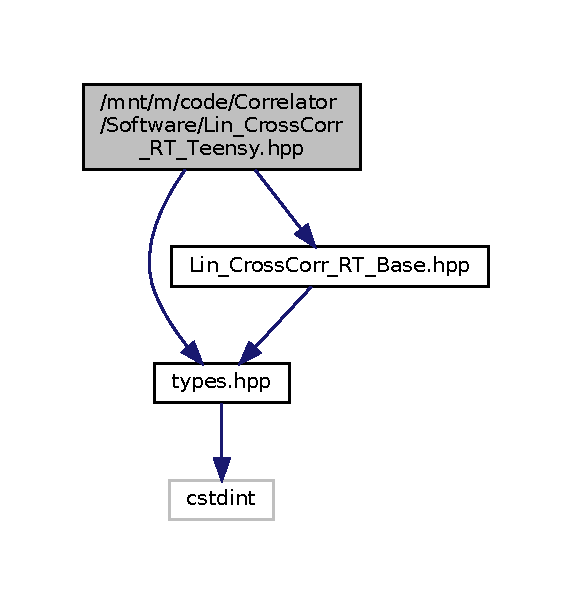
\includegraphics[width=286pt]{Lin__CrossCorr__RT__Teensy_8hpp__incl}
\end{center}
\end{figure}
\subsection*{Classes}
\begin{DoxyCompactItemize}
\item 
class \hyperlink{classLin__CrossCorr__RT__Teensy}{Lin\+\_\+\+Cross\+Corr\+\_\+\+R\+T\+\_\+\+Teensy$<$ Series\+\_\+size $>$}
\begin{DoxyCompactList}\small\item\em This is an implementation of \hyperlink{classLin__ACorr__RT__Base}{Lin\+\_\+\+A\+Corr\+\_\+\+R\+T\+\_\+\+Base} for Teensy with {\bfseries }(No normalisation or baseline subtraction.) \end{DoxyCompactList}\end{DoxyCompactItemize}

\hypertarget{multi__tau_8hpp}{}\section{code/software/multi\+\_\+tau.hpp File Reference}
\label{multi__tau_8hpp}\index{code/software/multi\+\_\+tau.\+hpp@{code/software/multi\+\_\+tau.\+hpp}}
{\ttfamily \#include $<$cmath$>$}\newline
{\ttfamily \#include \char`\"{}./../types.\+hpp\char`\"{}}\newline
{\ttfamily \#include \char`\"{}Lin\+\_\+\+A\+Corr\+\_\+\+R\+T\+\_\+\+Teensy.\+hpp\char`\"{}}\newline
{\ttfamily \#include \char`\"{}accumulator.\+hpp\char`\"{}}\newline
{\ttfamily \#include \char`\"{}discarder.\+hpp\char`\"{}}\newline
{\ttfamily \#include \char`\"{}monitor\+\_\+channel.\+hpp\char`\"{}}\newline
Include dependency graph for multi\+\_\+tau.\+hpp\+:
\nopagebreak
\begin{figure}[H]
\begin{center}
\leavevmode
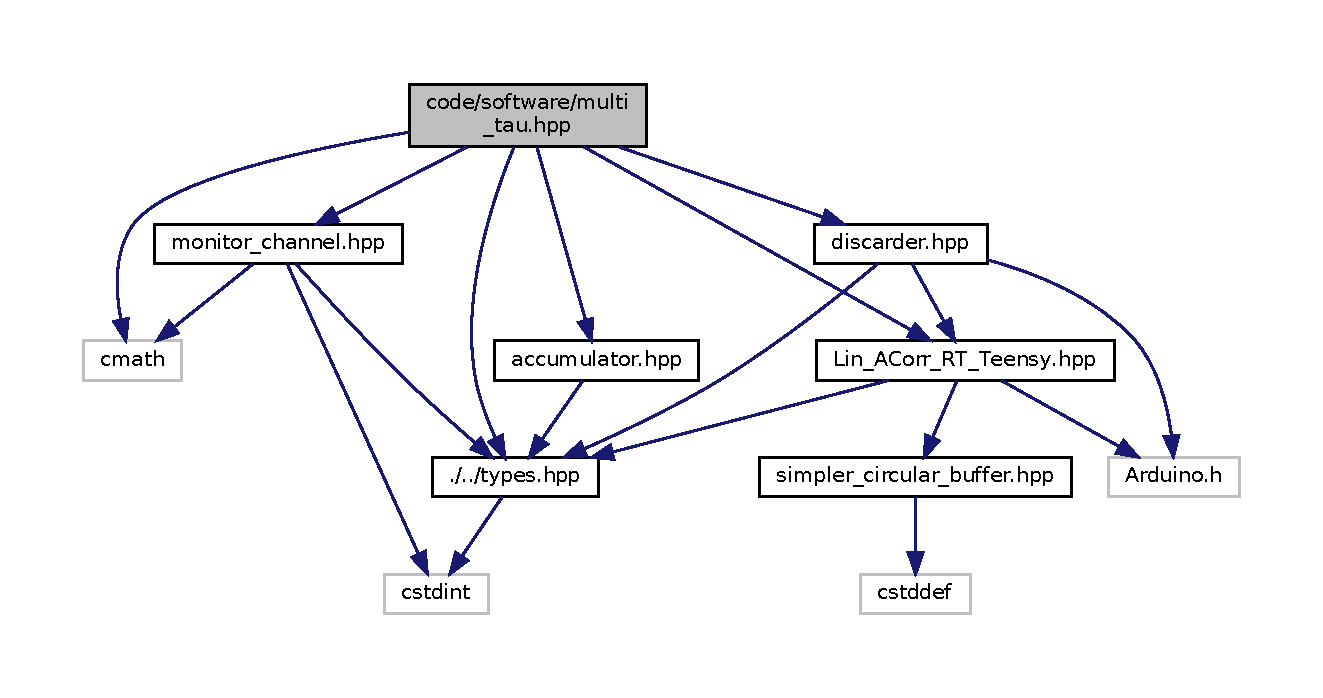
\includegraphics[width=350pt]{de/df4/multi__tau_8hpp__incl}
\end{center}
\end{figure}
This graph shows which files directly or indirectly include this file\+:
\nopagebreak
\begin{figure}[H]
\begin{center}
\leavevmode
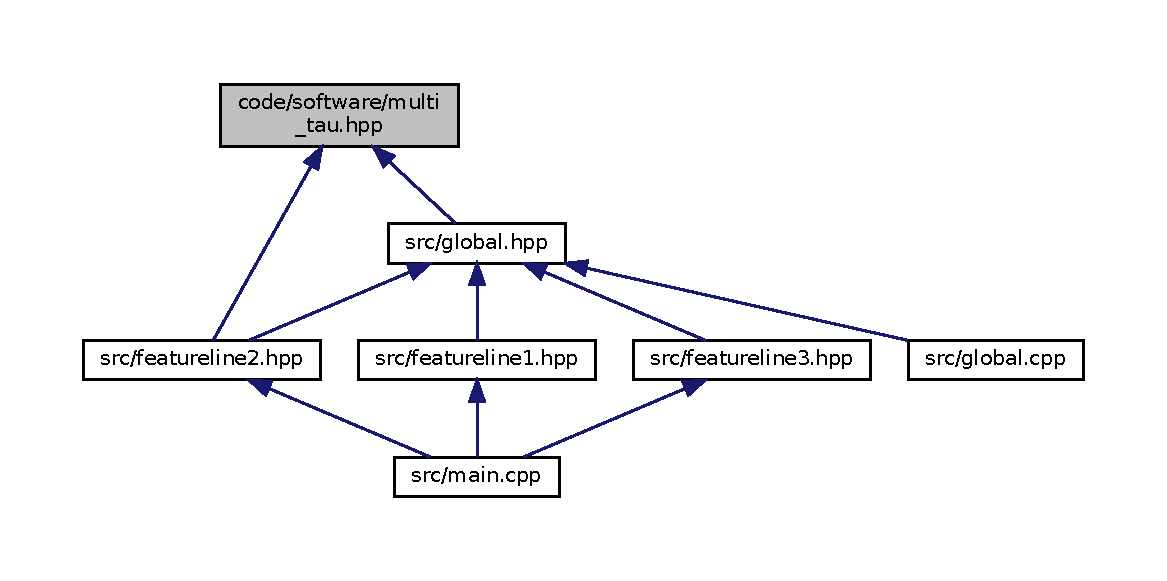
\includegraphics[width=350pt]{d3/d49/multi__tau_8hpp__dep__incl}
\end{center}
\end{figure}
\subsection*{Classes}
\begin{DoxyCompactItemize}
\item 
class \hyperlink{classMultiTauACorrRTTeensy}{Multi\+Tau\+A\+Corr\+R\+T\+Teensy$<$ Lin\+\_\+channels, Series\+\_\+size, Bin\+\_\+\+Ratio $>$}
\begin{DoxyCompactList}\small\item\em Multi\+Tau Auto-\/\+Correlator object that is composed of multiple linear -\/ autocorrelators. Specialised for teensy. \end{DoxyCompactList}\end{DoxyCompactItemize}

\hypertarget{simpler__circular__buffer_8hpp}{}\section{lib/software/simpler\+\_\+circular\+\_\+buffer.hpp File Reference}
\label{simpler__circular__buffer_8hpp}\index{lib/software/simpler\+\_\+circular\+\_\+buffer.\+hpp@{lib/software/simpler\+\_\+circular\+\_\+buffer.\+hpp}}
{\ttfamily \#include $<$cstddef$>$}\newline
Include dependency graph for simpler\+\_\+circular\+\_\+buffer.\+hpp\+:
\nopagebreak
\begin{figure}[H]
\begin{center}
\leavevmode
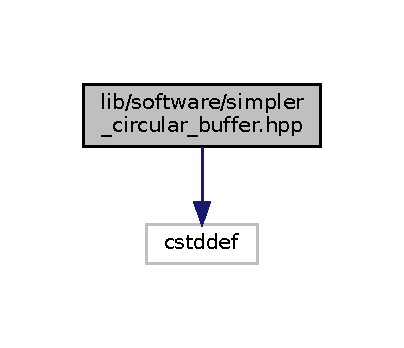
\includegraphics[width=194pt]{simpler__circular__buffer_8hpp__incl}
\end{center}
\end{figure}
\subsection*{Classes}
\begin{DoxyCompactItemize}
\item 
class \hyperlink{classSimpler__Circular__Buffer}{Simpler\+\_\+\+Circular\+\_\+\+Buffer$<$ Type, Max\+Size $>$}
\end{DoxyCompactItemize}

\hypertarget{types_8hpp}{}\section{code/types.hpp File Reference}
\label{types_8hpp}\index{code/types.\+hpp@{code/types.\+hpp}}
{\ttfamily \#include $<$cstdint$>$}\newline
Include dependency graph for types.\+hpp\+:\nopagebreak
\begin{figure}[H]
\begin{center}
\leavevmode
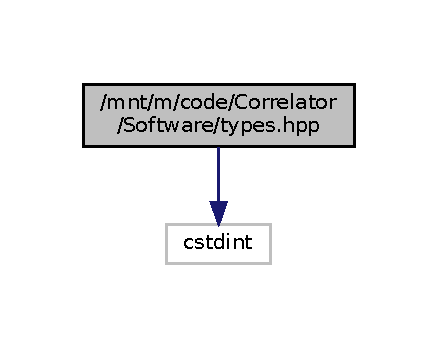
\includegraphics[width=171pt]{types_8hpp__incl}
\end{center}
\end{figure}
This graph shows which files directly or indirectly include this file\+:
\nopagebreak
\begin{figure}[H]
\begin{center}
\leavevmode
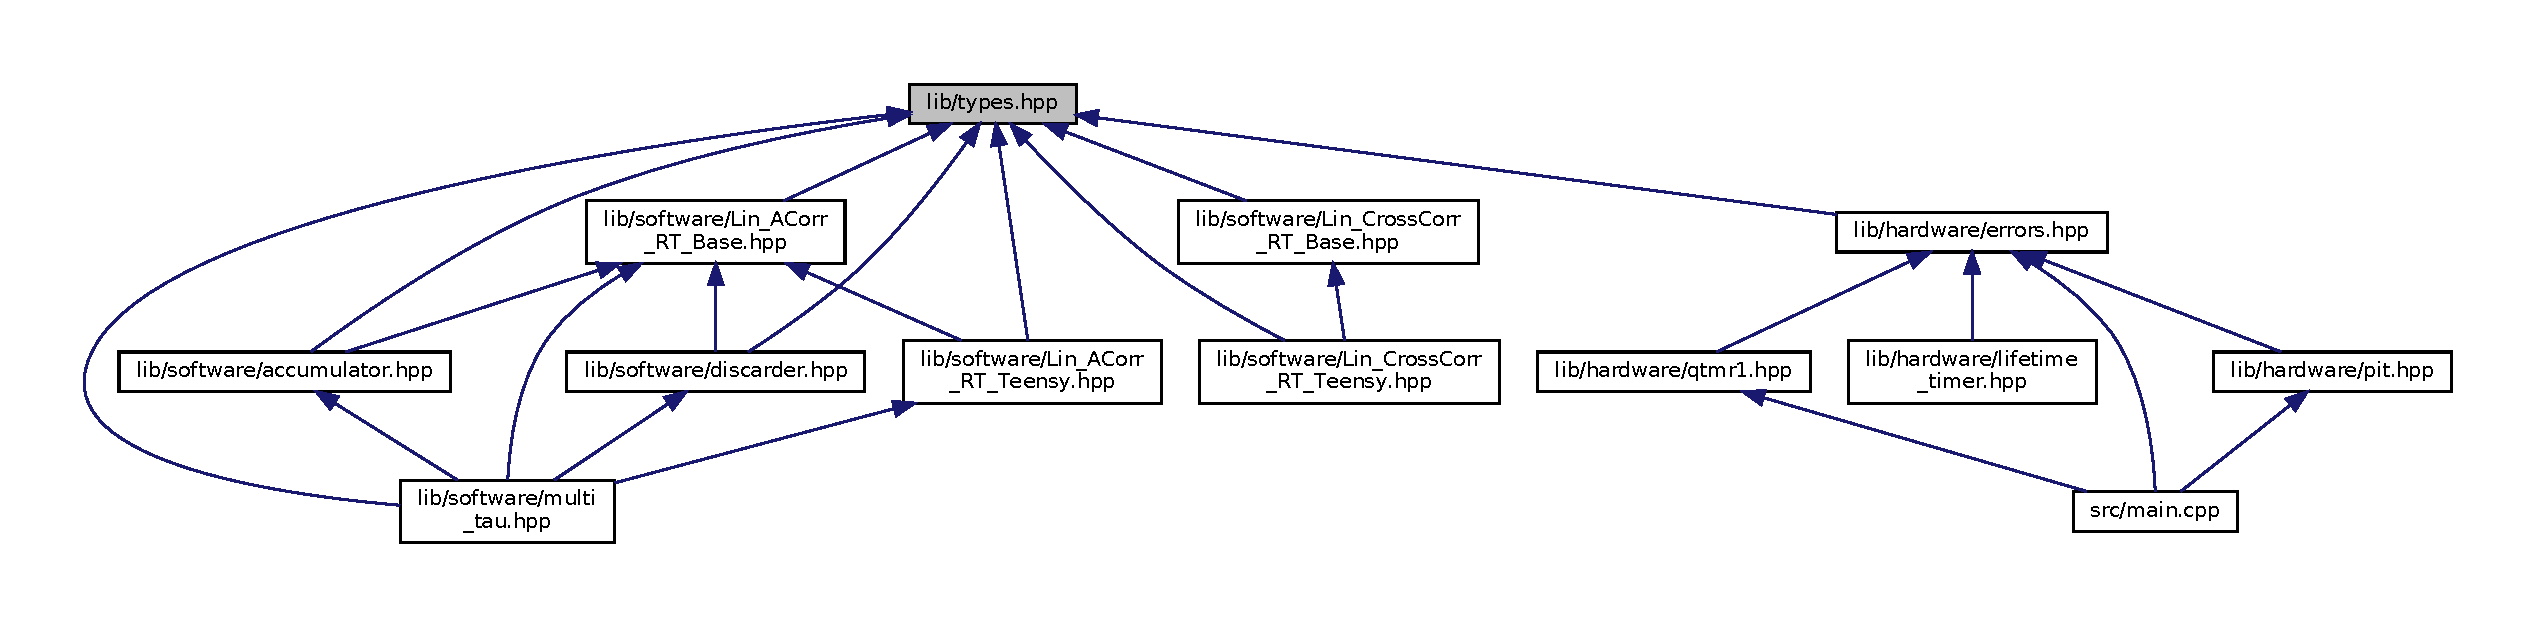
\includegraphics[width=350pt]{types_8hpp__dep__incl}
\end{center}
\end{figure}
\subsection*{Typedefs}
\begin{DoxyCompactItemize}
\item 
using \hyperlink{types_8hpp_a22f279793847eba127de149437848c48}{counter\+\_\+t} = uint32\+\_\+t
\begin{DoxyCompactList}\small\item\em Data type received from the pulse counter. It is the fundamental type used for representing series data. \end{DoxyCompactList}\item 
using \hyperlink{types_8hpp_a7c40bb931c31595ed6308605f4537447}{index\+\_\+t} = uint\+\_\+fast8\+\_\+t
\begin{DoxyCompactList}\small\item\em It is used as the array indices and thus determine the maximum size of the Channel\+\_\+array and the Series\+\_\+array. \end{DoxyCompactList}\end{DoxyCompactItemize}


\subsection{Typedef Documentation}
\mbox{\Hypertarget{types_8hpp_a22f279793847eba127de149437848c48}\label{types_8hpp_a22f279793847eba127de149437848c48}} 
\index{types.\+hpp@{types.\+hpp}!counter\+\_\+t@{counter\+\_\+t}}
\index{counter\+\_\+t@{counter\+\_\+t}!types.\+hpp@{types.\+hpp}}
\subsubsection{\texorpdfstring{counter\+\_\+t}{counter\_t}}
{\footnotesize\ttfamily using \hyperlink{types_8hpp_a22f279793847eba127de149437848c48}{counter\+\_\+t} =  uint32\+\_\+t}



Data type received from the pulse counter. It is the fundamental type used for representing series data. 

\mbox{\Hypertarget{types_8hpp_a7c40bb931c31595ed6308605f4537447}\label{types_8hpp_a7c40bb931c31595ed6308605f4537447}} 
\index{types.\+hpp@{types.\+hpp}!index\+\_\+t@{index\+\_\+t}}
\index{index\+\_\+t@{index\+\_\+t}!types.\+hpp@{types.\+hpp}}
\subsubsection{\texorpdfstring{index\+\_\+t}{index\_t}}
{\footnotesize\ttfamily using \hyperlink{types_8hpp_a7c40bb931c31595ed6308605f4537447}{index\+\_\+t} =  uint\+\_\+fast8\+\_\+t}



It is used as the array indices and thus determine the maximum size of the Channel\+\_\+array and the Series\+\_\+array. 


\hypertarget{README_8md}{}\section{R\+E\+A\+D\+M\+E.\+md File Reference}
\label{README_8md}\index{R\+E\+A\+D\+M\+E.\+md@{R\+E\+A\+D\+M\+E.\+md}}

\hypertarget{code_2software_2README_8md}{}\section{code/software/\+R\+E\+A\+D\+ME.md File Reference}
\label{code_2software_2README_8md}\index{code/software/\+R\+E\+A\+D\+M\+E.\+md@{code/software/\+R\+E\+A\+D\+M\+E.\+md}}

\hypertarget{code_2hardware_2README_8md}{}\section{code/hardware/\+R\+E\+A\+D\+ME.md File Reference}
\label{code_2hardware_2README_8md}\index{code/hardware/\+R\+E\+A\+D\+M\+E.\+md@{code/hardware/\+R\+E\+A\+D\+M\+E.\+md}}

\hypertarget{main_8cpp}{}\section{src/main.cpp File Reference}
\label{main_8cpp}\index{src/main.\+cpp@{src/main.\+cpp}}
{\ttfamily \#include $<$Arduino.\+h$>$}\newline
{\ttfamily \#include $<$imxrt.\+h$>$}\newline
{\ttfamily \#include $<$hardware/pins.\+hpp$>$}\newline
{\ttfamily \#include $<$hardware/errors.\+hpp$>$}\newline
{\ttfamily \#include $<$hardware/pit.\+hpp$>$}\newline
{\ttfamily \#include $<$hardware/qtmr1.\+hpp$>$}\newline
{\ttfamily \#include $<$hardware/ledset.\+hpp$>$}\newline
{\ttfamily \#include $<$hardware/utilities.\+hpp$>$}\newline
{\ttfamily \#include $<$software/multi\+\_\+tau$>$}\newline
{\ttfamily \#include $<$hardware.\+hpp$>$}\newline
Include dependency graph for main.\+cpp\+:
\nopagebreak
\begin{figure}[H]
\begin{center}
\leavevmode
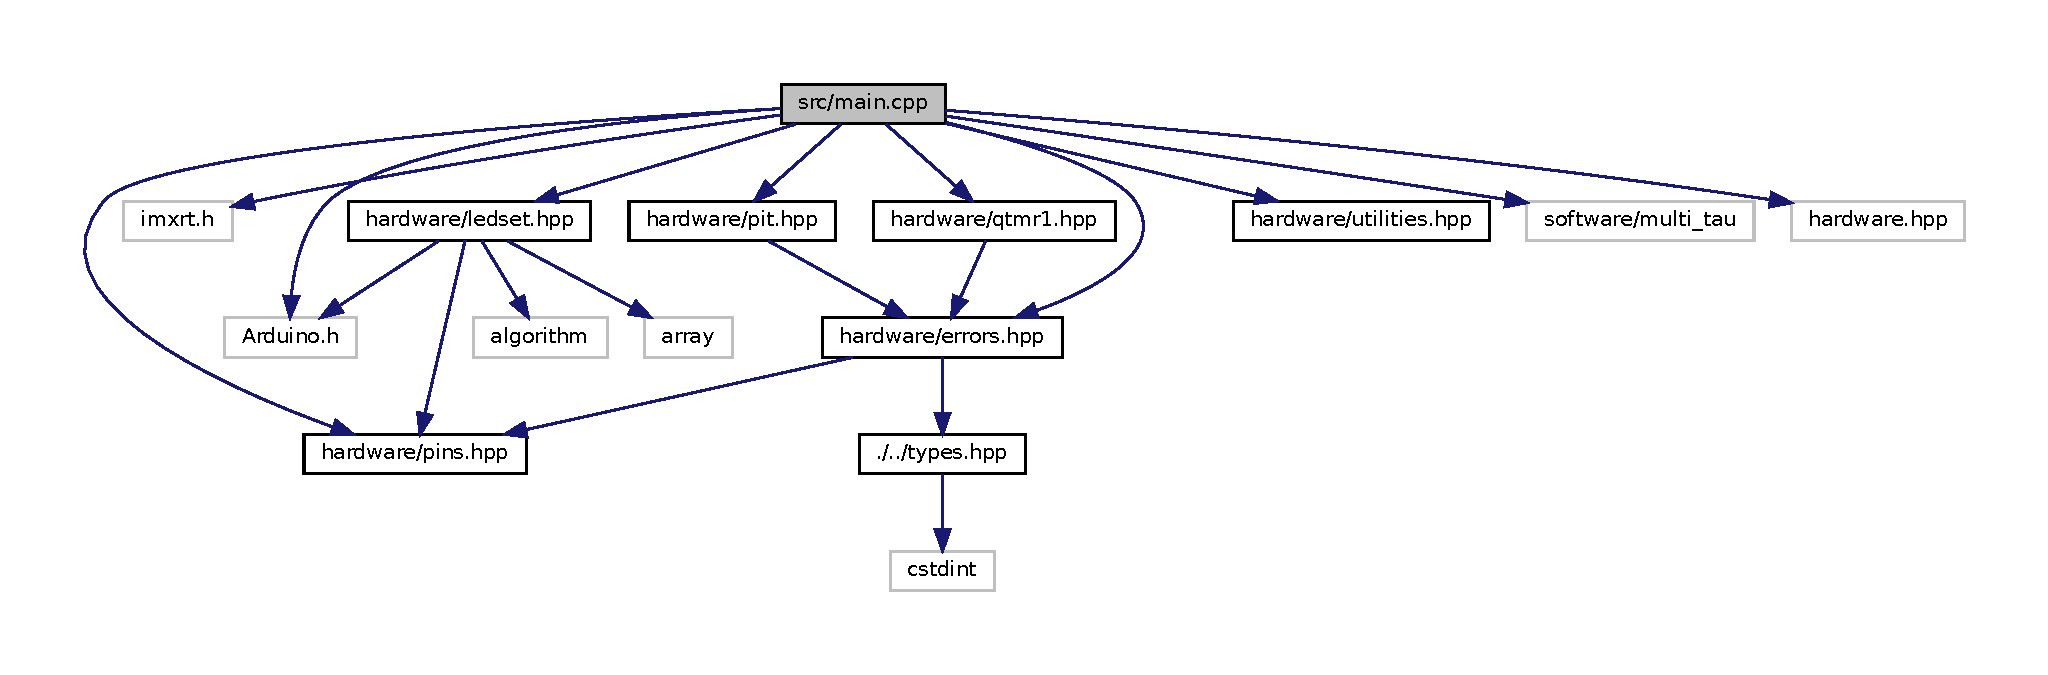
\includegraphics[width=350pt]{main_8cpp__incl}
\end{center}
\end{figure}
\subsection*{Macros}
\begin{DoxyCompactItemize}
\item 
\#define \hyperlink{main_8cpp_adcc5d50bb7482faf811186cd946b4a7d}{P\+I\+T\+\_\+\+T\+O\+G\+G\+L\+E\+\_\+\+T\+E\+S\+T\+\_\+\+P\+IN}~4
\begin{DoxyCompactList}\small\item\em L\+ED Dashboard resources. \end{DoxyCompactList}\end{DoxyCompactItemize}
\subsection*{Functions}
\begin{DoxyCompactItemize}
\item 
void \hyperlink{main_8cpp_a4fc01d736fe50cf5b977f755b675f11d}{setup} ()
\item 
void \hyperlink{main_8cpp_afe461d27b9c48d5921c00d521181f12f}{loop} ()
\item 
void \hyperlink{main_8cpp_a4d7b9fc4c1fccb2b242ac7e5f2d51fb7}{pit\+\_\+isr} ()
\end{DoxyCompactItemize}
\subsection*{Variables}
\begin{DoxyCompactItemize}
\item 
\hyperlink{classPITController}{P\+I\+T\+Controller}$<$ 2 $>$ \hyperlink{main_8cpp_a30d4468a263e3498d6e00f5b8eb99275}{P\+I\+\_\+t}
\begin{DoxyCompactList}\small\item\em P\+I\+\_\+t Resource. \end{DoxyCompactList}\item 
\hyperlink{classTMR1Controller}{T\+M\+R1\+Controller} \hyperlink{main_8cpp_a691981c43e1bdddca6df5accb6927331}{T\+T\+L\+\_\+c}
\begin{DoxyCompactList}\small\item\em T\+T\+L\+\_\+c Resource. \end{DoxyCompactList}\item 
\hyperlink{classLEDSet}{L\+E\+D\+Set} \hyperlink{main_8cpp_a40da5321d72e5a142e0c9719c8f9090a}{L\+E\+Dset}
\item 
volatile \hyperlink{types_8hpp_ac89ac912f524b3e3fa3720ea55fec966}{counter\+\_\+t} \hyperlink{main_8cpp_afcac7adcea259024440f8d9257d82d08}{Counter\+\_\+val} = 0
\begin{DoxyCompactList}\small\item\em Stores the value read by the counter. \end{DoxyCompactList}\item 
volatile bool \hyperlink{main_8cpp_afaf7617e9ce0486d54a6c65fedeaf1f9}{Update\+\_\+flag} = false
\begin{DoxyCompactList}\small\item\em Indicates if a new value has arrived from the counting module. \end{DoxyCompactList}\item 
volatile unsigned int \hyperlink{main_8cpp_aec1fbfd9bfc90e447b39a9362a0c51de}{Update\+\_\+count} = 0
\begin{DoxyCompactList}\small\item\em Stores the number of updates made on the correlator channels. \end{DoxyCompactList}\item 
const unsigned int \hyperlink{main_8cpp_a3b247283a68292408b626904e422a52e}{Serial\+Out\+\_\+\+Count\+Max} = 1
\begin{DoxyCompactList}\small\item\em Serial output is done after these many updates. \end{DoxyCompactList}\item 
const double \hyperlink{main_8cpp_a1d18182f432f5b88cf58be9c367be457}{Gate\+\_\+time\+\_\+us} = 1
\begin{DoxyCompactList}\small\item\em The gate time of T\+T\+L\+\_\+C in microseconds (us) \end{DoxyCompactList}\item 
const double \hyperlink{main_8cpp_ada17f1639ca8a5932f17942031baa67f}{Allowed\+\_\+period\+\_\+error\+\_\+us} = 1e-\/3
\begin{DoxyCompactList}\small\item\em Gate time precision error due to finite precision of timers. \end{DoxyCompactList}\end{DoxyCompactItemize}


\subsection{Macro Definition Documentation}
\mbox{\Hypertarget{main_8cpp_adcc5d50bb7482faf811186cd946b4a7d}\label{main_8cpp_adcc5d50bb7482faf811186cd946b4a7d}} 
\index{main.\+cpp@{main.\+cpp}!P\+I\+T\+\_\+\+T\+O\+G\+G\+L\+E\+\_\+\+T\+E\+S\+T\+\_\+\+P\+IN@{P\+I\+T\+\_\+\+T\+O\+G\+G\+L\+E\+\_\+\+T\+E\+S\+T\+\_\+\+P\+IN}}
\index{P\+I\+T\+\_\+\+T\+O\+G\+G\+L\+E\+\_\+\+T\+E\+S\+T\+\_\+\+P\+IN@{P\+I\+T\+\_\+\+T\+O\+G\+G\+L\+E\+\_\+\+T\+E\+S\+T\+\_\+\+P\+IN}!main.\+cpp@{main.\+cpp}}
\subsubsection{\texorpdfstring{P\+I\+T\+\_\+\+T\+O\+G\+G\+L\+E\+\_\+\+T\+E\+S\+T\+\_\+\+P\+IN}{PIT\_TOGGLE\_TEST\_PIN}}
{\footnotesize\ttfamily \#define P\+I\+T\+\_\+\+T\+O\+G\+G\+L\+E\+\_\+\+T\+E\+S\+T\+\_\+\+P\+IN~4}



L\+ED Dashboard resources. 



\subsection{Function Documentation}
\mbox{\Hypertarget{main_8cpp_afe461d27b9c48d5921c00d521181f12f}\label{main_8cpp_afe461d27b9c48d5921c00d521181f12f}} 
\index{main.\+cpp@{main.\+cpp}!loop@{loop}}
\index{loop@{loop}!main.\+cpp@{main.\+cpp}}
\subsubsection{\texorpdfstring{loop()}{loop()}}
{\footnotesize\ttfamily void loop (\begin{DoxyParamCaption}{ }\end{DoxyParamCaption})}

\mbox{\Hypertarget{main_8cpp_a4d7b9fc4c1fccb2b242ac7e5f2d51fb7}\label{main_8cpp_a4d7b9fc4c1fccb2b242ac7e5f2d51fb7}} 
\index{main.\+cpp@{main.\+cpp}!pit\+\_\+isr@{pit\+\_\+isr}}
\index{pit\+\_\+isr@{pit\+\_\+isr}!main.\+cpp@{main.\+cpp}}
\subsubsection{\texorpdfstring{pit\+\_\+isr()}{pit\_isr()}}
{\footnotesize\ttfamily void pit\+\_\+isr (\begin{DoxyParamCaption}{ }\end{DoxyParamCaption})}

\mbox{\Hypertarget{main_8cpp_a4fc01d736fe50cf5b977f755b675f11d}\label{main_8cpp_a4fc01d736fe50cf5b977f755b675f11d}} 
\index{main.\+cpp@{main.\+cpp}!setup@{setup}}
\index{setup@{setup}!main.\+cpp@{main.\+cpp}}
\subsubsection{\texorpdfstring{setup()}{setup()}}
{\footnotesize\ttfamily void setup (\begin{DoxyParamCaption}{ }\end{DoxyParamCaption})}



\subsection{Variable Documentation}
\mbox{\Hypertarget{main_8cpp_ada17f1639ca8a5932f17942031baa67f}\label{main_8cpp_ada17f1639ca8a5932f17942031baa67f}} 
\index{main.\+cpp@{main.\+cpp}!Allowed\+\_\+period\+\_\+error\+\_\+us@{Allowed\+\_\+period\+\_\+error\+\_\+us}}
\index{Allowed\+\_\+period\+\_\+error\+\_\+us@{Allowed\+\_\+period\+\_\+error\+\_\+us}!main.\+cpp@{main.\+cpp}}
\subsubsection{\texorpdfstring{Allowed\+\_\+period\+\_\+error\+\_\+us}{Allowed\_period\_error\_us}}
{\footnotesize\ttfamily const double Allowed\+\_\+period\+\_\+error\+\_\+us = 1e-\/3}



Gate time precision error due to finite precision of timers. 

\mbox{\Hypertarget{main_8cpp_afcac7adcea259024440f8d9257d82d08}\label{main_8cpp_afcac7adcea259024440f8d9257d82d08}} 
\index{main.\+cpp@{main.\+cpp}!Counter\+\_\+val@{Counter\+\_\+val}}
\index{Counter\+\_\+val@{Counter\+\_\+val}!main.\+cpp@{main.\+cpp}}
\subsubsection{\texorpdfstring{Counter\+\_\+val}{Counter\_val}}
{\footnotesize\ttfamily volatile \hyperlink{types_8hpp_ac89ac912f524b3e3fa3720ea55fec966}{counter\+\_\+t} Counter\+\_\+val = 0}



Stores the value read by the counter. 

\mbox{\Hypertarget{main_8cpp_a1d18182f432f5b88cf58be9c367be457}\label{main_8cpp_a1d18182f432f5b88cf58be9c367be457}} 
\index{main.\+cpp@{main.\+cpp}!Gate\+\_\+time\+\_\+us@{Gate\+\_\+time\+\_\+us}}
\index{Gate\+\_\+time\+\_\+us@{Gate\+\_\+time\+\_\+us}!main.\+cpp@{main.\+cpp}}
\subsubsection{\texorpdfstring{Gate\+\_\+time\+\_\+us}{Gate\_time\_us}}
{\footnotesize\ttfamily const double Gate\+\_\+time\+\_\+us = 1}



The gate time of T\+T\+L\+\_\+C in microseconds (us) 

\mbox{\Hypertarget{main_8cpp_a40da5321d72e5a142e0c9719c8f9090a}\label{main_8cpp_a40da5321d72e5a142e0c9719c8f9090a}} 
\index{main.\+cpp@{main.\+cpp}!L\+E\+Dset@{L\+E\+Dset}}
\index{L\+E\+Dset@{L\+E\+Dset}!main.\+cpp@{main.\+cpp}}
\subsubsection{\texorpdfstring{L\+E\+Dset}{LEDset}}
{\footnotesize\ttfamily \hyperlink{classLEDSet}{L\+E\+D\+Set} L\+E\+Dset}

\mbox{\Hypertarget{main_8cpp_a30d4468a263e3498d6e00f5b8eb99275}\label{main_8cpp_a30d4468a263e3498d6e00f5b8eb99275}} 
\index{main.\+cpp@{main.\+cpp}!P\+I\+\_\+t@{P\+I\+\_\+t}}
\index{P\+I\+\_\+t@{P\+I\+\_\+t}!main.\+cpp@{main.\+cpp}}
\subsubsection{\texorpdfstring{P\+I\+\_\+t}{PI\_t}}
{\footnotesize\ttfamily \hyperlink{classPITController}{P\+I\+T\+Controller}$<$2$>$ P\+I\+\_\+t}



P\+I\+\_\+t Resource. 

\mbox{\Hypertarget{main_8cpp_a3b247283a68292408b626904e422a52e}\label{main_8cpp_a3b247283a68292408b626904e422a52e}} 
\index{main.\+cpp@{main.\+cpp}!Serial\+Out\+\_\+\+Count\+Max@{Serial\+Out\+\_\+\+Count\+Max}}
\index{Serial\+Out\+\_\+\+Count\+Max@{Serial\+Out\+\_\+\+Count\+Max}!main.\+cpp@{main.\+cpp}}
\subsubsection{\texorpdfstring{Serial\+Out\+\_\+\+Count\+Max}{SerialOut\_CountMax}}
{\footnotesize\ttfamily const unsigned int Serial\+Out\+\_\+\+Count\+Max = 1}



Serial output is done after these many updates. 

\mbox{\Hypertarget{main_8cpp_a691981c43e1bdddca6df5accb6927331}\label{main_8cpp_a691981c43e1bdddca6df5accb6927331}} 
\index{main.\+cpp@{main.\+cpp}!T\+T\+L\+\_\+c@{T\+T\+L\+\_\+c}}
\index{T\+T\+L\+\_\+c@{T\+T\+L\+\_\+c}!main.\+cpp@{main.\+cpp}}
\subsubsection{\texorpdfstring{T\+T\+L\+\_\+c}{TTL\_c}}
{\footnotesize\ttfamily \hyperlink{classTMR1Controller}{T\+M\+R1\+Controller} T\+T\+L\+\_\+c}



T\+T\+L\+\_\+c Resource. 

\mbox{\Hypertarget{main_8cpp_aec1fbfd9bfc90e447b39a9362a0c51de}\label{main_8cpp_aec1fbfd9bfc90e447b39a9362a0c51de}} 
\index{main.\+cpp@{main.\+cpp}!Update\+\_\+count@{Update\+\_\+count}}
\index{Update\+\_\+count@{Update\+\_\+count}!main.\+cpp@{main.\+cpp}}
\subsubsection{\texorpdfstring{Update\+\_\+count}{Update\_count}}
{\footnotesize\ttfamily volatile unsigned int Update\+\_\+count = 0}



Stores the number of updates made on the correlator channels. 

\mbox{\Hypertarget{main_8cpp_afaf7617e9ce0486d54a6c65fedeaf1f9}\label{main_8cpp_afaf7617e9ce0486d54a6c65fedeaf1f9}} 
\index{main.\+cpp@{main.\+cpp}!Update\+\_\+flag@{Update\+\_\+flag}}
\index{Update\+\_\+flag@{Update\+\_\+flag}!main.\+cpp@{main.\+cpp}}
\subsubsection{\texorpdfstring{Update\+\_\+flag}{Update\_flag}}
{\footnotesize\ttfamily volatile bool Update\+\_\+flag = false}



Indicates if a new value has arrived from the counting module. 


%--- End generated contents ---

% Index
\backmatter
\newpage
\phantomsection
\clearemptydoublepage
\addcontentsline{toc}{chapter}{Index}
\printindex

\end{document}
